%% Unfortunately for the contents to contain
%% the "Parts" lines successfully, hyperref
%% needs to be disabled.
\documentclass[nohyper,nobib]{tufte-book}
\usepackage{amsmath}
\usepackage{amsthm}
\usepackage{nameref}
\usepackage{url}
\usepackage[backend=biber, natbib=true, style=numeric]{biblatex}
\usepackage{amsfonts}
\usepackage{bm}
\usepackage{graphicx}
\usepackage{subcaption}
\usepackage{accents}
\usepackage{mathtools}
\usepackage[utf8]{inputenc}
\usepackage{booktabs}
\usepackage{units}

\usepackage[ruled,vlined]{algorithm2e}
\usepackage{algpseudocode}

\usepackage{xargs}
\usepackage{xspace}
\usepackage{colortbl}

% Inserts a blank page
\newcommand{\blankpage}{\newpage\hbox{}\thispagestyle{empty}\newpage}

% Citation as sidenote
\renewcommandx{\cite}[3][1={0pt},2={}]{\sidenote[][#1]{\fullcite[#2]{#3}}}

% Generates the index
\usepackage{makeidx}
\makeindex

% Set default
\setkeys{Gin}{width=\linewidth,totalheight=\textheight,keepaspectratio}

\usepackage{fancyvrb}
\fvset{fontsize=\normalsize}

%%%% Kevin Godny's code for title page and contents from https://groups.google.com/forum/#!topic/tufte-latex/ujdzrktC1BQ
\makeatletter
\renewcommand{\maketitlepage}{%
\begingroup%
\setlength{\parindent}{0pt}

{\fontsize{24}{24}\selectfont\textit{\@author}\par}

\vspace{1.75in}{\fontsize{36}{54}\selectfont\@title\par}

\vspace{0.5in}{\fontsize{14}{14}\selectfont\textsf{\smallcaps{\@date}}\par}

\vfill{\fontsize{14}{14}\selectfont\textit{\@publisher}\par}

\thispagestyle{empty}
\endgroup
}
\makeatother

\titlecontents{part}%
    [0pt]% distance from left margin
    {\addvspace{0.5\baselineskip}}% above (global formatting of entry)
    {\allcaps{Part~\thecontentslabel}\allcaps}% before w/ label (label = ``Part I'')
    {\allcaps{Part~\thecontentslabel}\allcaps}% before w/o label
    {}% filler and page (leaders and page num)
    [\vspace*{0.5\baselineskip}]% after

\titlecontents{chapter}%
    [4em]% distance from left margin
    {\addvspace{0.5\baselineskip}}% above (global formatting of entry)
    {\contentslabel{2em}\textit}% before w/ label (label = ``Chapter 1'')
    {\hspace{0em}\textit}% before w/o label
    {\qquad\thecontentspage}% filler and page (leaders and page num)
    [\vspace*{0.25\baselineskip}]% after
    
\titlecontents{section}%
    [7em]% distance from left margin
    {}% above (global formatting of entry)
    {\contentslabel{2em}\textit}% before w/ label (label = ``Chapter 1'')
    {\hspace{0em}\textit}% before w/o label
    {\qquad\thecontentspage}% filler and page (leaders and page num)
    [\vspace*{0.1\baselineskip}]% after
%%%% End additional code by Kevin Godby and Joe Lorenzetti

% Useful for modifying the header to include chapter title
\renewcommand{\chaptermark}[1]{%
\markboth{#1}{}}

% Converts headings
\let\subsubsection\subsection
\let\subsection\section

\newcommand{\notessection}[1]{\section*{#1}}
\setcounter{secnumdepth}{2}


% Changing the overall width of the page a bit, adding more width to text and removing from left margin. Comment this out to return to normal
\geometry{
  left=0.75in, % left margin
  textwidth=30pc, % main text block
  marginparsep=2pc, % gutter between main text block and margin notes
  marginparwidth=12pc % width of margin notes
}



% Default fixed font does not support bold face
\DeclareFixedFont{\ttb}{T1}{txtt}{bx}{n}{9} % for bold
\DeclareFixedFont{\ttm}{T1}{txtt}{m}{n}{9}  % for normal

% Custom colors
\usepackage{color}
\definecolor{deepblue}{rgb}{0,0,0.5}
\definecolor{deepred}{rgb}{0.6,0,0}
\definecolor{deepgreen}{rgb}{0,0.5,0}
\definecolor{backcolour}{rgb}{0.95,0.95,0.95}


% Python and other code listing environment
\usepackage{listings}
\newcommand\pythonstyle{\lstset{
language=Python,
basicstyle=\ttm,
otherkeywords={self},             % Add keywords here
keywordstyle=\ttb\color{deepblue},
emph={MyClass,__init__},          % Custom highlighting
emphstyle=\ttb\color{deepred},    % Custom highlighting style
stringstyle=\color{deepgreen},
frame=tb,                         % Any extra options here
backgroundcolor=\color{backcolour},
showstringspaces=false,            % 
breakatwhitespace=false,
framexleftmargin=1em,
xleftmargin=1em,
}}

\newcommand\pythonstylenoborder{\lstset{
language=Python,
basicstyle=\ttm,
otherkeywords={self},             % Add keywords here
keywordstyle=\ttb\color{deepblue},
emph={MyClass,__init__},          % Custom highlighting
emphstyle=\ttb\color{deepred},    % Custom highlighting style
stringstyle=\color{deepgreen},                       % Any extra options here
backgroundcolor=\color{backcolour},
showstringspaces=false,            % 
breakatwhitespace=false,
framexleftmargin=1em,
xleftmargin=1em,
}}

\newcommand\gencodestyle{\lstset{
basicstyle=\ttm,
backgroundcolor=\color{backcolour},
showstringspaces=false,            % 
breakatwhitespace=false,
framexleftmargin=1em,
xleftmargin=1em,
}}

% Python environment
\lstnewenvironment{python}[1][]
{
\pythonstyle
\lstset{#1}
}
{}

% Python environment with no borders
\lstnewenvironment{pythonnoborder}[1][]
{
\pythonstylenoborder
\lstset{#1}
}
{}

% Python environment
\lstnewenvironment{gencode}[1][]
{
\gencodestyle
\lstset{#1}
}
{}

% Python for external files
\newcommand\pythonexternal[2][]{{
\pythonstyle
\lstinputlisting[#1]{#2}}}

% Python for inline
\newcommand\pythoninline[1]{{\pythonstyle\lstinline!#1!}}

%------------------------------

\theoremstyle{plain}
\newtheorem{theorem}{Theorem}[section]
\newtheorem{definition}[theorem]{Definition}
\theoremstyle{definition}
\newtheorem{example}{Example}[section]

\DeclareMathOperator*{\argmax}{arg\,max}
\DeclareMathOperator*{\argmin}{arg\,min}

\newcommand{\mytilde}{\raise.17ex\hbox{$\scriptstyle\mathtt{\sim}$}} 
\newcommand{\bxi}{\bm{\xi}}
\newcommand{\x}{\bm{x}}
\newcommand{\y}{\bm{y}}
\newcommand{\ac}{\bm{u}}
\newcommand{\z}{\bm{z}}
\newcommand{\p}{\bm{p}}
\newcommand{\blam}{\bm{\lambda}}
\newcommand{\bnu}{\bm{\nu}}
\newcommand{\bu}{\bm{u}}
\newcommand{\q}{\bm{q}}
\newcommand{\bv}{\bm{v}}
\newcommand{\bmu}{\bm{\mu}}
\newcommand{\bSigma}{\bm{\Sigma}}
\newcommand{\m}{\bm{m}}
\newcommand{\w}{\bm{w}}
\newcommand{\bc}{\bm{c}}
\newcommand{\btheta}{\bm{\theta}}
\newcommand{\bphi}{\bm{\phi}}
\newcommand{\btau}{\bm{\tau}}
\newcommand{\f}{\bm{f}}
\newcommand{\bd}{\bm{d}}
\newcommand{\R}{\mathbb{R}}
\newcommand{\C}{\mathcal{C}}
\newcommand{\Space}{\mathcal{S}}
\newcommand{\E}{\mathbb{E}}
\newcommand{\X}{\mathcal{X}}
\addbibresource{references.bib}

\title{Principles of Robot\\ Autonomy}
\author{Joseph Lorenzetti, Marco Pavone}
\date{\today}

\setcounter{tocdepth}{1}
\renewcommand{\plainauthor}{\leftmark}

\begin{document}

\maketitle

\section*{Forward}
This collection of notes is meant to provide a fundamental understanding of the theoretical and algorithmic aspects associated with robotic autonomy\footnote{The field of robotic autonomy is vast and diverse, encompassing theory and algorithms from many fields of science, technology, and engineering. These notes cannot cover all material and therefore focuses on the most foundational and widely used techniques.}. In particular, these notes cover topics spanning the three main pillars of autonomy: motion planning and control, perception, and decision-making, and also include some information on useful software tools for robot programming, such as the Robot Operating System (ROS). By avoiding extremely in-depth discussions on specific algorithms or techniques, these notes focus on providing a high-level understanding of the full ``autonomy stack'' and are a good starting point for any engineer or researcher interested in robotics. Some other great references that cover a wide range of robotics topics include:

\vspace{\baselineskip}

\fullcite{SiegwartNourbakhshEtAl2011}

\vspace{\baselineskip}

\fullcite{ThrunBurgardEtAl2005}

\vspace{\baselineskip}

While these notes are meant to be as self-contained as is practical, prior knowledge of several topics is generally assumed. Specifically, familiarity with the basics of calculus, differential equations, linear algebra, probability and statistics, and programming is helpful.

\subsection*{Acknowledgments}
These notes accompany (and are based largely on the content of) the courses \textit{AA274A: Principles of Robot Autonomy I} and \textit{AA274B: Principles of Robot Autonomy II}\footnote{Co-taught with Professors Jeannette Bogh and Dorsa Sadigh.} at Stanford University. We would therefore like to acknowledge the students who have taken the course and provided useful feedback since its initial offering in 2017. Special acknowledgements are also reserved for the course assistants:\\
\emph{AA274A, Winter 2017:} Andrew Bylard, Benoit Landry, Ed Schmerling,\\
\emph{AA274A, Winter 2018:} Tommy Hu, Benoit Landry, Karen Leung, Ed Schmerling,\\
\emph{AA274A, Winter 2019:} Christopher Covert, Amine Elhafsi, Karen Leung, Apoorva Sharma,\\
\emph{AA274A, Autumn 2019:} Andrew Bylard, Boris Ivanovic, Jenna Lee,  Toki Migimatsu, Apoorva Sharma,\\
\emph{AA274A, Autumn 2020:} Somrita Banerjee, Abhishek Cauligi, Boris Ivanovic, Mengxi Li, Joseph Lorenzetti,\\
\emph{AA274B, Winter 2020:} Ashar Alam, Erdem B{\i}y{\i}k, Jenna Lee, Toki Migimatsu, \\
\emph{AA274B, Winter 2021:} Erdem B{\i}y{\i}k, Abhishek Cauligi,\\
who were instrumental in developing and refining the course material. In large part, additional material for the course such as homework and lectures are also publicly available\footnote{\url{https://github.com/PrinciplesofRobotAutonomy/CourseMaterials}}.

\tableofcontents

% Organized differently than lecture order!
\part{Robot Motion Planning \& Control}
\chapter{Mobile Robot Kinematics}
\notessection{Mobile Robot Kinematics}
Motion planning and control are fundamental components of robotic autonomy\cite{SiegwartNourbakhshEtAl2011}. For example, in order for an autonomous car to accomplish an objective (e.g. move from point A to B) it first needs to plan a trajectory and determine what control inputs (e.g. throttle and steering) will enable it to follow the trajectory. Both of these components require an understanding of the physical behavior of the robot in order to develop reasonable/actionable plans and controls. In the context of motion planning and control, a robot's physical behavior is generally characterized by its \textit{dynamics} and \textit{kinematics}.

\begin{definition}[Dynamics]
A robot's \textit{dynamics} describe the relationship between forces acting on the robot and changes to the robot's physical state.
\end{definition}
In other words, dynamics can be thought of as the result of Newton's Second Law ($F=ma$) in the context of a particular robot. For example, the dynamics of an autonomous car would describe the relationship between acceleration and forces induced by the tires, gravity, aerodynamics, and so on.

\begin{definition}[Kinematics]
A robot's \textit{kinematics} describe additional restrictions (constraints) on the robot's motion that are \textit{not} induced by forces.
\end{definition}

The most trivial example is that the rate of change of the robot's position must equal its velocity. More generally a robot's kinematics describe limitations on its motion that are a function of the robot's physical state or geometry. For example a robotic arm with multiple joints is kinematically constrained since the rigid connections at each joint only allow rotation about a single axis.

From the preceding descriptions it should be noted that a robot's dynamics and kinematics describe limitations on its motion in different ways\sidenote[][-5\baselineskip]{One simple heuristic for determining how a particular constraint/relationship should be classified is to remember that dynamics are affected by changing the robot's mass, while kinematics are \textit{not}.}.
Not only is it important to identify and describe a robot's dynamics and kinematics, but a roboticist should also ask:
\begin{enumerate}
    \item Do I need to consider \textit{all} of the dynamics/kinematics? Are they all important to the robot's task?
    \item Can any of the dynamics/kinematics be simplified/approximated to make the motion planning and control task easier? 
\end{enumerate}
The combination of dynamics and kinematics make up a \textit{model} of the physical behavior of the robot, and depending on the robot's task some models may be more appropriate than others. In particular the complexity of the model often needs to be balanced with its accuracy/relevance for the task at hand. 

To illustrate this, consider again the autonomous car example. The most accurate model would leverage the car's dynamics, and would include engine dynamics, suspension dynamics, tire dynamics, and so on. In particular, incorporating tire dynamics is critical to understand the phenomenon of drifting, which may be important for motion planning and control in autonomous racing applications. However in other applications it may be more appropriate to simplify the model by replacing the tire \textit{dynamics} with a simple \textit{kinematic} constraint that the tires cannot move laterally (i.e. a ``no side slip'' constraint).

In fact, in the context of motion planning and control for robotics, models built entirely from kinematics can be very useful (and much simpler). For this reason this chapter specifically focuses on robot kinematics, and in particular:
\begin{enumerate}
    \item How to express the configuration of a robot in terms of \textit{general coordinates}
    \item How to mathematically express kinematic constraints in terms of general coordinates
    \item How to identify different types of kinematic constraints, namely \textit{holonomic} and \textit{nonholonomic} constraints
    \item Examples of kinematic models, specifically for wheeled robots
\end{enumerate}


\subsection{Generalized Coordinates}
A robot's physical state (also commonly referred to as its ``configuration'') can usually be represented (i.e. quantified) in different ways. The particular choice of representation defines a finite set of numbers known as \textit{generalized coordinates}.

\begin{definition}[Generalized Coordinates]
Generalized coordinates refer to a set of coordinates that can completely specify the unique position of your robot.
\end{definition}

For example, the wheel rolling on a plane in Figure \ref{fig:non slip disk} can be represented by three parameters, $x, y,\text{and } \theta$, where $(x, y)$ indicates the position at which the wheel touches the ground, and $\theta$ indicates the direction the wheel is traveling in the general frame. This set of parameters $(x,y, \theta)$ that define the wheel's configuration are generalized coordinates for this system. Note that in practice people often use ``configuration'' and ``generalized coordinates'' interchangeably, even though the specific choice of generalized coordinates are not necessarily the only possible representation of the robot's configuration.


The generalized coordinates are mathematically expressed by the vector $\bxi \in \R^n$, where $n$ is the number of generalized coordinates used to describe the robot's configuration.
A robot's motion through time (i.e. its trajectory) is then expressed by the function
\begin{equation*}
    \bxi(t): \R \to \R^n,
\end{equation*}
where $t$ denotes time. In the case of the wheel in Figure \ref{fig:non slip disk} the generalized coordinate vector would be $\bxi = \begin{bmatrix} x & y & \theta \end{bmatrix}^\top $.

\begin{figure*}[ht] 
    \centering 
    \includegraphics[width=0.65\linewidth]{tex/figs/ch01_figs/wheel_roll.png}
    \caption{Generalized coordinates for a wheel rolling without slipping on a plane.} 
    \label{fig:non slip disk} 
\end{figure*} 

\subsection{Kinematic Constraints}
Once a set of generalized coordinates $\bxi$ has been identified, they can be used to mathematically define kinematic constraints that define a robot's motion. A more formal definition of general kinematic constraints is first presented:

\begin{definition}[Kinematic Constraints]
Let the generalized coordinates of a robot be denoted as $\bxi =[\xi_1, \dots, \xi_n]^\top  $. Constraints that depend on these generalized coordinates and their velocities are called kinematic constraints and are expressed as
\begin{equation} \label{eq:kinconst}
    a_i(\bxi, \dot{\bxi}) = 0, \quad \quad i = 1, \dots, k < n
\end{equation}
where $\dot{\bxi} = \frac{d\bxi}{dt}$ are the velocities.
\end{definition}

Kinematic constraints in robotics applications are often linear with respect to the generalized velocities. Constraints of this kind are referred to as \textit{Pfaffian constraints} and are expressed as
\begin{equation} \label{eq:pfaffian}
    a_i^\top (\bxi)\dot{\bxi} = 0, \quad \quad i =1, \dots, k < n
\end{equation}
where $a_i(\bxi) \in \R^n$. For notational simplicity these constraints can be compactly expressed in matrix form as
\begin{equation}
    A^\top (\bxi)\dot{\bxi}=\bm{0},
\end{equation}
where $A(\bxi) \in \R^{n \times k}$.


\begin{example}[Pendulum] \label{ex:pendulum}
\theoremstyle{definition}
Figure \ref{fig:pendulum} shows a simple pendulum that is assumed to rotate about a fixed pivot point. Let the position of the mass be given by the Cartesian coordinates $(x,y)$, which can be used as the generalized coordinates for this system (i.e. $\bxi = [x, y]^\top $). Since the rod connecting the pivot point to the mass is assumed to be rigid this implies a kinematic constraint. Assuming the pivot point is at the origin $(0,0)$ this constraint can be expressed as
\begin{equation} \label{eq:pendholonomic}
a_1(\bxi) = x^2 + y^2 - L^2 = 0,    
\end{equation}
where $L$ is the length of the rod. Note that while this does not appear to be a Pfaffian constraint, it can be equivalently expressed as one. In particular, consider the derivative of the expression with respect to time, which yields the Pfaffian constraint
\begin{equation} \label{eq:pendpfaffian}
\frac{d a_1(\bxi)}{dt} = \frac{d a_1(\bxi)}{d\bxi}\dot{\bxi} = 2x\dot{x} + 2y\dot{y} = 0,
\end{equation}

In this particular case a more natural choice of coordinates would simply be $\bxi = [\theta]$, which also fully specifies the system's configuration and eliminates the need to enforce additional kinematic constraints. In fact, it can be noted that since $x = L\sin \theta$ and $y = -L \cos \theta$ that the above kinematic constraint is trivially satisfied for all $\theta$.
\end{example}

\begin{marginfigure}
    \centering 
    \includegraphics[width=0.55\linewidth]{figs/ch01_figs/pendulum.png}
    \caption{Generalized coordinates for a simple pendulum. } 
    \label{fig:pendulum} 
\end{marginfigure} 



\begin{example}[No-Slip Wheel] \label{ex:noslipwheel}
\theoremstyle{definition}
Consider again the wheel illustrated in Figure \ref{fig:non slip disk} with generalized coordinates $\bxi = [x, y, \theta]^\top $, and assume that there is a no-slip condition between the wheel and the plane it rolls on. This no-slip condition means that the velocity component of the wheel in the lateral direction is always zero. Since the heading of the wheel is given by the unit vector $e_v = [\cos\theta, \:\sin\theta]^\top $, the lateral direction can be described by the perpendicular unit vector $e_{v,\perp} = [\sin\theta, \: -\cos\theta]^\top $. 

Since the velocity vector is $v = [\dot{x}, \: \dot{y}]^\top $, the no-slip kinematic constraint can be expressed by the inner product $v \cdot e_{v,\perp} = 0$, which is equivalently expressed as
\begin{equation} \label{eq:wheelnonholonomic}
a_1(\bxi,\dot{\bxi}) = \dot{x} \sin\theta - \dot{y} \cos \theta = 0.
\end{equation}
Note that this constraint is linear in the generalized velocities $(\dot{x}, \dot{y})$ and therefore is a Pfaffian constraint.
\end{example}


\subsection{Holonomic and Nonholonomic Constraints}
It is useful to further classify different types of kinematic constraints based on how they restrict the motion of the system. In particular, the most common classifications for kinematic constraints are \textit{holonomic} or \textit{nonholonomic}.

\subsubsection{Holonomic Constraints}
Holonomic constraints are kinematic constraints that can be expressed as a function of \textit{only} the generalized coordinates (without dependence on generalized velocities).
In robotics applications, holonomic constraints generally arise due to mechanical interconnections, such as rigid links and joints of a robotic arm.

\begin{definition} [Holonomic Constraints]
Constraints that can be expressed in the form 
\begin{equation}
    h_i(\bxi) = 0, \quad i = 1, \dots, k < n
    \label{eq:holonomic}
\end{equation}
are called holonomic.
\end{definition}
Additionally, a \textit{holonomic system} is a system that is only subject to holonomic constraints.
Note that these constraints can \textit{always} be equivalently expressed as Pfaffian constraints of the form \eqref{eq:pfaffian} by differentiating the expression
\begin{equation}
\frac{dh_i(\bxi)}{dt} = \frac{dh_i(\bxi)}{d\bxi}\dot{\bxi} = a_i^\top (\bxi) \dot{\bxi} = 0. \quad i = 1, \dots, k < n
\end{equation}
However, it is important to note that not all Pfaffian constraints are holonomic. A Pfaffian constraint is only holonomic if it is \textit{integrable} to the form \eqref{eq:holonomic}.

Holonomic constraints are a unique subclass of kinematic constraints that \textit{restrict the accessible configurations of the system}. In fact, the space of accessible configurations for a system with $n$ generalized coordinates under $k$ holonomic constraints will have dimension $n-k$.

\paragraph{Examples:}
Consider again the pendulum from Example \ref{ex:pendulum}, where the kinematic constraint \eqref{eq:pendholonomic} can be expressed as $h_i(\bxi) = 0$ (equivalently where the Pfaffian constraint \eqref{eq:pendpfaffian} is integrable into the form $h_i(\bxi) = 0$). This constraint restricts the pendulum mass to lie on a circle of radius $L$, which is a one dimensional subset ($n-k = 2-1 = 1$). 

Alternatively, consider the wheel from Example \ref{ex:noslipwheel}, where the kinematic constraint \eqref{eq:wheelnonholonomic} \textit{cannot} be integrated to yield a constraint of the form $h_i(\bxi) = 0$. In contrast to the pendulum, this system has no restriction on what configuration it can be in as it can potentially move to any point $(x,y)$.


\subsubsection{Nonholonomic Constraints}
While holonomic constraints are kinematic constraints which restrict the accessible configurations of the system, not all kinematic constraints are holonomic. In particular, it is possible to have kinematic constraints that \textit{do not} restrict accessible configurations, but rather restrict the motion \textit{between} configurations. These constraints are referred to as \textit{nonholonomic} constraints.

\begin{definition} [Nonholonomic Constraints]
Constraints that can be described in Pfaffian form, but cannot be integrated to $h_i(\bxi) = 0 $ form are called nonholonomic.
\end{definition}
Additionally, a \textit{nonholonomic system} is a system that is subject to at least one nonholonomic constraint.
The restriction of instantaneous motion that is induced by a nonholonomic constraint can be interpreted by considering the Pfaffian form $a_i(\bxi)^\top \dot{\bxi} = 0$. It is clear that for any coordinate $\bxi$, this constraint limits the motion ($\dot{\bxi}$) to lie in the null space of $a_i(\bxi)^\top $.

\paragraph{Examples:}
Consider again the wheel example from Example \ref{ex:noslipwheel} which has a nonholonomic constraint
\begin{equation*}
a_i(\bxi)^\top \dot{\bxi} = \begin{bmatrix}
\sin \theta & -\cos \theta & 0
\end{bmatrix}\dot{\bxi}=0.
\end{equation*}
The null space of $a_i(\bxi)^\top $ in this case is spanned by the vectors $[\cos \theta, \: \sin \theta,\: 0]$ and $[0, \: 0,\: 1]$ which suggests that any potential motion must be made up of a linear combination of these vectors. Intuitively this would be expected because $[\cos \theta, \: \sin \theta,\: 0]$ is the unit vector in the direction of rolling, and $0, : 0,\: 1]$ would correspond to the wheel spinning but not rolling. 

\subsection{Kinematic Models}
Once an appropriate set of generalized coordinates $\bxi \in \R^n$ and all relevant kinematic constraints have been identified for a particular robot the next step is to develop a kinematic model.
In particular these kinematic models will consist of a set of differential equations of the form $\dot{\bxi}(t) = G(\bxi(t))\bu(t)$, where $\bu(t)$ is referred to as a system input or \textit{control}. Given a particular input $\bu(t)$ and an initial condition $\bxi(0)$ this model will define a trajectory of the system.

\begin{definition} [Kinematic Model]
Given a generalized coordinate vector $\bxi \in \R^n$ and $k$ Pfaffian kinematic constraints $A^\top (\bxi)\dot{\bxi}=\bm{0}$, a kinematic model can be defined as $\dot{\bxi} = G(\bxi)u$ where the column space of $G(\bxi) \in \R^{n \times n-k}$ spans the null space of $A^\top (\bxi)$. Additionally, for any input $u$ the solutions to the kinematic model are guaranteed to satisfy the Pfaffian constraints.
\end{definition}

Consider $k$ Pfaffian constraints written in matrix form as $A^\top (\bxi)\dot{\bxi}=\bm{0}$ (which can be a combination of holonomic and nonholonomic constraints). As was noted earlier these constraints imply that a generalized velocity $\dot{\bxi}$ is only admissible at a configuration $\bxi$ if it lies in the $n-k$ dimensional null space of the matrix $A^\top (\bxi)$. A new matrix, $G(\bxi) \in \R^{n \times n-k}$ can therefore be defined such that the columns of $G(\bxi)$ span the null space of $A^\top (\bxi)$. In other words, for each column $g_i$ of $G$ it holds that $A^\top (\bxi)g_i = 0$. To ensure that the generalized velocity $\dot{\bxi}$ satisfies the kinematics constraints it is therefore sufficient to require that $\dot{\bxi} = G(\bxi) u$ where $\bu \in \R^{n-k}$ can be \textit{any} vector. To explicitly show why this is true, consider any vector $u$ and write $\dot{\bxi} = G(\bxi)\bu = \sum_{i=1}^{n-k} g_i(\bxi) u_i$. When this is substituted into the Pfaffian constraints the expression becomes
\begin{equation*}
\begin{split}
A^\top (\bxi)\dot{\bxi} &= A^\top (\bxi)\big(\sum_{i=1}^{n-k} g_i(\bxi) u_i\big), \\
&= \sum_{i=1}^{n-k} A^\top (\bxi) g_i(\bxi) u_i, \\
&= 0, \\
\end{split}
\end{equation*}
which shows that the kinematic constraints are satisfied.

\paragraph{Examples:} Consider again the wheel example from Example \ref{ex:noslipwheel} which has a single nonholonomic constraint
\begin{equation*}
a_i(\bxi)^\top \dot{\bxi} = \begin{bmatrix}
\sin \theta & -\cos \theta & 0
\end{bmatrix}\dot{\bxi}=0,
\end{equation*}
where $\bxi = [x,\:y, \:\theta]^\top $. The null space of $a_i(\bxi)^\top $ in this case is spanned by the vectors $[\cos \theta, \: \sin \theta,\: 0]$ and $[0, \: 0,\: 1]$ and therefore the kinematic model is given by
\begin{equation} \label{eq:wheelkinmodel}
\begin{bmatrix}
\dot{x} \\ \dot{y} \\ \dot{\theta}
\end{bmatrix} = \begin{bmatrix}
\cos \theta & 0 \\
\sin\theta & 0 \\
0 & 1
\end{bmatrix}\begin{bmatrix}
u_1 \\ u_2
\end{bmatrix}.
\end{equation}
Note that in many cases the control inputs $u_1$ and $u_2$ also have an intuitive physical meaning. In this problem $u_1$ is the speed at which the wheel is moving, and $u_2$ is the angular rate at which it rotates. 

\subsection{Kinematic Models of Wheeled Robots}
Robots come in all shapes, sizes, and configurations and with varying forms of mobility. However, wheeled robots are perhaps the most widely used because of their high mobility and simple design. For this reason several standard kinematic models for different wheeled robot configurations will now be given.

\subsubsection{Unicycle Model} \label{subsubsec:uni}
The unicycle model of a robot is the simplest kinematic model, and assumes that the robot can be approximated by a single wheel. In this case the kinematic constraints are exactly the same as the wheel rolling on a plane discussed previously in Example \ref{ex:noslipwheel}. A simplified diagram showing the generalized coordinates of this model is given in Figure \ref{fig:uni}, and the kinematic model is the same as \eqref{eq:wheelkinmodel}:
\begin{equation} \label{eq:uni}
\begin{bmatrix}
\dot{x} \\ \dot{y} \\ \dot{\theta}
\end{bmatrix} = \begin{bmatrix}
\cos \theta & 0 \\
\sin\theta & 0 \\
0 & 1
\end{bmatrix}\begin{bmatrix}
v \\ \omega
\end{bmatrix},
\end{equation}
where $v$ is the forward speed of the unicycle and $\omega$ is the rate of rotation.

The advantage of the unicycle model lies in its simplicity and its ability to capture one of the most fundamental behaviors of wheeled robots. Such a model might be suited for higher level motion planning tasks, such as planning geometric paths to get a robot from point A to point B. Often times such a model might be complemented with models of higher fidelity (e.g. dynamics models) for performing lower level tasks such as control or for refining motion plans created by the unicycle model.
\begin{marginfigure}
    \centering 
    \includegraphics[width=0.8\linewidth]{tex/figs/ch01_figs/unicycle.png}
    \caption{Generalized coordinates for a unicycle.}
    \label{fig:uni} 
\end{marginfigure} 


\subsubsection{Differential Drive Model}
The differential drive model is a slight variation on the unicycle model (see Section \ref{subsubsec:uni}) that does not lump all of the wheels together. Instead, this model assumes two wheels are fixed on a rear shared axle, with a passive wheel that induces no kinematic constraints in the front.
As shown in Figure \ref{fig:dd} this model has the same generalized coordinates as the unicycle model ($\bxi = [x,\:y,\:\theta]^\top $) but also includes some geometry of the robot by assuming the width of the rear axle is denoted by $L$.

Same as for the unicycle model, this model assumes the wheels roll without slipping. The derivation of the kinematic constraints is therefore similar to Example \ref{ex:noslipwheel}. In particular, the heading of each wheel is always given by $e_v = [\cos \theta, \: \sin \theta]^\top $, the lateral direction is given by $e_{v,\perp} = [\sin \theta, \: -\cos \theta]^\top $, and thus the two no-slip kinematic constraints can be expressed as
\begin{equation*}
\dot{p}_l \cdot e_{v,\perp} = 0, \quad \dot{p}_r \cdot e_{v,\perp} = 0,
\end{equation*}
where $\dot{p}_l$ and $\dot{p}_r$ are the left and right wheel velocity vectors, respectively. The next step is to determine how to express $\dot{p}_l$ and $\dot{p}_r$ as functions of the generalized coordinates and generalized velocities. From the geometry of the robot it can be seen that
\begin{equation*}
p_l = [x - \frac{L}{2}\sin \theta, \: y + \frac{L}{2}\cos \theta], \quad p_r = [x + \frac{L}{2}\sin \theta, \: y - \frac{L}{2}\cos \theta],
\end{equation*}
where $p_l$ and $p_r$ are the positions of the left and right wheels. By taking the derivative with respect to time the velocities are given by
\begin{equation*}
\dot{p}_l = [\dot{x} - \dot{\theta}\frac{L}{2}\cos \theta, \: \dot{y} - \dot{\theta}\frac{L}{2}\sin \theta], \quad \dot{p}_r = [\dot{x} + \dot{\theta}\frac{L}{2}\cos \theta, \: \dot{y} + \dot{\theta}\frac{L}{2}\sin \theta].
\end{equation*}
It turns out that after some algebraic manipulation the no-slip kinematic constraints simply become:
\begin{equation*}
\dot{p}_l \cdot e_{v,\perp} = \dot{p}_r \cdot e_{v,\perp} = \dot{x}\sin \theta - \dot{y} \cos \theta = 0,
\end{equation*}
which means having the no-slip kinematic constraint on both wheels is actually redundant! This also makes intuitive sense because the wheels are rigidly connected together, so if one wheel cannot move laterally then the other must not be able to. Additionally, it is noted that this nonholonomic constraint is identical to the one for the unicycle and so the kinematic model is also identical to \eqref{eq:uni}. However the difference is that the \textit{control inputs} can now be expressed in a more realistic form with respect to the actual geometry of the robot.

In particular, instead of the inputs being the forward speed $v$ and body rotation rate $\omega$ as in \eqref{eq:uni}, the inputs will be chosen to be the left and right wheel rotation rates, $\omega_l$ and $\omega_r$. A relationship between these sets of inputs can be derived by exploiting the geometry of the robot and the no-slip wheel assumption. In particular, since the position $p = [x, \: y]$ can be written as $p = \frac{1}{2}(p_l + p_r)$ the velocity vector $\dot{p} = \frac{1}{2}(\dot{p}_l + \dot{p}_r)$. From the no-slip wheel assumption the speed can be expressed as $v = e_v \cdot \dot{p}$, which can be simplified to
\begin{equation*}
\begin{split}
v &= e_v \cdot \dot{p}, \\
&= e_v \cdot \frac{1}{2}(\dot{p}_l + \dot{p}_r), \\
&= \frac{1}{2}(e_v \cdot \dot{p}_l + e_v \cdot \dot{p}_r), \\
&= \frac{1}{2}(v_l + v_r), \\
&= \frac{r}{2}(\omega_l + \omega_r), \\
\end{split}
\end{equation*}
where $r$ is the radius of the wheel and $v_l$ and $v_r$ are the speeds of the left and right wheels. 

Additionally, the no-slip condition on each individual wheel can be expressed as $v_l = e_v \cdot \dot{p}_l$ and $v_r = e_v \cdot \dot{p}_r$ which can be expanded to
\begin{equation*}
\begin{split}
\dot{x}\cos{\theta} + \dot{y}\sin{\theta} - \dot{\theta} \frac{L}{2} &= v_l, \\
\dot{x}\cos{\theta} + \dot{y}\sin{\theta} + \dot{\theta} \frac{L}{2} &= v_r. \\
\end{split}
\end{equation*}
Noting that $\dot{x}\cos{\theta} + \dot{y}\sin{\theta} = v$ these expressions can be written as $\frac{L}{2}\dot{\theta} = v_r - v$ and $\frac{L}{2}\dot{\theta} = v - v_l$. Finally, combining these expressions yields
\begin{equation*}
\begin{split}
L\dot{\theta} &= v_r - v_l, \\
&= r(\omega_r - \omega_l). \\
\end{split}
\end{equation*}
In summary, a one-to-one mapping between the inputs is given by
\begin{equation*}
v = \frac{r}{2}(\omega_l + \omega_r), \quad \omega = \frac{r}{L}(\omega_r - \omega_l).
\end{equation*}
Finally, the differential drive kinematic model is given by
\begin{equation} \label{eq:dd}
\begin{bmatrix}
\dot{x} \\ \dot{y} \\ \dot{\theta} 
\end{bmatrix}
 = 
 \begin{bmatrix}
\frac{r}{2}\cos\theta & \frac{r}{2}\cos\theta \\ 
\frac{r}{2}\sin\theta & \frac{r}{2}\sin\theta \\ 
\frac{r}{L} & -\frac{r}{L}
\end{bmatrix}
\begin{bmatrix}
\omega_r \\ \omega_l
\end{bmatrix}.
\end{equation}

Overall, the complexity of this model over the unicycle model has not increased. However, by leveraging the geometry of the robot the inputs to this model may be more intuitive for motion planning and control tasks since the actual control mechanism is generally a motor attached to the wheel axles. 

\begin{marginfigure}
    \centering 
    \includegraphics[width=0.9\linewidth]{tex/figs/ch01_figs/diff_drive.png}
    \caption{Generalized coordinates for a differential drive robot.} 
    \label{fig:dd} 
\end{marginfigure} 


\subsection{Dynamic Models}
As was discussed in the introduction, mobile robot kinematic models are useful for describing fundamental physical behavior in a simple way, but they do not \textit{completely} capture all real world influences on the robot's motion. The unicycle and differential drive models are examples of kinematic models that are approximations of the true system behavior. In particular they both make the no-slip wheel assumption, which directly lead to the kinematic constraints. Additionally, the choice of the inputs for the kinematic models ignores other important dynamics of the robot. In the unicycle model it is assumed the velocity is the input, but in practice directly commanding a desired velocity is not always straightforward since the amount of force required to change velocities varies with the mass of the robot ($F=ma$). In the differential drive model the inputs are the rotational rates of the wheels, but again in practice the amount of torque output required by the motor to change the rotation rate can vary depending on the robot's mass as well as other motor dynamics.

One common extension to kinematic models to incorporate \textit{dynamics} is to simply add integrators to replace the input variables. The most common example of this is to replace a velocity input $v$ with an acceleration input $a$ and add the integrator $\dot{v} = a$. The force that generates the acceleration can then be considered as the input by using the dynamics equation $\dot{v} = \frac{1}{m}F$ where $m$ is the mass of the robot. Similarly, a rotation rate input $\omega$ could be replaced by a rotational acceleration input. For example, the unicycle model \eqref{eq:uni} could be extended with integrator states to be
\begin{equation} \label{eq:extendeduni}
\begin{bmatrix}
\dot{x} \\ \dot{y} \\ \dot{v} \\ \dot{\theta}  \\ \dot{\omega}
\end{bmatrix} = \begin{bmatrix}
v\cos \theta  \\
v\sin\theta \\
a \\
\omega \\
\alpha
\end{bmatrix}.
\end{equation}
where $a$ is linear acceleration in the forward direction and $\alpha$ is the angular acceleration (which of course could also be written with forces and torques as inputs).

In summary, factors to consider when deciding whether a certain kinematic model is sufficient. or if additional kinematics/dynamics are needed. include the robot's configuration/geometry and the task at hand (e.g. planning, control, etc.).
\chapter{Open-Loop Motion Planning \& Control}
The previous chapter on motion planning and control introduced techniques for developing mathematical models to describe robot motion by analyzing its kinematics and dynamics. These models are typically expressed in the form of differential equations that are functions of a set of generalized coordinates/velocities and inputs to the system.
The next step is to discover how these models can be leveraged for robot motion planning and control. In particular this chapter and the next will focus on robot control, where the goal is to determine what inputs to apply to the system to achieve desirable behavior. To address the robot control problem a \textit{control law} must be developed, which is a set of rules or a mathematical function that determines what inputs should be applied to the system at any given time.

The ecosystem of techniques for robot control is vast, and control laws can generally be categorized in several ways. One of the most fundamental classifications for a control law is if it is \textit{open-loop} or \textit{closed-loop}. Open-loop control laws do not rely on observations to influence the choice of control input, while closed-loop control laws do. As a practical example, suppose you are standing in a room and wanted to walk to the other side and sit in a chair. For open-loop control you might look at where the chair is relative to your current position, think about how to walk there, and then \textit{with your eyes closed} walk to the chair and sit. Alternatively, for closed-loop control you might keep \textit{your eyes open} the whole time.

In practice, open-loop control laws suffer from robustness issues since they do not make corrections based on real-time observations. However, open-loop control is still an extremely important topic within the context of robotics.
In particular, suppose you are interested not just in getting your robot from one point to another, but doing so in the \textit{best} or \textit{optimal} way. This problem, known as \textit{trajectory optimization} or \textit{optimal control}\footnote{The terms trajectory optimization and optimal control will often be used interchangeably.}, can be solved to obtain an optimal trajectory for the robot along with the corresponding sequence of control inputs. In theory, applying this optimal control sequence as an open-loop control law would then make the robot follow the optimal trajectory. 

This chapter will discuss several common techniques related to optimal control and trajectory optimization, including a brief review on dynamic/kinematic models, the formulation of the optimal control problem, approaches for solving optimal control problems, and some other topics useful in the context of robotics. The next chapter will then focus on the development of closed-loop control laws, including approaches that leverage the open-loop optimal control techniques discussed here.

\notessection{Open-Loop Motion Planning \& Control}
This chapter and the next will focus on two of the most fundamental classifications for a control law, namely whether it is \textit{open-loop} or \textit{closed-loop}. In particular, this chapter will focus on open-loop control laws that arise from the study of optimal control and trajectory optimization problems\cite{Kirk2004}\cite[\baselineskip]{Murray2009}. In general, open-loop control laws depend only on time and initial condition of the system.

\begin{definition} [Open-loop control] \label{def:openloop}
If the control law is determined as a function of time for a specified initial state value, i.e., 
\begin{equation}
    \bm{u}(t) = f ( \x ( t_0 ) , t ),
\end{equation}
then it is said to be in open-loop form.
\end{definition}


\subsection{Kinematic and Dynamic Models}
Chapter 1 discussed techniques for deriving kinematic and dynamic models of a robot in the form of ordinary differential equations (ODE). Such models are extremely useful in the context of robot motion planning and control, and are essential in the context of optimal control.
For the remainder of this chapter it will be assumed that such a model has already been identified and is expressed in the form
\begin{equation} \label{eq:dynamics}
    \dot{\x}(t) = a(\x(t),\bm{u}(t),t),
\end{equation}
where $\x \in \R^n$ may be comprised of generalized coordinates $\xi$ and velocities $\dot{\xi}$ and will be referred to as the robot's \textit{state}, $\bm{u} \in \R^m$ is the control input, and the function $a : \R^n \times \R^m \times \R \xrightarrow{} \R^n$ defines the model. While the set of ODEs \eqref{eq:dynamics} may have been derived by considering kinematics, dynamics, or a combination of the two, this model will be generally referred to as the robot's \textit{dynamics} model.

For clarity, note that \eqref{eq:dynamics} is a compact expression written in vector form for the system of $n$ first-order differential equations 
\begin{align*}
    \dot{x}_1(t)&=a_1(x_1(t), x_2(t), \dots, x_n(t), u_1(t), u_2(t), \dots, u_m(t), t)\\
    \dot{x}_2(t)&=a_2(x_1(t), x_2(t), \dots, x_n(t), u_1(t), u_2(t), \dots, u_m(t), t)\\
&\vdots \\
    \dot{x}_n(t)&=a_1(x_1(t), x_2(t), \dots, x_n(t), u_1(t), u_2(t), \dots, u_m(t), t),
\end{align*}
where $x_i$ is the $i$-th component of the vector $\x$ and $u_j$ is the $j$-th component of the vector $\bm{u}$.

Solutions to the set of differential equations \eqref{eq:dynamics} are trajectories of the system. Given an initial condition $\x(t_0)$ and a control function $\bm{u}(t)$ defined for $t \geq t_0$, any technique for solving ODEs can be applied to compute the state trajectory $\x(t)$ for $t > t_0$. Common numerical integration approaches for solving the ODE system include the Runge-Kutta schemes, of which the most common are the forward or backward Euler schemes. The forward Euler scheme approximates $\dot{\x}(t) \approx \frac{\x_{i+1} - \x_i}{h_i}$ with $h_i = t_{i+1} - t_{i}$ and evaluates $a$ at time $t_i$. This leads to the recursive update
\begin{equation}
\x_{i+1} = \x_{i} + h_i a(\x_i,\bm{u}_i,t_i), \quad i = 0, 1,\dots
\end{equation}
where $\bm{u}_i = \bm{u}(t_i)$ and $\x_i = \x(t_i)$.


\subsection{Optimal Control Problem}
Perhaps the most common open-loop control laws used for motion planning and control in robotics are synthesized by formulating and solving optimal control problems. These problems are designed to answer the question: from the current state of the robot, $\x(t_0)$, what future control inputs $\bm{u}(t)$ would make the robot follow an optimal future trajectory? In general, generating optimal open-loop control laws require three major components:
\begin{enumerate}
    \item A model \eqref{eq:dynamics} that describes the robot's motion as a function of the input, developed by analyzing the robot's kinematics/dynamics.
    \item A metric that defines the quality of a particular trajectory, known as a \textit{cost function} or a \textit{reward function}\footnote{The term \textit{cost} is more commonly used in optimal control literature, while \textit{reward} is used in the reinforcement learning literature.}.
    \item An algorithm for searching the space of possible control inputs to find one that corresponds to an optimal trajectory\footnote[][\baselineskip]{For example, convex optimization solvers}.
\end{enumerate}


\subsubsection{Problem Formulation}
In this chapter the performance metric that defines the quality of a particular trajectory will be referred to as the \textit{cost function}. The standard form for defining the cost function in optimal control problems is
\begin{equation} \label{eq:cost}
J(\x(t), \bm{u}(t), t) = h(\x(t_f),t_f) + \int_{t_0}^{t_f} g(\x(t),\bm{u}(t),t) dt.
\end{equation}
where $h(\x(t_f),t_f)$ is referred to as a \textit{terminal cost} and where the integral can be viewed as a sum of \textit{stage costs} induced along the path from times $t_0$ to $t_f$.
In robotics, the function $J$ might quantify objectives such as ``get from point A to point B as quickly as possible” or “get from point A to point B while using as little effort as possible”. 

Constraints can also be considered in the optimal control problem. In the field of robotics it is common to consider constraints on the state and control that are expressed compactly as
\begin{equation} \label{eq:constraints}
\x(t) \in \mathcal{X}, \quad \bm{u}(t) \in \mathcal{U},
\end{equation}
where $\mathcal{X}$ is the set of all \textit{admissible} states and $\mathcal{U}$ is the set of all \textit{admissible} control inputs. A common way to define the sets $\mathcal{X}$ and $\mathcal{U}$ is by a set of inequalities on $x$ and $u$, respectively. For example, let's assume the first element of $\x$ is constrained by $x_1 \geq 0$, then $\mathcal{X} = \{x \:|\: x_1 \geq 0\}$ such that any vector $\x$ with $x_1 \geq 0$ belongs to the set $\mathcal{X}$ (and is therefore \textit{admissible}). \marginnote{Constraints are commonly used in the context of robotics to account for actuator limits (e.g. how fast the wheels can turn, how much torque a motor can produce), or constraints on the trajectory itself (e.g. avoid collisions with surrounding objects).}

The optimal control problem is then expressed as an optimization problem over the state trajectory $\x(t)$ and control inputs $\bm{u}(t)$ with the goal of minimizing the cost function \eqref{eq:cost} while also satisfying the constraints \eqref{eq:constraints}.

\begin{definition}[Optimal Control Problem] 
An optimal control problem seeks an \textit{admissible control} $\bm{u}(t)$ which causes the system (\ref{eq:dynamics}) to follow an \textit{admissible trajectory} $\bm{x}(t)$ that minimizes a performance metric $J(\x(t),\bm{u}(t),t)$. This problem can be expressed as an optimization problem:
\begin{equation} \label{eq:OCP}
\begin{split}
\underset{\bm{u},\x}{\text{minimize}} \:\: & h(\x(t_f),t_f) + \int_{t_0}^{t_f} g(\x(t),\bm{u}(t),t) dt,\\
\text{s.t.} \:\:& \dot{\x}(t) = a(\x(t),\bm{u}(t),t), \\
&\x(t) \in \mathcal{X}, \quad \bm{u}(t) \in \mathcal{U}, \\
&\x(t_0) = \x_0,
\end{split}
\end{equation}
where $t_0$ is the initial time, $t_f$ is either a fixed final time or an optimization variable, and $x_0$ is a known initial condition.
\end{definition} 

The solution to the optimal control problem \eqref{eq:OCP} is an admissible and optimal trajectory defined over the interval $t \in [t_0, t_f]$, and is denoted by $\bm{u}^*(t)$ and $\x^*(t)$.

\subsubsection{Solving the Optimal Control Problem}
Once the optimal control problem \eqref{eq:OCP} has been formulated, the next step is to find a solution. However, this can be challenging since \eqref{eq:OCP} is an infinite-dimensional optimization problem (because the optimization is over an infinite-dimensional function and not a finite set of parameters). Unless an analytical solution to the problem can be found, this problem must be transformed into a finite dimensional problem so that it can be solved numerically on a computer.
In general, algorithms for numerically solving optimal control problems can be classified as either \textit{direct} or \textit{indirect} methods. 

\paragraph{Direct Methods:}
Direct methods follow a ``first discretize, then optimize" approach. In the first step the problem \eqref{eq:OCP} is converted into a finite-dimensional problem by discretizing the functions $\x(t)$ and $\bm{u}(t)$. For example this might be accomplished by defining the new optimization variables to be $\x(t_i)$ and $\bm{u}(t_i)$ for a finite number of time points $t_i$. This finite-dimensional optimization problem is generally referred to as a \textit{nonlinear program} (NLP), which can be solved with existing numerical algorithms\footnote{Several solvers for solving general NLPs include IPOPT and SNOPT, and software packages for solving optimal control problems using the direct method include DIDO, PROPT, and GPOPS.}.

\paragraph{Indirect Methods:}
Indirect methods follow a ``first optimize, then discretize" approach. These methods first derive the necessary conditions of optimality, which are expressed as a two-point boundary value problem. This two-point boundary value problem is essentially a set of ODEs with boundary conditions at two points\footnote{This is in contrast to initial value problems, which have a single boundary condition and can easily be numerical integrated to find a solution.} that must be numerically solved.

\vspace{\baselineskip}
Indirect methods are less commonly used in robotics because the derivation of the necessary conditions of optimality must be done on a case by case basis, and can become quite challenging. They become particularly difficult to use when constraints are imposed in the problem. In contrast, direct methods offer much more flexibility and have been quite successful in practice.

\subsection{Differential Flatness}
Solving optimal control problems to compute optimal trajectories and optimal control inputs for a system can sometimes be computationally challenging. In fact, sometimes it is more desirable to have a computationally efficient way of generating ``good'' trajectories, rather than a challenging way of generating ``optimal'' ones.

For a special class of models, which are referred to as \textit{differentially flat}, computing ``good'' trajectories without having to formulate optimal control problems is quite easy. There are several models that are common in robotics that are differentially flat, including a simple car model and quadrotor models.

\begin{example}[Simple Car Model] \label{ex:carflatness}
\theoremstyle{definition}
\begin{marginfigure}
    \centering 
    \includegraphics[width=0.95\linewidth]{tex/figs/ch02_figs/car.png}
    \caption{Simple model for an automobile. The state consists of the $(x,y)$ position of the center of the rear axle and the heading angle $\theta$. The control inputs are the steering angle $\phi$ and the forward velocity.}
    \label{fig:car-model} 
\end{marginfigure} 
Consider the car model corresponding to Figure \ref{fig:car-model}:
\begin{equation} \label{eq:car-dynamics}
\begin{split}
    \dot{x} &= v\cos\theta,\\
    \dot{y} &= v\sin\theta,\\
    \dot{\theta} &= \frac{v}{L}\tan\phi, 
\end{split}
\end{equation}
where $(x, y)$ is the position and $\theta$ is the orientation of the vehicle, $v$ is the speed, $\phi$ is the steering angle, and $L$ is the length of the wheelbase. The state $\x$ is therefore defined as $\x = [x, \: y, \: \theta]^\top $ and the control is defined as $\bm{u} = [v, \:\phi]^\top $.

Suppose the motion planning task is to find a control sequence $\bm{u}(t)$ that will take the car from an initial state $\x_0$ to a final desired state $\x_{f}$. One option would be to formulate an optimal control problem with constraints $\x(t_0) = x_0$ and $\x(t_f) = \x_f$. However, it turns out that for this model there is a simpler approach. In fact, for this model it is sufficient to specify a differentiable trajectory for $x(t)$ and $y(t)$, and the remaining state variables and control inputs can be \textit{analytically} determined!

To see why this is, consider a differentiable trajectory for for $x(t)$ and $y(t)$ with derivatives $\dot{x}(t)$ and $\dot{y}(t)$. From the dynamics model \eqref{eq:car-dynamics} it can be seen that the first two equations can be leveraged to compute $\theta(t)$:
\begin{equation*}
\theta = \tan^{-1}(\dot{y}/\dot{x}).
\end{equation*}
Furthermore, once $\theta(t)$ has been computed the speed is defined:
\begin{equation*}
v = \dot{x}/\cos\theta, \quad \text{or}  \quad v = \dot{y}/\sin\theta.
\end{equation*}
Finally, given $\theta(t)$ and $v(t)$ it is possible to directly solve for the steering angle:
\begin{equation*}
\phi = \tan ^{-1}(\frac{L\dot{\theta}}{v}).
\end{equation*}

This property, that from the specification of a few variables and their derivatives the remaining state and control values are defined, is known as \textit{differential flatness}. 
\end{example}

\begin{definition}[Differential Flatness]
A non-linear system
\begin{equation} \label{eq:diffflatsys}
\dot{\x}(t) = a(\x(t),\bm{u}(t)),
\end{equation}
is differentially flat with flat output $\z$ if there exists a function $\alpha$ such that
\begin{equation}
\z = \alpha (\x,\bm{u},\dot{\bm{u}},\dots,\bm{u}^{(p)}),
\end{equation}
and such that the solutions to the system $\x(t)$ and $\bm{u}(t)$ can be written as functions of the flat output $\z$ and a finite number of its derivatives:
\begin{equation} \label{eq:ztoxu}
\begin{split}
\x &= \beta (\z,\dot{\z},\dots,\z^{(q)}) \\
\bm{u} &= \gamma (\z,\dot{\z},\dots,\z^{(q)}).
\end{split}
\end{equation}
\end{definition}

For a differentially flat system, all of the feasible trajectories for the system can be written as functions of a flat output $\z(t)$ and its time derivatives. Additionally, note that the number of flat outputs is always equal to the number of system inputs. In the context of motion planning and control this is extremely useful for trajectory design because the flat outputs can be specified and then \textit{directly mapped} to the corresponding control inputs.

\subsubsection{Trajectory Design for Differentially Flat Systems}
As previously mentioned, trajectory design for differentially flat systems only requires specification of the trajectories of the flat outputs, which greatly simplifies motion planning and control.

Consider a nonlinear system model of the form \eqref{eq:diffflatsys} that is differentially flat with flat output $\z$ where the objective is to design a trajectory from $\x_0$ to $\x_f$ over a horizon of $T$ seconds. First, find the boundary conditions for the flat output $\z(0)$ and $\z(T)$ that satisfy the boundary conditions on $\x$ by noting that
\begin{equation} \label{eq:flatbc}
\begin{split}
\x_0 &= \beta (\z(0),\dot{\z}(0),\dots,\z^{(q)}(0)), \\
\x_f &= \beta (\z(T),\dot{\z}(T),\dots,\z^{(q)}(T)). \\
\end{split}
\end{equation}
Second, compute \textit{any} smooth trajectory for the flat outputs $\z(t)$ that satisfy these boundary conditions. Third, use \eqref{eq:ztoxu} to map the flat output trajectory $\z(t)$ to the state and control trajectories $\x(t)$ and $\bm{u}(t)$.

Since the flat outputs can be specified as any smooth trajectory, a common choice is to parameterize them using $N$ smooth basis functions:
\begin{equation} \label{eq:flat}
z_j(t) = \sum_{i=1}^{N} \alpha_i^{[j]} \psi_i(t),
\end{equation}
where $z_j$ is the $j$-th element of $\z$, $\alpha_i^{[j]} \in \mathbb{R}$ are variables that parameterize the trajectory and $\psi_i(t)$ are the smooth basis functions. One potential choice is to use polynomial basis functions $\psi_1(t) = 1$, $\psi_2(t) = t$, $\psi_3(t) = t^2$, and so on. Another advantage of choosing this parameterization of $z_j(t)$ is that it is linear in the variables $\alpha_i^{[j]}$. This makes it easy to map specifications on $\z$ into values for $\alpha_i$ that define the trajectory. Consider differentiating \eqref{eq:flat} $q$ times:
\begin{equation}
\begin{split}
\dot{z}_j(t) &= \sum_{i=1}^{N} \alpha_i^{[j]} \dot{\psi_i}(t), \\
&\vdots \\
z_j^{(q)}(t) &= \sum_{i=1}^{N} \alpha_i^{[j]} \psi_i^{(q)}(t). \\
\end{split}
\end{equation}
Now, from the initial and final conditions $z_j(0), \: \dot{z}_j(0), \: \dots , z_j^{(q)}(0)$ and $z_j(T), \: \dot{z}_j(T), \: \dots , z_j^{(q)}(T)$ the coefficients $\alpha_i^{[j]}$ can be computed by solving the following linear system (assuming the matrix is full rank):
\begin{equation} \label{eq:diffflatlinear}
\begin{bmatrix}
    \psi_1(0) & \psi_2(0) & \dots & \psi_N(0) \\
    \dot{\psi_1}(0) & \dot{\psi_2}(0) & \dots & \dot{\psi_N}(0) \\
    \vdots & \vdots & & \vdots \\
    \psi_1^{(q)}(0) & \psi_2^{(q)}(0) & \dots & \psi_N^{(q)}(0) \\
    \psi_1(T) & \psi_2(T) & \dots & \psi_N(T) \\
    \dot{\psi_1}(T) & \dot{\psi_2}(T) & \dots & \dot{\psi_N}(T) \\
    \vdots & \vdots & & \vdots \\
    \psi_1^{(q)}(T) & \psi_2^{(q)}(T) & \dots & \psi_N^{(q)}(T) \\
\end{bmatrix}
\begin{bmatrix}
    \alpha_1^{[j]} \\
    \alpha_2^{[j]} \\
    \vdots \\
    \alpha_N^{[j]} \\
\end{bmatrix} =
\begin{bmatrix}
    z_j(0) \\
    \dot{z}_j(0) \\
    \vdots \\
    z^{(q)}_j(0) \\
    z_j(T) \\
    \dot{z}_j(T) \\
    \vdots \\
    z_j^{(q)}(T)
\end{bmatrix}.
\end{equation}
Once the values for $\alpha_i^{[j]}$ are known, the entire trajectory $z_j(t)$ is therefore known!

Note that this approach is not strictly limited to specifying the initial and final conditions. It is also possible to specify other constraints on $z_j$ and its derivatives as long as they are \textit{equality} constraints. This is accomplished by simply adding equations corresponding to the desired constraints to the linear system of equations \eqref{eq:diffflatlinear}. However, if too many constraints are added the linear system \eqref{eq:diffflatlinear} may not have a solution (i.e. the system is over-determined). Assuming the constraints are not conflicting, this problem can typically be fixed by adding additional basis functions.

To summarize, for differentially flat nonlinear systems, the motion planning and control problem can be greatly simplified by planning in the flat output space. This is possible because of nonlinear functions that allow the flat output trajectory to be directly mapped to state and control trajectories that satisfy the system dynamics.


\subsubsection{Constraints and Time Scaling}
As previously shown, some constraints (e.g. boundary conditions) can be imposed on the trajectory by converting them into conditions on $\z$ and its derivatives, and then solving the linear system of equations \eqref{eq:diffflatlinear}. However, applying \textit{bound} constraints can be slightly more challenging since they are expressed as inequality constraints rather than equality constraints. Nonetheless, bound constraints are common in robotics and therefore it is important to be able to consider them in the trajectory generation process. For example, the simple car robot from Example \ref{ex:carflatness} could have an upper bound on its speed: 
\begin{equation*}
|v(t)| \leq v_\text{max}.
\end{equation*}

One technique for handling these types of constraints is to use \textit{time scaling}. The general approach to satisfy bound constraints by time scaling is:
\begin{enumerate}
    \item Specify boundary conditions and solve the linear system of equations \eqref{eq:diffflatlinear} to get a candidate trajectory $\x(t)$ with control inputs $\bm{u}(t)$.
    \item If the candidate trajectory violates any bound constraints, generate a new trajectory by keeping the same geometric \textit{path} but decreasing the rate at which it moves along the path.
\end{enumerate}

\subsubsection{Geometric Path}
A geometric path is a sequence of states for the robot that is not associated with time. Given a candidate trajectory $\x(t)$, the geometric path can be defined by alternatively expressing the trajectory as $\x(t) = \x(s(t))$ where $s$ is a new ``path'' parameter and $s(t)$ is defined with $s(0) = s_0$, $s(T) = s_f$, and $\dot{s}(t) > 0$. A common choice for the path parameter $s$ is the arc length along the path. The geometric trajectory is then written as just $\x(s)$, such that the state is now a function of the position along the path and not time. Note that $\x(t): [0,T] \xrightarrow{} \R^n$ and $\x(s): [s_0, s_f] \xrightarrow{} \R^n$ are actually two different functions. In particular, the function $\x(t)$ can be derived from $\x(s)$ by the definition of the function $s(t): [0,T] \xrightarrow{} [s_0, s_f]$ and the composition $\x(s(t))$.

\subsubsection{Time Scaling}
For some systems, once the geometric path $\x(s)$ has been extracted from the candidate trajectory $\x(t)$, it is possible to arbitrarily redefine new trajectories with different time scales by simply redefining $s(t)$. In other words parts of the original candidate trajectory can be sped up or slowed down as desired. 

To motivate why time scaling is important we can consider a simplified problem that does not involve a dynamics model. In particular, consider a scalar variable $x \in \R$ and a desired geometric path that connects $x_0$ and $x_f$ that is parameterized as $x(s) = x_0 + s(x_f - x_0)$ for $s \in [0,1]$ (note that $x(0) = x_0$ and $x(1) = x_f$). By choosing how $s$ varies in time (i.e. the function $s(t)$) this geometric path can be transformed into many different \textit{trajectories}, $x(t)$. As a simple choice, the function $s(t)$ can be parameterized as the cubic polynomial:
\begin{equation*}
    s(t) = \frac{3}{T^2}t^2 - \frac{2}{T^3}t^3.
\end{equation*}
This specific choice ensures that $s(0) = 0$, $s(T) = 1$, and $\dot{s}(0) = \dot{s}(T) = 0$ such that the trajectory will be defined over the time interval $t \in [0,T]$. Substituting this function into $x(s)$ then yields an expression for the trajectory $x(t)$:
\begin{equation*}
    x(t) = x_0 + \big(\frac{3}{T^2}t^2 - \frac{2}{T^3}t^3 \big)(x_f - x_0).
\end{equation*}
One easy way to scale the trajectory in this case is to simply change $T$, with larger values of $T$ meaning that it will take longer for $x$ to traverse the geometric path from $x_0$ to $x_f$. In fact, the maximum velocity can also be computed as:
\begin{equation*}
    \dot{x}_{\text{max}} = \frac{3}{2T}(x_f - x_0).
\end{equation*}
Therefore, not only does rescaling the trajectory by changing $T$ make the path traversal time change, but it can also be used to decrease quantities such as the maximum velocity!

\paragraph{Time Scaling with Differential Models:}
Some additional considerations need to be made when time-scaling trajectories that must also satisfy differential models.
First, note that the time derivative of the state can be rewritten by using the chain rule:
\begin{equation*}
\dot{\x}(t) = \frac{d\x(t)}{dt} = \frac{d\x(s)}{ds} \frac{ds(t)}{dt}.
\end{equation*}
Now consider a candidate trajectory $\x(t)$ and an associated geometric path $\x(s)$ for some $s(t)$ that is defined over the interval $t\in[0,T]$ with $s(0) = s_0$ and $s(T) = s_f$. Since $\x(t)$ is a trajectory of the dynamics \eqref{eq:diffflatsys}, the geometric path $\x(s)$ and time scaling law $s(t)$ satisfy
\begin{equation}
\frac{d\x(s)}{ds} \frac{ds(t)}{dt} = a(\x(s), \bm{u}(s)),
\end{equation}
for every point $s \in [s_0, s_f]$.

To design a new time scaling law $\tilde{s}(t)$ over some potentially new time interval $t \in [0,\tilde{T}]$ where $\tilde{s}(0) = s_0$ and $\tilde{s}(\tilde{T}) = s_f$, it is important to note that the dynamics equations must still be satisfied\footnote{The geometric path is still defined on the interval $[s_0, s_f]$ so this interval must remain the same for any new time scaling law, but the time interval can change.}. In other words, for every $\tilde{s} \in [s_0, s_f]$:
\begin{equation} \label{eq:stildedynamics}
\frac{d\x(\tilde{s})}{d\tilde{s}} \dot{\tilde{s}} = a(\x(\tilde{s}), \tilde{\bm{u}}(\tilde{s})).
\end{equation}
Since the geometric path is fixed, the terms $\frac{d\x(\tilde{s})}{d\tilde{s}}$ and $\x(\tilde{s})$ are fixed. Thus a new time scaling law $\tilde{s}(t)$ is only admissible if a new control $\tilde{\bm{u}}(\tilde{s})$ can also be found that guarantees that \eqref{eq:stildedynamics} holds.
Luckily, for some specific systems this is easy with the appropriate choice of path parameter $s$.

\begin{example}[Time Scaling for Simple Car Model]
\theoremstyle{definition} Consider again the simple car model \eqref{eq:car-dynamics} from Example \ref{ex:carflatness}. Suppose a candidate trajectory $\x_c(t)$ with control $\bm{u}_c(t)$ has been defined by leveraging the differential flatness of the model (i.e. setting up and solving \eqref{eq:diffflatlinear} and then mapping the flat outputs $\z_c(t)$ into the state and control). For this system a good choice for the path parameter is the arc-length, such that
\begin{equation*}
    s(t) = \int_0^\top  v(t') dt', \quad \dot{s}(t) = v(t).
\end{equation*}

With this choice of path parameter the geometric path function $\x_c(s)$, $s_0 = 0$, and $s_f = L_{\text{path}}$ are all fixed (where $L_{\text{path}}$ is the total length of the path). Rewriting the dynamics \eqref{eq:stildedynamics} based on the simple car model:
\begin{equation*}
\begin{split}
\frac{dx_c(\tilde{s})}{d\tilde{s}}\dot{\tilde{s}} &= v(\tilde{s})\cos\theta_c(\tilde{s}),\\
\frac{dy_c(\tilde{s})}{d\tilde{s}}\dot{\tilde{s}}&= v(\tilde{s})\sin\theta_c(\tilde{s}),\\
\frac{d\theta_c(\tilde{s})}{d\tilde{s}}\dot{\tilde{s}} &= \frac{v(\tilde{s})}{L}\tan\phi(\tilde{s}).
\end{split}
\end{equation*}
Any choice of the time scaling function $\tilde{s}(t)$ must be able to satisfy these equations, and note that the trivial choice of $\tilde{s}(t) = s(t)$ will automatically satisfy these equations with the candidate control inputs $\bm{u}_c(t)$. 

Since the choice of the path parameter yields $\dot{\tilde{s}} = v(\tilde{s})$, these equations can be further simplified:
\begin{equation*}
\begin{split}
\frac{dx_c(\tilde{s})}{d\tilde{s}} &= \cos\theta_c(\tilde{s}),\\
\frac{dy_c(\tilde{s})}{d\tilde{s}}&= \sin\theta_c(\tilde{s}),\\
\frac{d\theta_c(\tilde{s})}{d\tilde{s}} &= \frac{1}{L}\tan\phi(\tilde{s}).
\end{split}
\end{equation*}
The first two equations are guaranteed to be satisfied for all $\tilde{s} \in [s_0, s_f]$ because the original candidate trajectory satisfies the dynamics. Additionally, the third equation is guaranteed to be satisfied by choosing $\phi(\tilde{s}) = \phi_c(\tilde{s})$ (i.e. using the same steering input as with the candidate trajectory).

This is interesting because it means that the equations are all satisfied \textit{independently} of the choice of $\dot{\tilde{s}}$. Therefore, since $\dot{\tilde{s}} = v(\tilde{s})$ this means that the speed input can be chosen arbitrarily while maintaining the same geometric path! This is extremely useful because it means that bound constraints on the speed $\lvert v(t)\rvert \leq v_\text{max}$ can be easily enforced.
\end{example}


\paragraph{Time Scaling with Kinematic Models:} Time-scaling trajectories is much more straightforward when kinematic models are used. Consider the case where the model of the system is derived from $k$ Pfaffian constraints $\bm{A}^\top (\x)\dot{\x} = 0$. In this case the kinematic model can be written in the form:
\begin{equation} \label{eq:kinmodel}
    \dot{\x} = G(\x) \bu,
\end{equation}
where the columns of the matrix $G(\x)$ span the null space of the matrix $A^\top (\x)$. Now again consider a path parameter $s$ that is used to reparameterize trajectories $\x(t)$ as $\x(s(t))$, and satisfies $s(0) = s_0$, $s(T) = s_f$, and $\dot{s}(t) > 0$\footnote{The condition $\dot{s}(t) > 0$ is critical to ensure that the function $s(t)$ is invertible. In other words, to guarantee that there is a one-to-one mapping between $t$ and $s$.}. Rewriting the time derivative of the state using the chain rule yields:
\begin{equation}
    \frac{d\x(s)}{ds} \dot{s} = G(\x) \bu(t).
\end{equation}
By making a substitution that $\bu(t) =  \bu_g(s)\dot{s}$ the dynamics can be further written as:
\begin{equation} \label{eq:kinematicgeometricmodel}
    \frac{d\x(s)}{ds} = G(\x)\bu_g(s).
\end{equation}
The terms $\bu_g(s)$ are referred to as \textit{geometric controls}, since they are defined only with respect to the path parameter $s$. Critically, \eqref{eq:kinematicgeometricmodel} says that once the geometric controls $\bu_g(s)$ are defined, the entire geometric path $\x(s)$ is also defined! The choice of the timing law $s(t)$ can then be chosen in any manner and it will not change the geometric path, but will change the time trajectory $\x(t)$. In particular, once the geometric control $\bu_g(s)$ and timing law are chosen, the actual controls are computed simply by the previous relationship $\bu(t) =  \bu_g(s)\dot{s}$.

Based on this analysis, the procedure for \textit{rescaling} a trajectory of a kinematic model can be made more concrete. First, consider a given trajectory $\x(t)$ with control $\bu(t)$ defined over $t \in [0,T]$ that satisfies the kinematic model \eqref{eq:kinmodel}. For simplicity, consider the path parameter $s$ to be arc-length of the trajectory such that $s(0) = 0$ and $s(T) = L_{\text{path}}$.
The following steps can then be used to define a new control input $\tilde{\bu}(t)$ that will make the kinematic model follow the same geometric path but with a different time scale:
\begin{enumerate}
\item Determine $s(t)$ based on the original trajectory $\x(t)$. In other words, figure out how far along the trajectory the system is at each time $t$. Then reparameterize the control $\bu(t)$ as a function of $s$, $\bu(s(t))$. 
\item Compute the geometric controls $\bu_g(s) = \bu(s(t))/\dot{s}(t)$ for each point $s \in [s_0, s_f]$.
\item Define a new timing law $\tilde{s}(t)$ that satisfies $\tilde{s}(0) = 0$ and $\tilde{s}(\tilde{T}) = L_{\text{path}}$ with $\dot{\tilde{s}} > 0$ over the interval $[0, \tilde{T}]$.
\item Compute the new control $\tilde{\bu}(t) = \bu_g(\tilde{s}(t)) \dot{\tilde{s}}(t)$ for all $t \in [0, \tilde{T}]$.
\end{enumerate}


\begin{example}[Time Scaling for Unicycle Model] \label{ex:timescaleuni}
\theoremstyle{definition}
Consider the kinematic unicycle model:
\begin{equation} \label{eq:unicycle}
\begin{split}
    \dot{x} &= v\cos\theta,\\
    \dot{y} &= v\sin\theta,\\
    \dot{\theta} &= \omega, 
\end{split}
\end{equation}
where $(x, y)$ is the position and $\theta$ is the orientation, $v$ is the speed, and $\omega$ is the rotation rate. The state $\x$ is defined as $\x = [x, \: y, \: \theta]^\top $ and the control is defined as $\bm{u} = [v, \:\omega]^\top $.

To time-scale trajectories of this system, consider the use of arc-length as path parameter:
\begin{equation*}
    s(t) = \int_0^t  v(\tau) d\tau, \quad \dot{s}(t) = v(t),
\end{equation*}
such that for a trajectory defined on the interval $t \in [0,T]$ with total length $L_{\text{path}}$, the path parameter is defined with $s(0) = 0$ and $s(T) = L_{\text{path}}$.
With this choice, the geometric controls are given by:
\begin{equation*}
\begin{split}
v_g(s) &= \frac{v(s)}{\dot{s}(t)} = 1, \\
\omega_g(s) &= \frac{\omega(s)}{\dot{s}(t)} = \frac{\omega(s)}{v(s)},
\end{split}
\end{equation*}
where $v(s(t))$ has been substituted in for $\dot{s}(t)$.
Therefore if a new timing law $\tilde{s}(t)$ is introduced this will automatically define a new velocity $\tilde{v}(\tilde{s})$ at each point $\tilde{s}$, which can then be used to solve for the new $\tilde{\omega}$ inputs by:
\begin{equation*}
\begin{split}
\tilde{\omega}(\tilde{s}) &= \omega_g(\tilde{s}) \dot{\tilde{s}}(t) = \frac{\omega(\tilde{s})}{v(\tilde{s})} \tilde{v}(\tilde{s}).
\end{split}
\end{equation*}
Alternatively, since it is easier to work with the velocity directly rather than $\tilde{s}(t)$, in this case it is possible to just specify $\tilde{v}(\tilde{s})$ for all $\tilde{s} \in [0, L_{\text{path}}]$ and then to compute $\tilde{\omega}(\tilde{s}) = \frac{\omega(\tilde{s})}{v(\tilde{s})} \tilde{v}(\tilde{s})$. Then, to determine the new controls as functions of time rather than $\tilde{s}$, it can be noted that
\begin{equation*}
    \tau(s) = \int_0^s \frac{ds'}{\tilde{v}(s')},
\end{equation*}
defines a function $\tau(s)$ that maps each point $s \in [0, L_{\text{path}}]$ to a new time.
\end{example}


\subsection{Exercises}
\subsubsection{Trajectory Generation via Differential Flatness}
Complete \textit{Problem 1:  Trajectory Generation via Differential Flatness} located in the online repository:

\vspace{\baselineskip}

\url{https://github.com/PrinciplesofRobotAutonomy/AA274A_HW1},

\vspace{\baselineskip}

where you will use an extended unicycle model to practice generating dynamically feasible trajectories by levering the system's differential flatness property. You will also have the chance to use time scaling techniques to design trajectories that satisfy control constraints.

 



\chapter{Closed-Loop Motion Planning \& Control}
The previous chapter introduced the concepts of \textit{open-loop} and \textit{closed-loop} control laws, and then dove into techniques for designing open-loop control laws for robots based on optimal control and differential flatness. These techniques are useful for determining control inputs that accomplish different objectives, such as ``move from point A to point B in a minimal amount of time while satisfying some constraints''. Additionally, computing open-loop control laws is often computationally less challenging that computing closed-loop control laws.
However in practice open-loop control is not very robust since observations are not leveraged to update the control input. One solution to this robustness problem is to convert the open-loop control law into a closed-loop control law, typically referred to as \textit{trajectory tracking controllers}. Another solution is to not use any open-loop techniques but rather to directly synthesize a closed-loop control law, for example by performing a \textit{Lyapunov stability analysis}.
This chapter will introduce techniques for synthesizing closed-loop controllers in both of these ways.

\notessection{Closed-loop Motion Planning \& Control}
Recall from the previous chapter that open-loop control laws are defined as a function of time for a given initial condition. In contrast, closed-loop control laws are a function of the \textit{current} state, and therefore are reactive.

\begin{definition}[Closed-loop Control]
If the control law is a function of the state and time, i.e., 
\begin{equation}
\bm{u}(t) = \pi(\x(t), t )    
\end{equation}
then the control is said to be in closed-loop form.
\end{definition}

Closed-loop controllers (also sometimes referred to as \textit{feedback controllers} or \textit{policies}), are much more robust than open-loop controllers. For example, suppose a controller needs to be designed to make a wheeled robot move from point to point. If the model used for open-loop controller design wasn't perfect, if the initial state was not perfectly known, or if external disturbances affected the system (e.g. wheel slipping), then the robot would not exactly reach its desired destination. Alternatively, a closed-loop control law can continuously correct for these errors since it is always taking in new information.

\subsection{Trajectory Tracking}
One common approach to closed-loop control is to simply extend the open-loop control techniques from the previous chapter to include a feedback component. Such an approach consists of two steps:
\begin{enumerate}
    \item Use open-loop control techniques to design a desired trajectory $\x_d(t)$ and corresponding control $\bm{u}_d(t)$.
    \item Design a closed-loop control law that is designed to make sure the system stays close to the desired trajectory.
\end{enumerate}
These controllers are referred to as \textit{trajectory tracking} controllers, and their control law is defined as
\begin{equation}
\bm{u}(t) =  \bm{u}_d(t)+\pi(\x(t)-\x_d(t),t).
\end{equation}
This type of control law is also said to be a ``feedforward plus feedback'' controller. This is because the term $\bm{u}_d(t)$ is an open-loop ``feedforward'' term that attempts to generally make the system follow the desired trajectory, while the term $\pi(\x(t)-\x_d(t),t)$ is a ``feedback'' term that attempts to correct for any errors. 

The previous chapter discussed techniques for solving open-loop control problems to define the desired trajectory, and additionally there are several approaches for designing the feedback component $\pi(\x(t)-\x_d(t),t)$:
\begin{itemize}
  \item \textit{Geometric} approaches generally leverage some sort of insight about the system and are therefore hard to discuss in general settings. They are also typically difficult to derive theoretical guarantees for. 
  \item \textit{Linearization} based approaches typically linearize nonlinear dynamics models about points along the desired trajectory. These linearized models are then used to design linear controllers (e.g. linear quadratic regulators). For some nonlinear systems, instead of linearizing about specific points it possible to \textit{feedback linearize} the system. This essentially means that the non-linearities can be exactly ``canceled'' out such that the system can be considered linear. Linear control theory can then be applied to design a feedback control scheme.
  
  \item \textit{Non-linear control} techniques also exist which do not rely on linearization. These approaches are also heavily system dependent, but one common tool for non-linear control is based on \textit{Lyapunov} theory.

  \item \textit{Optimization-based} feedback control laws can also be designed. These approaches often leverage optimal control theory, some of which was presented in the previous chapter. One common optimization-based approach for closed-loop control is known as \textit{model predictive control} (MPC).
\end{itemize}

\subsubsection{Trajectory Tracking for Differentially Flat Systems}
For differentially flat systems linearization based approaches to designing trajectory tracking controllers are particularly useful\cite{Levine2009}. In fact, every flat system can be linearized via dynamic feedback and a coordinate change to yield a dynamical system of the form
\begin{equation} \label{eq:diff_flat_linearized}
    \z^{(q+1)} = \bm{w}, 
\end{equation}
where $\z^{(q+1)}$ is the $q+1$-th order derivative of the flat outputs $z$ and $q$ is the degree of the flat output space (i.e. the highest order of derivatives of the flat output that are needed to describe system dynamics), and $\bm{w}$ is a modified ``virtual'' input term.

The set of ODEs \eqref{eq:diff_flat_linearized} are \textit{linear}, which means that techniques from linear control theory can be applied to design a control law for $\bm{w}$. In particular, for trajectory tracking problems suppose a reference flat output trajectory $\z_d(t)$ has been defined which corresponds to the virtual input $\bm{w}_d(t)$. Let the error between the actual flat output and desired flat output be defined as $\bm{e}(t) = \z(t) - \z_d(t)$ and consider a closed-loop control law of the form
\begin{equation}
w_i(t) = w_{i,d}(t) - \sum_{j=0}^q k_{i,j} e_i^{(j)}(t),
\end{equation}
where $(\cdot)_i$ denotes the $i$-th component of the vector, $e^{(j)} = \z^{(j)} - \z_d^{(j)}$ is the $j$-th order derivative of the error, and $k_{i,j}$ are called controller \textit{gains}.
The application of this control law to the system \eqref{eq:diff_flat_linearized} will result in \textit{closed-loop dynamics} of the form
\begin{equation*}
\begin{split}
\z^{(q+1)} &= \bm{w}_d - \sum_{j=0}^q K_j \bm{e}^{(j)}, \\
\end{split}
\end{equation*}
where $K_j$ is a diagonal matrix with $i$-th diagonal element $k_{i,j}$. Since $\z_d^{(q+1)} = \bm{w}_d(t)$ this can be simplified to give the closed-loop error dynamics:
\begin{equation}
\begin{split}
\bm{e}^{(q+1)} + \sum_{j=0}^q K_j \bm{e}^{(j)} = 0. \\
\end{split}
\end{equation}
This set of linear ODEs describes the dynamics of the error, and many classical techniques from linear control theory can be used to choose the gains $k_{i,j}$ that will guarantee this system is \textit{stable}. Having stable error dynamics means that the error will decay to zero, which in this case means the system will track the desired trajectory.

\begin{example}[Extended Unicycle Trajectory Tracking] \label{ex:trajtrack}
\theoremstyle{definition}
Consider the dynamically extended unicycle model
\begin{equation}
\begin{split}
\dot{x}(t) &= v \cos(\theta(t)), \\
\dot{y}(t) &= v \sin(\theta(t)), \\
\dot{v}(t) &= a(t), \\
\dot{\theta}(t) &= \omega(t),
\end{split}
\label{robot_eq_dyn}
\end{equation}
where the two inputs are the acceleration $a(t)$ and the rotation rate $\omega(t)$. This system is differentially flat with flat outputs $x$ and $y$ and order $q=1$. It can therefore be expressed as:
\begin{equation*}
\ddot{\z} = \begin{bmatrix} \ddot{x} \\ \ddot{y} \end{bmatrix} = \underbrace{\begin{bmatrix} \cos(\theta) & -V\sin(\theta) \\ \sin(\theta) & V\cos(\theta) \end{bmatrix}}_{:=J} \begin{bmatrix} a \\ \omega \end{bmatrix} := \begin{bmatrix} w_1 \\ w_2 \end{bmatrix},
\end{equation*}
and a trajectory tracking controller can be defined as
\begin{equation*}
\begin{split}
    w_1 &= \ddot{x}_d - k_{px}(x - x_d)- k_{dx}(\dot{x} - \dot{x}_d),\\
    w_2 &= \ddot{y}_d - k_{py}(y-y_d)- k_{dy}(\dot{y}-\dot{y}_d),\\
\end{split}
\end{equation*}
where $(\cdot)_d$ represents a term associated with the desired trajectory. The control inputs $a(t)$ and $\omega(t)$ can then be computed by solving the linear system
\begin{equation*}
J\begin{bmatrix} a \\ \omega \end{bmatrix} = \begin{bmatrix} w_1 \\ w_2 \end{bmatrix},
\end{equation*}
assuming that $J$ is full rank.
\end{example}


\subsection{Closed-loop Control}
Trajectory tracking is just one example of closed-loop control, which assumes the existence of a desired trajectory for which to track. As previously discussed, one way of computing the desired trajectory is by solving an open-loop optimal control problem. However, in the context of optimal control, modifying an open-loop optimal control with feedback is not always the most desirable option. Instead, it may be preferred to just directly solve a closed-loop optimal control problem to obtain an optimal policy $\bm{u}^* = \pi(\x(t),t)$. Techniques for solving closed-loop optimal control problems typically are based on either the Hamilton-Jacobi-Bellman equation or dynamic programming.

Another common closed-loop control problem is to drive to or stabilize the system about a particular state (often called \textit{regulation}). For systems with linear dynamics models the most controller for regulation problems is called the \textit{linear quadratic regulator}. However, for nonlinear systems, stabilizing closed-loop controllers are commonly designed through \textit{Lyapunov analysis}\cite{SlotineLi1991}.

\subsubsection{Lyapunov-based Control}
A Lyapunov stability analysis is a common tool for analyzing the stability of nonlinear systems. This analysis is based on the definition of a Lyapunov function, which can be thought of as a measure of the ``energy'' of the system. Similar to mechanical systems, if the energy does not increase in time then the system is considered stable\footnote{Note there are more technical definitions of stability, but for simplicity these will not be discussed here}.

The most challenging part of a Lyapunov stability analysis is finding a suitable Lyapunov function, and for many complex systems this may be extremely difficult. However, one of the advantages of the method is that it provides nice theoretical guarantees regarding the stability of the system, and is applicable to any system of interest.

\begin{example}[Pose Stabilization] \label{ex:pose}
\theoremstyle{definition}
\cite{AicardiCasalinoEtAl1995} Consider a robot that is modeled by the unicycle robot model (differential drive robot model) represented graphically in Figure \ref{fig:posecartesian}
\begin{equation} \label{eq:posecartesian}
\begin{split}
\dot{x}(t) &= v(t) \cos\theta(t), \\
\dot{y}(t) &= v(t) \sin\theta(t), \\
\dot{\theta}(t) &= \omega(t),
\end{split}
\end{equation}
where the control inputs are the robot speed $v$ and the rotational rate $\omega$. The objective is to design a closed-loop controller that will drive the robot the origin (i.e. $x=0$, $y=0$, $\theta = 0$).

\begin{marginfigure}
\centering
\includegraphics[width=0.9\textwidth]{tex/figs/ch03_figs/unicycle_cartesian.png}
\caption{Pose stabilization of a unicycle robot in Cartesian coordinates.}
\label{fig:posecartesian}
\end{marginfigure}

To make the controller design easier the dynamics will be alternatively expressed in polar coordinates. This can be accomplished by defining
\begin{equation} \label{eq:polarcoord}
\begin{split}
\rho &= \sqrt{x^2+y^2}, \\
\alpha &= \mathrm{atan2}(y, x) - \theta + \pi, \\
\delta &= \alpha + \theta,
\end{split}
\end{equation}
where $\rho$ is the Euclidean distance to the origin, $\alpha$ is the heading angle with respect to the line from the robot to the origin, and $\delta$ is the angle between the $x$-axis and the line from the robot to the origin. These coordinates are graphically shown in Figure \ref{fig:polarcoord}.
\begin{marginfigure}
\centering
\includegraphics[width=0.95\textwidth]{tex/figs/ch03_figs/unicycle_polar.png}
\caption{Pose stabilization of a unicycle robot using polar coordinates.}
\label{fig:polarcoord}
\end{marginfigure}
Using the newly defined polar coordinates, the dynamics equations \eqref{eq:posecartesian} can be equivalently expressed as
\begin{equation} \label{eq:posepolar}
\begin{split}
\dot{\rho}(t) &= -v(t) \cos\alpha(t), \\
\dot{\alpha}(t) &= \frac{v(t) \sin\alpha(t)}{\rho(t)} - \omega(t), \\
\dot{\delta}(t) &= \frac{v(t) \sin \alpha(t)}{\rho(t)}. \\
\end{split}
\end{equation}

By expressing the dynamics in polar form, a Lyapunov stability analysis can now be easily performed. Consider the following \textit{candidate} Lyapunov function:
\begin{equation}
V(\rho, \alpha, \theta) = \frac{1}{2} \rho^2 + \frac{1}{2} (\alpha^2 + k_3 \delta^2),
\end{equation}
and consider the following closed-loop control law:
\begin{equation} \label{eq:poselaw}
\begin{split}
v &= k_1 \rho \cos \alpha,
\\
\omega &= k_2 \alpha + k_1 \frac{\sin \alpha \cos \alpha}{\alpha}(\alpha + k_3 \delta),
\end{split}
\end{equation}
where $k_1, k_2, k_3>0$.

The candidate Lyapunov function is quadratic and therefore is positive everywhere, $V \geq 0$, and is equal to zero only at the origin with $\rho = 0$, $\alpha = 0$, $\delta=0$. Therefore, if it is possible to show that along \textit{all} closed-loop system trajectories the Lyapunov function is \textit{decreasing} ($\dot{V} < 0$), then it can be guaranteed that the system will converge to the origin! To show that the Lyapunov function decreases along trajectories of the system, begin by taking the derivative of $V$:
\begin{equation*}
\dot{V} = \rho \dot{\rho} + \alpha \dot{\alpha} + k_3 \delta \dot{\delta}.
\end{equation*}
This quantity can now be shown to decrease along \textit{all} closed-loop trajectories by substituting in the dynamics equations \eqref{eq:polarcoord} with the closed-loop control law as defined by \eqref{eq:poselaw}:
\begin{equation*}
\begin{split}
\dot{V} &= \rho \dot{\rho} + \alpha \dot{\alpha} + k_3 \delta \dot{\delta}, \\
&= - \rho v \cos\alpha + \alpha \big(\frac{v \sin\alpha}{\rho} - \omega \big) +  \frac{k_3 \delta v \sin \alpha}{\rho}, \\
&= -k_1 \rho^2 \cos^2 \alpha  - k_2 \alpha^2, \\
\end{split}
\end{equation*}
where in the last line the control laws were substituted in for $v$ and $\omega$ and algebraically simplified. Note that since $k_1$ and $k_2$ have been chosen to be strictly positive, this function must be strictly negative for all values of $\rho$ and $\alpha$! Therefore this Lyapunov stability analysis has theoretically proven that the system under the closed-loop control law \eqref{eq:poselaw} will converge to the origin.
\end{example}

\subsection{Exercises}
Both exercises for this chapter can be found in the online repository:

\vspace{\baselineskip}

\url{https://github.com/PrinciplesofRobotAutonomy/AA274A_HW1}.

\subsubsection{Pose Stabilization}
Complete \textit{Problem 2: Pose Stabilization}, where you will implement the Lyapunov-based pose controller for the unicycle robot described in Example \ref{ex:pose}.

\subsubsection{Trajectory Tracking}
Complete \textit{Problem 3: Trajectory Tracking}, where you will implement the differential flatness-based trajectory tracking controller for the extended unicycle robot described in Example \ref{ex:trajtrack}.
\chapter{Optimal Control and Trajectory Optimization}
Previously, the idea of using \textit{optimal control}\cite{Kirk2004} techniques (also referred to as \textit{trajectory optimization}) for robot motion planning and control was presented. In this chapter, the optimal control problem is revisited in more detail, including a brief discussion on the use of both \textit{indirect} and \textit{direct} methods.

\notessection{Optimal Control and Trajectory Optimization}
Consider an optimal control problem (OCP) formulated as the following optimization problem:
\begin{equation} \label{eq:ocp}
\begin{split}
\underset{\bm{u},\x}{\text{minimize}} \:\: & h(\x(t_f),t_f) + \int_{t_0}^{t_f} g(\x(t),\bm{u}(t),t) dt,\\
\text{s.t.} \:\:& \dot{\x}(t) = a(\x(t),\bm{u}(t),t), \\
&\x(t_0) = \x_0,
\end{split}
\end{equation}
where $\x \in \R^n$ is the robot state, $\bm{u} \in \R^m$ is the control input, $x_0$ is a known robot initial condition, $a(\x, \bm{u}, t)$ is a function describing the robot's dynamics, and the functions $h(\x(t_f), t_f)$ and $g(\x(t), \bm{u}(t), t)$ define the cost function\footnote{State constraints $\x(t) \in \mathcal{X}$ and control constraints $\bm{u}(t) \in \mathcal{U}$ are also often included in practice, but for simplicity are not included here.}.
The goal is to solve the optimal control problem \eqref{eq:ocp} in order to define an \textit{optimal} open-loop control law of the form
\begin{equation*}
    \bm{u}^*(t) = f(\x(t_0), t).
\end{equation*}

Unfortunately, this optimization problem is particularly challenging to solve since it is \textit{infinite-dimensional}\footnote{It is referred to as infinite-dimensional because it is an optimization over functions and not just a finite set of parameters.}. Methods for solving \eqref{eq:ocp} can be categorized as either \textit{indirect} or \textit{direct}. Both types of methods (almost always) require some form of discretization, such that the problem can be solved numerically. However, the way in which the problem is discretized is what makes each method unique.

\begin{enumerate}
    \item \textit{Indirect methods} follow a ``first optimize, then discretize" approach. These methods first derive conditions for optimality of the original infinite-dimensional problem. A solution is then recovered by discretizing the optimality conditions.
    \item \textit{Direct methods} follow a ``first discretize, then optimize" approach. These methods first discretize the original problem into a finite-dimensional problem (called a \textit{nonlinear program}), which is then solved numerically to recover an optimal solution.
\end{enumerate}


\subsection{Indirect Methods}
As previously mentioned, indirect methods solve the optimal control problem \eqref{eq:ocp} by deriving \textit{necessary optimality conditions} (NOC). A numerical procedure is then used to find solutions that satisfy these conditions of optimality, thereby ``indirectly'' solving the original OCP. As a brief example, for unconstrained finite-dimensional optimization problems the classic first-order necessary optimality condition\footnote{It is important to note that these conditions are called necessary because they are ``necessary'', but they may not be ``sufficient''. In other words there may exist solutions that satisfy the NOCs but do not solve the original problem.} is that the gradient of the function must be zero (e.g. minimize $f(x) = x^2$ with $x \in \R$ has NOC $\frac{df}{dx} = 0$).

\subsubsection{Constrained Finite-Dimensional Optimization} \label{subsubsec:constfiniteopt}
Before discussing techniques to derive necessary optimality conditions for the infinite-dimensional OCP \eqref{eq:ocp}, it is useful to briefly examine analogous conditions in finite-dimensional optimization\cite{BoydVandenberghe2004}. Consider the equality-constrained finite-dimensional optimization problem:
\begin{equation} \label{eq:finiteopt}
\begin{split}
\underset{\x}{\text{minimize}} \:\: &f(\x), \\
\text{s.t.} \:\:&h_i(\x) = 0, \quad i = 1,\dots,m \\
\end{split}
\end{equation}
with variable $\x \in \R^n$. \\

Necessary optimality conditions for \eqref{eq:finiteopt} are derived by first forming a function called the Lagrangian $L(\x, \blam)$, which augments the objective function with a weighted sum of the constraint functions:
\begin{equation} \label{eq:lagrangian}
    L(\x,\blam) = f(\x) + \sum_{i=1}^m \lambda_i h_i(\x),
\end{equation}
where $\blam \in \R^m$ is a vector of \textit{Lagrange multipliers}. The NOCs are then given as:
\begin{equation} \label{eq:finitenoc}
\begin{split}
\nabla_{\x} L(\x^*,\blam^*) &= 0, \\
\nabla_{\blam} L(\x^*,\blam^*) &= 0,
\end{split}
\end{equation}
which are the gradients of the Lagrangian with respect to the variables $\x$ and the multipliers $\blam$. Note that the NOCs \eqref{eq:finitenoc} are a set of $n+m$ \textit{algebraic} equations with $n+m$ unknowns. In contrast, it will be seen next that the NOCs for infinite-dimensional problems are not algebraic, but rather differential.

\subsubsection{Necessary Optimality Conditions}
Analogously to the Lagrangian \eqref{eq:lagrangian} in finite-dimensional optimization, the first step to defining the NOCs for the infinite-dimensional OCP \eqref{eq:ocp} is to define a function called the \textit{Hamiltonian}:
\begin{equation} \label{eq:hamiltonian}
H(\x(t), \bu(t), \p(t), t) := g(\x(t), \bu(t), t) + \p^\top (t)a(\x(t), \ac(t), t),
\end{equation}
where $\p(t) \in \R^n$ is a multiplier referred to as a \textit{costate}. The NOCs are then given by a set of differential and algebraic equations:
\begin{equation} \label{eq:optnoc}
\begin{split}
\dot{\x}^*(t) &= \frac{\partial{H}}{\partial{\p}}(\x^*(t), \bu^*(t), \p^*(t), t), \\
\dot{\p}^*(t) &= -\frac{\partial{H}}{\partial{\x}}(\x^*(t), \bu^*(t), \p^*(t), t), \\
0 &= \frac{\partial{H}}{\partial{\bu}}(\x^*(t), \bu^*(t), \p^*(t), t),
\end{split}
\end{equation}
which must be satisfied for all $t \in [t_0, t_f]$. These NOCs consist of $2n$ first order differential equations and $m$ algebraic equations. Identifying unique solutions to the $2n$ differential equations requires $2n$ boundary conditions (actually $2n+1$ if the final time $t_f$ is not fixed). The initial condition $\x^*(t_0) = \x_0$ specifies $n$ of these conditions, and the remaining conditions are given by
\begin{equation} \label{eq:boundarycond}
\begin{split}
&\big(\frac{\partial{h}}{\partial{\x}}(\x^*(t_f), t_f) - \p^*(t_f))\big)^\top \delta{\x_f}\\\
& + \big(H(\x^*(t_f), \ac^*(t_f), \p^*(t_f), t_f) +\frac{\partial{h}}{\partial{t}}(\x^*(t_f), t_f)\big)\delta t_f = 0,\\
\end{split}
\end{equation}
where $\delta \x_f$ and $\delta t_f$ are referred to as \textit{variations}. If either the final time or final state is fixed in the optimal control problem the corresponding variation is forced to be zero, which changes the boundary conditions \eqref{eq:boundarycond}. The resulting boundary conditions for the four possible scenarios are now summarized:

\paragraph{Fixed Final Time and Fixed Final State:} If both $t_f$ and $\x(t_f)$ are fixed, both variations $\delta t_f$ and $\delta \x_f$ are set to zero. In this case the boundary conditions \eqref{eq:boundarycond} are trivially satisfied, and the remaining boundary conditions on the NOCs \eqref{eq:optnoc} are given by:
\begin{equation*}
\begin{split}
&\x^*(t_0) = \x_0, \\
&\x^*(t_f) = \x_f.
\end{split}
\end{equation*}

\paragraph{Fixed Final Time and Free Final State:} If only $t_f$ is fixed, then only the variation $\delta t_f = 0$. In this case the conditions \eqref{eq:boundarycond} simplify and the boundary conditions for the NOCs \eqref{eq:optnoc} are given by:
\begin{equation*}
\begin{split}
&\x^*(t_0) = \x_0, \\
&\frac{\partial h }{\partial \x} (\x^* (t_f), t_f) - \p^*(t_f) = 0.  
\end{split}
\end{equation*}

\paragraph{Free Final Time and Fixed Final State:} If only $\x_f$ is fixed, then only the variation $\delta \x_f = 0$. In this case the conditions \eqref{eq:boundarycond} simplify and the boundary conditions for the NOCs \eqref{eq:optnoc} are given by:
\begin{equation*}
\begin{split}
&\x^*(t_0) = \x_0, \\
&\x^*(t_f) = \x_f, \\
&H(\x^*(t_f), \ac^*(t_f), \p^*(t_f), t_f) +\frac{\partial{h}}{\partial{t}}(\x^*(t_f), t_f) = 0.  
\end{split}
\end{equation*}
Note that in this case since the final time is free an additional boundary condition is added, so there are now $2n + 1$ total conditions.

\paragraph{Free Final Time and Free Final State:} If neither $t_f$ or $\x(t_f)$ is fixed, then the boundary conditions for the NOCs \eqref{eq:optnoc} are given by:
\begin{equation*}
\begin{split}
&\x^*(t_0) = \x_0, \\
&\frac{\partial h }{\partial \x} (\x^* (t_f), t_f) - \p^*(t_f) = 0, \\
&H(\x^*(t_f), \ac^*(t_f), \p^*(t_f), t_f) +\frac{\partial{h}}{\partial{t}}(\x^*(t_f), t_f) = 0.  
\end{split}
\end{equation*}
Again, since the final time is free an additional boundary condition is added such that there are $2n+1$ total. Note that last two conditions are both extracted from \eqref{eq:boundarycond} because the variations $\delta \x_f$ and $\delta t_f$ are independent.

\subsubsection{Two-Point Boundary Value Problems}
Finding solutions that satisfy the necessary optimality conditions \eqref{eq:optnoc} for the optimal control problem is challenging. In particular, any solution must satisfy a set of $2n$ differential equations with boundary conditions specified at both $t_0$ and $t_f$. The problem of finding solutions to differential equations with boundary conditions specified at two points is called a \textit{two-point boundary value problem}.
Luckily, numerical procedures have been developed for solving these types of problems. For example the \texttt{scikits.bvp\_solver} package in Python or the function \texttt{bvp4c} in Matlab implement schemes for solving these problems.

Most solvers for two-point boundary value problems typically assume the NOCs \eqref{eq:optnoc} and their boundary conditions are expressed in the standard form:
\begin{equation} \label{eq:standardtpbvp}
\dot{\z} = g(\z, t), \quad l(\z(t_0), \z(t_f)) = 0.
\end{equation}
However, some types of problems may not directly fit into this standard form. For such instances, it is sometimes possible to convert a non-standard form problem into the standard form \eqref{eq:standardtpbvp} \cite{AscherRussel1981}.

In optimal control settings one common case where the two-point boundary value problem cannot directly be expressed in standard form is free final time problems, where $t_f$ needs to be determined but does not have any associated dynamics. A useful trick in this case is to define a new variable $\tau = \frac{t}{t_f} \in [0,1]$ to replace the time variable $t$ (since before $t_f$ wasn't known but now $\tau_f = 1$ is known). With this new variable the following changes can be made:
\begin{enumerate}
    \item Replace all derivatives with respect to $t$ with derivatives with respect to $\tau$, using $\frac{d(\cdot)}{d\tau} = t_f \frac{d(\cdot)}{dt}$ (chain rule).
    \item Introduce a ``dummy'' state $r$ that corresponds to $t_f$ with dynamics $\dot{r} = 0$.
    \item Replace $t_f$ with $r$ in all NOCs and in all boundary conditions.
\end{enumerate}
The ``dummy'' state $r$ can then be included in the vector $\z$ and the NOCs expressed in the standard form \eqref{eq:standardtpbvp}. In summary, this approach can be thought of as ``tricking'' the standard-form solver to think that the final time is 1 and that $t_f$ is actually a state with dynamics (although the dynamics are $\dot{t}_f = 0$).


\begin{example}[Free Final Time OCP] \label{ex:ocp}
\theoremstyle{definition}
Consider a double integrator system
\begin{equation*}
    \ddot{x} = u,
\end{equation*}
where $x \in \R$ is the state and $u \in \R$ is the control input where the control task is to find a trajectory that minimizes the cost function
\begin{equation*}
J = \frac{1}{2}\alpha t_f^2 + \int_{0}^{t_f} \frac{1}{2}\beta u^2(t) \mathrm{d}t,
\end{equation*}
and satisfies the boundary conditions
\begin{equation*}
x(0) = 10,\quad \dot{x}(0) = 0,\quad x(t_f) = 0,\quad \dot{x}(t_f) = 0.
\end{equation*}
This problem is a free final time problem with a fixed final state, and the cost is formulated to find a trajectory that minimizes a combination of the time to reach the final state and the amount of control effort required to get there. A trade-off between minimizing final time and minimizing control effort is made by adjusting the weighting parameters\footnote{What does intuition suggest the optimal behavior would be for $\alpha = 0$ or for $\beta=0$?} $\alpha$ and $\beta$. From the cost function it is apparent that:
\begin{equation*}
\begin{split}
h(\x(t_f), t_f) &= \frac{1}{2}\alpha t_f^2, \quad g(\x(t), \bu(t), t) = \frac{1}{2}\beta u^2(t), 
\end{split}
\end{equation*}
and the dynamics equation can be equivalently expressed as a first-order system of ODEs by setting $x_1 = x$ and $x_2 = \dot{x}$:
\begin{equation*}
\begin{split}
\dot{x}_1 &= x_2, \\
\dot{x}_2 &= u, \\
\end{split}
\end{equation*}
such that $\x = [x_1, \: x_2]^\top $ and the boundary conditions become:
\begin{equation*}
x_1(0) = 10, \quad x_2(0) = 0,\quad x_1(t_f) = 0,\quad x_2(t_f) = 0.
\end{equation*}

Now that the problem has been introduced, the first step is to derive the Hamiltonian:
\begin{equation*}
H = \frac{1}{2}\beta u^2 + p_1x_2 + p_2u,
\end{equation*}
where $p_1$ and $p_2$ are the costates. Next, the NOCs \eqref{eq:optnoc} can be derived by taking the partial derivatives of $H$ with respect to $p$, $x$, and $u$:
\begin{equation*}
\begin{split}
\dot{x}_1^* &= x_2^*, \\
\dot{x}_2^* &= u^*, \\
\dot{p}_1^* &= 0, \\
\dot{p}_2^* &=-p_1^*, \\
0 & = \beta u^* + p_2^*.
\end{split}
\end{equation*}
The next step is then to determine appropriate boundary conditions for the NOCs. As mentioned before, this problem is a free final time and fixed final state problem. Therefore the boundary conditions are given by
\begin{equation*}
\begin{split}
&x_1^*(0) = 10, \\
&x_2^*(0) = 0, \\
&x_1^*(t_f) = 0, \\
&x_2^*(t_f) = 0, \\
&\frac{1}{2}\beta u^*(t_f)^2 + p_1^*(t_f)x_2^*(t_f)+p_2^*(t_f)u^*(t_f) + \alpha t_f = 0.
\end{split}
\end{equation*}

Now, from the last NOC it can be seen that the optimal control $u^*$ can be solved for in terms of the costate $p_2^*$:
\begin{equation*}
    u^* = -\frac{1}{\beta}p_2^*.
\end{equation*}
This expression can then be substituted into the second NOC and into the boundary conditions. At this point the resulting two-point boundary value problem can be expressed in the standard form \eqref{eq:standardtpbvp} (by using the free final time trick previously discussed), and solved numerically. However, it also turns out that this problem is simple enough to solve analytically as well.

\paragraph{Analytical Solution:} 
Integrating the differential equations for the costates $p_1$ and $p_2$ gives:
\begin{equation*}
\begin{split}
p_1^* &= C_1, \\
p_2^* &= -C_1t + C_2, \\
\end{split}
\end{equation*}
where $C_1$ and $C_2$ are constants. Therefore, the optimal control $u^*$ can be expressed as $u^* = \frac{C_1}{\beta}t - \frac{C_2}{\beta}$ and the states $x_1$ and $x_2$ can be integrated to yield:
\begin{equation*}
\begin{split}
x_2^* &= \frac{C_1}{2\beta}t^2 - \frac{C_2}{\beta}t + C_3, \\
x_1^* &= \frac{C_1}{6\beta}t^3 - \frac{C_2}{2\beta}t^2 + C_3t + C_4, \\
\end{split}
\end{equation*}
where $C_3$ and $C_4$ are additional constants. There are now five unknown quantities, $C_1$, $C_2$, $C_3$, $C_4$, and $t_f$, which can be determined by leveraging the five boundary conditions. In particular from the condition $x_1^*(0) = 10$ and $x^*_2(0) = 0$ it is easy to see that $C_3 = 0$ and $C_4 = 10$. The remaining boundary conditions can then be used to analytically solve for the remaining constants, and in particular:
\begin{equation*}
t_f = (1800 \frac{\beta}{\alpha})^{1/5}.
\end{equation*}

For a couple of interesting insights, it can be noted that as $\beta \xrightarrow{} 0$ the cost function penalizes the final time more, and from the expression for $t_f$ we can see that $t_f \xrightarrow{} 0$. Additionally, as $\alpha \xrightarrow{} 0$ the cost function penalizes control inputs, and correspondingly it can be seen in the expression for $t_f$ that $t_f \xrightarrow{} \infty$. Further, note that the optimal control takes the form
\begin{equation*}
    u^*(t) = \frac{C_1}{\beta}t - \frac{C_2}{\beta}.
\end{equation*}
Thus the control input is linear in time and its magnitude is inversely proportional to $\beta$.
\end{example}

\subsection{Direct Methods}
Unlike indirect methods, direct methods do not require a derivation of the necessary optimality conditions. Instead these methods directly discretize the original optimal control problem \eqref{eq:ocp} to turn it into a finite-dimensional constrained optimization problem called a \textit{nonlinear programming problem}.

While several approaches for discretizing the OCP exist, one simple approach is to just use a forward Euler time discretization. Recall that the forward Euler time discretization method (the simplest of the Runge-Kutta methods) can be used to numerically solve differential equations. In particular, with the choice of a time step $h_i$ the differential equations $\dot{\x} = a(\x, \bu, t)$ are discretized as:
\begin{equation} \label{eq:hdynamics}
\x_{i+1} = \x_{i} + h_ia(\x_i, \bu_i, t_i),
\end{equation}
where $\x_i = \x(t_i)$, $\bu_i = \bu(t_i)$, and $t_{i+1} - t_i = h_i$. With this recursive expression \eqref{eq:hdynamics}, an initial condition $\x(t_0)$, and a sequence of inputs $\bu(t_i)$ for $i \geq 0$, the states $\x(t_i)$ can be computed easily.
Suppose the optimal control problem \eqref{eq:ocp} was defined over the time interval $[t_0, t_f]$. Applying a forward Euler time discretization essentially partitions this interval into a finite set of $N$ times $\{t_0, t_1, \dots, t_N\}$ where $t_N = t_f$ and the time step between each is $h_i = t_{i+1} - t_i$. Then the parameters of the optimization problem will simply become the state and controls at these times, $\x_i = \x(t_i)$ and $\bu_i = \bu(t_i)$ for $i = 0,\dots,N$. 

Rewriting the original OCP \eqref{eq:ocp} as a function of the discrete set of parameters $t_i$, $\x_i$, and $\bu_i$ will require modifications to both the constraints and to the cost function. First, the recursive formula \eqref{eq:hdynamics} is used to replace the dynamics constraint $\dot{\x} = a(\x, \bu, t)$ in the OCP\footnote{The original dynamics model $\dot{\x} = a(\x, \bu, t)$ is sometimes called the \textit{continuous time} model and the recursive formula $\x_{i+1} = \x_{i} + ha(\x_i, \bu_i, t_i)$ is called the \textit{discrete time} model.}. Updating the cost function is going to require a numerical approximation of the integral, such as by using one of the Newton-Cotes formulas. The simplest of which would yield the approximation:
\begin{equation*}
\int_{t_0}^{t_f} g(\x(t),\bm{u}(t),t) dt \approx \sum_{i=0}^{N-1} h_i g(\x_i,\bm{u}_i,t_i).
\end{equation*}
The OCP \eqref{eq:ocp} can now be expressed completely as the finite-dimensional nonlinear program (NLP):
\begin{equation} \label{eq:nlp}
\begin{split}
\underset{\bm{u}_i,\x_i}{\text{minimize}} \:\: & h(\x_N,t_N) + \sum_{i=0}^{N-1} h_i g(\x_i,\bm{u}_i,t_i),\\
\text{s.t.} \:\:& \x_{i+1} = \x_{i} + h_ia(\x_i, \bu_i, t_i), \quad i = 0, \dots, N-1, \\
&\x_0 = \x(t_0).
\end{split}
\end{equation}

\subsection{Consistency of Time Discretization}
The finite-dimensional problem \eqref{eq:nlp} is only an \textit{approximation} of the original problem \eqref{eq:ocp}, so it is important to justify that this approximation method is \textit{consistent} with the original problem. This is accomplished by taking a look at the necessary optimality conditions for the NLP \eqref{eq:nlp} and comparing them to the necessary optimality conditions for the original OCP \eqref{eq:ocp}.

Recall that the necessary conditions of optimality for equality-constrained finite-dimensional optimization problems have previously been discussed in Section \ref{subsubsec:constfiniteopt}. In particular, the Lagrangian is first formulated, which for \eqref{eq:nlp} takes the form:
\begin{equation*}
L = h(\x_N,t_N) + \sum_{i=0}^{N-1} h_i g(\x_i,\bm{u}_i,t_i) + \sum_{i=0}^{N-1} \blam_i^\top (\x_{i} + h_ia(\x_i, \bu_i, t_i) - \x_{i+1}).
\end{equation*}
Note that even though the initial condition constraint is included in \eqref{eq:nlp} it can be ignored in the Lagrangian by simply assuming $\x_0$ is not actually a decision variable in the optimization problem (since it is fixed).
The NOCs are then given by:
\begin{equation} \label{eq:dirnoc}
\begin{split}
\nabla_{\x_i} L = h_i \frac{\partial g}{\partial \x}(\x_i, \bu_i) + h_i\big(\frac{\partial a}{\partial \x}(\x_i, \bu_i)\big)^\top  \blam_i + (\blam_i - \blam_{i-1}) &= 0, \quad i = 1,\dots,N-1 \\
\nabla_{\x_N} L = \frac{\partial h}{\partial \x}(\x_N) - \blam_{N-1} &= 0, \\
\nabla_{\bu_i} L = h_i \frac{\partial g}{\partial \bu}(\x_i, \bu_i) + h_i\big(\frac{\partial a}{\partial \bu}(\x_i, \bu_i)\big)^\top  \blam_i &= 0, \quad i = 0, \dots, N-1\\
\x_{i} + h_ia(\x_i, \bu_i, t_i) - \x_{i+1} &= 0, \quad i = 0,\dots,N-1\\
\end{split}
\end{equation}

Now, from the indirect method with equations \eqref{eq:hamiltonian}, \eqref{eq:optnoc}, and boundary conditions \eqref{eq:boundarycond} with fixed final time and free final state, the NOCs for the infinite-dimensional OCP can be written as:
\begin{equation} \label{eq:indinoc}
\begin{split}
\frac{\partial g}{\partial \x}(\x(t), \bu(t)) + \big(\frac{\partial a}{\partial \x}(\x(t), \bu(t))\big)^\top  \p(t) + \dot{\p}(t) &= 0, \quad t \in [t_0,t_f] \\
\frac{\partial h}{\partial \x}(\x(t_f)) - \p(t_f) &= 0, \\
\frac{\partial g}{\partial \bu}(\x(t), \bu(t)) + \big(\frac{\partial a}{\partial \bu}(\x(t), \bu(t))\big)^\top  \p(t) &= 0, \quad t \in [t_0, t_f]\\
\dot{\x}(t) - a(\x(t), \bu(t), t) &= 0, \quad t\in[t_0,t_f]\\
\x_0 - \x(t_0) &= 0.
\end{split}
\end{equation}

The NOCs \eqref{eq:dirnoc} for the discretized problem and the NOCs for the original OCP \eqref{eq:indinoc} are remarkably similar. In fact, the NOCs \eqref{eq:dirnoc} can be seen as themselves simply the discretized versions of \eqref{eq:indinoc}. To see this, simply perform a forward Euler discretization of the equations in \eqref{eq:indinoc} with:
\begin{equation*}
\begin{split}
\dot{\p}(t) = \frac{\blam_{i} - \blam_{i-1}}{h_i}, \quad \p(t_i) = \blam_i, \quad i = 0, \dots, N-1, \\
\dot{\x}(t) = \frac{\x_{i+1} - \x_{i}}{h_i}, \quad \x(t_i) = \x_i, \quad \bu(t_i) = \bu_i, \quad i = 0, \dots, N-1.
\end{split}
\end{equation*}
Therefore, as the time step $h_i \xrightarrow{} 0$ the NOCs for the discretized (direct method) problem converge to the NOCs derived directly for the original infinite-dimensional OCP (indirect method)!

\subsection{Exercises}
\subsubsection{Optimal Control and Trajectory Optimization}
Complete \textit{Extra Problem:  Optimal Control and Trajectory Optimization} located in the online repository:

\vspace{\baselineskip}

\url{https://github.com/PrinciplesofRobotAutonomy/AA274A_HW1},

\vspace{\baselineskip}

where you will compute a dynamically feasible and \textit{optimal} trajectory for a unicycle robot by using an indirect method to set up the necessary optimality conditions and solve them using a two-point boundary value solver.
\chapter{Search-Based Motion Planning}
Previous chapters addressed the problem of robotic motion planning and control by leveraging techniques from control theory and optimal control. In particular, these techniques were used to generate open and closed-loop control laws to accomplish specific tasks such as trajectory generation, trajectory tracking, and stabilization or regulation about a particular robot state. One common component among all of these algorithms was the use of a model of the robot's kinematics or dynamics, which mathematically defines how the robot transitions from state to state based on control inputs.

In this chapter yet another set of algorithms for motion planning/trajectory generation is discussed\cite{LaValle2006}. These algorithms are particularly well suited for higher-level motion planning tasks, such as motion planning in environments with obstacles. This is accomplished by focusing on formulating the motion planning problem for a robot with respect to the robot's \textit{configuration space} rather than the \textit{state space} that was used in previous chapters. While the robot's configuration is derivable from its state (and still characterizes all of the robot's degrees of freedom), the definition of the configuration space can be useful because it can be tailored to collision avoidance tasks\footnote{In some cases the choice of configuration and state may end up being the same.}.
Historically speaking, these approaches were developed alongside many of the techniques from previous chapters, and are still being researched today.

\notessection{Search-Based Motion Planning}
Recall the general definition of the motion planning problem:
\begin{definition}[Motion planning problem]
Compute a sequence of actions to go from an initial condition to a terminal condition while respecting constraints and possibly optimizing a cost function.
\end{definition}
Previous chapters approached this problem by formulating mathematical optimization problems that minimized a cost function subject to constraints on the motion (i.e. from dynamics/kinematics, control limits, or conditions on the robot's state), or leveraged differential flatness properties of the model. In these approaches, the robot's trajectory was parameterized by its state $\x$ and the corresponding control inputs $\bu$ which satisfied a set of differential equations
\begin{equation*}
    \dot{\x} = f(\x, \bu).
\end{equation*}

In this chapter, the motion planning problem will instead be addressed with respect to a \textit{configuration space} ($C$-space).
The configuration $\q$ of a robot is derivable from the full dynamics state $\x$ and captures all of the degrees of freedom of the robot (i.e. all rigid body transformations). In some cases the state and configuration of the robot may be the same, but in other cases the definition of the configuration can be tailored to simplify the motion planning problem. One important example of this is for \textit{geometric path planning}, where paths in the configuration space can be planned without considering the robot kinematic/dynamics model.

\begin{example}[Motivating Example] \label{ex:mot}
\theoremstyle{definition}
Consider the L-shaped robot from Figure \ref{fig:2dworkspace} that lives in a 2D world with obstacles, and is trying to get from one point to another. Additionally, suppose this robot has a state $\x = [x,y,\theta,\dot{x}, \dot{y}, \dot{\theta}]^\top $, and consider a configuration space defined by $\q = [x,y,\theta]^\top $ which fully captures the robot's degrees of freedom. Since the motion planning problem in this case involves obstacle avoidance, it might be easier to just plan a sequence of configurations $\q$ that are collision free (as is shown in the right-side graphic of Figure \ref{fig:2dworkspace}).

In this case, the use of the configuration space has simplified the motion planning problem by abstracting away the consideration of the robot's dynamics. Once the geometric path has been defined in configuration space, other techniques (such as those discussed in previous chapters) could be used to perform lower-level control functions for path tracking.
\begin{figure*}[ht] 
    \centering 
    \includegraphics[width=0.85\linewidth]{tex/figs/ch05_figs/2d_ws_obstacles.png}
    \caption{Motivating example: motion planning in a 2D workspace with obstacles.}
    \label{fig:2dworkspace} 
\end{figure*}

Additionally, it is important to note that the $C$-space is a subset of $\R^3$, and in particular the $C$-space is $\R^2 \times \mathcal{S}^1$. This subspace is special because it includes the \textit{manifold} $\mathcal{S}^1$, which characterizes the fact that the rotational degree of freedom $\theta$ satisfies $\theta = \theta \pm 2\pi k$ for all $k = 1,2,\dots$. This distinction is important to make because it endows the planner with the ability to move from one angle to another in two different ways (i.e. the robot can turn left or turn right). For example, suppose the robot in Figure \ref{fig:2dworkspace} has a current heading of $\theta_0$ and wants move to have a heading $\theta_g$ subject to the constraint of avoiding a $\C$-space obstacle (see Figure \ref{fig:rotational-dof-fig}). If the equivalence between the angles 0 and $2\pi$ is not established in the definition of the configuration space, the robot would not be able to traverse a collision-free path to the desired heading in the configuration space (see red trajectory). Instead, since the configuration space is defined with respect to $\Space^1$, the robot is able to achieve the desired heading (see green trajectory).

\begin{figure}[h]
\begin{center}
\includegraphics[width=0.9\textwidth]{tex/figs/ch05_figs/S1_obstacle.png}
\caption{Example trajectory planning where the description of the configuration space using the manifold $\Space^1$ is crucial to path planning. In particular, rotating clockwise leads to collision but rotating counter-clockwise is a feasible path.}
\label{fig:rotational-dof-fig}
\end{center}
\end{figure}

\end{example}

In this chapter two types of motion planning algorithms that plan in the configuration space will be discussed. The first class consists of \textit{grid-based methods}, and the second class consists of methods referred to as \textit{combinatorial planners}.


\subsection{Grid-based Motion Planners}
Suppose the robot's configuration $\q$ is a $d$ dimensional vector, then the $C$-space is a subset of $\R^d$. Critically, this is a continuous space and therefore there are an infinite number of potential configurations the robot could be in. To simplify this problem, grid-based motion planners use a grid to discretize the $C$-space into a finite number of allowable configurations. For example, in a simple $C$-space in two dimensions the grid might look like that shown in Figure \ref{fig:grid}.
\begin{figure}[ht] 
    \centering 
    \includegraphics[width=0.65\linewidth]{tex/figs/ch05_figs/2d_ws_grid.png}
    \caption{Discretizing the configuration space using a grid.}
    \label{fig:grid} 
\end{figure} 
In grid-based planners, undesirable configurations are simply represented by identifying some cells of the grid to be forbidden (e.g. for obstacle avoidance). The dynamics/kinematics of the robot are also abstracted away and it is assumed that the robot has the ability to move freely between adjacent cells (configurations).
After this discretization, the resulting motion planning problem is sometimes referred to as a \textit{discrete planning} problem because only a finite number of options are available at each step, and only a finite number of configurations are possible. The planning problem then reduces to finding a way to traverse through the cells from the initial configuration to a desired final configuration.

Mathematically, problems of this type are commonly expressed using discrete \textit{graphs}. A graph $G = (V,E)$, is simply defined by a set of vertices $V$ and a set of edges $E$. In the context of grid-based motion planners, each vertex $v \in V$ represents a \textit{free} cell of the grid, and each edge $(v,u) \in E$ corresponds to a connection between adjacent cells. With the graph representation, the planning problem is to find a way to traverse through the graph to reach the desired vertex. Algorithms for solving such problems are referred to as \textit{graph search methods}.

The advantages of such approaches are that they are simple and easy to use, and for some problems can be very fast. The disadvantages are primarily the result of the discretization procedure. In some cases, if the resolution of the grid is not fine enough the search algorithm may not always be able to find a solution. Additionally, for a fixed resolution the size of the graph grows exponentially with respect to the dimension of the configuration space. Therefore this approach is generally limited to simple robots with a low-dimensional configuration space.

\subsubsection{Label Correcting Algorithms}
Since the graph is defined by a \textit{finite} number of vertices (also referred to as \textit{nodes}) and edges, it should be theoretically possible to solve a graph search problem in finite time. However in order to achieve this in practice, several simple ``accounting'' tricks need to be used to keep track of how the search has progressed and to avoid redundant exploration. Additionally, it is desirable to find a ``best'' path, and so a mechanism for keeping track of the current best path is required during the search.

A general set of algorithms known as \textit{label correcting algorithms} employ such accounting techniques to guarantee good performance. In these algorithms, the notion of a ``best'' path is logged in terms of a cost-of-arrival.
\begin{definition}[Cost-of-Arrival]
The cost-of-arrival associated with a vertex $q$ with respect to a starting vertex $q_I$ is the cost associated with taking the best known route from $q_I$ to $q$ along edges of the graph, and is denoted $C(q)$. 
\end{definition}
Additionally, in a slight abuse of notation the cost from traversing an edge from vertex $q$ to vertex $q'$ is denoted as $C(q,q')$. To keep track of what nodes have already been visited and which still need further exploration, label correcting algorithms define a set of \textit{frontier vertices} (sometimes also referred to as \textit{alive}). This allows guarantees to be made that the search algorithm will avoid redundant exploration, and will terminate in finite time. It also guarantees that if a path from the initial vertex $q_I$ to the goal vertex $q_G$ exists, that it will be found.

In general, label correcting algorithms take the following steps to find the best path from an initial vertex $q_I$ to a desired vertex $q_G$\footnote{In terms of robot motion planning this would be a search over paths through the discretized configuration space. Therefore the vertices of the graph are referred to as $q$ to better connect this abstraction with their physical interpretation being a particular robot configuration $\q$.}:

\begin{enumerate}
    \item Initialize the set of frontier vertices as $Q = \{q_I\}$ and set $C(q_I) = 0$. Initialize the cost-of-arrival of all other vertices $q'$ as $C(q') = \infty$.
    \item Remove a vertex from $Q$ and explore each of its connected vertices $q'$. For each $q'$, determine the candidate cost-of-arrival $\tilde{C}(q')$ associated with moving from $q$ to $q'$ as $\tilde{C}(q') = C(q) + C(q,q')$. If the candidate cost-of-arrival $\tilde{C}(q')$ is lower than the current cost-of-arrival $C(q')$ AND is lower than the current cost-of-arrival $C(q_G)$, then set $C(q') = \tilde{C}(q')$, define $q$ as the parent of $q'$, and add $q'$ to the set $Q$ if $q'$ is not $q_G$.
    \item Repeat step 2 until the set of frontier vertices $Q$ is empty. 
\end{enumerate}

The bulk of the work is done is Step 2. In particular, for the selected $q$ from $Q$, these algorithms search its connected neighbors $q'$ to see if moving from $q$ to $q'$ will lead to a lower overall cost than previously found paths to $q'$. This is why the algorithms are called ``label correcting'', since they ``correct'' the cost-of-arrival as better paths are found throughout the search process. Eventually, once the best path from $q_I$ to $q$ is found, $q$ will never again be added to the set $Q$ and therefore the algorithm is guaranteed to eventually terminate.

\begin{theorem}[Label Correcting Algorithms]
If a feasible path exists from $q_I$ to $q_G$, then the label correcting algorithm will terminate in finite time with
$C(q_G)$ equal to the optimal cost of traversal, $C^*(q_G)$.
\end{theorem}

The primary way in which label correcting algorithms differ from each other is in how they select the next vertex $q$ from the set of frontier nodes $Q$. In fact, the set $Q$ is often referred to as a \textit{priority queue} since the algorithm might assign priority values to the order in which vertices are selected. Different approaches for prioritizing include \textit{depth-first search}, \textit{breadth-first search}, and \textit{best-first search}.

\paragraph{Depth-First Search}
Depth-first search in a directed graph expands each node up to the deepest level of the graph, until a chosen node has no more successors. Another way to think about this in terms of the set $Q$ is ``last in/first out'', where whenever a new vertex $q$ is selected from $Q$ it chooses those vertices that were most recently added.

\begin{marginfigure}
\begin{center}
\includegraphics[width=0.95\textwidth]{tex/figs/ch05_figs/depth_first.PNG}
\caption{Depth-First Search}
\end{center}
\end{marginfigure}

\paragraph{Breadth-First Search}
Breadth-first search begins with the start node and explores all of its neighboring nodes. Then for each of these nodes, it explores all their unexplored neighbors and so on. In terms of $Q$, this is like storing the frontier nodes as a queue with the first node added is the first node selected.

\begin{marginfigure}
\begin{center}
\includegraphics[width=0.95\textwidth]{tex/figs/ch05_figs/breadth_first.PNG}
\caption{Breadth First Search}
\end{center}
\end{marginfigure}

\paragraph{Best-First Search}
Also commonly known as \textit{Dijkstra’s algorithm}, this approach greedily selects vertices $q$ from $Q$ by looking at the current best cost-of-arrivals. Mathematically,
\begin{equation*}
   q = \textrm{arg} \min_{q \in Q} C(q).
\end{equation*}
This approach is sometimes considered an ``optimistic'' approach since it is essentially making the assumption that the best current action will always correspond to the best overall plan.
In practice this approach typically provides a more efficient search procedure relative to depth-first or breadth-first approaches because it can account for the cost of the path, however additional improvements can be made.

\subsubsection{A* Algorithm}
A* is a label correcting algorithm that is a modified version of Dijkstra's algorithm. In Dijkstra's algorithm the goal vertex $q_G$ is not taken into account, potentially leading to wasted effort in cases where the greedy choice makes no progress towards the goal. This is quantified by a quantity called the \textit{cost-to-go}.

\begin{definition}[Cost-to-Go]
The cost-to-go associated with a vertex $q$ with respect to a goal vertex $q_G$ is the cost associated with taking the best known route from $q$ to $q_G$ along edges of the graph.
\end{definition}
In practice, the cost-to-go is not usually known, and therefore \textit{heuristics} are used to provide approximate cost-to-go values $h(q)$. In order for the heuristic to be useful, it must be a positive \textit{underestimate} of the true cost-to-go. An example of a heuristic $h$ is to simply use distance to the goal.

While Djikstra's algorithm only prioritizes a vertex $q$ based on its cost-of-arrival $C(q)$, A* prioritizes based on cost-of-arrival $C(q)$ plus an approximate cost-to-go $h(q)$. This provides a better estimate of the total quality of a path than just using the cost-of-arrival alone. The A* algorithm is defined in Algorithm \ref{alg:astar}.
\begin{algorithm}[ht]\caption{A* Algorithm} \label{alg:astar}
	\KwData{$q_{I}$, $q_{G}$, $G$}
	\KwResult{path}
	$C(q) = \infty, \:\: f(q) = \infty, \:\:  \forall q$ \\
	$C(q_I) = 0$, $f(q_I) = h(q_I)$ \\
	$Q = \{q_I\}$ \\
	\While{$Q$ is not empty}{
	    $q = \argmin_{q' \in Q}f(q')$ \\
	    \If{$q = q_{G}$}{
	        \Return{path}
	    }
	    $Q$.remove($q$)\\
	    \For{$q' \in \{q' \: | \: (q,q') \in E\}$}{
	        $\tilde{C}(q') = C(q) + C(q,q')$ \\
	        \If{$\tilde{C}(q') < C(q')$}{
	        $q'$.parent = $q$\\
	        $C(q') = \tilde{C}(q')$\\
	        $f(q') = C(q') + h(q')$\\
	        \If{$q' \not\in Q$}{
	            $Q$.add($q'$) \\
	        }
	        }
	    }
	}
	\Return{failure}
\end{algorithm}
Note that in the case that the heuristic is chosen to be $h(q) = 0$ for all $q$ then A* is the same as Djikstra's algorithm.


\subsection{Combinatorial Motion Planning} 
Combinatorial approaches to motion planning find paths through the continuous configuration space without resorting to discretizations like in grid-based planners. Recall that in grid-based planners, cells in the discretized configuration space that were undesirable were blocked out and simply not considered in the resulting path search. However, in the case of combinatorial planners the structure of the free portion of the configuration space is considered in a different way.

\begin{figure}[ht]
 \centering
 	\includegraphics[width=.5\textwidth]{tex/figs/ch05_figs/obs_padding.png}
	\caption{Free (white) and forbidden spaces (grey and red) of the configuration space for a simple circular robot in a 2D world. Note that the forbidden space accounts for the physical dimensions of the robot.}
 \label{fig:collision-free-space-fig}
\end{figure}
\begin{figure}[ht]
\begin{center}
\includegraphics[width=0.75\textwidth]{tex/figs/ch05_figs/2d_ws_Cfree.png}
\caption{Once the free (white) and forbidden (grey and red) configurations have been identified, the physical dimensions of the robot can be ignored. This figure shows an example of a path planning problem in $C$-space with obstacles.}
\label{fig:combinatorial-planning}
\end{center}
\end{figure}
First, the subset of the configuration space $C$ that is free (i.e. results in no collisions) is denoted as $C_{free}$ and is called the \textit{free space} (see Figures \ref{fig:collision-free-space-fig} and \ref{fig:combinatorial-planning}).
Combinatorial motion planning approaches operate by computing \textit{roadmaps} through the free space $C_{free}$. A roadmap is a graph $G$ where each vertex represents a point in $C_{free}$ and each edge represents a path through $C_{free}$ that connects a pair of vertices. The set $S$ is then defined for a particular roadmap graph $G$ as the set of all points in $C_{free}$ that are either vertices of $G$ or lie on any edge of $G$.
This graph structure is similar to that used in grid-based planners, with the important distinction that the vertices can potentially be \textit{any} configuration $q \in C_{free}$ while in grid-based planners the vertices are defined ahead of time by discretization. This distinction is very important because the flexibility of choosing the vertices does not result in any loss of information!
Once the roadmap has been defined, a path can be defined by first connecting the initial configuration $q_I$ and goal configuration $q_G$ to the roadmap and then solving a discrete graph search over the roadmap graph $G$.

In general combinatorial planners are \textit{complete} (i.e. the algorithm will either find a solution or will correctly report that no
solution exists), and can even be optimal in some cases. However, often times in practice they are not computationally feasible to implement except in problems with low-dimensional configuration spaces and/or simple geometric representations of the environment. Additionally, it requires that the free space be completely defined in advance, which is not necessarily a realistic requirement.

\subsubsection{Cell Decomposition}
One common approach for deriving the roadmap is to use \textit{cell decomposition} to decompose $C_{free}$.
Cell decomposition refers to the process of partitioning $C_{free}$ into a finite set of regions called cells, which should generally satisfy:
\begin{itemize}
    \item Each cell should be easy to traverse and ideally convex.
    \item Decomposition should be easy to compute.
    \item Adjacencies between cells should be straightforward to determine, in order to build the roadmap.
\end{itemize}

\begin{example}[2D Cell Decomposition] \label{ex:celldecomp}
Consider a two-dimensional configuration space as shown in Figure \ref{fig:cell-decompsition}. This space is decomposed into cells that are either lines or trapezoids by a process called vertical cell decomposition. Once the cells have been defined, the roadmap is generated by placing a vertex in each cell (e.g. at the centroid) as well as a vertex on each shared edge between cells.

If the forbidden space is polygonal, cell decomposition methods work pretty well and each cell can be made to be convex. In general, there exist several approaches for performing cell decomposition. However, cell decomposition in higher dimensions becomes increasingly challenging.

\begin{figure}[ht]
\begin{center}
\includegraphics[width=0.74\textwidth]{tex/figs/ch05_figs/2d_cell_decomp.png}
\caption{Example of 2D Cell Decomposition with $C_{free}$ colored white. A roadmap is defined as the graph $G$ with vertices shown as black dots and edges connecting them. To solve a planning problem with $q_{start}$ and $q_{goal}$ these points are first connected to the roadmap, and then the path is easily defined.}
\label{fig:cell-decompsition}
\end{center}
\end{figure}
\end{example}

\subsubsection{Other Roadmaps}
Other ways to define roadmaps besides using cell decomposition exist. Two possible examples include a maximum clearance or minimum distance approach. Maximum clearance roadmaps simply try to always keep as far from obstacles as possible, for example by following the centerline of corridors. These roadmaps are also sometimes referred to as ``generalized Voronoi diagrams''. Minimum distance roadmaps are generally the exact opposite of maximum clearance roadmaps in that they tend to graze the corners of the forbidden space. In practice this is likely not desirable and therefore these approaches are less commonly used (without modification).

\subsection{Exercises}
\subsubsection{A* Motion Planning}
Complete \textit{Problem 1: A* Motion Planning} located in the online repository:

\vspace{\baselineskip}

\url{https://github.com/PrinciplesofRobotAutonomy/AA274A_HW2},

\vspace{\baselineskip}

where you will implement the A* grid-based motion planning algorithm for some simple 2D environments.

\chapter{Sampling-Based Motion Planning}
The previous chapter introduced motion planning problems that are formulated with respect to the robot's configuration space ($C$-space). In particular, two specific approaches for motion planning in $C$-space were discussed: grid-based methods and combinatorial planning methods. Grid-based methods discretize the continuous $C$-space into a grid, and then use graph search methods such as A* to compute paths through the grid. Combinatorial planners compute a \textit{roadmap} that consists of a finite set of points in the $C$-space, but avoids the use of a rigid grid structure. Planning with the roadmap then consists of connecting the initial configuration and desired configuration to the roadmap, and then performing a graph search to find a path along the roadmap.

Generally speaking, grid-based methods suffer from the rigidity of the discretization that is performed. In contrast, combinatorial planners have much more flexibility because \textit{any} configuration $q$ can be a part of the roadmap. However, both types of planners require a complete characterization of the free configuration space (e.g. points in the configuration space that don't result in a collision with obstacles) in advance. In this chapter, a class of motion planning algorithms is presented which builds a roadmap that is similar to combinatorial planners, but without requiring a full characterization of the free configuration space. Instead, these algorithms build roadmaps one point at a time by sampling a point in the configuration space, and then querying an independent module to determine if the sample is admissible. This class of planners are referred to as \textit{sampling-based methods}\cite{LaValle2006}.


\notessection{Sampling-Based Motion Planning}
In contrast to the search-based motion planners discussed in the last chapter, sampling-based methods leverage an independent module that can be queried to determine if a configuration is admissible. In the context of robotics, an admissible configuration in motion planning problems is often one that is collision-free and therefore this module is often referred to as a collision detection module (or simply a \textit{collision checker}).
The collision detection module is used to probe and incrementally build a roadmap in the configuration space, rather than attempting to completely characterize the free space in advance (as is done in combinatorial planners). 

Sampling-based algorithms are a common choice for practical applications as they are conceptually simple, flexible, relatively easy to implement, and can be extended beyond the geometric case (i.e. they can consider differential constraints). The disadvantages of the approach are typically with respect to theoretical guarantees, for example these approaches cannot certify that a solution doesn't exist. In this chapter the focus will be on two popular sampling-based methods: probabilistic roadmaps (PRM) and the rapidly-exploring random trees (RRT) algorithm. Additional techniques such as the fast-marching tree algorithm (FMT*), kinodynamic planning, and deterministic sampling-based methods will also be briefly mentioned. 

\subsection{Probabilistic Roadmap (PRM)}
It is easiest to start with the probabilistic roadmap algorithm because it is conceptually quite similar to combinatorial planners from the previous section. In particular, the PRM algorithm also generates a topological graph $G$ called a \textit{roadmap} where the vertices are configurations $q$ in the free part of the configuration space $C_{free}$, and edges connect the vertices (and must also entirely lie in $C_{free}$). Once the roadmap is generated, a motion plan can be found for a given initial configuration $q_I$ and goal configuration $q_G$ by first connecting them to the roadmap, and then using a graph-search algorithm (e.g. A*) to find a path along the roadmap graph $G$. The difference between PRM and combinatorial planners lies in the method in which the roadmap is generated.

The key insight of the PRM algorithm is that a complete characterization of the free configuration space (which is computationally expensive) can be avoided by sampling configurations $q$ at random and then using a collision checker to validate if $q \in C_{free}$. The general outline of the algorithm follows:
\begin{enumerate}
    \item Randomly sample $n$ configurations $q_i$ from the configuration space.
    \item Query a collision checker for each $q_i$ to determine if $q_i \in C_{free}$, if $q_i \not\in C_{free}$ then it is removed from the sample set.
    \item Create a graph $G = (V,E)$ with vertices from the sampled configurations $q_i \in C_{free}$. Define a radius $r$ and create edges for every pair of vertices $q$ and $q'$ where: (i) $\lVert q - q' \rVert \leq r$ and (ii) the straight line path between $q$ and $q'$ is also collision free.
\end{enumerate}
An example of the roadmap resulting from applying this algorithm is shown in Figure \ref{fig:prm-graph}.
\begin{figure}[ht]
  \centering
   \includegraphics[width=0.65\textwidth]{tex/figs/ch06_figs/prm.png}
  \caption{Example solution found via the PRM algorithm. The black dots represent the randomly sampled vertices of the graph, and the grey lines represent the edges created between vertices within a predefined radius $r$ of each other. The initial configuration $q_{start}$ and goal configuration $q_{goal}$, are connected through this roadmap along the pink line, which is found by a graph-search algorithm.}
  \label{fig:prm-graph}
\end{figure}
Note that using the \textit{connectivity radius} $r$ is a simple and efficient way of connecting the sampled vertices without having a burdensome number of edges. This is desirable because having too many edges is unnecessary, will make the graph-search more challenging, and will require more collision checks to be made\footnote{Edge validation is usually performed by densely sampling the edge and checking for collisions at each.}. On the flip side, making the radius $r$ too small could mean not enough connections are made.

The downside of PRM is that finding good solutions may require a large number of samples $n$ to sufficiently cover the configuration space. Similar to why having too many edges is not good, having too many samples will require a lot of queries of the collision checker, which may be costly. However, there are some scenarios where building a roadmap that completely covers the space $C_{free}$ is beneficial, namely in \textit{multi-query} planning problems. In multi-query problems, it is assumed that the motion planner will be called many times for different initial $q_I$ and goal $q_G$ configurations. In this case the PRM graph can be built once to cover $C_{free}$, and then it can be reused as many times as needed. In other words, the costly sampling and collision checking only needs to be done once at the start, so it may be worth the ``investment''. Note however that this only works if the environment stays the same in between each query of the motion planner. If the environment changes, the entire PRM roadmap would have to be rebuilt from scratch!

\subsection{Rapidly-exploring Random Trees (RRT)}
In multi-query problems where the environment does not change in between each query, the probabilistic roadmap (PRM) algorithm offers the advantage of front-loading some work to provide efficient queries later. However, many problems in robotics are alternatively classified as \textit{single-query} problems, where it is assumed that only a single query will be made to the motion planner. A common single-query planning scenario arises from changing environments, such as if there is a moving obstacle. In this case building up a roadmap over the entire free configuration space $C_{free}$ may result in wasted effort. The RRT algorithm solves this problem by incrementally sampling and building the graph, starting at the initial configuration $q_I$, until the goal configuration $q_G$ is reached. Additionally, the graph is built as a \textit{tree}, which is a special type of graph that has only one path between any two vertices in the graph.

In general, the RRT algorithm begins by initializing a tree\footnote{The tree is a graph, however since it has special structure it is denoted as $T$ rather than $G$.} $T = (V,E)$ with a vertex at the initial configuration (i.e. $V = \{q_I\}$). At each iteration the RRT algorithm then performs the following steps:
\begin{enumerate}
    \item Randomly sample a configuration $q \in C$.
    \item Find the vertex $q_{near} \in V$ that is closest to the sampled configuration $q$.
    \item Compute a new configuration $q_{new}$ that lies on the line connecting $q_{near}$ and $q$ such that the entire line from $q_{near}$ to $q_{new}$ is contained in the free configuration space $C_{free}$.
    \item Add a vertex $q_{new}$ and an edge $(q_{near}, q_{new})$  to the tree $T$.
\end{enumerate}
Thus after each iteration only a single point is sampled and potentially added to the tree. Additionally, every so often the sampled point $q$ can be set to be the goal configuration $q_G$. Then, if the nearest point $q_{near}$ can be connected to $q_G$ by a collision-free line the search can be terminated. Intuitively, this approach works because of a phenomenon referred to as the \textit{Voronoi bias}, which essentially describes the fact that there is more ``empty space'' near the nodes on the frontier of the tree. Therefore, a randomly sampled point is more likely to be drawn in this ``empty space'', causing the frontier to be extended (and therefore driving exploration).

Note that variations on this standard algorithm exist, in particular there exist different ways of connecting a sampled point to the existing tree. One popular variant that modifies the way a sampled point is connected to the tree is known as RRT* (pronounced RRT star). This modified RRT algorithm introduces a notion of optimality into the planner and will in fact return an optimal solution as the number of samples approaches infinity. Another variant of RRT is called RRT-Connect, which simultaneously builds a tree from both the initial configuration $q_I$ and the goal configuration $q_G$ and tries to connect them.

\begin{figure}[ht]
  \centering
  \includegraphics[width=0.65\textwidth]{tex/figs/ch06_figs/rrt.png}
  \caption{Example exploration tree by the RRT algorithm. The black dots represent points sampled at each iteration of the algorithm, which are connected to the nearest vertex that is currently part of the tree.}
  \label{fig:rrt-graph}
\end{figure}

\subsection{Theoretical Results for PRM and RRT}
One of the main challenges of sampling-based motion planning is that it is unclear how many samples are needed to find a solution. However, some theoretical guarantees can be provided regarding their asymptotic behavior (i.e. behavior as number of samples $n \xrightarrow{} \infty$). In particular, both PRM\footnote[][-8\baselineskip]{With a constant connectivity radius $r$.} and RRT are guaranteed\footnote[][-8\baselineskip]{These guarantees also require an assumption that the configuration space is bounded, for example if $C$ is the $d$-dimensional unit hypercube with $2 \leq d \leq \infty$.} to eventually find a solution if it exists \cite[-4\baselineskip]{LaValle1998}\cite[-\baselineskip]{KavrakiSvestkaEtAl1996}.
Regarding solution \textit{quality}, it has been shown that PRM (with the appropriate choice of the radius $r$) can find optimal paths as the number of samples $n \xrightarrow{} \infty$. However, RRT can be arbitrarily bad with non-negligible probability \cite{KaramanFrazzoli2011}.

\subsection{Fast Marching Tree Algorithm (FMT*)}
As previously mentioned, PRM is an asymptotically optimal algorithm which means that with enough samples it will find good paths. However, in practice PRM with a large number of samples also requires a lot of collision checks and is therefore costly. On the other hand, RRT is fast but in general will not find good paths.
FMT* is a an advanced sampling-based motion planning algorithm that maintains the advantages of both of these algorithms (i.e. fast and asymptotically optimal) \cite{JansonSchmerlingEtAl2015}.

FMT* builds a tree structured graph in the same way RRT does (which maintains the efficiency of RRT), but makes connections in a way that allows for asymptotic optimality. In particular, the technique used for making new connections is referred to as \textit{dynamic programming}. Dynamic programming can be used to find the best paths with respect to a \textit{cost-of-arrival}, denoted $c(q)$, which represents the cost to move from the initial configuration $q_I$ to the configuration $q$. An example of a common metric is simply the Euclidean distance, which would result in a ``shortest'' path. In the context of motion planning, dynamic programming leverages Bellman's \textit{principle of optimality}, which states that the optimal paths satisfy:
\begin{equation}
\label{eq:bellmancost}
c(v) = \min_{u:\lVert u - v\rVert < r_n} \text{Cost}(u, v) + c(u),
\end{equation}
where $u$ are nodes within radius $r_n$ of node $v$, $\text{Cost}(u, v)$ is the cost of an edge between $u$ and $v$, and $c(u)$ is the cost-to-arrive at $u$. In words, this relationship says that the cost-of-arrival at any configuration $v$ on the optimal path is defined by searching over all local neighboring configurations to find which would result in the best path. FMT* uses this principle repeatedly every time it needs to connect a new sample to the tree.
However, in practice using the condition \eqref{eq:bellmancost} is complicated by the fact that the resulting edge may result in a collision. FMT* handles this by ignoring obstacles when using the condition \eqref{eq:bellmancost} to connect a new sample to the tree, and then if a collision occurs from the resulting connection it is simply skipped and the algorithm moves on to a new sample. Therefore this application of dynamic programming is referred to as \textit{lazy} because it only checks for collisions after the fact. It turns out that this substantially reduces the total amount of collision checks required, and only leads to sub-optimality in rare cases.


\begin{figure}[ht]
  \centering
  \includegraphics[width=0.75\textwidth]{tex/figs/ch06_figs/fmt.png}
  \caption{Example of a step in FMT*. Suppose the sample $v$ has been selected to be the next point to be added to the tree. The candidate costs $\text{Cost}(u_1, v) + c(u_1)$ and $\text{Cost}(u_2, v) + c(u_2)$ are evaluated to see which connection would minimize $c_v$. Suppose $u_2$ was selected by this criteria (i.e. $u_2$ satisfies \eqref{eq:bellmancost}), then the collision checker would see that the edge $(u_2,v)$ results in a collision and the sample $v$ would be skipped (but could be added later).}
  \label{fig:plot_idea}
\end{figure}

\subsection{Kinodynamic Planning}
The geometric motion planning algorithms previously considered assume that the robot does not have any constraints on its motion and only a collision-free solution is required. This makes the planning task easier because two configurations $q$ and $q'$ can be simply connected by the planner with a \textit{straight line}. However, robots do typically have kinematic/dynamical constraints on their motion, and for some motion planning problems it is desirable or even necessary to take those constraints into account.
The problem of planning a path through the free configuration space $C_{free}$ that satisfies a given set of differential constraints is referred to as \textit{kinodynamic motion planning}\cite{SchmerlingJansonEtAl2015}. 

Similar to previous chapter, it is assumed that the robot operates in a state space $X\subseteq R^n$ and can apply controls $\bu \in U \subseteq \R^m$, and that the motion constraints are given by the differential model (i.e. from kinematic or dynamics constraints):
\begin{equation} \label{eq:dmodel}
\dot{\x} = f(\x,\bu),
\end{equation}
where $\x \in \R^n$ and $\bu \in \R^m$. Note that the state space $X$ is not necessarily the same as the configuration space $C$, but the configuration $q$ is derivable from the state $x$. As was previously mentioned, the configuration space is something that can be chosen to capture the information that is necessary for obstacle avoidance. However to include dynamics constraints it is required that the motion planning now be done in the state space $X$.

The RRT algorithm can be extended to the kinodynamic case with relative simplicity. In particular, a random state $x$ is sampled from the state space $X$ and its nearest neighbor $x_{near}$ on the current tree $T$ is found. Instead of connecting $x$ and $x_{near}$ with a straight line (which is likely not dynamically feasible), a random control $u \in U$ and random time $t$ are sampled. Then, the state is propagated forward by integrating the differential equations \eqref{eq:dmodel} with the chosen $u$ for a time $t$ and initial condition $x_{near}$. The resulting state $x_{new}$ is then added to the tree if the path from $x_{near}$ to $x_{new}$ is collision free. This is referred to as a \textit{forward-propagation-based} approach.

Another approach to kinodynamic planning leverage \textit{steering-based} algorithms. In these approaches, the planner selects two points in the state space $x$ and $x'$ and then uses a steering subroutine to find a feasible trajectory to connect these points. Crucially, these approaches only work well if the steering subroutine is \textit{efficient}. This approach is be particularly well suited for differential flat systems.

\begin{figure}[ht]
    \centering
    \begin{subfigure}[b]{0.4\linewidth}
      \includegraphics[width=\linewidth]{tex/figs/ch06_figs/driftless.png}
      \caption{Reeds-Shepp car}
    \end{subfigure}
    \begin{subfigure}[b]{0.4\linewidth}
      \includegraphics[width=\linewidth]{tex/figs/ch06_figs/drift.png}
      \caption{Double integrator system}
    \end{subfigure}
    \caption{Results from a kinodynamic planner called Differential FMT* (DFMT*) (Schmerling et al.). The figure on the left shows the results for a Reeds-Shepp car model, and on the right is a double integrator model.}
    \label{fig:kino}
\end{figure}


\subsection{Deterministic Sampling-Based Motion Planning}

Probabilistic sampling-based algorithms, such as the probabilistic roadmap (PRM) and the rapidly exploring random tree (RRT) algorithms, have been quite successful in practice for robotic motion planning and often have nice theoretical properties (e.g. in terms of probabilistic completeness or even asymptotic optimality). Such algorithms are \textit{probabilistic} because they compute a path by connecting independently and identically distributed (i.i.d.) random points in the configuration space. However, this randomization introduces several challenges for practical use, including certification for safety-critical applications and the ability to use offline computation to improve real-time execution. Hence, it is important to ask whether similar (or better) theoretical guarantees and practical performance could be obtained by considering \textit{deterministic} approaches.

An important metric for answering this question is referred to as the $l_2$-dispersion. 
\begin{definition}[$l_2$-dispersion]
For a finite set $S$ of points contained in $X \subset R^d$, its $l_2$-dispersion $D(S)$ is defined as:
\begin{equation}
    D(S) := \underset{x\in X}{\text{sup}}\: \underset{ s \in S}{\text{min}} \lVert s - x \rVert_2.
\end{equation}
\end{definition}
Intuitively, the $l_2$-dispersion of $S$ quantifies how well a space is covered by the set of points in $S$ in terms of the largest Euclidean ball that touches and contains none of the points. For a fixed number of samples, a small $l_2$-dispersion (only a small radius ball can be fit among the points of $S$ without touching or containing any) means that the points are more uniformly distributed. 

To create a deterministic sampling based motion planning algorithm, it is desirable to generate a set of samples $S$ with low-dispersion. In fact, low-dispersion sampling sequences exist that give sets $S$ with $l_2$-dispersion $D(S)$ on the order of $O(n^{-1/d})$ where $d$ is the dimension of the space. Additionally, for $d=2$ it is possible to create sequences of points $S$ that \textit{minimize} the $l_2$-dispersion. Then, if the set $S$ of $n$ samples has $l_2$-dispersion that satisfies
\begin{equation*}
    D(S) \leq \gamma n^{-1/d},
\end{equation*}
for some $\gamma > 0$, and if $\lim_{n\rightarrow\infty}n^{1/d}r_n = \infty$, then the arc length of the path $c_n$ returned will converge to the optimal path $c^*$ as $n \xrightarrow{} \infty$.

In summary, deterministic sampling can be used to generate motion planning algorithms. These deterministic algorithms still maintain the asymptotic optimality guarantees that probabilistic planners do, and can even use a smaller connection radius $r_n$.


\subsection{Exercises}
All exercises for this chapter can be found in the online repository:

\vspace{\baselineskip}

\url{https://github.com/PrinciplesofRobotAutonomy/AA274A_HW2}.

\subsubsection{Rapidly-Exploring Random Trees}
Complete \textit{Problem 2: Rapidly-Exploring Random Trees (RRT)}, where you will implement the RRT sample-based motion planning algorithm to plan paths in simple 2D environments. Additionally, in this problem you will start with a simple geometric planner that does not consider robot dynamics, but will then extend the RRT algorithm to consider a wheeled robot modeled with Dubins car dynamics. 

\subsubsection{Motion Planning \& Control}
Complete \textit{Problem 3: Motion Planning \& Control}, where you will combine an A* planner with a differential flatness-based tracking controller and a pose stabilization controller to enable a unicycle robot to autonomously move through a 2D environment. Note that this problem requires exercises from previous chapters to be completed first.

\subsubsection{Bi-Directional Sampling-based Motion Planning}
Complete \textit{Extra Problem: Bi-Directional Sampling-based Motion Planning}, where you will implement a variation of the RRT algorithm known as RRT-Connect, which uses a bi-direction approach to building the RRT tree. This algorithm will be implemented for both a simple geometric path planner as well as for a Dubins car robot.

\part{Robot Perception}
\chapter{Introduction to Robot Sensors}
The three main pillars of robotic autonomy can broadly be characterized as perception, planning, and control (i.e. the ``see, think, act'' cycle). Perception categorizes those challenges associated with a robot sensing and understanding its environment, which are addressed by using various sensors and then extracting meaningful information from their measurements. The next few chapters will focus on the perception/sensing problem in robotics, and in particular will introduce common sensors utilized in robotics, their key performance characteristics, as well as strategies for extracting useful information from the sensor outputs.

\notessection{Introduction to Robot Sensors}
\nocite{SiegwartNourbakhshEtAl2011}
Robots operate in diverse environments and often require diverse sets of sensors to appropriately characterize them. For example, a self-driving car may utilize cameras, stereo cameras, lidar, and radar. Additionally, sensors are also required for characterizing the physical state of the vehicle itself, for example wheel encoders, heading sensors, GNSS positioning sensors\footnote{Global Navigation Satellite System}, and more\cite[\baselineskip]{SiegwartNourbakhshEtAl2011}. 

\subsection{Sensor Classifications}
To distinguish between sensors that measure the environment and sensors that measure quantities related the robot itself, sensors are categorized as either \textit{proprioceptive} or \textit{exteroceptive}.
\begin{definition}[Proprioceptive]
Proprioceptive sensors measure values internal to the robot, for example motor speed, wheel load, robot arm joint angles, and battery voltage.
\end{definition}

\begin{definition}[Exteroceptive]
Exteroceptive sensors acquire information from the robot’s environment, for example distance measurements, light intensity, and sound amplitude. 
\end{definition}
Generally speaking, exteroceptive sensor measurements are often more likely to require interpretation by the robot in order to extract meaningful environmental features.
In addition to characterizing \textit{what} the sensor measures, it is also useful to characterize sensors based on \textit{how} they operate. In particular it is common to characterize a sensor as either \textit{passive} or \textit{active}.
\begin{definition}[Passive Sensor]
Passive sensors measure ambient environmental energy entering the sensor, for example thermometers and cameras.
\end{definition}
\begin{definition}[Active Sensor]
Active sensors emit energy into the environment and measure the reaction, for example ultrasonic sensors and laser rangefinders. 
\end{definition}
Classifying a sensor as active or passive is important because this property introduces unique challenges. For example the performance of passive sensors depend heavily on the environment, such as a camera being dependent on the ambient lighting to get a good image.


\subsection{Sensor Performance}
Different types sensors also have different types of performance characteristics. Some sensors provide extreme accuracy in well-controlled laboratory settings but are overcome with error when subjected to real-world environmental variations. Other sensors provide narrow, high-precision data in a wide variety of settings. In order to quantify and compare such performance characteristics it is necessary to define relevant metrics. These metrics are generally either related to \textit{design specifications} or \textit{in situ} performance (i.e. how well a sensor performs in the real environment). 

\subsubsection{Design Specification Metrics} 
A number of performance characteristics are specifically considered when designing the sensor, and are also used to quantify its overall nominal performance capabilities.

\begin{enumerate}
    \item \textit{Dynamic range} quantifies the ratio between the lower and upper limits of the sensor inputs under normal operation. This metric is usually expressed in decibels (dB), which is computed as
    \begin{equation*}
        \text{DR} = 10 \log_{10}(r) \:\:[\text{dB}],
    \end{equation*}
    where $r$ is the ratio between the upper and lower limits. In addition to dynamic range (ratio), the actual range is also an important sensor metric. For example, an optical rangefinder will have a minimum operating range and can thus provide spurious data when measurements are taken with the object closer than that minimum.
    \item \textit{Resolution} is the minimum difference between two values that can be detected by a sensor. Usually, the lower limit of the dynamic range of a sensor is equal to its resolution. However, this is not necessarily the case for digital sensors.
    \item \textit{Linearity} characterizes whether or not the sensor's output depends linearly on the input.
    \item \textit{Bandwidth} or \textit{frequency} is used to measure the speed with which a sensor can provide a stream of readings. This metric is usually expressed in units of Hertz (Hz), which is measurements per second. High bandwidth sensors are usually desired so that information can be updated at a higher rate. For example, mobile robots may have a limit on their maximum speed based on the bandwidth of their obstacle detection sensors.
\end{enumerate}



\subsubsection{In Situ Performance Metrics} 
Metrics related to the design specifications can be reasonably quantified in a laboratory environment and then extrapolated to predict performance during real-world deployment. However, a number of important sensor metrics cannot be adequately characterized in laboratories settings since they are influenced by complex interactions between the environment. 

\begin{enumerate}
    \item \textit{Sensitivity} defines the ratio of change in the output from the sensor to a change in the input. High sensitivity is often undesirable because any noise to the input can be amplified, but low sensitivity might degrade the ability to extract useful information from the sensor's measurements.
    \textit{Cross-sensitivity} defines the sensitivity to environmental parameters that are unrelated to the sensor's target quantity. For example, a flux-gate compass can demonstrate high sensitivity to magnetic north and is therefore useful for mobile robot navigation. However, the compass also has high sensitivity to ferrous building materials, so much so that its cross-sensitivity often makes the sensor useless in some indoor environments. High cross-sensitivity of a sensor is generally undesirable, especially when it cannot be modeled.
    \item \textit{Error} of a sensor is defined as the difference between the sensor’s output measurements and the true values being measured, within some specific operating context. Given a true value $v$ and a measured value $m$, the error is defined as $e:=m-v$.
    \item \textit{Accuracy} is defined as the degree of conformity between the sensor’s measurement and the true value, and is often expressed as a proportion of the true value (e.g., 97.5\% accuracy). Thus small error corresponds to high accuracy and vice versa. For a measurement $m$ and true value $v$, the accuracy is defined as $a:=1-|m-v|/v$. 
    Since obtaining the true value $v$ can be difficult or impossible, characterizing sensor accuracy can be challenging.
    \item \textit{Precision} defines the reproducibility of the sensor results. For example, a sensor has high precision if multiple measurements of the same environmental quantity are similar. It is important to note that precision is not the same as accuracy, a highly precise sensor can still be highly inaccurate.
\end{enumerate}

\subsubsection{Sensor Errors}
When discussing in situ performance metrics such as accuracy and precision, it is often important to also be able to reason about the sources of sensor errors. In particular it is important to distinguish between two main types of error, \textit{systematic errors} and \textit{random errors}.

\begin{enumerate}
    \item \textit{Systematic errors} are caused by factors or processes that can in theory be modeled (i.e. they are deterministic and therefore reproducible and predictable). Calibration error is a classic source of systematic error in sensors.
    \item \textit{Random errors} cannot be predicted using a sophisticated model (i.e. they are stochastic and unpredictable). Hue instability in a color camera, spurious rangefinding errors, and black level noise in a camera are all examples of random errors.
\end{enumerate}

In order to reliably use a sensor in practice it is useful to have a characterization of the systematic and random errors, which could allow for corrections to make the sensor more accurate and provide information about its precision. Quantifying the sensor error and identifying sources of error is referred to as \textit{error analysis}. Error analysis for a typical sensor might involve identifying all of the sources of systematic errors, modeling random errors (e.g. by Gaussian distributions), and then propagating the errors from each identified source to determine the overall impact on the sensor output.

Unfortunately, it is typically challenging to perform a complete error analysis in practice for several reasons. One of the main reasons is due to a \textit{blurring} between systematic and random errors that is the result of changes to the operating environment. For example, exteroceptive sensors on a mobile robot will have constantly changing measurement sources as the robot moves through the environment, and could even be influenced by the motion of the robot itself. Therefore, an exteroceptive sensor's error profile may be heavily dependent on the particular environment and even the particular state of the robot! As a more concrete example, active ranging sensors tend to have failure modes that are triggered largely by specific relative positions of the sensor and environment targets. For example, when oriented at specific angles to a smooth sheetrock wall a sonar sensor will produce specular reflections that result in highly inaccurate range measurements. During the motion of a robot, these particular relative angles would likely occur at stochastic intervals and therefore this error source might be considered \textit{random}. Yet, if the robot were to stop at the specific angle for inducing specular reflections, the error would be persistent and could be modeled as a systematic error. In summary, while systematic and random sensor errors might be well defined in controlled settings, in practical settings characterizing error becomes a lot more challenging due to the complexity and quantity of potential error sources.

\subsubsection{Modeling Uncertainty}
If all sensor measurement errors were systematic and could be modeled then theoretically they could be corrected for. However in practice this is not the case and therefore some alternative representation of the sensor error is needed. In particular, characterizing uncertainty due to random errors is typically accomplished by using \textit{probability distributions}.

Since it is effectively impossible to know all of the sources of random error for a sensor it is common to make assumptions about what the distribution of the sensor error looks like. For example, it is commonly assumed that random errors are zero-mean and symmetric, or to go slightly further that they are Gaussian. More broadly, it is commonly assumed that the distribution is \textit{unimodal}. These assumptions are usually made because they simplify the mathematical tools used for performing theoretical analyses. 

However, it is also crucial to understand the limitations of these assumptions. In fact, in many cases even the most broad assumptions (e.g. that the distribution is unimodal) can be quite wrong in practice.
As an example consider the sonar sensor once again. When ranging an object that reflects the sound signal well, the sonar will exhibit high accuracy and the random errors will generally be based on noise (e.g. from the timing circuitry). In this operating instance it might be a perfectly fine assumption that the noise distribution is unimodal and perhaps even Gaussian. However, if the sonar sensor is moving through an environment and is faced with materials that cause coherent reflection (rather than directly returning the sound signal to the sonar sensor) then overestimates of the distance to the object are likely. In this case, the error will be
biased toward positive measurement error and will be far from the correct value. Therefore it can be seen that modeling the sonar sensor uncertainty over \textit{all} operating regimes of the robot would at least require a bimodal distribution in this case. Additionally, since overestimation is more common than underestimation, the distribution should also be asymmetric.
As a second example, consider ranging via stereo vision. Once again, at least two modes of operation can be identified. If the stereo vision system correctly correlates two images, then the resulting random error will be caused by camera noise and will limit the measurement accuracy. But the stereo vision system can also correlate two images incorrectly. In such a case stereo vision will exhibit gross measurement error, and one can easily imagine such behavior violating both the unimodal and the symmetric assumptions.

\subsection{Common Sensors on Mobile Robots}
\subsubsection{Encoders} 
Encoders are electro-mechanical devices that convert motion into a sequence of digital pulses, which can then be converted to relative or absolute position measurements. These sensors are commonly used for wheel/motor sensing to determine rotation angle and rotation rate.
Since these sensors have vast applications outside of mobile robotics there has been substantial development in low-cost encoders that offer excellent resolution. In mobile robotics, encoders are one of the most popular means to control the position or speed of wheels and other motor-driven joints. These sensors are proprioceptive and therefore their estimates are expressed in the reference frame of the robot.

\begin{figure}[ht]
\centering
        \includegraphics[width=.9\textwidth]{tex/figs/ch07_figs/wheel_encoder.png}
        \caption{Quadrature optical wheel encoder. (Figure from Siegwart et al.) \nocite{SiegwartNourbakhshEtAl2011}}
        \label{fig:encoder}
\end{figure}
Optical encoders shine light onto a photodiode through slits in a metal or glass disc, and measure the sine or square wave pulses that result from disk rotation (see Figure \ref{fig:encoder}). After some signal processing it is possible to integrate the number of wave peaks to determine how much the disk has rotated.
Encoder resolution is measured in cycles per revolution (CPR) and the minimum angular resolution can be readily computed from an encoder’s CPR rating. A typical encoder in mobile robotics may have 2000 CPR, while the optical encoder industry can readily manufacture encoders with 10,000 CPR. In terms of bandwidth, it is of course critical that the encoder is sufficiently fast to handle the expected shaft rotation rates. Luckily, industrial optical encoders present no bandwidth limitation to mobile robot applications.
Usually in mobile robotics the quadrature encoder is used. In this case, a second illumination and detector pair is placed 90 degrees shifted with respect to the original in terms of the rotor disc. The resulting twin square waves, shown in Figure \ref{fig:encoder}, provide significantly more information. The ordering of which square wave produces a rising edge first identifies the direction of rotation. Furthermore, the resolution is improved by a factor of four with no change to the rotor disc. Thus, a 2000 CPR encoder in quadrature yields 8000 counts.

As with most proprioceptive sensors, encoders typically operate in a very predictable and controlled environment. Therefore systematic errors and cross-sensitivities can be accounted for. In practice, the accuracy of optical encoders is often assumed to be 100\% since any encoder errors are dwarfed by errors in downstream components.

\subsubsection{Heading Sensors}
Heading sensors can be proprioceptive (e.g. gyroscopes, inclinometers) or exteroceptive (e.g. compasses). They are used to determine the robot’s orientation in space. Additionally, they can also be used to obtain position estimates by fusing the orientation and velocity information and integrating, a process known as \textit{dead reckoning}.

\paragraph{Compasses:} Compasses are exteroceptive sensors that measure the earth's magnetic field to provide a rough estimate of direction. In mobile robotics, digital compasses using the Hall effect are popular and they are inexpensive but often suffer from poor resolution and accuracy. Flux gate compasses have improved resolution and accuracy, but are more expensive and physically larger. Both compass types are vulnerable to vibrations and disturbances in the magnetic field, and are therefore less well suited for indoor applications.

\paragraph{Gyroscopes:} Gyroscopes are heading sensors that preserve their orientation with respect to a fixed \textit{inertial} reference frame. Gyroscopes can be classified in two categories: \textit{mechanical gyroscopes} and \textit{optical gyroscopes}.
\begin{figure}[ht]
\centering
        \includegraphics[width=.7\textwidth]{tex/figs/ch07_figs/gyro.png}
        \caption{Two-axis mechanical gyroscope. (Figure from Siegwart et al.) \nocite{SiegwartNourbakhshEtAl2011}}
        \label{fig:gyro}
\end{figure}
Mechanical gyroscopes rely on the angular momentum of a fast-spinning rotor to keep the axis of rotation inertially stable. Generally the inertial stability increases with the spinning speed $\omega$, the precession speed $\Omega$, and the wheel’s inertia $I$ since the reactive torque $\tau$ can be expressed as:
\begin{equation*}
    \tau = I \omega \Omega.
\end{equation*}
Mechanical gyroscopes are configured with an inner and outer gimbal as seen in Figure \ref{fig:gyro} such that no torque can be transmitted from the outer pivot to the wheel axis. This means that the spinning axis will therefore be space-stable (i.e. fixed in an inertial reference frame). Nevertheless, friction in the bearings of the gimbals may introduce small torques, which over time introduces small errors. A high quality mechanical gyroscope can cost up to \$100,000
and has an angular drift of about 0.1 degrees in 6 hours.

Optical gyroscopes are a relatively new invention. They use angular speed sensors with two monochromatic light beams, or lasers, emitted from the same source. Two beams are sent, one clockwise and the other counterclockwise, through an optical fiber. Since the laser traveling in the direction of rotation has a slightly shorter path, it will have a higher frequency. This frequency difference $\delta f$ is proportional to the angular velocity, which can therefore be estimated. In modern optical gyroscopes, bandwidth can easily exceed 100 kHz, while resolution can be smaller than 0.0001 degrees/hr.

\subsubsection{Accelerometer}
An accelerometer is a device used to measure net accelerations (i.e. the net external forces acting on the sensor, including gravity). Mechanical accelerometers are essentially spring-mass-damper systems that can be represented by the second order differential equation\cite{DudekJenkin2008}:
\begin{equation*}
F_{\text{applied}} = m \ddot{x} + c \dot{x} + k x
\end{equation*}
where $m$ is the proof mass, $c$ is the damping coefficient, $k$ is the spring constant, and $x$ is the relative position to a reference equilibrium. When a static force is applied, the system will oscillate until it reaches a steady state where the steady state acceleration would be given as:
\begin{equation*}
    a_{applied} = \frac{kx}{m}.
\end{equation*}
The design of the sensor chooses $m$, $c$, and $k$ such that system can stabilize quickly and then the applied acceleration can be calculated from steady state.
Modern accelerometers, such as the ones in mobile phones, are usually very small and use Micro Electro-Mechanical Systems (MEMS), which consist of a cantilevered beam and a proof mass. The deflection of the proof mass from its neutral position is measured using capacitive or piezoelectric effects.


\subsubsection{Inertial Measurement Unit (IMU)}
Inertial measurement units (IMU) are devices that use gyroscopes and accelerometers to estimate their relative position, orientation, velocity, and acceleration with respect to an inertial reference frame. Their general working principle is shown in Figure \ref{fig:IMU}.

The gyroscope data is integrated to estimate the vehicle orientation while the three accelerometers are used to estimate the instantaneous acceleration of the vehicle. The acceleration is then transformed to the local navigation frame by means of the current estimate of the vehicle orientation relative to gravity. At this point the gravity vector can be subtracted from the measurement. The resulting acceleration is then integrated to obtain the velocity and then integrated again to obtain the position, provided that both the initial velocity and position are a priori known. 
To overcome the need of knowing of the initial velocity, the integration is typically started at rest when the velocity is zero.

One of the fundamental issues with IMUs is the phenomenon called \textit{drift}, which describes the slow accumulation of errors over time. Drift in any one component will also effect the downstream components as well. For example, drift in the gyroscope unavoidably undermines the estimation of the vehicle orientation relative to gravity, which results in incorrect cancellation of the gravity vector. Additionally, errors in acceleration measurements will cause the integrated velocity to drift in time (which will in turn also cause position estimate drift). To account for drift periodic references to some external measurement is required. In many robot applications, such an external reference may come from GNSS position measurements, cameras, or other sensors.

\begin{figure*}[ht]
    \centering
        \includegraphics[width=0.7\textwidth]{tex/figs/ch07_figs/imu.png}
      \caption{Inertial measurement unit (IMU) block diagram.}
    \label{fig:IMU}
\end{figure*}

\subsubsection{Beacons}
Beacons are signaling devices with precisely known positions (e.g. stars and lighthouses are classic examples). Position of a mobile robot can be determined by knowing the position of the beacon and by having access to relative position measurements. The GNSS positioning system and camera-based motion capture system for indoor use are more advanced examples. GNSS based positioning is extremely popular in robotics, and works by processing synchronized signals from at least four satellites. Signals from four satellites are needed (at a minimum) to enable the estimation of four unknown quantities (the three position coordinates plus a clock correction). Modified GNSS-based methods, such as differential GPS, can be used to increase positioning accuracy.

\subsubsection{Active Ranging}
Active ranging sensors provide direct measurements of distance to objects in the vicinity of the sensor. These sensors are important in robotics for both localization and environment reconstruction. There are two main types of active ranging sensors: time-of-flight active ranging sensors (e.g. ultrasonic, laser rangefinder, and time-of-flight cameras) and geometric active ranging sensors (e.g. based on optical triangulation and structured light).

\begin{marginfigure}
\centering
\includegraphics[scale=0.8]{tex/figs/ch07_figs/Velodyne_64e.png}
\caption{The Velodyne HDL-64E High Definition Real-Time 3D Lidar sensor, a time-of-flight active ranging sensor. (Image retrieved from velodynelidar.com)}
\label{fig:active_range}
\end{marginfigure}

\paragraph{Time-of-flight Active Ranging:} 
Time-of-flight active ranging sensors make use of the propagation speed of sounds or electromagnetic waves. In particular, the travel distance is given by 
\begin{equation*}
    d = c t,
\end{equation*} 
where $d$ is the distance traveled, $c$ is the speed of wave propagation, and $t$ is the time of flight. The propagation speed $c$ of sound is approximately $0.3 m/ms$ whereas the speed of electromagnetic signals is $0.3 m/ns$, which is 1 million times faster! The time of flight for a distance of $3$ meters is $10$ milliseconds for an ultrasonic system, but only $10$ nanoseconds for a laser rangefinder, which makes measuring the time of flight $t$ for electromagnetic signals more technologically challenging. This explains why laser range sensors have only recently become affordable and robust for use on mobile robots.
The quality of different time-of-flight range sensors may depend on:
\begin{enumerate}
    \item uncertainties in determining the exact time of arrival of the reflected signal,
    \item inaccuracies in the time-of-flight measurement (particularly with laser range sensors),
    \item the dispersal cone of the transmitted beam (mainly with ultrasonic range sensors),
    \item interaction with the target (e.g. surface absorption, specular reflections),
    \item variation of propagation speed,
    \item the speed of the mobile robot and target (in the case of a dynamic target).
\end{enumerate}


\paragraph{Geometric Active Ranging:} 
Geometric active ranging sensors use geometric properties in the measurements to establish distance readings. Generally, these sensors project a known pattern of light and then geometric properties can be used to analyze the reflection and estimate range via triangulation.
Optical triangulation sensors (1D) transmit a collimated (parallel rays of light) beam toward the target and use a lens to collect reflected light and project it onto a position-sensitive device or linear camera. Structured light sensors (2D or 3D) project a known light pattern (e.g. point, line, or texture) onto the environment. The reflection is captured by a receiver and then, together with known geometric values, range is estimated via triangulation. 

\subsubsection{Other Sensors}
Some classical examples of other sensors include radar, tactile sensors, and vision based sensors (e.g. cameras). Radar sensors leverage the Doppler effect to produce velocity relative velocity measurements. Tactile sensors are particularly useful for robots that interact physically with their environment. 

\subsection{Computer Vision}
Vision sensors have become crucial sensors for perception in the context of robotics. This is generally due to the fact that vision provides an enormous amount of information about the environment and enables rich, intelligent interaction in dynamic environments\footnote{In fact, the human eye provides millions of bits of information per second.}. The main challenges associated with vision-based sensing are related to processing digital images to extract salient information like object depth, motion and object detection, color tracking, feature detection, scene recognition, and more.
The analysis and processing of images are generally referred to as \textit{computer vision} and \textit{image processing}. Tremendous advances and new theoretical findings in these fields over the last several decades have led to sophisticated computer vision and image processing techniques to be utilized in industrial and consumer applications such as photography, defect inspection, monitoring and surveillance, video games, movies, and more. 
This section introduces some fundamental concepts related to these fields, and in particular will focus on cameras and camera models.

\subsubsection{Digital Cameras}
While the basic idea of a camera has existed for thousands of years, the first clear description of one was given by Leonardo Da Vinci in 1502 and the oldest known published drawing of a \textit{camera obscura} (a dark room with a pinhole to image a scene) was shown by Gemma Frisius in 1544. By 1685, Johann Zahn had designed the first portable camera, and in 1822 Joseph Nicephore Niepce took the first physical photograph.

Modern cameras consist of a sensor that captures light and converts the resulting signal into a digital image. Light falling on an imaging sensor is usually picked up by an active sensing area, integrated for the duration of the exposure (usually expressed as the shutter speed, e.g. $1/125, 1/60, 1/30$ of a second), and then passed to a set of sense amplifiers. The two main kinds of sensors used in digital cameras today are charge coupled devices (CCD) and complementary metal oxide on silicon (CMOS) sensors.
A CCD chip is an array of light-sensitive picture elements (pixels), and can contain between 20,000 and several million pixels total. Each pixel can be thought of as a light-sensitive discharging capacitor that is $5$ to $25\mu \text{m}$ in size. While complementary metal oxide semiconductor (CMOS) chips also consist of an array of pixels, they are quite different from CCD chips. In particular, along the side of each pixel are several transistors specific to that pixel. CCD sensors have typically outperformed CMOS for quality sensitive applications such as digital single-lens-reflex cameras, while CMOS sensors are better for low-power applications. However, today CMOS sensors are standard in most digital cameras.

\subsubsection{Image Formation}
Before reaching the camera's sensor, light rays first originate from a light source. In general the rays of light reflected by an object tend to be scattered in many directions and may consist of different wavelengths. 
Averaged over time, the emitted wavelengths and directions for a specific object can be precisely described using object-specific probability distribution functions. In particular, the light reflection properties of a given object are the result of how light is reflected, scattered, or absorbed based on the object's surface properties and the wavelength of the light. For example, an object might look blue because blue wavelengths of light are primarily scattered off the surface while other wavelengths are absorbed. Similarly, a black object looks black because it absorbs most wavelengths of light, and a perfect mirror reflects all visible wavelengths.

Cameras capture images by sensing these light rays on a photoreceptive surface (e.g. a CCD or a CMOS sensor). However, since light reflecting off an object is generally scattered in many directions, simply exposing a planar photoreceptive surface to these reflected rays would result in many rays being captured at each pixel. This would lead to blurry images! A solution to this issue is to add a barrier in front of the photoreceptive surface that blocks most of these rays, and only lets some of them pass through an aperture (see Figure \ref{fig:LightRays}). 
The earliest approach to filtering light rays in this way was to have a small hole in the barrier surface. Cameras with this type of filter were referred to as \textit{pinhole} cameras.
\begin{figure}[ht]
\centering
\includegraphics[width=0.95\textwidth]{tex/figs/ch07_figs/pinhole.png}
\caption{Light rays on a photoreceptive surface referred to as the image plane. On the left, numerous rays being reflected and scattered by the object leads to blurry images whereas (on the right), a barrier has been added so that the scattered light rays can be distinguished.}
\label{fig:LightRays}
\end{figure}


\subsubsection{Pinhole Camera Model} 
A pinhole camera has no lens but rather a single very small aperture. Light from the scene passes through this pinhole aperture and projects an inverted image onto the image plane (see Figure \ref{fig:PinholeMath}). While modern cameras do not operate in this way, the principles of the pinhole camera can be used to derive useful mathematical models. 

\begin{figure}[ht]
\centering
\includegraphics[width=0.85\textwidth]{tex/figs/ch07_figs/pinholecamera.png}
\caption{Pinhole camera model. Due to the geometry of the pinhole camera system, the object's image is inverted on the image plane. In this figure, $O$ is the camera center, $c$ is the image center, and $p$ the principal point.}
\label{fig:PinholeMath}
\end{figure}

To develop the mathematical pinhole camera model, several useful reference frames are defined. First, the \textit{camera reference frame} is centered at a point $O$ (see Figure \ref{fig:PinholeMath}) that is at a focal length $f$ in front of the image plane. This reference frame with directions $(i,j,k)$ is defined with the $k$ axis coincident with the \textit{optical axis} that points toward the image plane. The coordinates of a point in the camera frame are denoted by uppercase $P = (X,Y,Z)$. When a ray of light is emitted from a point $P$ and passes through the pinhole at point $O$, it gets captured on the image plane at a point $p$. Since these points are all collinear it is possible to deduce the following relationships between the coordinates $P = (X,Y,Z)$ and $p = (x,y,z)$:
\begin{equation*}
x = \lambda X, \quad y = \lambda Y, \quad z = \lambda Z,
\end{equation*}
for some $\lambda \in \R$. This leads to the relationship:
\begin{equation*}
\lambda = \frac{x}{X}= \frac{y}{Y}= \frac{z}{Z}.
\end{equation*}
Further, from the geometry of the camera it can be seen that $z = f$ where $f$ is the focal length, such that these expressions can be rewritten as:
\begin{equation} \label{eq:pinhole}
    x=f\frac{X}{Z}, \quad  y = f\frac{Y}{Z}.
\end{equation}
Therefore the position of the pixel on the image plane that captures a ray of light from the point $P$ can be computed.

\subsubsection{Thin Lens Model}
One of the main issues with having a fixed pinhole aperture is that there is a trade-off associated with the aperture's size. A large aperture allows a greater number of light rays to pass through, which leads to blurring of the image. However, a small aperture lets through fewer light rays and the resulting image is darker. As a solution, lenses can focus light via refraction and can be used to replace the aperture, therefore avoiding the need for these trade-offs. 

A similar mathematical model to the pinhole model can be introduced for lenses by using properties from Snell's law. Figure \ref{fig:Lens} shows a diagram of the most basic lens model, which is the \textit{thin lens model} (which assumes no optical distortion due to the curvature of the lens). Snell's law states that rays passing through the center of the lens are not refracted, and those that are parallel to the optical axis are focused on the focal point labeled $F'$. In addition, all rays passing through $P$ are focused by the thin lens on the point $p$. From the geometry of similar triangles, a mathematical model similar to \eqref{eq:pinhole} is developed:
\begin{equation}
    \frac{y}{Y}=\frac{z}{Z}, \quad \frac{y}{Y}=\frac{z-f}{f}  = \frac{z}{f} -1,
\end{equation}
where again the point $P$ has coordinates $(X,Y,Z)$, its corresponding point $p$ on the image plane has coordinates $(x,y,z)$, and $f$ is the focal length.
Combining these two equations yields the \textit{thin lens equation}:
\begin{equation} \label{eq:thinlens}
    \frac{1}{z}+\frac{1}{Z}=\frac{1}{f}.
\end{equation}
Note that in this model for a particular focal length $f$, a point $P$ is only in sharp focus if the image plane is located a distance $z$ from the lens. However, in practice an acceptable focus is possible withing some range of distances (called depth of field or depth of focus). Additionally, if $Z$ approaches infinity light would focus a distance of $f$ away from the lens. Therefore, this model is essentially the same as a pinhole model if the lens is focused at a distance of infinity.
As can be seen, this formula can also be used to estimate the distance to an object by knowing the focal length $f$ and the current distance of the image plane to the lens $z$. This technique is called \textit{depth from focus}. 

\begin{figure}[ht]
\centering
\includegraphics[width=0.8\textwidth]{tex/figs/ch07_figs/thinlens.png}
\caption{The thin lens model.}
\label{fig:Lens}
\end{figure}

\chapter{Camera Models and Calibration}
The previous chapter began an introduction to the problem of robotic perception, which consists of tasks related to sensing and understanding the robot's own movements as well as the environment in which it operates\cite{SiegwartNourbakhshEtAl2011}. This chapter continues that discussion by diving more deeply into one of the most powerful and challenging tools in robotic perception: computer vision. In particular, this chapter will focus on some of the fundamental mathematical tools for calibrating cameras and processing their images to extract some useful information about the scene\cite{ForsythPonce2011}\cite{HartleyZisserman2002}\nocite{Tsai1987}.
\nocite{Bradski2000}

\notessection{Camera Models and Calibration}
As was discussed in the previous chapter, cameras provide a crucial sensing modality in the context of robotics. This is generally due to the fact that images inherently contain an enormous amount of information about the environment. However, while images do contain a lot of information, extracting the information that is relevant to the robot is quite challenging. One of the most basic tasks related to image processing is determining how a particular point in the scene maps to a point in the camera image, which is sometimes referred to as \textit{perspective projection}. Last chapter, the \textit{pinhole camera model} and the \textit{thin lens model} were presented, and in this chapter the pinhole camera model is leveraged to further explore perspective projection\footnote{All results also hold under the thin lens model, assuming the camera is focused at $\infty$.}.

\begin{figure}[ht]
\includegraphics[width=0.8\textwidth]{tex/figs/ch08_figs/pinholecamera2.png}
\centering
\caption{Graphical representation of the pinhole camera model. In this model the point $O_C$ is the camera center, $c$ is the image center, and $f$ is the focal length of the camera. It is assumed that all light rays from point $P$ in the scene pass through point $O_C$ and are captured on the image plane at point $p$.}
\label{fig:pinhole_cam}
\end{figure}

\subsection{Perspective Projection}
The pinhole camera model, shown graphically in Figure \ref{fig:pinhole_cam}, can be used to mathematically define relationships between points $P$ in the scene and points $p$ on the image plane. Notice that any point $P$ in the scene can represented in two ways: in camera frame coordinates (denoted as $P_C$) or in world frame coordinates (denoted as $P_W$). The overall objective of this section is to find derive a mathematical model that can be used to map a point $P_W$ expressed in world frame coordinates to a point $p$ on the image plane. To accomplish this two transformations are combined together, namely a transformation of $P$ from world frame coordinates to camera frame coordinates ($P_W$ to $P_C$) and a transformation from camera coordinates to image coordinates ($P_C$ to $p$).


\subsubsection{Mapping Camera Frame Coordinates to Image Coordinates ($P_C \xrightarrow{} p$)}
The first step considered is the mapping from a point in the scene expressed in camera frame coordinates, $P_C$, to the corresponding point on the image plane, $p$, using the pinhole camera model. Recall from the previous chapter the pinhole camera equations:
\begin{equation} \label{eq:PC2xy}
    x=f\frac{X_C}{Z_C}, \quad  y = f\frac{Y_C}{Z_C},
\end{equation}
where $P_C = (X_C, Y_C, Z_C)$, $p = (x, y)$, and $f$ is the focal length of the pinhole camera\footnote{The $z$ term of $p$ is generally not included simply because $z=f$ is a fixed value.}. 

Note that the quantities $x$ and $y$ are coordinates in the \textit{camera frame}, but it is often desirable to express the point $p$ in terms of \textit{pixel coordinates}. However, pixel coordinates are generally defined with respect to a reference frame in the lower corner of the image plane (to avoid negative coordinates). This new reference frame is shown in Figure \ref{fig:camera_coordinates}, where the image center $c$ is defined in this new reference frame with coordinates $(\tilde{x}_0, \tilde{y}_0)$, where $\tilde{(\cdot)}$ is the notation used to denote a coordinate with respect to this new reference frame.
\begin{figure}[ht]
\includegraphics[width=0.55\textwidth]{tex/figs/ch08_figs/imageframe.png}
\centering
\caption{A new reference frame with coordinates denoted by $\tilde{(\cdot)}$  is defined with its origin in the lower corner of the image plane. The image center coordinates in this new frame are denoted $(\tilde{x}_0, \tilde{y}_0)$.}
\label{fig:camera_coordinates}
\end{figure}
In this new reference frame, the point $P_C$ gets mapped to the coordinates $(\tilde{x}, \tilde{y})$ by:
\begin{equation} \label{eq:PC2xtyt}
    \tilde{x} = f\frac{X_C}{Z_C} + \tilde{x}_0, \quad  \tilde{y} = f\frac{Y_C}{Z_C} + \tilde{y}_0.
\end{equation}
Finally, these new coordinates can be mapped to pixel coordinates if the number of pixels per unit distance are known. In particular, the point $P_C$ is mapped to pixel coordinates $(u,v)$ by:
\begin{equation} \label{eq:PC2uv}
   u = \alpha \frac{X_C}{Z_C} + u_0, \quad  v = \beta \frac{Y_C}{Z_C} + v_0,
\end{equation}
where $\alpha = k_xf$, $u_0 = k_x \tilde{x}_0$, $\beta = k_y f$, $v_0 = k_y \tilde{y}_0$, and $k_x$ and $k_y$ are the number of pixels per unit distance in image coordinates.

\paragraph{Homogeneous Coordinates:}
Note that the transformation from the point $P_C$ in camera frame coordinates to $p$ in pixel coordinates given by \eqref{eq:PC2uv} is not linear. However, this transformation can be represented as a linear mapping\footnote{Expressing the perspective projection as a linear map will simplify the mathematics later on.} through an additional change of coordinates. In particular, the points $P_C$ and $p$ will be expressed in \textit{homogeneous coordinates}.

For a 2D point $(x_1,x_2)$ or a 3D point $(x_1,x_2,x_3)$ in Euclidean space, the point can be represented in homogeneous coordinates by the transformation:
\begin{equation}
(x_1,\:x_2) \implies (\alpha x_1, \:\alpha x_2, \:\alpha), \quad \text{and} \quad (x_1,\:x_2,\:x_3) \implies (\alpha x_1,\:\alpha x_2, \:\alpha x_3, \: \alpha),
\end{equation}
for any $\alpha \neq 0$. These new coordinates are called homogeneous coordinates because the scaling factor $\alpha$ can be chosen arbitrarily as long as $\alpha \neq 0$. A set of homogeneous coordinates can then be transformed back by: 
\begin{equation}
(y_1, \: y_2, \:y_3) \implies \Big(\frac{y_1}{y_3}, \: \frac{y_2}{y_3}\Big), \quad \text{and} \quad (y_1,\:y_2,\:y_3,\:y_4) \implies \Big(\frac{y_1}{y_4}, \: \frac{y_2}{y_4}, \: \frac{y_3}{y_4}\Big).
\end{equation}
To denote when a point is described in homogeneous coordinates the superscript $h$ will be used. For example, the point $P_C = (X_C, Y_C, Z_C)$ in camera frame coordinates can be expressed by:
\begin{equation*}
    P_C^h = (X_C, Y_C, Z_C, 1),
\end{equation*}
by choosing $\alpha = 1$, and the point $p = (u,v)$ in pixel coordinates can be expressed in homogeneous coordinates by:
\begin{equation*}
    p^h = (Z_C u, \: Z_C v, \:Z_C) = (\alpha X_C + u_0 Z_C, \: \beta Y_C + v_0 Z_C),
\end{equation*}
by choosing $\alpha = Z_C$ and substituting the expressions \eqref{eq:PC2uv}. With the expression of these points in homogeneous coordinates it can be seen that their relationship is transformed from the nonlinear relationship \eqref{eq:PC2uv} to the \textit{linear} relationship:
\begin{equation}
\begin{bmatrix}
\alpha & 0 & u_{0} & 0 \\
0 & \beta & v_{0} & 0  \\
0 & 0 & 1 & 0
\end{bmatrix}
\begin{pmatrix}
X_{c} \\
Y_{c} \\
Z_{c} \\
1
\end{pmatrix}
=
\begin{pmatrix}
\alpha X_{c} + u_{0}Z_{c} \\
\beta Y_{c} + v_{0}Z_{c} \\
Z_{c} \\
\end{pmatrix}.
\end{equation}

Often in practice a skewness parameter $\gamma$ is also added (which generally ends up being close to 0), and this relationship can be written in the more compact form:
\begin{equation} \label{eq:PC2uvhomo}
    \begin{bmatrix}
        K & 0_{3 \times 1}
    \end{bmatrix} P_C^h = p^h, \quad K = \begin{bmatrix}
\alpha & \gamma & u_{0} \\
0 & \beta & v_{0}  \\
0 & 0 & 1
\end{bmatrix}.
\end{equation}
The matrix $K$ defined in \eqref{eq:PC2uvhomo} is sometimes referred to as the \textit{camera matrix} or \textit{matrix of intrinsic parameters}. It is referred to in this way because it contains the five parameters that define the fundamental characteristics of the camera (from the perspective of the pinhole camera model). While these parameters may be specified by the camera manufacturer, they are often extracted by performing a camera calibration.


\subsubsection{Mapping World Coordinates to Camera Coordinates ($P_W \xrightarrow{} P_C$)}
Recall from Figure \ref{fig:pinhole_cam} that a point $P$ in the scene can either be expressed in terms of camera frame coordinates $P_C$ or world frame coordinates $P_W$. While the previous section discussed the use of the pinhole model to map $P_C$ coordinates to pixel coordinates $p$, this section will discuss the mapping between the camera and world frame coordinates of the point $P$ (see Figure \ref{fig:Pc2Pw}).
\begin{figure}[ht]
\centering
\includegraphics[width=0.65\textwidth]{tex/figs/ch08_figs/world2camera.png}
\caption{A depiction of the point $P$ expressed either in camera coordinates, $P_C$, or in world frame coordinates, $P_W$. The world frame origin is denoted by $O_W$ and the camera frame origin is denoted by $O_C$.}
\label{fig:Pc2Pw}
\end{figure}

From Figure \ref{fig:Pc2Pw} it can be seen that $P_C$ can be written as:
\begin{equation}
P_{C} = t + q,
\end{equation}
where $t$ is the vector from $O_C$ to $O_W$ expressed in camera frame coordinates and $q$ is the vector from $O_W$ to $P$ expressed in camera frame coordinates. However, the vector $q$ is in fact the same vector as $P_W$, just expressed in different coordinates (i.e. with respect to a different frame). The coordinates can be related by a rotation:
\begin{equation}
q = RP_W,
\end{equation}
where R is the rotation matrix relating the camera frame to world frame and is defined as:
\begin{equation} \label{eq:rotmatrix}
R =
\begin{bmatrix}
i_w \cdot i & j_w \cdot i & k_w \cdot i \\
i_w \cdot j & j_w \cdot j & k_w \cdot j \\
i_w \cdot k & j_w \cdot k & k_w \cdot k
\end{bmatrix},
\end{equation}
where $i$, $j$, and $k$ are the unit vectors that define the camera frame and $i_w$, $j_w$, and $k_w$ are the unit vectors that define the world frame. To summarize, the point $P_W$ can be mapped to camera frame coordinates $P_C$ as:
\begin{equation}
P_C = t + R P_W,
\end{equation}
where $t$ is the vector in camera frame coordinates from $O_C$ to $O_W$ and $R$ is the rotation matrix defined in \eqref{eq:rotmatrix}.
Similar to the previous section, these expressions can also be equivalently expressed for the case where the points $P_W$ and $P_C$ are expressed in homogeneous coordinates:
\begin{equation} \label{eq:Pw2Pchomo}
\begin{split}
\begin{pmatrix}
    P_C \\ 1
    \end{pmatrix} = \begin{bmatrix}
R & t \\
0_{1\times3} & 1
\end{bmatrix}
\begin{pmatrix}
P_W \\ 1
\end{pmatrix}.
\end{split}
\end{equation}


\subsubsection{Mapping World Frame Coordinates to Image Coordinates ($P_W \xrightarrow{} p$)}
The original objective of perspective projection was to find a way to mathematically relate the position of a point $P$ in world frame coordinates (denoted $P_W$) to the corresponding pixel coordinates $p$ on the image plane. With the relationship \eqref{eq:Pw2Pchomo} developed for mapping $P_W$ to the camera frame coordinates $P_C$, and the relationship \eqref{eq:PC2uvhomo} for mapping $P_C$ to pixel coordinates $p$, the direct mapping from $P_W$ to $p$ can now be defined. In particular, simply combining the two transformation together yields:
\begin{equation*}
p^h = \begin{bmatrix}
K \quad 0_{3\times 1}
\end{bmatrix}
\begin{bmatrix}
R && t \\
0_{1 \times 3} && 1
\end{bmatrix}
P_W^h,
\end{equation*}
which can then be simplified to:
\begin{equation} \label{eq:Pw2uvhomo}
p^h = K\begin{bmatrix}
    R & t
\end{bmatrix} P_W^h.
\end{equation}
In \eqref{eq:Pw2uvhomo}, $P_W^h$ is the homogeneous coordinate representation of $P_W$ and $p^h$ is the homogeneous coordinate representation of $p$. Additionally, recall that the matrix $K \in \mathbb{R}^{3\times3}$ is the matrix of intrinsic camera parameters, and the matrix $[R \:\:\: t] \in \mathbb{R}^{3\times 4}$ contains \textit{extrinsic} parameters (i.e. that describe the camera's position and orientation relative the points in the scene). Note that the total number of degrees of freedom is 11, where 5 are from the intrinsic parameters that define $K$, 3 are from the rotation matrix $R$, and 3 are from the position vector $t$.

\subsection{Camera Calibration: Direct Linear Method}
Before the expression \eqref{eq:Pw2uvhomo} can be used in practice, the camera's intrinsic and extrinsic parameters need to be determined (i.e. $K$, $R$, and $t$). One approach is to use the direct linear transformation method for camera calibration, which requires a set of known correspondences $p_i \xleftrightarrow[]{} P_{W,i}$ for $i = 1,\dots,n$.

\subsubsection{Direct Linear Calibration: Step 1}
First, each corresponding pair of points $p_i = (u_i,v_i)$ and $P_{W,i} = (X_{W,i}, Y_{W,i}, Z_{W,i})$ is written in homogeneous coordinates and the expression \eqref{eq:Pw2uvhomo} is used to write:
\begin{equation} \label{eq:correspondance}
    p_i^h = M P_{W,i}^h, \quad i = 1,....n
\end{equation}
where $M = K[R \:\:\: t]$ is referred to as the \textit{homography}. The first step of the camera calibration process is to use the $n$ correspondences to compute the homography $M$, and then later the intrinsic and extrinsic parameters can be extracted from $M$. To determine $M$, a useful first step is to rewrite $M$ in terms of its rows:
\begin{equation}
    M = \begin{bmatrix}
        m_1 \\ m_2 \\ m_3
    \end{bmatrix},
\end{equation}
where $m_i \in \R^{1 \times 4}$ is the $i$-th row of $M$. By considering the rows of $M$ individually, the relationship \eqref{eq:correspondance} can be written as:
\begin{equation*}
    \begin{bmatrix}
        \alpha u_i \\ \alpha v_i \\ \alpha
    \end{bmatrix} = \begin{bmatrix}
         m_1 \cdot P_{W,i}^h \\ m_2 \cdot P_{W,i}^h \\ m_3 \cdot P_{W,i}^h \\
    \end{bmatrix}, \quad i = 1,....n
\end{equation*}
which by mapping the homogeneous coordinates $p_i^h$ back to the original coordinates $p_i$ yields the $2n$ expressions:
\begin{equation*}
\begin{split}
    u_i &= \frac{m_1 \cdot P_{W,i}^h}{m_3 \cdot P_{W,i}^h}, \quad i = 1,\dots,n \\
    v_i &= \frac{m_2 \cdot P_{W,i}^h}{m_3 \cdot P_{W,i}^h}, \quad i = 1,\dots,n,
\end{split}
\end{equation*}
or equivalently (via algebraic manipulation) the expressions:
\begin{equation}
\begin{split}
    u_i(m_3 \cdot P_{W,i}^h) - (m_1 \cdot P_{W,i}^h) &= 0, \quad i = 1,\dots,n \\
    v_i(m_3 \cdot P_{W,i}^h) - (m_2 \cdot P_{W,i}^h) &= 0, \quad i = 1,\dots,n.
\end{split}
\end{equation}
Now, these $2n$ equations can be combined together in one large matrix equation:
\begin{equation}
    \tilde{P}m = 0, \quad m = \begin{bmatrix}
        m_1^\top  \\ m_2^\top  \\ m_3^\top 
    \end{bmatrix},
\end{equation}
where $m \in \R^{12 \times 1}$ is a vector consisting of the stacked rows of $M$ and $\tilde{P} \in \R^{2n \times 12}$ is a matrix of \textit{known} coefficients determined by the quantities $u_i$, $v_i$, and $P^h_{W,i}$. For a more concrete representation of how $\tilde{P}$ is defined, the first couple rows are given by:
\begin{equation} \label{eq:Pmeq}
\tilde{P} =
     \begin{bmatrix}
  -(P_{W,1}^h)^\top  & 0_{1\times 4} & u_{1} (P_{W,1}^h)^\top  \\
  0_{1 \times 4} & -(P_{W,1}^h)^\top  & v_{1} (P_{W,1}^h)^\top   \\
  -(P_{W,2}^h)^\top  & 0_{1\times 4} & u_{2} (P_{W,2}^h)^\top  \\
  \vdots & \vdots & \vdots
 \end{bmatrix}.
\end{equation}
Note that $n \geq 6$ (i.e. at least 6 correspondences have been made) is a requirement to ensure that $m$ can be uniquely defined. Ideally, with this sufficient number of correspondences the equation \eqref{eq:Pmeq} could be directly solved. However, in practice a more robust procedure is to build $\tilde{P}$ with more than 6 points, which would lead to an overdetermined set of equations that may not have a solution\footnote{This is particularly true in real-world applications where noise corrupts the data.}! 
Therefore, the determination of $m$ is accomplished by formulation the optimization problem:
\begin{equation} \label{eq:mopt}
\begin{split}
\underset{m}{\text{min.}} \:\:& \lVert \tilde{P} m \rVert^2, \\
    \text{s.t.}\:\:& \lVert m \rVert^2 = 1,
\end{split}
\end{equation}
where the constraint $\lVert m \rVert^2 = 1$ is required to ensure that the optimization problem does not simply choose $m_i=0$ for each $i = 1,\dots,12$. This optimization problem is called a \textit{constrained least-squares} problem.

\begin{example}[Constrained Least-Squares] \label{ex:constlsq}
\theoremstyle{definition}
The constrained least squares problem 
\begin{equation*}
\begin{split}
\underset{x}{\text{min.}} \:\:& \lVert A x \rVert^2, \\
    \text{s.t.}\:\:& \lVert x \rVert^2 = 1,
\end{split}
\end{equation*}
with $x\in \R^n$ and $A \in \R^{m \times n}$ and $m > n$ is a finite-dimensional optimization problem. Consider the corresponding Lagrangian:
\begin{equation*}
L = x^\top  A^\top Ax + \lambda (1 - x^\top x),
\end{equation*}
and the necessary optimality conditions:
\begin{equation*}
\begin{split}
\nabla_x L &= 2(A^\top A - \lambda I)x = 0, \\
\nabla_\lambda L &= 1 - x^\top x = 0. \\
\end{split}
\end{equation*}
The first NOC can be rewritten as $A^\top A x = \lambda x$, and therefore any $x$ that satisfies this condition must be an eigenvector of the matrix $A^\top A$. Additionally, while all the eigenvectors satisfy this condition the minimizer is the eigenvector associated with the smallest eigenvalue.
This eigenvector can efficiently be computed by a singular value decomposition of $A = U\Sigma V^\top $ and then choosing $m$ to be the column of $V$ associated with the smallest singular value (since $A^\top A = V\Sigma^2 V^\top $).
\end{example}

\subsubsection{Direct Linear Calibration: Step 2}
Once the optimization problem \eqref{eq:mopt} has been solved for $m$ the homography $M$ is completely defined. The next step in the camera calibration process is to extract the intrinsic and extrinsic camera parameters from the matrix $M$. For this section the matrix $M$ is expressed in terms of its columns:
\begin{equation*}
M = \begin{bmatrix}
    c_1 & c_2 & c_3 & c_4
\end{bmatrix},
\end{equation*}
where $c_i$ is the $i$-th column of $M$. It is now possible to factorize $M$ as:
\begin{equation}
    M = K\begin{bmatrix}
        R & t
    \end{bmatrix},
\end{equation}
by taking the first three columns of $M$ and performing a \textit{RQ factorization}:
\begin{equation}
\begin{bmatrix}
    c_1 & c_2 & c_3
\end{bmatrix} = KR,
\end{equation}
where $R$ is an orthogonal matrix and $K$ is an upper triangular matrix. Once $K$ is known the vector $t$ can be computed by $t = K^{-1} c_4$.

\subsubsection{A Flexible Camera Calibration Method (Zhang, 2000):} \label{subsubsec:zhang}
The homography $M$ is defined for a \textit{specific} set of extrinsic parameters $R$ and $t$. In practice it might be desirable to estimate the camera's intrinsic parameters from $N$ \textit{different} images from different perspectives (and therefore with $N$ different homographies). In this case the procedure described in \cite{Zhang2000} can be used to extract the intrinsic parameters $K$. 

This approach begins by assuming that the known points $P_W$ for each individual image lie on a plane. For example the calibration ``scene'' might consist of a pattern (e.g. a checkerboard pattern) on a planar surface. In this case, it can simply be assumed that the world frame origin also lies on this plane such that $Z_W = 0$ for all points on the plane. Since $Z_W = 0$ the relationship between $p^h$ and $P^h_W$ given by \eqref{eq:Pw2uvhomo} can be simplified to:
\begin{equation}
p^h = \tilde{M} \tilde{P}_W^h,
\end{equation}
with
\begin{equation}
    \tilde{M} = K\begin{bmatrix}
    r_1 & r_2 & t
\end{bmatrix}, \quad \tilde{P}_W^h = \begin{bmatrix}
    X_W & Y_W & 1
\end{bmatrix}^\top ,
\end{equation}
where $\tilde{M}$ is the simplified homography matrix, $\tilde{P}_W^h$ is the simplified position of the point $P$ in world frame written in homogeneous coordinates, and $r_i$ is the $i$-th column of the rotation matrix $R$. Note that the homography matrix $\tilde{M}$ can still be estimated using the same procedure discussed before.

A set of constraints on the intrinsic parameter matrix $K$ are next identified by writing the homography $\tilde{M}$ as:
\begin{equation*}
    \begin{bmatrix}
        \tilde{c}_1 & \tilde{c}_2 & \tilde{c}_3
        \end{bmatrix} = \begin{bmatrix}
        Kr_1 & Kr_2 & Kt
    \end{bmatrix}.
\end{equation*}
This relationship, and the knowledge that $r_1$ and $r_2$ are orthonormal, leads to the following constraints:
\begin{equation} \label{eq:zhangconst}
    \tilde{c}_1^\top  B \tilde{c}_2 = 0, \quad \tilde{c}_1^\top  B \tilde{c}_1 = \tilde{c}_2^\top  B \tilde{c}_2,
\end{equation}
where $B = K^{-\top}K^{-1} \in \R^{3 \times 3}$ is a \textit{symmetric} matrix. Solving for the intrinsic camera parameters $K$ can therefore be accomplished by using the constraints \eqref{eq:zhangconst} to solve for the symmetric matrix $B$, and then to use the definition of $B$ to back out the parameters that define $K$.

Several useful tricks can be employed to compute the matrix $B$ from the constraints \eqref{eq:zhangconst}. The main trick is to notice that even though $B$ consists of nine parameters, since it is symmetric only six parameters are required to fully specify it. Therefore $B \in \R^{3\times 3}$ is reparameterized as a vector $b \in \R^6$ as:
\begin{equation}
    b = \begin{bmatrix}
        B_{11} & B_{12} & B_{22} & B_{13} & B_{23} & B_{33}
    \end{bmatrix}^\top .
\end{equation}
This reparameterization is useful because it allows us to rewrite the expression $\tilde{c}_i^\top B\tilde{c}_j$ as:
\begin{equation}
    \tilde{c}_i^\top B\tilde{c}_j = v_{ij}^\top  b,
\end{equation}
where:
\begin{equation*}
\begin{split}
   v_{ij} = \begin{bmatrix}
        \tilde{c}_{i1}\tilde{c}_{j1}, & \tilde{c}_{i1}\tilde{c}_{j2}+\tilde{c}_{i2}\tilde{c}_{j1}, & \tilde{c}_{i2}\tilde{c}_{j2}, & \tilde{c}_{i3}\tilde{c}_{j1} + \tilde{c}_{i1}\tilde{c}_{j3}, & \tilde{c}_{i3}\tilde{c}_{j2} + \tilde{c}_{i2}\tilde{c}_{j3}, & \tilde{c}_{i3}\tilde{c}_{j3}
    \end{bmatrix}^\top ,
\end{split}
\end{equation*}
where $\tilde{c}_{ik}$ is the $k$-th element of the column vector $\tilde{c}_i$ and $\tilde{c}_{jk}$ is the $k$-th element of the column vector $\tilde{c}_j$. With this reparameterization, the constraints \eqref{eq:zhangconst} can be rewritten as:
\begin{equation*}
\begin{split}
\tilde{c}_1^\top  B \tilde{c}_2 = 0 &\implies v_{12}^\top b = 0 \\
\tilde{c}_1^\top  B \tilde{c}_1 = \tilde{c}_2^\top  B \tilde{c}_2 &\implies (v_{11} - v_{22})^\top  b = 0,
\end{split}
\end{equation*}
or by combining them:
\begin{equation} \label{eq:bconst}
    \begin{bmatrix}
        v_{12}^\top  \\ (v_{11} - v_{22})^\top 
    \end{bmatrix}b = 0,
\end{equation}
which is linear in the unknowns $b$. Importantly, while the homographies $M$ are different for each image, the intrinsic camera parameters (i.e. the vector $b$) are the same! Therefore for $N$ images from the same camera (but with potentially different perspectives) these constraints \eqref{eq:bconst} can be stacked to give:
\begin{equation} \label{eq:allbconst}
    Vb = 0,
\end{equation}
where $V \in \R^{2N \times 6}$. In the case where the skewness parameter $\gamma$ is included in $K$ there must be $N \geq 3$ images in order to specify $B$ uniquely. Similar to how the homography for an image $M$ was computed in the previous section, the vector $b$ will be specified by the solution to the constrained least squares problem:
\begin{equation} \label{eq:bopt}
\begin{split}
\underset{b}{\text{min.}} \:\:& \lVert Vb \rVert^2, \\
    \text{s.t.}\:\:& \lVert b \rVert^2 = 1.
\end{split}
\end{equation}
Once $b$ has been determined, the intrinsic camera parameters $K$ can be solved for recalling the definition of $B = K^{-T}K^{-1}$. In particular, the intrinsic parameters are given by:
\begin{equation} \label{eq:B2K}
\begin{split}
    v_0 &= \frac{B_{12}B_{13} - B_{11}B_{23}}{B_{11}B_{22} - B_{12}^2}, \\
    \lambda &= B_{33} - \frac{B_{13}^2 + v_0(B_{12}B_{13} - B_{11}B_{23})}{B_{11}}, \\
    \alpha &= \sqrt{\frac{\lambda}{B_{11}}}, \\
    \beta &= \sqrt{\frac{\lambda B_{11}}{B_{11}B_{22} - B_{12}^2}}, \\
    \gamma &= \frac{-B_{12}\alpha^2\beta}{\lambda}, \\
    u_0 &= \frac{\gamma v_0}{\beta} - \frac{B_{13}\alpha^2}{\lambda},
\end{split}
\end{equation}
where $\lambda$ can be though of as a scaling parameter that accounts for the fact that there are five unknown camera intrinsic parameters but six degrees of freedom in $B$.

Once the camera intrinsic parameters $K$ have been extracted from this procedure, given any new homography $\tilde{M}$ the extrinsic parameters can be computed by:
\begin{equation}
\begin{split}
    r_1 &= \frac{K^{-1}\tilde{c}_1}{\lVert K^{-1}\tilde{c}_1 \rVert}, \\
    r_2 &= \frac{K^{-1}\tilde{c}_2}{\lVert K^{-1}\tilde{c}_2 \rVert}, \\
    r_3 &= r_1 \times r_2, \\
    t &= \frac{K^{-1}\tilde{c}_3}{\lVert K^{-1}\tilde{c}_1 \rVert}.
\end{split}
\end{equation}
As one final step, it is noted that the matrix $R$ defined with columns $r_1$, $r_2$, and $r_3$ will not in generally satisfy the properties of a rotation matrix (i.e. orthonormality). One final step to this overall procedure is to correct this issue by finding the rotation matrix that best corresponds to these column vectors. This is accomplished again by optimization, and in particular by formulating the problem:
\begin{equation} \label{eq:Ropt}
\begin{split}
\underset{R}{\text{min.}} \:\:& \lVert R - Q \rVert^2, \\
    \text{s.t.}\:\:& R^\top R = I,
\end{split}
\end{equation}
where
\begin{equation*}
    Q = \begin{bmatrix}
        r_1 & r_2 & r_3
    \end{bmatrix}.
\end{equation*}
This problem is solved by choosing $R = UV^\top $ where $U$ and $V$ are defined by the singular value decomposition of $Q = U\Sigma V^\top $.

\subsection{Limitations}

\subsubsection{Radial Distortion}
The pinhole camera model provides a nominal camera model for which it is relatively straightforward to develop a mathematical model of the perspective projection. However, in practice this model is not a perfect representation of the imaging process. One such effect that is not captured by the pinhole model is \textit{radial distortion}, which is an effect seen in real lenses where either barrel distortion or pincushion distortion will affect the real pixel coordinates. Images showing both barrel and pincushion distortion are provided in Figure \ref{fig:distortion}.

\begin{figure}[ht]
\includegraphics[width=0.75\textwidth]{tex/figs/ch08_figs/lensdistortion.png}
\centering
\caption{Different kinds of radial distortions that are seen in real lenses, which may affect the accuracy of the pinhole camera model.}
\label{fig:distortion}
\end{figure}

There are methods that can be used to correct for image distortion. A simple and efficient way is to model the relationship between the ideal pixel coordinates $(u,v)$ and the distorted pixel coordinates $(u_d,v_d)$ as:
\begin{equation}
\begin{bmatrix}
    u_d \\
    v_d
\end{bmatrix}
=
\begin{bmatrix}
    u_d \\
    v_d
\end{bmatrix}
(1+kr^2)
\begin{bmatrix}
    u-u_{cd} \\
    v-v_{cd}
\end{bmatrix}
+
\begin{bmatrix}
    u_{cd} \\
    v_{cd}
\end{bmatrix}
\end{equation}
where $k \in \mathbb{R}$ is the radial distortion factor, $(u_{cd}, v_{cd})$ are the pixel coordinates of the image center, and $r^2=(u-u_{cd})^2+(v-v_{cd})^2$ is the square of the distance between the ideal pixel location and the center of distortion.. Note that $k$ differs in different cameras and needs to be pre-determined.

\subsubsection{Measuring Depth}
Once the camera intrinsic and extrinsic parameters $K$, $R$, and $t$ are known it is still not possible to map pixel coordinates to the corresponding point in space. Mathematically this is a result of the matrix $M$ in \eqref{eq:correspondance} not being invertible, but intuitively this is because the distance along the line of sight from $p$ to $P$ in Figure \ref{fig:pinhole_cam} can not be determined!

However, there are some techniques that can enable depth estimates to be made with a single camera. One approach is known as \textit{depth from focus}, where several images are taken until the projection of point $P$ is in focus. Based on the thin lens model, when this occurs:
\begin{equation*}
    \frac{1}{z} + \frac{1}{Z} = \frac{1}{f},
\end{equation*}
where $f$ is the focal length, $Z$ is the depth of the point $P$ in camera frame, and $z$ is the depth of the image plane in the camera frame when the projection of point $P$ is in focus. Since $f$ and $z$ are known, the depth $Z$ can therefore be computed.
If two cameras are used, depth estimation is possible via \textit{binocular reconstruction} or \textit{stereo vision}. This approach requires known corresponding pixel coordinates $p$ and $p'$ of each camera, and then uses \textit{triangulation} to determine the 3D position of the source point $P$ in the scene.

\subsection{Exercises}
\subsubsection{Camera Calibration}
Complete \textit{Problem 1: Camera Calibration} located in the online repository:

\vspace{\baselineskip}

\url{https://github.com/PrinciplesofRobotAutonomy/AA274A_HW3},

\vspace{\baselineskip}

where you will estimate the intrinsic parameters of a camera using the method described in Section \ref{subsubsec:zhang}.

\chapter{Stereo Vision and Structure From Motion}
The previous chapter developed a mathematical relationship between the position of a point $P$ in a scene (expressed in world frame coordinates $P_W$), and the corresponding point $p$ in pixel coordinates that gets projected onto the image plane of the camera. This relationship was derived based on the pinhole camera model, and required knowledge about the camera's intrinsic and extrinsic parameters. Nonetheless, even in the case where all of these camera parameters are known it is still impossible to reconstruct the depth of $P$ with a single image (without additional information).
However, in the context of robotics, recovering 3D information about the structure of the robot's environment through computer vision is often a very important task (e.g. for obstacle avoidance). Two approaches for using cameras to gather 3D information are therefore presented in this chapter, namely \textit{stereo vision} and \textit{structure from motion}\cite{SiegwartNourbakhshEtAl2011}\cite{ForsythPonce2011}.


\notessection{Stereo Vision and Structure From Motion}
Recovering scene structure from images is extremely important for mobile robots to safely operate in their environment and successfully perform tasks. While a number of other sensors can also be used to recover 3D scene information, such as ultrasonic sensors or laser rangefinders, cameras capture a broad range of information that goes beyond depth sensing. Additionally, cameras are a well developed technology and can be an attractive option for robotics based on cost or size.

Unfortunately, unlike sensors that are specifically designed to measure depth like laser rangefinders, the camera's projection of 3D data onto a 2D image makes it impossible to gather some information from a single image\footnote{Unless you are willing to make some strong assumptions, for example that you know the physical dimensions of the objects in the environment.}. Techniques for extracting 3D scene information from 2D images have therefore been developed that leverage \textit{multiple} images of a scene. Examples of such techniques include \textit{depth-from-focus} (uses images with different focuses), \textit{stereo vision} (uses images from different viewpoints), or \textit{structure from motion} (uses images captured by a moving camera).


\subsection{Stereo Vision}
Stereopsis (from \textit{stereo} meaning solidity, and \textit{opsis} meaning vision or sight) is the process in visual perception leading to the sensation of depth from two slightly different projections of the world onto the retinas of the two eyes. The difference in the two retinal images is called horizontal \textit{disparity}, retinal disparity, or binocular disparity, and arise from the eyes' different positions in the head. It is the disparity that makes our brain fuse (perceive as a single image) the two retinal images, making us perceive the object as one solid object. For example, if you hold your finger vertically in front of you and alternate closing each eye you will see that the finger jumps from left to right. The distance between the left and right appearance of the finger is the disparity.

Computational stereopsis, or \textit{stereo vision}, is the process of obtaining depth information of a 3D scene via images from two cameras which look at the same scene from different perspectives. This process consists of two major steps: fusion and reconstruction. Fusion is a problem of correspondence, in other words how do you correlate each point in the 3D environment to their corresponding pixels in \textit{each} camera. Reconstruction is then a problem of \textit{triangulation}, which uses the pixel correspondences to determine the full position of the source point in the scene (including depth).

\subsubsection{Epipolar Constraints}
As previously mentioned, the first step in the stereo vision process is to fuse the two (or more) images and generate point correspondences\footnote{This generally assumes that the perspective of each image is only a slight variation from the other, such that the features appear similarly in each.}. This task can be quite challenging, and erroneously matching features can lead to large errors in the reconstruction step. Therefore, several techniques are leveraged to make this task simpler. The most important simplifying technique is to impose an \textit{epipolar constraint}.

\begin{figure}[ht]
  \begin{center}
	\includegraphics[width=.8\textwidth]{tex/figs/ch09_figs/stereo.png}
  \end{center}
  \caption{The point $P$ in the scene, the optical centers $O$ and $O'$ of the two cameras, and the two images $p$ and $p'$ of $P$ all lie in the same plane, referred to as the epipolar plane. The lines $l$ and $l'$ are the epipolar lines of the points $p$ and $p'$, respectively. Note that if the point $p$ is observed in one image, the corresponding point in the second image must lie on the epipolar line $l'$!}
  \label{fig:epi}
\end{figure}

Consider the images $p$ and $p'$ of a point $P$ observed by two cameras with optical centers $O$ and $O'$ (see Figure \ref{fig:epi}). These five points all belong to the \textit{epipolar plane} defined by the two intersecting rays $OP$ and $O'P$. 
In particular, the point $p$ lies on the line $l$ where the epipolar plane and the image plane intersect. The line $l$ is referred to as the \textit{epipolar line} associated with the point $p$, and it passes through the point $e$ (referred to as the \textit{epipole}).
Based on this geometry, if $p$ and $p'$ are images of the same point $P$, then $p$ must lie on the epipolar line $l$ and $p'$ must lie on the epipolar line $l'$. 

Therefore, when searching for correspondences between $p$ and $p'$ for a particular point $P$ in the scene it makes sense to restrict the search to the corresponding epipolar line. This is referred to as an \textit{epipolar constraint}, and greatly simplifies the correspondence problem by restricting the possible candidate points to a line rather than the entire image (i.e. a one dimensional search rather than a two dimensional search).
Mathematically, the epipolar constraints can be written as:
\begin{equation}
\overline{Op} \cdot [\overline{OO'} \times \overline{O'p'}] = 0, 
\end{equation}
since $\overline{Op}$, $\overline{O'p'}$, and $\overline{OO'}$ are coplanar. Assuming the world reference frame is co-located with camera 1 (with an origin at point $O$) this constraint can be written as:
\begin{equation} \label{eq:epiconst}
    p^\top  F p'=0,
\end{equation}
where $F$, referred to as the \textit{fundamental matrix}, has seven degrees of freedom and is singular. For a derivation of the epipolar constraint see Section 7.1 from Forsyth et al.\cite[]{ForsythPonce2011}. Additionally, the matrix $F$ is only dependent on the intrinsic camera parameters for each camera and the geometry that defines their relative positioning, and can be assumed to be constant. The expression for the fundamental matrix in terms of the camera intrinsic parameters is:
\begin{equation}
    F = K^{-\top}EK'^{-1}, \quad E = \begin{bmatrix}
    0 & -t_3 & t_2 \\
    t_3 & 0 & -t_1 \\
    -t_2 & t_1 & 0
    \end{bmatrix}R,
\end{equation}
where $K$ and $K'$ are the intrinsic parameter matrices for cameras 1 and 2 respectively, and $R$ and $t = [t_1, t_2, t_3]^\top $ are the rotation matrix and translation vector that map camera 2 frame coordinates into camera 1 frame coordinates.
Note that with the epipolar constraint defined by the fundamental matrix \eqref{eq:epiconst}, the epipolar lines $l$ and $l'$ can be expressed by $l = Fp'$ and $l' = F^\top p$. Additionally, it can be shown that $F^\top e = Fe' = 0$ where $e$ and $e'$ are the epipoles in the image frames of cameras 1 and 2, since by definition the translation vector $t$ is parallel to the coordinate vectors of the epipoles in the camera frames. This in turn guarantees that the fundamental matrix $F$ is singular.

If the parameters $K$, $K'$, $R$, and $t$ are not already known, the fundamental matrix $F$ can be determined in a manner similar to the intrinsic parameter matrix $K$ in the previous chapter. Suppose a number of corresponding points $p^h = [u, v, 1]^\top $ and $(p^h)'= [u',v',1]^\top $ are known and are expressed as homogeneous coordinates. Each pair of points has to satisfy the epipolar constraint \eqref{eq:epiconst}, which can be written as:
\begin{equation*}
\begin{bmatrix}
u & v & 1
\end{bmatrix} \begin{bmatrix}
F_{11} & F_{12} & F_{13} \\
F_{21} & F_{22} & F_{23} \\
F_{31} & F_{32} & F_{33}
\end{bmatrix} \begin{bmatrix}
u' \\ v' \\ 1
\end{bmatrix} = 0    
\end{equation*}
This expression can then be equivalently expressed by reparameterizing the matrix $F$ in vector form $f$ as:
\begin{equation}
\begin{bmatrix}
uu' & uv' & u & vu' & vv' & v & u' & v' & 1
\end{bmatrix}f = 0
\end{equation}
where $f = [F_{11}, \:F_{12} , \: F_{13}, \:F_{21}, \:F_{22}, \:F_{23}, \:F_{31}, \:F_{32}, \:F_{33}]^\top $. For $n$ known correspondences $(p,p')$ these constraints can be stacked to give:
\begin{equation}
    Wf = 0,
\end{equation}
where $W \in \R^{n \times 9}$.
Given $n \geq 8$ correspondences, an estimate $\tilde{F}$ of the fundamental matrix estimate is given by:
\begin{equation} \label{eq:fopt}
\begin{split}
\min_{f} \:\:& \lVert Wf \rVert^2, \\
\text{s.t.} \:\:& \lVert f \rVert^2 = 1.
\end{split}
\end{equation}
Note that the estimate $\tilde{F}$ computed by \eqref{eq:fopt} is not guaranteed to be singular. A second step is therefore taken to enforce this additional condition. In particular it is desirable to find the matrix $F$ that is closest to the estimate $\tilde{F}$ that has a rank of two:
\begin{equation}
\begin{split}
   \min_F \:\:& \lVert F-\tilde{F}\rVert^2, \\
\text{s.t.} \:\:& \text{det}(F) = 0,
\end{split}
\end{equation}
which can be accomplished by computing a singular value decomposition of the matrix $\tilde{F}$.

\subsubsection{Image Rectification}
Given a pair of stereo images, epipolar rectification is a transformation of each image plane such that all corresponding epipolar lines become colinear and parallel to one of the image axes, for convenience usually the horizontal axis. The resulting rectified images can be thought of as acquired by a new stereo camera obtained by rotating the original cameras about their optical centers. The great advantage of the epipolar rectification is the correspondence search becomes simpler and computationally less expensive because the search is done along the horizontal lines of the rectified images. The steps of the epipolar rectification algorithm are illustrated in Figure \ref{fig:rect}. Observe that after the rectification, all the epipolar lines in the left and right image are colinear and horizontal.
For an in-depth discussion on algorithms for image rectification see \cite{Fusiello2000}\cite{LoopZhang1999}.
\begin{figure}[ht]
  \begin{center}
	\includegraphics[width=0.7\textwidth]{tex/figs/ch09_figs/rectification.png}  \end{center}
  \caption{Epipolar rectification example from Loop et al. (1999).}
  \label{fig:rect}
\end{figure}

\subsubsection{Correspondence Problem}
Epipolar constraints and image rectification are commonly used in stereo vision to address the problem of correspondence, which is the problem of determining the pixels $p$ and $p'$ from two different cameras with different perspectives that correspond to the same scene feature $P$. While these concepts make finding correspondences easier, there are still several challenges that must be overcome. These include challenges related to feature occlusions, repetitive patterns, distortions, and others.

\subsubsection{Reconstruction Problem}

\begin{figure}[ht]
\centering
\includegraphics[width=0.9\textwidth]{tex/figs/ch09_figs/triangulation.png}
\caption{Triangulation with rectified images (horizontal view on the left, top-down view on the right).}
\label{fig:recttri}
\end{figure}
In a stereo vision setup, once a correspondence between the two images is identified it is possible to reconstruct the 3D scene point based on \textit{triangulation}. This process of triangulation has already been covered by the discussion on the epipolar geometry. However if the images have also be rectified such that the epipolar lines become parallel to the horizontal image axis the triangulation problem becomes simpler. This occurs, for example, when the two cameras have the same orientation, are placed with their optical axes parallel, and are separated by some distance $b$ called the \textit{baseline} (see Figure \ref{fig:recttri}).

In Figure \ref{fig:recttri}, a point $P$ on the object is described as being at coordinate $(x,y,z)$ with respect to the origin located in the left camera at point $O$. The horizontal pixel coordinate in the left and right image are denoted by $p_u$ and $p'_u$ respectively. Based on the geometry the depth of the point $P$ can be computed from the properties of similar triangles:
\begin{align}
  \frac{z}{b} &= \frac{z-f}{b-p_u+p'_u},
\end{align}
which can be algebraically simplified to:
\begin{equation}
    z = \frac{bf}{p_u-p'_u},
\end{equation}
where $f$ is the focal length. Generally a small baseline $b$ will lead to larger depth errors, but a large baseline $b$ may cause features to be visible from one camera but not the other. The difference in the image coordinates, $p_u-p'_u$, is referred to as \textit{disparity}. This is an important term in stereo vision, because it is only by measuring disparity that depth information can be recovered. The disparity can also be visually represented in a \textit{disparity map} (for example see Figure \ref{fig:disparity}), which is simply a map of the disparity values for each pixel in an image. The largest disparities occur from nearby objects (i.e. since disparity is inversely proportional to $z$).
\begin{figure}[ht]
\centering
\includegraphics[width=0.95\textwidth]{tex/figs/ch09_figs/disparitymap.png}
\caption{Disparity map from a pair of stereo images. Notice that the lighter values of the disparity map represent larger disparity, and correspond to the point in the scene that are closer to the cameras. The black points represent points that were occluded from one of the images and therefore no correspondence could be made. Images from Scharstein et al. (2003) \nocite{ScharsteinSzeliski2003}.}
\label{fig:disparity}
\end{figure}

\subsection{Structure From Motion (SFM)}
The structure from motion (SFM) method uses a similar principle as stereo vision, but uses \textit{one} camera to capture multiple images from different perspectives while moving within the scene. In this case, the intrinsic camera parameter matrix $K$ will be constant, but the extrinsic parameters (i.e. the rotation matrix $R$ and relative position vector $t$) will be different for each image.
\begin{figure}[ht]
  \begin{center}
	\includegraphics[width=0.75\textwidth]{tex/figs/ch09_figs/sfm.png}  \end{center}
  \caption{A depiction of the structure from motion (SFM) method. A single camera is used to take multiple images from different perspectives, which provides enough information to reconstruct the 3D scene.}
  \label{sfm}
\end{figure}
Consider a case where $m$ images of $n$ fixed 3D points are taken from different perspectives. This would involve $m$ homography matrices $M_k$ and $n$ 3D points $P_j$ that would need to be determined by leveraging the relationships:
\begin{equation*}
    p_{j,k}^h = M_k P^h_j, \quad j = 1,\dots,n, \quad k=1,\dots,m.
\end{equation*}

However, SFM also has some unique disadvantages, such as an ambiguity in the absolute scale of the scene that cannot be determined. For example a bigger object at a longer distance and a smaller object at a closer distance may yield the same projections.

One application of the SFM concept is known as \textit{visual odometry}. Visual odometry estimates the motion of a robot by using visual inputs (and possible additional information). This approach is commonly used in practice, for example by rovers on Mars, and is useful because it not only allows for 3D scene reconstruction but also to recover the motion of the camera.

\chapter{Image Processing}
The previous chapters focused on using camera models to identify the relationship between points in a 3D scene and their projections onto the camera image, as well as how to leverage those models to reconstruct 3D scene structure from 2D images. 
Alternatively, this chapter begins to look at methods for extracting other types of information through \textit{image processing}, for example to answer the question ``what object am I seeing?'' rather than ``how far away is this object?''.
Extracting this type of visual content from raw images is important for mobile robots to be able to intelligently interpret their surroundings. In fact, it can have a major impact on the ability of the robot to perform several tasks including localization and mapping or decision making. This chapter focuses on some of the more commonly used tools in image processing including image filtering, feature detection, and feature description\cite{SiegwartNourbakhshEtAl2011}\cite{Moravec1977}.

\notessection{Image Processing}
Image processing is a form of signal processing where the input signal is an image (such as a photo or a video) and the output is either an image or a set of parameters associated with the image. While a large number of image processing techniques exist, this chapter focuses on some of the more fundamental methods that are relevant for robotics. In particular, these methods will be related to image filtering, feature detection, and feature description\footnote{The software library OpenCV implements a number of useful image filtering algorithms: \url{https://docs.opencv.org}.}.

In the following methods, grayscale images are treated as functions $I$: $[a,b]\times[c,d] \rightarrow [0,L]$, where $I(x,y)$ represents the grayscale pixel intensity at $(x,y)$. 
For a color image, $I$ is a vector valued function with three components, one each for the red, green, and blue color channels of the image.

\subsection{Image Filtering}
Image filtering is one of the principal tasks in image processing. The terminology ``filter'' comes from frequency domain signal processing and refers to the process of accepting or rejecting certain frequency components of a signal (e.g. eliminating high-frequency noise).

Perhaps the most common type of image filtering is \textit{spatial filtering}.
The basic principle of spatial filtering is that a particular pixel is modified in the filtered image based only on the pixels in the immediate spatial neighborhood (see Figure \ref{fig:spatial_filter_concept_fig}). To be more specific, a spatial filter for an image $I(x,y)$ consists of:
\begin{enumerate}
    \item A neighborhood $S_{xy}$ of pixels around a particular point $(x,y)$ under examination, typically rectangular.
    \item A predefined operation $F$ that is performed on the image pixels encompassed by the neighborhood $S_{xy}$.
\end{enumerate}
Once the operation $F$ has been applied to all pixels $(x,y)$ in the image $I$ a new image $I'(x,y)$ is defined.
\begin{figure}[ht]
  \centering
  \includegraphics[width=.75\textwidth]{tex/figs/ch10_figs/spatialfiltering.png}
    \caption{Illustration of the concept of spatial filtering. The spatial filter operates on a neighborhood $S_{xy}$ of each point in the original image to produce a new pixel in the filtered image.}
    \label{fig:spatial_filter_concept_fig}
\end{figure}

In general filters can be linear or nonlinear, but many of the most fundamental filters are linear and can be expressed mathematically as:
\begin{equation}
  \label{eq:correlation}
    I'(x,y) = F \circ I = \sum_{i=-N}^N \sum_{j=-M}^M F(i,j)I(x+i,y+j),
\end{equation}
where $N$ and $M$ are integers that define the width and height of a rectangular neighborhood $S_{xy}$. Based on the size of this neighborhood, it is said that this filter is of size $(2N+1) \times (2M+1)$. Additionally, the filter operation $F$ is usually called a \textit{mask} or \textit{kernel}. Broadly speaking, filters expressed by \eqref{eq:correlation} are referred to as \textit{correlation filters}.

Another type of linear filters that are commonly used are referred to as \textit{convolution} filters. Convolution filters are similar to correlation filters but use reverse image indices (in fact correlation and convolution filters are identical when the filter mask is symmetric in both the horizontal and vertical directions). In particular, these filters are expressed mathematically as:
\begin{equation}
  \label{eq:convolution}
    I'(x,y) = F \ast I = \sum_{i=-N}^N \sum_{j=-M}^M F(i,j)I(x-i,y-j).
\end{equation}
Convolution filters are associative, meaning that for two different filter masks $F$ and $G$ it is true that $F*(G*I) = (F*G)*I$. One example of how the associative property is useful is for smoothing an image \textit{before} taking applying a differentiation filter. Suppose the mask $F$ implemented a derivative filter and $G$ implemented a smoothing filter, then sequentially applying these filters would result in $F*(G*I)$. However, because of the associative property the masks can be convolved together \textit{first} such that only one filter needs to be applied to the image (i.e. $(F*G)*I$).

Note that in both the correlation and convolution filters the boundaries of the image need some special care because of the width and height of the mask. For example, Figure \ref{fig:nopaddingexample} shows how the filtered image is smaller than the original due to the width and height of the mask. Some possible options to handle this include padding the image, cropping it, extending it, or wrapping it. However, as images are generally quite large the exact approach likely won't vary the final result significantly.
\begin{figure}[ht]
  \centering
  \includegraphics[width=.65\textwidth]{tex/figs/ch10_figs/centerfilter_nopadding.png}
    \caption{Due to the width and height of the mask, the filtered image may be smaller than the original. However this can be fixed with several techniques, such as padding.}
    \label{fig:nopaddingexample}
\end{figure}

\begin{example}[Practical Considerations for Image Filtering] \label{ex:padding}
\theoremstyle{definition}
Implementation of correlation and convolution filters typically leverages some additional ``tricks'' to make things easier to implement. In this example two such tricks will be introduced: zero-padding and a change in indexing. 

First, to more simply accommodate varying sizes of filters (including even and odd sized filters) the indexing is often changed such that the coordinate of interest is associated with the top-left element in the window rather than the center. In particular, for a correlation filter this would correspond to:
\begin{equation}
  \label{eq:correlation_newindex}
    I'(x,y) = F \circ I = \sum_{i=1}^K \sum_{j=1}^L F(x,y)I(x+i-1,y+j-1),
\end{equation}
where $K$ and $L$ are integers that define the width and height of the filter and the pixel $(x,y)$ is at row $x$ and column $y$. However, note that with this formulation the output image $I'$ will be shifted up and to the left. To see this consider the pixel at $x=1$ and $y=1$ in the new image $I'$, which would correspond to the top-left pixel $I'$. This new pixel value is generated by applying the filter $F$ over the pixels in the original image $I$ at rows $\{1,\dots,K\}$ and columns $\{1,\dots,L\}$ (which is not centered at $(1,1)$ in the original image $I$). Therefore it will appear as if the image has been shifted! But in practice this isn't an issue as long as you always index with respect to the top-left corner. An example of top-left indexing is shown in Figure \ref{fig:topleftfilter}
\begin{figure}[ht]
  \centering
  \includegraphics[width=.65\textwidth]{tex/figs/ch10_figs/topleftfilter_nopadding.png}
    \caption{Top-left indexing is typically easier to implement than center indexing. Notice that when top-left indexing, it appears as if the filtered image has shifted with respect to when center indexing is used.}
    \label{fig:topleftfilter}
\end{figure}

Zero-padding (also commonly referred to as \textit{same padding}) is another simple trick that can be used to ensure that the output filtered image $I'$ has the same dimension as the input image $I$. In this approach the left and right boundaries of the image are \textit{each} padded by $\lfloor K/2 \rfloor$ columns of zeros, and the top and bottom boundaries are padded by $\lfloor L/2 \rfloor$ rows of zeros ($\lfloor \cdot \rfloor$ denotes the ``floor'' operation). For example the image:
\begin{equation*}
I = \begin{bmatrix}
    1 & 2 & 3 \\
    4 & 5 & 6 \\
    7 & 8 & 9 \\
    \end{bmatrix},
\end{equation*}
would become
\begin{equation*}
I_\text{padded} = \begin{bmatrix}
    0 & 0 & 0 & 0 & 0 \\
    0 & 1 & 2 & 3 & 0 \\
    0 & 4 & 5 & 6 & 0 \\
    0 & 7 & 8 & 9 & 0 \\
    0 & 0 & 0 & 0 & 0 \\
    \end{bmatrix},
\end{equation*}
for filters $F \in \R^{3\times 3}$, $F \in \R^{2 \times 2}$, $F \in \R^{2 \times 3}$ and $F \in \R^{3 \times 2}$. When using this padding rule with the correlation filter \eqref{eq:correlation_newindex} and a filter $F$ with $K = 2,3$ and $L= 2,3$, the new image $I'$ can be defined for values $x \in \{1,2,3\}$ and $y \in \{1,2,3\}$, resulting in $I'$ being the same dimension as the original image $I$. The use of padding (along with top-left indexing) is also shown graphically in Figure \ref{fig:paddingfilter}
\begin{figure}[ht]
  \centering
  \includegraphics[width=.7\textwidth]{tex/figs/ch10_figs/topleftfilter_padding.png}
    \caption{Image padding is a commonly used technique to ensure that the size of the filtered image is the same size as the original.}
    \label{fig:paddingfilter}
\end{figure}
\end{example}


\subsubsection{Moving Average Filter}
The moving average filter returns the average of pixels in the mask, which achieves a smoothing effect (i.e. removes sharp features in the image). For example, a moving average filter with a normalized $3 \times 3$ mask is defined with the operation $F$ in \eqref{eq:correlation} chosen as:
\begin{equation*}
    F = \frac{1}{9}\begin{bmatrix}
    1 & 1 & 1 \\
    1 & 1 & 1 \\
    1 & 1 & 1 \\
    \end{bmatrix}.
\end{equation*}
Note that due to symmetry of the mask, the correlation \eqref{eq:correlation} and convolution \eqref{eq:convolution} filters will be identical. Additionally, the normalization is used to maintain the overall brightness of the image.

\subsubsection{Gaussian Smoothing Filter}
Gaussian smoothing filters are similar to the moving average filer, but instead of weighting all of the pixels evenly they are weighted by the Gaussian function:
\begin{equation*}
G_\sigma(x,y) = \frac{1}{2\pi\sigma^2} \exp \bigg(-\frac{x^2 + y^2}{2\sigma^2} \bigg).
\end{equation*}
This function is used to obtain the mask operation $F$ by sampling the function about the center pixel (i.e. for the center pixel with $i=j=0$ in \eqref{eq:correlation}, sample $G_\sigma(0,0)$). For example, for a normalized $3\times3$ mask with $\sigma$ = 0.85 this filter is approximately defined by:
\begin{equation*}
F = \frac{1}{16}
\begin{bmatrix}
1 & 2 & 1\\
2 & 4 & 2\\
1 & 2 & 1
\end{bmatrix}.
\end{equation*}
Like the moving average filter, this filter mask is symmetric and therefore yields identical results with respect to the correlation \eqref{eq:correlation} or convolution \eqref{eq:convolution} filters. The advantage of the Gaussian filter is that it provides more weight to the neighboring pixels that are closer.  An example of this filter is shown in Figure \ref{fig:gaussianfilter}.
\begin{figure}[ht]
  \centering
  \includegraphics[width=.8\textwidth]{tex/figs/ch10_figs/gaussianfilter.png}
    \caption{Example of a Gaussian smoothing filter, which produces a smoothing (blurring) effect on the filtered image.}
    \label{fig:gaussianfilter}
\end{figure}

\subsubsection{Separable Masks}
A mask $F$ is called \textit{separable} if it can be broken down into the convolution of two kernels $F = F_1 \ast F_2$. If a mask is separable into ``smaller'' masks, then it is often cheaper to apply $F_1$ followed by $F_2$, rather than by $F$ directly. One special case of this is when the mask can be represented as an outer product of two vectors (meaning it is equivalent to the 2D convolution of those two vectors). If the mask is of shape $M\times M$, and the input image has size $w\times h$, then the computational complexity of directly performing the convolution is $O(M^2wh)$. However, by separating the masks the computational cost is $O(2Mwh)$, which is linear in $M$ rather than quadratic. As an example, consider the moving average filter mask from before: 
\begin{equation*}
F = \frac{1}{9}
\begin{bmatrix}
1 & 1 & 1\\
1 & 1 & 1\\
1 & 1 & 1
\end{bmatrix} = \frac{1}{9}
\begin{bmatrix}
1 \\
1 \\
1
\end{bmatrix}
\begin{bmatrix}
1 & 1 & 1\\
\end{bmatrix}. 
\end{equation*}
As another example, note that the Gaussian smoothing filter mask is also separable. To see why this is, note that the Gaussian weighting function can be decomposed as:
\begin{equation*}
\begin{split}
G_\sigma(x,y) &= \frac{1}{2\pi\sigma^2} \exp \bigg(-\frac{x^2 + y^2}{2\sigma^2} \bigg), \\
    &= \frac{1}{\sqrt{2\pi}\sigma}\exp \bigg(-\frac{x^2}{2\sigma^2}\bigg)\frac{1}{\sqrt{2\pi}\sigma} \exp \bigg(-\frac{y^2}{2\sigma^2}\bigg), \\
    &= g_\sigma(x) \cdot g_\sigma(y).
\end{split}
\end{equation*}

\subsubsection{Image Differentiation Filters}
Taking the derivative of an image can be used to identify certain features, such as edges. On a basic level, the derivative of an image quantifies changes in pixel intensity in both the vertical and horizontal direction. However, since images are represented as functions defined over a discrete domain the traditional method for differentiating continuous functions can not be used. Instead it is more common to just compute differences between pixels, such as using a central difference method:
\begin{equation} \label{eq:cendiff}
\begin{split}
 \frac{\partial I} {\partial x} &= \frac{I(x+1,y) - I(x-1,y)}{2},\\
\frac{\partial I} {\partial y} &= \frac{I(x,y+1) - I(x,y-1)}{2}.  
\end{split}
\end{equation}
where $\partial I/\partial x$ is the derivative in the horizontal direction and $\partial I/\partial y$ is the derivative in the vertical direction. It is of course also possible to define the derivatives using just one side, for example $\frac{\partial I}{\partial x} = I(x+1,y) - I(x,y)$.

It is also possible to differentiate an image using convolution filters. In particular, one common approach is to use a convolution filter \eqref{eq:convolution} defined with a mask $F$ called a \textit{Sobel mask} (also referred to as simply a Sobel operator). For the $x$ direction this mask is denoted as $S_x$ and for the $y$ direction as $S_y$:
\begin{equation}
S_x = \begin{bmatrix}
1 & 0 & -1\\
2 & 0 & -2\\
1 & 0 & -1
\end{bmatrix}, \quad S_y =
\begin{bmatrix}
1 & 2 & 1\\
0 & 0 & 0\\
-1 & -2 & -1
\end{bmatrix}
\end{equation}
Sobel masks are similar to the central difference method but use more neighboring pixels when calculating the derivative (i.e. they also consider the rows above and below to compute the difference). Note that Sobel masks are also separable.

\subsubsection{Similarity Measures}
Filtering can also be used to find similar features in different images, which can be useful for solving the correspondence problem in stereo vision or structure-from-motion techniques. 
In particular, the similarity between the pixel $(x,y)$ in image $I_1$ and pixel $(x', y')$ in image $I_2$ can be computed by:
\begin{equation} \label{eq:similarity}
\begin{split}
SAD &= \sum_{i=-N}^N \sum_{j=-M}^M \rvert I_1(x+i,y+j)-I_2(x^\prime+i,y^\prime+j)\lvert, \\
SSD &= \sum_{i=-N}^N \sum_{j=-M}^M [I_1(x+i,y+j)-I_2(x^\prime+i,y^\prime+j)]^2,
\end{split}
\end{equation}
where SAD is an acronym for ``sum of absolute differences'', SSD is an acronym for ``sum of squared differences'', and $N$ and $M$ define the size of the window around the pixels that is considered.

\subsection{Image Feature Detection}
A local feature (also sometimes referred to as interest points, interest regions, or keypoints) in an image is a pattern that differs from its immediate neighborhood in terms of intensity, color, or texture. 
Local features can generally be categorized in several ways, for example whether they provide semantic content or not. For example, features that may provide semantic content include edges or other geometric shapes (e.g. lanes of a road or blobs corresponding to blood cells in medical images). These types of features were some of the first for which feature detectors were proposed in the image processing literature. Features that do not provide semantic content may also be useful, for example in feature tracking, camera calibration, 3D reconstruction, image mosaicing, and panorama stitching. In these cases it may be more important that the feature be able to be located accurately and robustly over time. A third category of features are those that may not have semantic interpretations individually, but may have meaning as a collection.
For instance, a scene could be recognized by counting the number of feature matches between the observed scene and a query image. In this case only the number of matches is relevant and not the location or type of feature. Applications where these types of features are important include texture analysis, scene classification, video mining, and
image retrieval.

In this section several feature detection strategies will be discussed. While many strategies exist for different types of features, the focus here will be on two common features that are often useful in robotics: edges and corners.


\subsubsection{Edge Detection}
An \textit{edge} in an image is a region where there is a significant change in intensity values along one direction, and negligible change along the orthogonal direction. In one dimension an edge corresponds to a point where there is a sharp change in intensity, which mathematically can be thought of as a point of a function having a large first derivative and a small second derivative. Many edge detectors rely on this concept by differentiating images and looking for spikes in the derivative.
An edge detector can be evaluated based on several criteria for robustness and performance, including accuracy, localization, and single response. Good accuracy implies few false positives or negatives (missed edges), good localization implies that the detected edge should be exactly where the true edge is in the image, and a single response implies \textit{only} one edge is detected for each real edge. In practice, noise and discretization can make edge detection challenging.

Most edge detection methods rely on two key steps: smoothing and differentiation. Differentiation is performed in both the vertical and horizontal directions to find locations in the image with high intensity gradients. However, differentiation alone is vulnerable to false positives due to image noise, which is why many algorithms will first smooth the image. 

\paragraph{Edge Detection in 1D:}
An example of how noise can corrupt image differentiation is given in Figure \ref{fig:noisy}. 
\begin{figure}[ht]
  \centering
  \includegraphics[width=0.5\textwidth]{tex/figs/ch10_figs/edge_detection.png}
    \caption{Differentiation of signal (e.g. for edge detection) with noise can be particularly challenging, which can be addressed by first smoothing the signal.}
    \label{fig:noisy}
\end{figure}
Notice that in this case it is impossible to identify the jump in the signal due to the noise levels.
Smoothing filters, such as the Gaussian smoothing filter discussed earlier, can help remedy this problem. In particular, suppose the original signal in Figure \ref{fig:noisy} is defined by $I(x)$. Then a smoothed version can be defined by applying a smoothing convolution filter:
\begin{equation*}
s(x) = g_\sigma(x) \ast I(x),
\end{equation*}
where $g_\sigma(x)$ represents a Gaussian smoothing filter, and then by applying the differentiation filter:
\begin{equation*}
s'(x)=\frac{d}{dx}\ast s(x).
\end{equation*}
This process is shown in Figure \ref{fig:gauss}.
\begin{figure}[ht!]
  \centering
  \includegraphics[width=0.55\textwidth]{tex/figs/ch10_figs/edge_detection_smooth.png}
    \caption{Edge detection through convolution with a Gaussian smoothing filter, followed by a differentiation filter.}
    \label{fig:gauss}
\end{figure}
Note however that since these filters are convolutions, the associativity property can be leveraged to actually combine them into a single filter:
\begin{equation*}
s'=(\frac{d}{dx} * g_\sigma) * I.
\end{equation*}

\paragraph{Edge Detection in 2D:}
Edge detection in a two-dimensional image is quite similar to the example previously discussed in 1D. Let the smoothing filter be the Gaussian smoothing filter from before, and a differentiation filter such as the Sobel filter. The gradient of the smoothed image in both the $x$ and $y$ directions can be written as:
\begin{equation*}
\nabla S= \begin{bmatrix}
\frac{\partial}{\partial x} * G_\sigma * I \\ \frac{\partial}{\partial y} * G_\sigma * I \end{bmatrix}= \begin{bmatrix}
G_{\sigma,x} * I\\G_{\sigma,y} * I
\end{bmatrix}=\begin{bmatrix}
S_x\\S_y
\end{bmatrix},
\end{equation*}
where $I$ is the original image and the associativity properties of the smoothing and differentiation convolution filters is used to define the combined filters $G_{\sigma,x}$ and $G_{\sigma,y}$. The magnitude of the gradient can then be computed by:
\begin{equation*}
\lvert\nabla S\rvert =\sqrt{S_x^2+S_y^2},
\end{equation*}
which can be used to check against a predefined threshold value for edge detection. To guarantee thin edges it is also possible to filter out points whose gradient magnitude are above the threshold but are not local maxima. Examples of this process are shown in Figures \ref{fig:sobel} and \ref{fig:canny}.
\begin{figure}[ht]
  \centering
  \includegraphics[width=.8\textwidth]{tex/figs/ch10_figs/sobel.png}
    \caption{Edge detection using the ``Sobel'' edge detector.}
    \label{fig:sobel}
\end{figure}
\begin{figure}[ht]
  \centering
  \includegraphics[width=.8\textwidth]{tex/figs/ch10_figs/canny.png}
    \caption{Edge detection using the ``Canny'' edge detector.}
    \label{fig:canny}
\end{figure}

\subsubsection{Corner Detection}
A \textit{corner} in an image is defined as an intersection of two or more edges, and also sometimes as a point where there is a large intensity variation in every direction. 
Important properties of corner detectors include repeatability and distinctiveness. Repeatability quantifies how well the same features can be found in multiple images even under geometric and photometric transformations. Distinctiveness refers to whether the information carried by the patch surrounding the feature is distinctive, which can be used to reliably produce correspondences. Both of these properties are particularly important in applications such as panorama stitching and 3D reconstruction.

Generally corner detection can be thought of in a similar way to edge detection, except that instead of looking for change along one direction there should be changes in all directions. One well known corner detector is known as the Harris detector \cite{Harris1988}, which has the useful property that the detection is invariant to rotations and linear intensity changes (i.e. geometric and photometric invariance). However the Harris detector is not invariant to scale changes or geometric affine changes, which has led to the development of scale-invariant detectors such as the Harris-Laplacian detector or the scale-invariant feature transform (SIFT) detector.

\subsection{Image Descriptors}
Image \textit{descriptors} describe features so that they can be compared across images, or used for object detection and matching. Similar to image detectors, it is also desirable for image descriptors to be repeatable (i.e. invariant with respect to pose, scale, illumination, etc.) and distinct. Perhaps the simplest example of a descriptor is an $n\times m$ window of pixel intensities centered at the feature, which can be normalized to be illumination invariant. However, such a descriptor is not invariant to pose or scale and is not distinctive, and therefore is generally not useful in practice. 
Alternative detectors/descriptors that have become popular include SIFT, SURF, FAST, BRIEF, ORB, and BRISK. 

\subsection{Exercises}
\subsubsection{Linear Filtering}
Complete \textit{Problem 3: Linear Filtering} located in the online repository:

\vspace{\baselineskip}

\url{https://github.com/PrinciplesofRobotAutonomy/AA274A_HW3},

\vspace{\baselineskip}

where you will explore the use of linear filters for image processing.
\chapter{Information Extraction}
The last chapter introduced some fundamental topics related to image processing, namely filtering, feature detection, and feature description. While these techniques are quite useful for a large number of computer vision applications, they may not be sufficient to extract higher-level information from images. For example, the features that were discussed are \textit{local features} that describe important keypoints of the image, but these may be too localized to discuss higher-level features or semantic content. In some cases it may be possible to correlate local features to extract higher-level information (e.g. image matching), but in other cases higher-level algorithms may be useful (e.g. identifying a particular object in a scene, such as a person). In particular, object recognition is a very important task in robotics and therefore some common methods for object recognition will be discussed in this chapter.

This chapter will additionally focus on geometric feature extraction\cite{SiegwartNourbakhshEtAl2011}, which is used to extract structure from data in the form of geometric primitives (e.g. lines, circles, planes). This is very useful in robotics for localization and mapping, and these algorithms can generally be applied to different types of data, such as data extracted from images or even data collected via laser rangefinders or radar.

\notessection{Information Extraction}
This chapter will focus on common methods for extracting higher-level environmental information from sensor data that is useful for robotics. In particular, common algorithms for \textit{geometric feature extraction} will be presented, as well as methods for \textit{object recognition} in images. Such information is crucial for robots operating in real environments to enable intelligent decision making and task planning, as well as to execute plans safely in unknown environments with obstacles.

\subsection{Geometric Feature Extraction}
It is very common in robotic localization and mapping to represent the environment using simple geometric primitives (e.g. lines, circles, corners, planes) that can be efficiently extracted from sensor data. In particular, in this section techniques for line extraction from range data\footnote{Range data can generally come from a variety of sources, including laser rangefinders, radar, or even computer vision.} will be presented. Lines in particular are one of the most fundamental geometric primitives to be extracted, and generally the techniques for extracting other primitives are conceptually similar.

There are two main challenges with extracting lines from range data. The first is called \textit{segmentation}, which is the task of identifying which data points belong to which line (and inherently also identifying how many lines there are). The second is \textit{fitting}, which is the task of estimating the parameters that define a line given a set of points. For simplicity this chapter will consider line extraction problems based on two-dimensional range data.

\subsubsection{Line Segmentation}
The line segmentation problem is to determine how many lines exist in a given set of data and also which data points correspond to each line. Three popular algorithms for line segmentation will be discussed, the \textit{split-and-merge} algorithm, the \textit{random sample consensus (RANSAC)} algorithm, and the \textit{Hough-transform} algorithm.




\paragraph{Split-and-Merge:}
The split-and-merge algorithm is perhaps the most popular line extraction algorithm and is arguably the fastest (but not as robust to outliers). The concept of this algorithm is quite simple: repeatedly fit lines to sets of points and then split the set of points into two sets if any point lies more than distance $d$ from the line. By repeating this process until no more splits occur, it is guaranteed that all points will lie less than distance $d$ to a line. After this ``split'' process is completed, a second step merges any of the newly formed lines that are colinear. This algorithm is presented in more detail in Algorithm \ref{alg:splitmerge}.
\begin{algorithm}[ht]\caption{Split-and-Merge} \label{alg:splitmerge}
	\KwData{Set $S$ of $N$ points, distance threshold $d > 0$}
	\KwResult{A list $L$ of sets of points each resembling a line}
	$L \xleftarrow{} [S]$ \\
	$i \xleftarrow{} 1$ \\
	\While{$i \leq \text{len}(L)$}{
	    fit a line $(\alpha,r)$ to the set $L[i]$ \\
	    detect the point $P \in L[i]$ with maximum distance $D$ to the line $(\alpha, r)$ \\
	    \eIf{$D < d$}{
	        $i \xleftarrow{} i + 1$
	    }
	    {
	    split $L[i]$ at $P$ into new sets $S_1$ and $S_2$ \\
	    $L[i] \xleftarrow{} S_1$ \\
	    $L[i+1] \xleftarrow{} S_2$ \\
	    }
	}
	Merge colinear sets in $L$
\end{algorithm}
A popular variant of the split-and-merge algorithm is known as the iterative-end-point-fit algorithm. This algorithm is simply the split-and-merge algorithm given in Algorithm \ref{alg:splitmerge} where the line is simply constructed by connecting the first and the last points of the set. This approach is shown graphically in Figure \ref{fig:splitmerge}.
\begin{figure*}[ht]
\centering
	\includegraphics[width=0.85\textwidth]{tex/figs/ch11_figs/iterative_end_point_fit.png}
	\caption{Iterative-end-point-fit variation of the split-and-merge algorithm for extracting lines from data.}
	\label{fig:splitmerge}
\end{figure*}

\paragraph{Random Sample Consensus (RANSAC):}
Random Sample Consensus (RANSAC) is an algorithm to estimate the parameters of a model from a set of data that may contain outliers (i.e. \textit{robust} model parameter estimation). Outliers are data points that do not fit the model and may be the result of high noise in the data, incorrect measurements, or simply points which come from objects that are unrelated to the current model. For example, a typical laser scan of an indoor environment may contain distinct lines from the surrounding walls but also points from other static and dynamic objects (e.g. chairs or humans). In this case, if the goal was to extract lines to represent the walls then any data point corresponding to other objects would be an outlier. In general, RANSAC can be applied to many parameter estimation problems, and typical applications in robotics include line extraction from 2D range data, plane extraction from 3D point clouds, and structure-from-motion (where the goal is to identify image correspondences which satisfy a rigid body transformation). However for simplicity this section focuses on using RANSAC for line extraction from 2D data.

RANSAC is an iterative method and is non-deterministic (i.e. stochastic or random). 
Given a dataset $S$ of $N$ points, the algorithm starts by randomly selecting a sample of two points from $S$. Then a line is constructed from these two points and the distance of all other points to this line is computed. A set of \textit{inliers} comprised of all the points whose distance to the line is within a predefined threshold $d$ is then defined. By repeating this process $k$ times, $k$ inlier sets (and their associated lines) are generated and the inlier set with the most points is returned. This procedure is detailed in Algorithm \ref{alg:ransac} and is also illustrated in Figure \ref{fig:ransac-working}.
\begin{algorithm}[ht]\caption{Random Sample Consensus (RANSAC) for Line Extraction} \label{alg:ransac}
	\KwData{Set $S$ of $N$ points, distance threshold $d$}
	\KwResult{Set with maximum number of inliers and corresponding line}
	\While{$i \leq k$}{
	    randomly select 2 points from $S$ \\
	    fit line $l_i$ through the 2 points \\
	    compute distance of all other points to $l_i$ \\
	    construct set of points $\tilde{S}_i$ with distance less than $d$ to $l_i$ \\
	    store line $l_i$ and set of points $\tilde{S}_i$
	    $i \xleftarrow{} i + 1$
	}
	Choose set $\tilde{S}_i$ with maximum number of points
\end{algorithm}

\begin{figure}[ht]
  \centering
  \includegraphics[width=0.85\textwidth]{tex/figs/ch11_figs/ransac.png}
\caption{Example of the RANSAC algorithm, showing four iterations of the algorithm. If the algorithm was terminated after these four iterations, line $l_3$ would be returned since it contains the maximum number of points.}
\label{fig:ransac-working}
\end{figure}

Due to the probabilistic nature of the algorithm, as the number of iterations $k$ increases the probability of finding a good solution increases. This approach is used over a brute force search of all possible combinations of two points since the total number of combinations is $N(N-1)/2$, which can be extremely large. In fact, a simple statistical analysis of RANSAC can be performed.

Let $p$ be the \textit{desired} probability of finding a set of points free of outliers and let $w$ be the probability of selecting an inlier from the dataset $S$ of $N$ points, which can be expressed as:
\begin{equation*}
    w = \frac{\text{\# inliers}}{N}.
\end{equation*}
Assuming point samples are drawn independently from $S$, the probability of drawing two inliers is $w^2$ (and $1-w^2$ is the probability that at least one is an outlier). Therefore, with $k$ iterations the probability that RANSAC \textit{never} selects two points that are both inliers is $(1-w^2)^k$. Therefore the minimum number of iterations $\bar{k}$ needed to find an outlier-free set with probability $p$ can be found by solving:
\begin{equation*}
    1-p = (1-w^2)^k,
\end{equation*}
for $k$. In other words, $\bar{k}$ can be computed as:
\begin{equation*}
    \bar{k} = \frac{\log (1-p)}{\log (1-w^2)}.
    \label{eq:magic-k}
\end{equation*}
While the value of $w$ may not be known exactly\footnote{There also exist advanced versions of RANSAC that can estimate $w$ in an adaptive online fashion.}, this expression can still be used to get a good estimate of the number of iterations $k$ that are needed for good results. It is important to note that this probabilistic approach often leads to a much smaller number of iterations than for brute force searching through all combinations. This can be attributed to the fact that $\bar{k}$ is only a function of $w$ and not the total number of samples $N$ in the dataset. 

Overall, the main advantage of RANSAC is that it is a generic extraction method and can be used with many types of features given a feature \textit{model}. It is also simple to implement and is robust with respect to outliers in the data. The main disadvantages are that the algorithm needs to be run multiple times if multiple features are to be extracted, and there are not guarantees that the solutions will be optimal.

\paragraph{Hough Transform:}
In the Hough transform algorithm, each point $(x_i,y_i)$ of the set $S$ ``votes'' for a \textit{set} of possible line parameters $(m,b)$ (i.e. slope and intercept). For any given point $(x_i,y_i)$ the candidate set of line parameters $(m,b)$ that could pass through this point must satisfy $y_i=mx_i+b$, which can also be written as:
\begin{equation*}
\quad b=-mx_i + y_i.
\end{equation*}
Therefore it can be noted that each point in the original space space $(x,y)$ maps to a \textit{line} in the Hough space $(m,b)$ (see Figure \ref{fig:hough1}). The Hough transform algorithm exploits this fact by noting that two points on the same line in the original space will yield two \textit{intersecting} lines in Hough space. In particular, the point where they intersect in the Hough space corresponds to the parameters $m^*$ and $b^*$ that defines the line passing between the points in the original space (see Figure \ref{fig:hough2}).
\begin{figure}[ht]
  \centering
  \includegraphics[width=0.75\textwidth]{tex/figs/ch11_figs/hough.png}
\caption{Each point $(x_i, y_i)$ in the original space maps to a \textit{line} in the Hough space which describes all possible parameters $m$ and $b$ that would generate a line passing through the point $(x_i, y_i)$.}
\label{fig:hough1}
\end{figure}
\begin{figure}[ht]
  \centering
  \includegraphics[width=0.75\textwidth]{tex/figs/ch11_figs/hough2.png}
\caption{All points on a line in the original space yield lines in the Hough space that intersect at a common point.}
\label{fig:hough2}
\end{figure}

This concept can be applied to line segmentation by searching in the Hough space for intersections among the lines that correspond to each point $(x,y)$ in the set $S$. In practice, this can be done by discretizing the Hough space with a grid and simply counting for each grid cell the number of lines corresponding to $(x_i,y_i)$ points from $S$ that pass through it. Local maxima among the cells then can be chosen as lines that ``fit'' the data set $S$.

However, performing a discretization of the Hough space requires a trade-off between range and resolution (in particular because $m$ can range from $-\infty$ to $\infty$. Alternatively, it is possible to use a polar coordinate representation of the Hough space which defines a line as:
\begin{equation*}
x \cos \alpha + y \sin \alpha = r,
\end{equation*}
where $(\alpha,r)$ are the new line parameters. With this representation, a point $(x_i,y_i)$ from the original space gets mapped to the polar Hough space $(\alpha,r)$ as a sinusoidal curve (see Figure \ref{fig:hough3}). An example of the Hough transform using the polar representation is given in Figure \ref{fig:hough4}.
\begin{figure}
\centering
	\includegraphics[width=0.75\textwidth]{tex/figs/ch11_figs/hough3.png}
	\caption{Representation of a point $(x_i, y_i)$ in the Hough space when using a polar coordinate representation of a line with parameters $\alpha$ and $r$.}
	\label{fig:hough3}
\end{figure}
\begin{figure}
\centering
	\includegraphics[width=0.85\textwidth]{tex/figs/ch11_figs/hough4.png}
	\caption{Example of the Hough transformation using a polar coordinate representation of lines.}
	\label{fig:hough4}
\end{figure}

\subsubsection{Line Fitting}
Line segmentation is the process of identifying which data points belong to a line, and line fitting is the process of estimating parameters of a line for those corresponding data points. For the line segmentation algorithms previously discussed (i.e. split-and-merge, RANSAC, and Hough-transform), a line associated with the segmented data points was also implicitly defined. However, the lines implicitly defined from the segmentation algorithms may not always be ideal and so other techniques have been developed to specifically address the line fitting task.

Line fitting algorithms search for lines that best fit a set of data points. In almost all cases the problem is over-determined (i.e. there are more data points than parameters to choose) and noise in the data means that there is not perfect solution. Therefore one of the most common approaches to line fitting is based on \textit{least-squares estimation}, which tries to find a line that minimizes the overall error in the fit. For this approach it is useful to work in polar coordinates defined by:
\begin{equation*}
    x = \rho \cos \theta, \quad y = \rho \sin \theta,
\end{equation*}
where $(x,y)$ is the 2D Cartesian coordinate of a data point and $(\rho,\theta)$ is the 2D polar coordinate. In polar coordinates the equation of a line is given by
\begin{equation} \label{eq:polarline}
\rho \cos(\theta - \alpha) = r, \quad \text{or} \quad  x \cos \alpha + y \sin \alpha = r,
\end{equation}
where $\alpha$ and $r$ are the parameters that define the line. For a visual representation of these definitions see Figure \ref{fig:polarline}.
\begin{marginfigure}
  \centering
  \includegraphics[width=0.85\textwidth]{tex/figs/ch11_figs/polarlinefit.png}
  \caption{Representation of a line in polar coordinates, defined by the parameters $r$ and $\alpha$ which are the distance and angle to the closest point on the line to the origin.}
  \label{fig:polarline}
\end{marginfigure}
For a collection $S$ of $N$ points $(\rho_i, \theta_i)$, the error $d_i$ corresponding to the perpendicular distance from a point to a line defined by parameters $\alpha$ and $r$ can be computed by:
\begin{equation} \label{eq:lineerror}
d_i = \rho_i \cos(\theta_i - \alpha) - r.
\end{equation}
The line fitting task can then be formulated as an optimization problem over the parameters $\alpha$ and $r$ to minimize the combined errors $d_i$ for $i = 1,\dots,N$. In particular, the combined errors are aggregated using a sum of the squared errors:
\begin{equation}
    S(r,\alpha) = \sum_{i=1}^N d_i^2 = \sum_{i=1}^N(\rho_i \cos(\theta_i - \alpha) - r)^2.
    \label{eq:MSL}
\end{equation}
This is a classic least squares optimization problem that can be efficiently solved. However, this cost function generally assumes that each of the data points is equally affected by noise (i.e. the uncertainty of each measurement is the same). In some cases it might be beneficial to account for differences in data quality for each point $i$, which could give preference to well known points.

Accounting for unique uncertainties in each data point leads to a \textit{weighted least squares estimation} problem. In particular, it is assumed that the variance of each range measurement $\rho_i$ is given by $\sigma_i$. The cost function \eqref{eq:MSL} is then modified to be: 
\begin{equation} \label{eq:WMSL}
    S_w(r,\alpha) = \sum_{i=1}^N w_i d_i^2 = \sum_{i=1}^N w_i (\rho_i \cos (\theta_i -\alpha) -r)^2,
\end{equation}
where the weights $w_i$ are given by:
\begin{equation*}
    w_i = \frac{1}{\sigma^2_i}.
\end{equation*}
It can be shown that the solution to the optimization problem defined by the weighted cost function \eqref{eq:WMSL} is given by:
\begin{equation}
\begin{split}
r &= \frac{\sum_{i=1}^N w_i\rho_i\cos(\theta_i - \alpha)}{\sum_{i=1}^N w_i}, \\
\alpha &= \frac{1}{2} \text{atan2} \left(\frac{\sum_{i=1}^N w_i\rho_i^2\sin(2\theta_i) - \frac{2}{\sum_{i=1}^N w_i}\sum_{i=1}^N\sum_{j=1}^N w_i w_j \rho_i \rho_j \cos\theta_i \sin \theta_j}{\sum_{i=1}^N w_i \rho_i^2\cos(2\theta_i) - \frac{1}{\sum_{i=1}^N w_i}\sum_{i=1}^N\sum_{j=1}^N w_i w_j \rho_i \rho_j \cos(\theta_i + \theta_j)}\right) + \frac{\pi}{2}.
\end{split}
\end{equation}

\subsection{Object Recognition}
Another high-level information extraction task that is common in robotics is \textit{object recognition}. Object recognition is the task of classifying or naming discrete objects in the world (usually based on images or video). This can be a particularly challenging task because real world scenes are commonly made up of many varying types of objects which can appear at different poses and can occlude each other. Additionally, objects within a specific class can have a large amount of variability (e.g. breeds of dogs or car models). In this section three common methods for object recognition will be introduced, namely template matching, bag of visual words, and neural network methods.

\subsubsection{Template Matching}
Template matching\cite{PerveenKumarEtAl2013} is a machine vision technique for identifying parts of an image that match a given image pattern\footnote{Advanced template matching algorithms allow finding pattern occurrences regardless of their orientation and local brightness.}. This approach has seen success in a variety of applications, including manufacturing quality control, mobile robotics, and more. The two primary components needed for template matching are the source image $I$ and a template image $T$

Given a source and template image, one approach to template matching is to leverage the linear spatial correlation filters discussed in the previous chapter. In particular, a naive approach would be to use the normalized template image as a filter mask in a correlation filter. By applying this filter mask to every pixel in the source image the resulting output would quantify the similarity of that region of the source image to the template. This type of approach is sometimes referred to as a \textit{cross-correlation}.
Another approach based on linear spatial filters from the previous chapter would be to leverage the similarity filters that compute the sum of absolute differences (SAD) metric for each pixel in the source image. Regions of the source image similar to the template would correspond to low SAD scores.
The disadvantages of these approaches is that do not handle rotations or scale changes, which are quite common in real world applications.

One solution to the scaling issue in correlation filter based template matching is to simply re-scale the source image multiple times and perform template matching on each. This concept, referred to as using \textit{image pyramids}\cite{Szeliski2010}, can also be used to accelerate object search by using a coarser resolution image first to localize the object and then using finer resolution images for actual detection. Building image pyramids can be accomplished in several ways. One naive approach is to simply eliminate some rows and columns of the image. Another approach is to first use a Gaussian smoothing filter to remove high frequency content form the image and \textit{then} subsample the image. The sequence of images resulting from this approach is referred to as a \textit{Gaussian pyramid}.

\begin{figure}[ht]
  \centering
  \includegraphics[width=0.6\textwidth]{tex/figs/ch11_figs/image_pyramid.png}
\caption{A traditional image pyramid: each level has half the resolution (width and height), and hence a quarter of the pixels, of its parent level. Figure from Szeliski (2010) \nocite{Szeliski2010}.}
\label{image-pyramid}
\end{figure}

\subsubsection{Bag of Visual Words}
The key idea behind the bag of visual words\footnote{The model originated in natural language processing, where we consider texts such as documents, paragraphs, and sentences as collections of words - effectively ``bags" of words. 
} approach is that object representations can be simplified by considering them as a collection of their subparts (e.g. a bike is an object with wheels, a frame, and handlebars), and the subparts are referred to as \textit{visual words}. In this approach a source image is searched for \textit{visual words}, and a distribution of visual words that are found in the image is created (in the form of a histogram). Object detection can then be performed by comparing this distribution to a set of training images. For example, suppose the source image contains a human face and the recognized features included eyes and a nose. Then by comparing the distribution to training images, it would likely be determined that training images that also have eyes and a nose are also images of faces.

\subsubsection{Convolutional Neural Networks}
Convolutional Neural Networks (CNNs) represent a relatively new and very powerful paradigm in object recognition. These approaches were first introduced in the field of computer vision for image recognition in 1989, and since then have significantly boosted performance in image recognition and classification tasks. Research in this field is also still very active.


\subsection{Exercises}
All exercises for this chapter can be found in the online repository:

\vspace{\baselineskip}

\url{https://github.com/PrinciplesofRobotAutonomy/AA274A_HW3}.

\subsubsection{Line Extraction}
Complete \textit{Problem 2: Line Extraction}, where you will implement a line extraction algorithm (Split-and-Merge) to fit lines to simulated Lidar range data.

\subsubsection{Template Matching}
Complete \textit{Problem 4: Template Matching}, where you will explore the use of the classic template matching algorithm, implemented in the open-source OpenCV library.

\subsubsection{Image Pyramids}
Complete \textit{Extra Problem: Image Pyramids}, where you will learn about how template matching algorithms can be enhanced through the use of image pyramids (and image filtering).
\chapter{Modern Computer Vision Techniques}
\notessection{Modern Computer Vision Techniques}
Not completed

\part{Robot Localization}
\chapter{Introduction to Localization and Filtering}
Previous chapters introduced some of the fundamental concepts related to robotic perception, and specifically techniques for sensing the environment and extracting useful semantic information. While these techniques provide \textit{local} information that is crucial for robots to navigate autonomously, additional \textit{global} information is often required. 
For example, distance measurements from a laser rangefinder might be useful for detecting objects in an environment, but they only provide information \textit{relative} to the robot's current position. Alternatively, object detection via computer vision only provides information about what is in the robot's \textit{current} view. Robotic autonomy, in particular autonomous decision making and planning, generally requires more than just local information to answer questions such as ``have I seen this object before?'' and ``have I been here before?''.
These new challenges, associated with building a global understanding of the environment from local measurements, are often referred to as \textit{localization and mapping}\footnote{Localization and mapping is the component of the ``think'' part of the ``see, think, act'' cycle that connects with robotic perception.}.


\notessection{Introduction to Localization and Filtering}


The problem of \textit{localization} is to endow the robot with the ability to understand its current position with respect to its environment in a global sense\cite{ThrunBurgardEtAl2005}\cite{SiegwartNourbakhshEtAl2011}.
One of the main classes of techniques for robot localization are \textit{map-based}, where the robot explicitly localizes its position with respect to a \textit{map} of the environment.
For example, consider the floor plan (the environment map) in Figure \ref{fig:sample-room}: before a robot can navigate to a particular room it must know where in the building it is currently located.\footnote{Other approaches to navigate in environments include \textit{behavioral} approaches, which rely on a specified set of behaviors that will result in a desired global behavior without the need for explicit mapping or localization. An example of this approach would be to have a left-wall following behavior for movement about a building.}
\begin{figure}[ht]
	\centering
    \includegraphics[width=0.9\textwidth]{tex/figs/ch13_figs/map.png}
    \caption{An example environment where localization is crucial for robotic autonomy. For a robot to move from location A to location B it must first understand which room it is in, and that the only path to B is through the hallway. Extracting such global information about the environment from local measurements (e.g. from a range sensor) requires specialized algorithms.}
    \label{fig:sample-room}
\end{figure}

There are two primary components to map-based localization: map representation and belief representation. This chapter focuses on belief representation, which addresses the problem of how to best represent the robot's belief of its current position with respect to the map. One simple approach would be to simply store a best guess of the robot's position (in some map-based coordinate system). However in practice localization information is often \textit{uncertain}, and representing the belief by only a best guess does not capture this important fact. Therefore one common approach is to use a \textit{probabilistic} representation of the robot's belief since probability distributions can be used to model uncertainty (and extract best guesses, for example by finding the mean of a unimodal distribution). A variety of probabilistic representations can be used, for example singe-hypothesis or multiple-hypothesis representations as well as continuous or discrete representations. A few examples showing the differences between these types of representations are given in Figure \ref{fig:belief-representation}.
\begin{figure}[ht!]
	\centering
    \includegraphics[width=0.6\textwidth]{tex/figs/ch13_figs/distributions.png}
    \caption{A graphical representation of different types of probabilistic representations: (a) a continuous single-hypothesis belief (e.g. from a single Gaussian distribution), (b) a continuous multiple-hypothesis belief (e.g. a mixture of Gaussians), (c) discrete representation with a finite number of possible values.}
    \label{fig:belief-representation}
\end{figure}
Some representations are more expressive than others, but there is usually a trade-off with computational complexity of the resulting algorithms that support the representation. Algorithms based on these different probabilistic representations will be presented in this chapter and in subsequent chapters.

\subsection{Basic Concepts in Probability}
Before discussing different types of robot localization algorithms it is useful to provide a review of some of the fundamental concepts from probability. 

\subsubsection{Random Variables}
Uncertain quantities such as sensor measurements, robot state, and environment variables can be modeled as discrete or continuous \textit{random variables}.
\begin{definition}[Discrete Random Variable]
A discrete random variable $X$ is a random variable that can only take on values from a countable set. Discrete random variables are characterized by a probability mass function $p(x)$ (which can be read as $p(X=x)$, ``the probability that $X$ takes on value $x$'') that satisfies:
\begin{equation*}
    \sum_x p(x) = 1,
\end{equation*}
where the summation is over all possible values of $X$.
\end{definition}
\begin{definition}[Continuous Random Variable]
A continuous random variable $X$ is a random variable that can take on values from a continuous range. Continuous random variables are characterized by a probability density function $p(x)$ that satisfies:
\begin{equation*}
    \int_{-\infty}^\infty p(x) dx = 1.
\end{equation*}
The probability of the random variable taking on a value in the interval $[a,b]$ is similarly defined as:
\begin{equation*}
    P(a \leq X \leq b) = \int_{a}^b p(x) dx = 1.
\end{equation*}
\end{definition}
A common example of a discrete random variable is the result of a coin flip, which can only take on two values: heads or tails. In robotics, a common example of a continuous random variable may be the position of the robot, which could take on an infinite number of values.

\subsubsection{Joint Distributions, Independence, and Conditioning}
Many applications of probability theory rely on more than one random variable. In these instances it is useful to be able to quantify probabilities associated with multiple random variables at the same time. One of the most fundamental tools when dealing with multiple variables is the \textit{joint distribution}.
\begin{definition}[Joint Distribution]
The joint distribution of two random variables $X$ and $Y$ defines the probability associated with both taking on specific values at the same time. This is denoted mathematically as $p(x,y)$, which can be read as $p(X=x \:\:\text{and}\:\: Y=y)$.
\end{definition}
It is also useful to determine whether different random variables have any relationship to each other. In particular, two random variables that do not have any influence on each other in a probabilistic sense are considered to be probabilistically independent.
\begin{definition}[Independence]
Two random variables $X$ and $Y$ are independent if and only if:
\begin{equation} \label{eq:indep}
    p(x,y)=p(x)p(y).
\end{equation}
Independence holds when the occurrence of one value of a random variable does not affect the probability of another random variable taking on a specific value.
\end{definition}
Another useful tool that relates two random variables is the conditional probability, which defines the probability of a random variable when the value of a second random variable is \textit{known} or \textit{fixed}.
\begin{definition}[Conditional Probability]
The conditional probability of a random variable $X$ taking on a value given that a second random variable $Y$ has a specific value is defined as:
\begin{equation} \label{eq:condprob}
    p(x\:|\: y)\coloneqq \frac{p(x,y)}{p(y)}.
\end{equation}
This can be read as ``the probability of $X$ taking on value $x$ conditioned on the fact that $Y$ has taken on value $y$''.
\end{definition}
Notice that if the random variables $X$ and $Y$ are independent, then the conditional probability definition simplifies to $p(x\:|\: y) = p(x)$, which suggests that knowing that $Y$ has taken on value $y$ has provided no new information about the random variable $X$ (which of course is in line with the definition of independence).
Additionally, another notion of independence can be defined based on whether or not two random variables are independent when \textit{conditioned} a third random variable.
\begin{definition}[Conditional Independence]
Two random variables $X$ and $Y$ are conditionally independent given the value of a third random variable $Z$ if and only if:
\begin{equation} \label{eq:condindep}
    p(x,y\:|\: z) = p(x \:|\: z) p(y \:|\: z).
\end{equation}
\end{definition}
It is important to note however that conditional independence does not imply independence, and vice versa.

\subsubsection{Law of Total Probability}
The law of total probability defines a relationship between probabilities, joint probabilities, and conditional probabilities.
\begin{definition}[Law of Total Probability]
For discrete random variables $X$ and $Y$ the law of total probability states that:
\begin{equation*}
    p(x) = \sum_y p(x,y) = \sum_y p(x \:|\: y) p(y). 
\end{equation*}
Similarly, for continuous random variables this law is given by:
\begin{equation*}
    p(x) = \int p(x,y) dy = \int p(x \:|\: y) p(y) dy. 
\end{equation*}
\end{definition}
In words, this law says that the probability of a random variable $X$ taking on a value $x$ can be found by looking at the joint probabilities between $X$ and $Y$ and accounting for \textit{all} possible values of $Y$. The second part of the law is a direct result of applying the definition of conditional probabilities.

\subsubsection{Bayes' Rule}
The joint probability $p(x,y)$ between two random variables $X$ and $Y$ can be related to the conditional probabilities $p(x \:|\: y)$ and $p(y \:|\: x)$ via the definition of conditional probabilities \eqref{eq:condprob}. In particular, since the joint probability can be equivalently expressed in two ways it can be seen that:
\begin{equation*}
    p(x,y) = p(x \:|\: y)p(y) = p(y \:|\: x) p(x).
\end{equation*}
This relationship is commonly referred to as Bayes' rule:
\begin{definition}[Bayes' Rule]
For discrete random variables $X$ and $Y$, Bayes' rule states that:
\begin{equation} \label{eq:bayes}
    p(x \:|\: y) = \frac{p(y \:|\: x) p(x)}{p(y)}. 
\end{equation}
\end{definition}
Bayes' rule is useful as it provides a relationship between the ``inverse'' conditional probabilities $p(x \:|\: y)$ and $p(y \:|\: x)$. This is particularly important for \textit{probabilistic inference}, which is the problem of inferring the value of a random variable from another. 

For example, suppose you had a good initial guess of the probability distribution $p(x)$ for a random variable $X$ (the distribution $p(x)$ in this case is often called the \textit{prior}, because it is the guess that comes before any new information is taken into account). Then, suppose some new information regarding the value of a random variable $Y$ is obtained. Using Bayes' rule it is possible to update your belief about the probability distribution of $X$ based on this new information. In particular, the new belief is the conditional probability $p(x \:|\: y)$ (which is often called the \textit{posterior} because it comes after new information is introduced). These two distributions are related by Bayes' rule!

Bayes' rule can also be extended to cases with additional random variables. For example with three random variables $X$, $Y$, and $Z$, Bayes' rule is:
\begin{equation*}
    p(x \:|\: y, z) = \frac{p(y \:|\: x, z) p(x \:|\: z)}{p(y \:|\: z)}. 
\end{equation*}

\subsubsection{Expectation and Covariance}
Probability distributions define in a vary precise way the probability associated with any particular value of a random variable. However, sometimes it is useful to aggregate this information into more practically useful metrics. Two of the most commonly used metrics are the \textit{expected value} and the \textit{covariance}.
\begin{definition}[Expected Value]
The expected value for a random variable $X$ is denoted as $E[X]$. For discrete random variables the expected value can be computed by:
\begin{equation*}
    E[X] = \sum_x x p(x).
\end{equation*}
Similarly, the expected value for a continuous random variable can be computed by:
\begin{equation*}
    E[X] = \int x p(x) dx.
\end{equation*}
\end{definition}
The expected value can be thought of as the average result of an experiment over an infinite number of trials, and is also sometimes referred to as the \textit{first moment} of the distribution.
Additionally, expectation is a \textit{linear operator}, such that:
\begin{equation*}
    E[aX + b]= aE[X] + b,
\end{equation*}
for any values $a$ and $b$.
In the case that the random variable $X$ is a vector-valued random variable, the expectation of the random vector is simply the vector of expectations of each element.

\begin{definition}[Covariance]
The covariance between two random variables $X$ and $Y$ is denoted $\text{cov}(x,y)$ and is computed by:
\begin{equation*}
    \text{cov}(x,y) = E[(X-E[X])(Y-E[Y])^\top ] = E[XY^\top ] - E[X]E[Y]^\top 
\end{equation*}
\end{definition}
Covariance is a metric used to describe the relationship between random variables and is positive if greater values of one variable generally corresponds to greater values of the other (and same for lesser values). Similarly, it is negative if the variables tend to show opposite behavior of each other. If there is no general relationship between the two then their covariance is zero (e.g. independent random variables have zero covariance).


\subsection{Markov Models}
Recall from previous chapters the kinematic and dynamic models that were developed to describe the physical behavior of a robot. These models consisted of a robot state $\x$, and a set of equations that described how $\x$ varied in time given some control inputs $\bu$. In this section another type of model will be developed that is based on these same core ideas. These new models, referred to as \textit{Markov models}, are commonly used in robotics for localization tasks as well as higher level planning tasks.

\subsubsection{States, Measurements, and Controls}
Similar to previous chapters, the state $\x$ is a collection of variables that contains information required to define the physical state of the robot. However unlike previous chapters, the state might also include information about the environment (this state has a higher-level perspective). In the context of robotics, the state may include the robot pose (i.e. location and orientation information), velocity, as well as locations and features of surrounding objects in the environment. 
Note that in general the state discussed in this section might be different from the state defined for robot kinematics and dynamics (even if the robot is the same). This is because the choice of model is usually specific to the task at hand, and while the kinematic and dynamic models are useful for control, they may not strictly be necessary (or sufficient) for use in localization and planning tasks.

A discrete time formulation is also used in this context, where the state is specified for discrete time instances and denoted by $\x_t$ (rather than $\x(t)$, as was done in previous chapters). The models developed in this section then describe the changes in the state between time steps, for example between $\x_t$ and $\x_{t+1}$. It is also useful to define the notation $\x_{t_1:t_n} \coloneqq \x_{t_1},\x_{t_2},...,\x_{t_n}$ for describing a sequence of states between times $t_1$ and $t_n$.

The robot interacts with the environment through control actions and by gathering information through measurements\footnote{In the context of robot localization, measurements increase the robot's knowledge and control actions tend to result in a loss of knowledge.}. In this context, the measurement data collected at a time $t$ will be denoted as $\z_t$, and the control data is denoted as $\bu_t$. Similar to the state, a useful notation for representing a sequence of measurements or controls is given by  $\z_{t_1:t_n} \coloneqq \z_{t_1},\z_{t_2},...,\z_{t_n}$ and $\bu_{t_1:t_n} \coloneqq \bu_{t_1},\bu_{t_2},...,\bu_{t_n}$. In general, the measurements can come from any number of the sensors discussed in previous sections on robotic perception, including cameras and laser rangefinders.

\subsubsection{Model}
The kinematic and dynamic models from previous chapters (expressed as a set of ordinary differential equations) were deterministic models. However, to leverage a probabilistic framework for robot localization it is typically required that the model also be probabilistic. In the most general sense a probabilistic model can be defined by:
\begin{equation} \label{eq:genprobmod}
p(\x_t \mid \x_{0:t-1}, \z_{1:t-1}, \bu_{1:t}),
\end{equation}
which defines a probability distribution over the possible current state $\x_t$ given the state, measurement, and control histories. Note that here the convention that will be used is that the robot executes control $\bu_t$ first, and then the measurement $\z_t$ can be made based on the resulting state $\x_t$. A general probabilistic measurement model can also be defined as:
\begin{equation} \label{eq:genmeasmod}
p(\z_t \mid \x_{0:t}, \z_{1:t-1}, \bu_{1:t}).
\end{equation}

In many cases however, the state is defined such that it is \textit{complete}. A state $\x_t$ is complete if no variables prior to $\x_t$ can influence the future states. In other words, $\x$ contains a sufficient amount of information that the history is not important. This is also known as the \textit{Markov property}. If the Markov property holds, the probabilistic model \eqref{eq:genprobmod} can be simplified to:
\begin{equation} \label{eq:markovprobmod}
p(\x_t \mid \x_{t-1}, \bu_{t}),
\end{equation}
and the measurement model \eqref{eq:genmeasmod} can be simplified to:
\begin{equation} \label{eq:markovmeasmod}
p(\z_t \mid \x_{t}).
\end{equation}

The resulting overall model with the Markov property, consisting of the state transition probability \eqref{eq:markovprobmod} and the measurement model \eqref{eq:markovprobmod} is referred to as a Bayes network model or a hidden Markov model. Graphically this model can be represented as shown in Figure \ref{fig:hmm}, where the sequencing of the control and measurements are more clearly shown (first control, then measurement).
\begin{figure}[ht]
	\centering
    \includegraphics[width=0.55\textwidth]{tex/figs/ch13_figs/hmm.png}
    \caption{Graphical representation of the Bayes network model (hidden Markov model). Note that the sequencing assumes that the control is applied, and then a measurement is taken.}
    \label{fig:hmm}
\end{figure}


\subsection{Bayes Filter}
Given a Bayes network model defined by a state transition model \eqref{eq:markovprobmod} and a measurement model \eqref{eq:markovmeasmod}, the next task is to determine a way to use this information for robot localization. In particular, the desired task is to estimate the current robot state $\x_t$ given the measurement and control information that is available. In the probabilistic framework this estimate is referred to as a \textit{belief distribution}, which is a probability distribution over $\x$. This distribution assigns a probability to each hypothesis with respect to the true state. Mathematically the belief distribution is denoted as $bel(\x_t)$ and is defined as:
\begin{equation} \label{eq:belief}
bel(\x_t):=p(\x_t\mid \z_{1:t}, \bu_{1:t}).
\end{equation}
In other words, the belief $bel(\x_t)$ is a posterior probability distribution over the state variables conditioned on the available data. A similar distribution, known as the \textit{prediction} distribution, can also be defined as:
\begin{equation} \label{eq:predbelief}
\overline{bel}(\x_t):=p(\x_t\mid \z_{1:t-1},\bu_{1:t}),
\end{equation}
which is does not include the most recent measurement $\z_t$. The process of computing a belief from a predicted belief (i.e. the process of accounting for the new measurement $\z_t$) is called a \textit{correction} or \textit{measurement update}.

The most general algorithm for computing beliefs $bel(\x_t)$ (which leverages Bayes network models that satisfy the Markov property) is known as the \textit{Bayes filter}. This filter is a recursive algorithm that consists of a prediction step for computing $\overline{bel}(\x_t)$ and a correction step for computing $bel(\x_t)$ given a new measurement $\z_t$.

\subsubsection{Algorithm}
The Bayes filter algorithm is given in Algorithm \ref{alg:bayes}. In this algorithm, the probability associated with each potential state $\x_t$ is updated via a prediction and a correction. The term $\eta$ in the correction step is simply a normalization constant that ensures the resulting posterior $bel(\x_{t})$ satisfies the requirements of a probability density function\footnote{In fact this normalization constant comes from the denominator in Bayes' rule.}. This algorithm is typically initialized with a prior distribution $bel(\x_{0})$ that may come from a best guess or simply a uniform distribution.
\begin{algorithm}[ht]
 \KwData{$bel(\x_{t-1}), \bu_{t},\z_{t}$}
 \KwResult{$bel(\x_{t})$}
 \ForEach{$\x_t$}{
    $\overline{bel}(\x_t) = \int p(\x_t\mid \bu_{t}, \x_{t-1}) bel(\x_{t-1}) d\x_{t-1}$ \\
    $bel(\x_t) = \eta p(\z_t\mid \x_{t})\overline{bel}(\x_t)$
 }
 \Return $bel(\x_{t})$
 \caption{Bayes Filter Algorithm}
 \label{alg:bayes}
\end{algorithm}
Note that the prediction step is essentially just using the state transition model \eqref{eq:markovprobmod} to guess what might happen to each state for the given control $\bu_t$. The correction step is then modifying the prediction to actually account for what was observed in the real world.

\subsubsection{Derivation}
Recall that the belief distribution is defined as \eqref{eq:belief}, which can be expanded using Bayes' rule to yield:
\begin{equation*}
\begin{split}
bel(\x_t) &\coloneqq p(\x_t\mid \z_{1:t}, \bu_{1:t}), \\
&=\eta p(\z_{t}\mid \x_{t},\z_{1:t-1},\bu_{1:t})p(\x_{t}\mid \z_{1:t-1},\bu_{1:t}),
\end{split}
\end{equation*}
where
\begin{equation*}
    \eta = \frac{1}{p(\z_{t}\mid \z_{1:t-1},\bu_{1:t})}.
\end{equation*}
The Markov property can then be leveraged to simplify $p(\z_{t}\mid \x_{t},\z_{1:t-1},\bu_{1:t}) = p(\z_{t}\mid \x_{t})$ and the definition of the prediction belief can be used to give:
\begin{equation*}
\begin{split}
bel(\x_t) = \eta p(\z_{t}\mid \x_{t}) \overline{bel}(\x_t),
\end{split}
\end{equation*}
which is precisely the second step of the Bayes filter algorithm. Now the derivation of the prediction can be given by again starting from its definition and leveraging the law of total probability:
\begin{equation*}
\begin{split}
 \overline{bel}(\x_t) &= p(\x_{t}\mid \z_{1:t-1},\bu_{1:t}), \\ 
 &= \int p(\x_{t}\mid \x_{t-1},\z_{1:t-1},\bu_{1:t}) p(\x_{t-1}\mid \z_{1:t-1},\bu_{1:t}) d\x_{t-1}.
\end{split}
\end{equation*}
Again the Markov property can now be used to simplify $p(\x_{t}\mid \x_{t-1},\z_{1:t-1},\bu_{1:t}) = p(\x_{t}\mid \x_{t-1},\bu_{t})$, and additionally the structure of the model makes it possible to remove the $\bu_t$ term from the prior distribution $p(\x_{t-1}\mid \z_{1:t-1},\bu_{1:t})$ since the control $\bu_t$ has no impact on the state $\x_{t-1}$ (see Figure \ref{fig:hmm}). Therefore the expression above can be simplified to:
\begin{equation*}
\begin{split}
 \overline{bel}(\x_t) = \int p(\x_{t}\mid \x_{t-1},\bu_{t}) bel(\x_{t-1}) d\x_{t-1},
\end{split}
\end{equation*}
since by definition $bel(\x_{t-1}) = p(\x_{t-1}\mid \z_{1:t-1}, \bu_{1:t-1})$. This result is precisely the prediction step from the Bayes filter algorithm.

\subsubsection{Practical Considerations}
The Bayes filter is a great starting point to derive many useful algorithms, but is itself often not practical to implement. In particular it is generally not reasonable to assume that the integrals in Algorithm \ref{alg:bayes} can be computed, and if they could be approximated via a numerical scheme this may computationally still be challenging.

\subsection{Discrete Bayes Filter}
The discrete Bayes filter is a discrete version of the Bayes filter previously introduced. This filter can be applied to problems where the state space is finite (i.e. only a finite number of values of $\x$ are possible). This makes the Bayes filter approach more tractable because the integrals do not need to be computed over an infinite set.

In the discrete Bayes filter the belief $bel(\x_{t})$ is represented using a probability mass function rather than a probability density function (as is the case with the \textit{continuous} Bayes filter). In particular, this probability mass function is simply a finite collection of probabilities $\{p_{k,t}\}$ where $p_{k,t}$ is the probability associated with state $k$ at timestep $t$. The algorithm generally follows the exact procedure as the Bayes filter in Algorithm \ref{alg:bayes}, but with summations replacing the integrals. In particular, the discrete Bayes filter algorithm is provided in Algorithm \ref{alg:discretebayes}.
\begin{algorithm}[ht]
 \KwData{$\{p_{k,t-1}\}, \bu_{t}, \z_{t}$}
 \KwResult{$\{p_{k,t}\}$}
 \ForEach{k}{
  $\overline{p}_{k,t}=\sum_{i} p(\x_{t}\mid \bu_{t}, \x_{i})p_{i,t-1} $\\
  $p_{k,t}=\eta p(\z_{t}\mid \x_{k})\overline{p}_{k,t}$\\
 }
 \Return $p_{k,t}$
 \caption{Discrete Bayes Filter Algorithm}
 \label{alg:discretebayes}
\end{algorithm}
\chapter{Parametric Filters}
The previous chapter introduced a probabilistic framework that can be used to design algorithms for robot localization and state estimation. The chapter concluded with the introduction of the Bayes filter, which is a fundamental algorithm for maintaining and updating a belief distribution (a probability distribution over possible states). While the Bayes filter is generally intractable to implement in practice, it lays a mathematical foundation for the development of algorithms that can exploit structure or other approximations to generate tractable approaches. One such example is the discrete Bayes filter, which assumes that the number of possible states is finite such that the belief distribution can be represented by simply storing the probability of each state individually. This type of distribution is referred to as \textit{non-parametric} since the belief distribution is not required to have a particular structure.

Alternatively, it is possible to develop tractable algorithms for probabilistic localization and state estimation by leveraging \textit{parametric} belief distributions. Parametric distributions are distributions that are fully specified by a fixed number of parameters, for example Gaussian distributions are defined by the mean and covariance parameters. These \textit{parametric filters} can generally be viewed as practical implementations of Bayes filter that exploit structure for efficiency, and include the Kalman filter family of algorithms.

\notessection{Parametric Filters}
Parametric filters\cite{ThrunBurgardEtAl2005} are a family of algorithms for robot localization and state estimation that model the robot's belief with parametric distributions. Therefore, as the robot's state evolves and new measurement information arrives, updating the belief distribution is accomplished by simply updating the parameters that define the distribution. This can lead to practically implementable algorithms since the number of parameters is generally not too large. For example, a Gaussian distribution in one dimension only requires the specification of two parameters: the mean and standard deviation. Yet with these two parameters a probability distribution is defined over an infinite number of values! This is an example of how parametric filters exploit structure for efficiency.

\subsection{Gaussian Distribution}
The Gaussian distribution (also referred to as a normal distribution) is likely the most commonly used parametric distribution in many disciplines, including robotics. The probability density function for a one-dimensional (univariate) Gaussian distribution is given by:
\begin{equation}
p(x) = \frac{1}{\sqrt{2\pi \sigma^2}} e^{-\frac{1}{2}\frac{(x-\mu)^2}{\sigma^2}},
\end{equation}
where the parameters are the mean $\mu$ and standard deviation $\sigma$ (the quantity $\sigma^2$ is referred to as the variance). A shorthand notation for saying that a random variable $X$ is distributed according to a Gaussian (normal) distribution is $X \sim \mathcal{N}(\mu,\sigma^2)$.
For the multi-dimensional case, the multivariate Gaussian distribution is defined by the probability density function:
\begin{equation}
p(\x) = \frac{1}{\sqrt{\text{det}(2\pi \bSigma)}} \text{exp}\big( -\frac{1}{2}(\x-\bmu)^\top  \bSigma^{-1} (\x-\bmu) \big),
\end{equation}
where $\x\in \R^n$ and the parameters are the mean $\bmu \in \R^n$ and the covariance matrix $\bSigma \in \R^{n \times n}$. Again, a shorthand to say a random variable $X$ is distributed according to the multivariate Gaussian distribution is $X \sim \mathcal{N}(\bmu,\bSigma)$. These distributions are represented graphically for the univariate and bivariate case in Figure \ref{fig:Gaussians}.
\begin{figure}[ht]
\centering
\includegraphics[width=.85\textwidth]{tex/figs/ch14_figs/gaussians.png}
\caption{Univariate and multivariate Gaussian distributions.}
\label{fig:Gaussians}
\end{figure}
These distributions exhibit several important properties which make them particularly attractive for algorithm development:
\begin{enumerate}
    \item The affine transformation of a Gaussian random variable is also a Gaussian random variable. In particular, suppose the random variable $X$ has a multivariate Gaussian distribution with mean $\bmu$ and covariance $\bSigma$. Then the random variable $Y$ resulting from an affine transformation:
    \begin{equation*}
        Y = AX + b,
    \end{equation*}
    also has a multivariate Gaussian distribution with expected value $A\bmu + b$ and covariance $A\bSigma A^\top $. In other words, if $X \sim \mathcal{N}(\bmu, \bSigma)$ then $Y \sim \mathcal{N}(A\bmu+b, A\bSigma A^\top )$.
    \item The sum of two independent Gaussian random variables is also a Gaussian random variable. In particular, suppose $X_1$ and $X_2$ have multivariate Gaussian distributions with means $\bmu_1$ and $\bmu_2$ and covariances $\bSigma_1$ and $\bSigma_2$. Then the random variable $Y$ given by the sum:
    \begin{equation*}
        Y = X_1 + X_2,
    \end{equation*}
    also has a multivariate Gaussian distribution with expected value $\bmu_1 + \bmu_2$ and covariance $\bSigma_1 + \bSigma_2$. In other words, if $X_1 \sim \mathcal{N}(\bmu_1, \bSigma_1)$ and $X_2 \sim \mathcal{N}(\bmu_2, \bSigma_2)$ then $Y \sim \mathcal{N}(\bmu_1 + \bmu_2, \bSigma_1 + \bSigma_2)$.
    \item The product of two Gaussian random variables is also a Gaussian random variable.
\end{enumerate}

\subsection{Kalman Filter}
The Kalman filter is an extremely well known algorithm for state estimation that leverages the Gaussian distribution for efficiency. Unlike the discrete Bayes filter from the previous chapter, this filter can be applied to problems with \textit{continuous} states.
In particular, a multivariate Gaussian distribution is used to parameterize the belief distribution over possible states, in other words the state $\x_t \sim \mathcal{N}(\bmu_t, \bSigma_t)$, and in long form this can be expressed as:
\begin{equation*}
bel(\x_t) = p(\x_t) = \frac{1}{\sqrt{\text{det}(2\pi \bSigma_t)}} \text{exp}\big( -\frac{1}{2}(\x_t-\bmu_t)^\top  \bSigma_t^{-1} (\x_t-\bmu_t) \big).
\end{equation*}

\subsubsection{Assumptions}
To ensure that the belief \textit{remains} Gaussian after the prediction and measurement update steps of the filtering algorithm, several additional assumptions are required.
First, it is assumed that the initial belief $bel(\x_0)$ is Gaussian with $\x_0 \sim \mathcal{N}(\bmu_0, \bSigma_0)$ and that the state transition model is linear and is given by:
\begin{equation} \label{eq:KFdynamics}
    \x_t = A_t \x_{t-1} + B_t \bu_t + \bm{\epsilon}_t,
\end{equation}
where $\x_{t-1}$ is the previous state, $\bu_t$ is the most recent control input, and $\bm{\epsilon}_{t}$ is an independent \textit{process noise} that is normally distributed with $\bm{\epsilon}_t \sim \mathcal{N}(\bm{0},\bm{R}_t)$.
Because of the properties of the Gaussian distribution presented earlier, this affine model preserves the Gaussian structure. In particular, the state transition model can be explicitly written as:
\begin{equation*}
p(\x_t \mid \x_{t-1}, \bu_t) = \frac{1}{\sqrt{\text{det}(2\pi \bm{R}_t)}} \text{exp}\big( -\frac{1}{2}(\x_t-A_t \x_{t-1} - B_t \bu_t)^\top  \bm{R}_t^{-1} (\x_t-A_t \x_{t-1} - B_t \bu_t) \big).
\end{equation*}
In other words, this can be expressed in shorthand as $\x_t \sim \mathcal{N}(A_t \x_{t-1} + B_t \bu_t, \bm{R}_t)$.

Second, the measurement model is also assumed to be linear, which again preserves the Gaussian structure:
\begin{equation} \label{eq:measure}
\z_t = C_t \x_t + \bm{\delta}_t,
\end{equation}
where $\bm{\delta}_t$ is an independent measurement noise that is normally distributed with $\mathcal{N}(\bm{0},\bm{Q}_t)$.
Again, this implies the measurement model can be expressed probabilistically as:
\begin{equation*}
p(\z_t \mid \x_t) = \frac{1}{\sqrt{\text{det}(2\pi \bm{Q}_t)}} \text{exp}\big( -\frac{1}{2}(\z_t-C_t\x_t)^\top  \bm{Q}_t^{-1} (\z_t-C_t\x_t) \big),
\end{equation*}
and in shorthand as $\z_t \sim \mathcal{N}(C_t \x_{t}, \bm{Q}_t)$.

To summarize, if the belief is modeled as a Gaussian distribution and the state transition and measurement models are both linear with Gaussian noise, then the Bayes filter updates can be applied and the belief will always remain Gaussian (i.e. the prediction and measurement correction steps will not warp or alter the \textit{structure} of the belief distribution)! This results in a very practically efficient algorithm since now only the parameters $\bmu$ and $\bSigma$ need to be updated by the algorithm.


\subsubsection{Algorithm}
The Kalman filter algorithm is a recursive Bayes filter whose prediction and measurement correction steps take on a special form due to the structure of the Gaussian belief distributions and the assumptions listed above.
In particular, the Kalman filter algorithm is given in Algorithm \ref{alg:KF}.

\begin{algorithm}[ht]
 \KwData{$\bmu_{t-1}, \bSigma_{t-1}, \bu_{t},\z_{t}$}
 \KwResult{$\bmu_t, \bSigma_t$}
 $\bar{\bmu}_t = A_t\bmu_{t-1}+B_t \bu_t$\\
 $\bar{\bSigma}_t = A_t\bSigma_{t-1} A_t^{T} + \bm{R}_t$\\
 $K_t = \bar{\bSigma}_{t}C_t^{T}(C_t\bar{\bSigma}_{t}C_t^{T}+\bm{Q}_t)^{-1}$\\
 $\bmu_t = \bar{\bmu}_t + K_t(\z_t-C_t\bar\bmu_{t})$\\
 $\bSigma_t = (I-K_tC_t )\bar{\bSigma}_t$\\
 \Return $\bmu_t, \bSigma_t$
 \caption{Kalman Filter Algorithm}
 \label{alg:KF}
\end{algorithm}
In this algorithm, the first two steps define the predicted mean $\bar{\bmu}_t$ and covariance $\bar{\bSigma}_t$, and the remaining steps perform the measurement correction. The matrix $K_t$ that is computed for the measurement correction is typically referred to as the \textit{Kalman gain}.

\subsubsection{Practical Considerations}
Due to the exploitation of the Gaussian distribution, the Kalman filter is a computationally efficient algorithm that can handle continuous state values. However, the consideration of Gaussian beliefs also restricts the flexibility of the probabilistic model. In particular, the belief is forced to be unimodal which may limit performance. Additionally, the assumption about the linearity of the state transition and measurement models may not be very accurate for some robots and certain sensors, which can make the Kalman filter not perform well for some robotics applications. 

\subsubsection{Derivation}
While it is possible to derive the Kalman filter algorithm by evaluating the Bayes filter updates from the previous chapter (i.e. computing the integral of $p(\x_t \mid \x_{t-1}, \bu_t) p(\x_{t-1}$, etc.), it is more intuitive to directly leverage the properties of Gaussians presented in the preceding section. First, from the prior belief distribution $bel(\x_{t-1}) \sim \mathcal{N}(\bmu_{t-1},\bSigma_{t-1})$ the predicted belief $\overline{bel}(\x_{t-1})$ can be computed by using the affine transformation property of Gaussian random variables and the sum of two independent Gaussian random variables property. Specifically, these properties can be applied to the assumed linear state transition model \eqref{eq:KFdynamics} to give:
\begin{equation*}
\begin{split}
\bar{\bmu}_t &= A_t \bmu_{t-1} + B_t\bar{\bu}_t + \bm{0}, \\
\end{split}
\end{equation*}
where the $\bm{0}$ is the mean of the independent noise $\bm{\epsilon}_t \sim \mathcal{N}(\bm{0},\bm{R}_t)$. The covariance properties can similarly be used to give:
\begin{equation*}
\begin{split}
\bar{\bSigma}_t &= A_t \bSigma_{t-1}A_t^\top  + \bm{R}_t. \\
\end{split}
\end{equation*}

For the measurement update it is possible to again use the properties of Gaussians to simplify the derivation of the Kalman filter measurement correction step. In particular, that the product of two Gaussians is also Gaussian. In fact, the product of the two Gaussians:
\begin{equation*}
\begin{split}
bel(x_t) = p(\z_t \mid \x_t)\overline{bel}(\x_t) &= \mathcal{N}(C_t\x_t,\bm{Q}_t) \mathcal{N}(\bar{\bmu}_{t},\bar{\bSigma}_{t}), \\
\end{split}
\end{equation*}
can be expressed as:
\begin{equation*}
\begin{split}
bel(x_t) = \eta\: \text{exp}\big(-\frac{1}2 J_t \big),
\end{split}
\end{equation*}
where $\eta$ is a normalization constant and:
\begin{equation*}
    J_t = (\z_t-C_t\x_t)^\top  \bm{Q}_t^{-1} (\z_t-C_t\x_t) + (\x_t-\bar{\bmu}_t)^\top  \bar{\bSigma}_t^{-1} (\x_t-\bar{\bmu}_t).
\end{equation*}
To determine the mean $\bmu_t$ and covariance $\bSigma_t$ of this new Gaussian, one simple approach is just take the first and second derivative of $J_t$ with respect to $\x_t$. The mean is found where the first derivative is zero, and the covariance is the (inverse) of the constant second derivative:
\begin{equation*}
\begin{split}
0 &= -C_t^\top  \bm{Q}_t^{-1}(\z_t - C_t \bmu_t) + \bar{\bSigma}_t^{-1}(\bmu_t - \bar{\bmu}_t), \\   
\bSigma_t^{-1} &= C_t^\top  \bm{Q}_t^{-1} C_t + \bar{\bSigma}_t^{-1}.
\end{split}
\end{equation*}
Through some algebraic manipulation the mean can be written in terms of the covariance $\bSigma_t$:
\begin{equation*}
\begin{split}
\bmu_t &= \bar{\bmu}_t + \bSigma_t C_t^\top  \bm{Q}_t^{-1}(\z_t - C_t \bar{\bmu}_t), \\
\end{split}
\end{equation*}
and of course the covariance can be written as:
\begin{equation*}
\begin{split}
\bSigma_t &= (C_t^\top  \bm{Q}_t^{-1} C_t + \bar{\bSigma}_t^{-1})^{-1}.
\end{split}
\end{equation*}
While it is technically possible to stop here, this is not quite the form of the Kalman filter equations. In particular a few more algebraic steps are needed, based on the matrix inversion lemma result:
\begin{equation*}
(C_t^\top  \bm{Q}_t^{-1} C_t + \bar{\bSigma}_t^{-1})^{-1} = \bar{\bSigma}_t - \bar{\bSigma}_tC_t^\top (C_t\bar{\bSigma}_tC_t^\top  + \bm{Q}_t)^{-1}C_t\bar{\bSigma}_t.
\end{equation*}
By choosing to define the Kalman gain as $K_t = \bar{\bSigma}_{t}C_t^{T}(C_t\bar{\bSigma}_{t}C_t^{T}+\bm{Q}_t)^{-1}$ it can be seen that the covariance can be expressed as:
\begin{equation*}
\begin{split}
\bSigma_t &= \bar{\bSigma}_t - K_tC_t\bar{\bSigma}_t,
\end{split}
\end{equation*}
Through some additional algebra, the expression for the mean can also be expressed in terms of the Kalman gain and simplified to its final form:
\begin{equation*}
\bmu_t = \bar{\bmu}_t + K_t(\z_t-C_t\bar\bmu_{t}).
\end{equation*}
For more details on the algebraic steps see Thrun et al.\cite{ThrunBurgardEtAl2005}.


%%%%%%%%%%%%%%%%%%%%%%%%%%%%%%%%%%%%%%%%%%%%%%%%%%
\subsection{Extended Kalman Filter (EKF)}
The extended Kalman filter (EKF) is a modified version of the Kalman filter that revisits the assumption of linearity for the state transition and measurement models. This extension still exploits the Gaussian distribution to represent the belief in a computationally efficient parametric way, but by generalizing to more complex models the EKF can be applied to a wider variety of robotics state estimation and localization problems. In particular, the EKF considers general nonlinear state transition and measurement models defined as:
\begin{equation}
\begin{split}
\x_t &= g(\bu_t, \x_{t-1}) + \bm{\epsilon}_{t}, \\
\z_t &= h(\x_t) + \bm{\delta}_{t},
\end{split}
\end{equation}
where again $\bm{\epsilon}_{t}\sim \mathcal{N}(\bm{0},\bm{R}_t)$ and $\bm{\delta}_{t}\sim \mathcal{N}(\bm{0},\bm{Q}_t)$ are normally distributed noise terms.

The EKF handles these nonlinear functions by taking advantage of their first order Taylor series expansions (which are linear functions, similar to those used in the Kalman filter). In particular the Taylor series expansion of the state transition model $g$ is performed about the \textit{most likely state} from the current belief distribution, which is the expected value $\bmu_{t-1}$:
\begin{equation*}
\begin{split}
g(\bu_t, \x_{t-1}) &\approx g(\bu_t, \bmu_{t-1}) + G_t (\x_{t-1}-\bmu_{t-1}), \\
\end{split}
\end{equation*}
where $G_t = \nabla_{\x} g(\bu_t, \bmu_{t-1})$ is the Jacobian of $g$ evaluated at $\bmu_{t-1}$. From this linear approximation the state transition model can be expressed as:
\begin{equation*}
p(\x_t \mid \x_{t-1}, \bu_t) = \frac{1}{\sqrt{\text{det}(2\pi \bm{R}_t)}} \text{exp}\big( -\frac{1}{2}\Delta \x_t^\top  \bm{R}_t^{-1} \Delta \x_t \big),
\end{equation*}
where
\begin{equation*}
\Delta \x_t = \x_t-g(\bu_t, \bmu_{t-1}) - G_t (\x_{t-1}-\bmu_{t-1}).
\end{equation*}
From this result, the linear predictions that are used in the Kalman filter algorithm can be replaced by the nonlinear generalizations:
\begin{equation*}
\begin{split}
\bar{\bmu}_t &= g(\bu_t,\bmu_{t-1}), \\
\bar{\bSigma}_t &= G_t\bSigma_{t-1} G_t^{T} + \bm{R}_t.
\end{split}
\end{equation*}
As can be seen the prediction of the new mean is simply an evaluation of the nonlinear function $g$, and the updated covariance is very similar to the Kalman filter but leverages the Jacobian $G_t$.

A very similar procedure is used for the measurement corrections. The measurement model is also Taylor series expanded to yield (this time about the \textit{predicted} point $\bar{\bmu}_t$):
\begin{equation*}
\begin{split}
h(\x_t) \approx h(\bar{\bmu}_t) + H_t (\x_{t}-\bar{\bmu}_{t}), \\
\end{split}
\end{equation*}
where $H_t = \nabla_{\x} h(\bar{\bmu}_{t})$ is the Jacobian of $h$ evaluated at $\bar{\bmu}_{t}$. The measurement model can then be expressed using this approximation as:
\begin{equation*}
p(\z_t \mid \x_t) = \frac{1}{\sqrt{\text{det}(2\pi \bm{Q}_t)}} \text{exp}\big( -\frac{1}{2}\Delta \z_t^\top  \bm{Q}_t^{-1} \Delta \z_t \big),
\end{equation*}
where $\Delta \z_t = \z_t-h(\bar{\bmu}_t) - H_t (\x_{t}-\bar{\bmu}_{t})$. From this result the measurement correction in the EKF can be shown to be similar to the Kalman filter, but where the Jacobians $H_t$ are used:
\begin{equation*}
\begin{split}
\bmu_t &= \bar{\bmu}_t + K_t(\z_t - h(\bar{\bmu}_{t})), \\
\bSigma_t &= (I - K_t H_t)\bar{\bSigma}_t,
\end{split}
\end{equation*}
where the Kalman gain is $K_t = \bar{\bSigma}_{t}H_t^{T}(H_t\bar{\bSigma}_{t}H_t^{T}+\bm{Q}_t)^{-1}$.

\subsubsection{Algorithm}
The extended Kalman filter algorithm is quite similar to the Kalman filter algorithm outlined in Algorithm \ref{alg:KF}. In particular the main differences are that the updates use the nonlinear functions and their Jacobians rather than assuming strictly linear models. The EKF algorithm is outlined in Algorithm \ref{alg:ekf}.
\begin{algorithm}[ht]
 \KwData{$\bmu_{t-1}, \bSigma_{t-1}, \bu_{t},\z_{t}$}
 \KwResult{$\bmu_t, \bSigma_t$}
 $\bar{\bmu}_t = g(\bu_t,\bmu_{t-1})$\\
 $\bar{\bSigma}_t = G_t\bSigma_{t-1} G_t^{T} + \bm{R}_t$\\
 $K_t = \bar{\bSigma}_{t}H_t^{T}(H_t\bar{\bSigma}_{t}H_t^{T}+\bm{Q}_t)^{-1}$\\
 $\bmu_t = \bar{\bmu}_t + K_t(\z_t - h(\bar{\bmu}_{t}))$\\
 $\bSigma_t = (I - K_t H_t)\bar{\bSigma}_t$\\
 \Return $\bmu_t, \bSigma_t$
 \caption{Extended Kalman Filter Algorithm}
 \label{alg:ekf}
\end{algorithm}

\subsubsection{Practical Considerations}
The extended Kalman filter can provide more accurate results than the Kalman filter in many applications due to its ability to consider more general nonlinear models. However, the approximation of the nonlinear models by a Taylor series expansion can lead to the filter to diverge if the approximation is not accurate enough.
Additionally, the EKF still suffers from the same unimodal modeling assumption as the Kalman filter since the beliefs are still represented by a single Gaussian distribution.

\subsection{Unscented Kalman Filter}
The unscented Kalman filter (UKF) is another variation of the Kalman filter (still uses Gaussian distribution to parameterize the belief). This filter is also similar to the EKF in that it can handle nonlinear state transition and measurement models. However, this filter improves upon the EKF by not relying on Taylor series expansions, which can cause filter divergence due to approximation errors. 
This is accomplished by representing the Gaussian through a set of \textit{sigma-points} that are transformed through the nonlinear functions. Once each sigma-point has been updated, a new Gaussian distribution is computed to represent the updated belief.

\subsection{Exercises}
\subsubsection{EKF Localization}
Complete \textit{Problem 1: EKF Localization} located in the online repository:

\vspace{\baselineskip}

\url{https://github.com/PrinciplesofRobotAutonomy/AA274A_HW4},

\vspace{\baselineskip}

where you will implement an EKF for robot localization based on linear feature extraction and a map of known features.
\chapter{Nonparametric Filters}
Previous chapters introduced several algorithms for robot localization and state estimation that are based on a probabilistic framework. In particular, the Bayes filter was first introduced as a fundamental approach to the problem, which uses a probabilistic state transition model and a measurement model to recursively update a belief distribution over possible states. A set tractable implementations of the Bayes filter that model the belief distribution in a \textit{parametric} way, for example using Gaussian distributions, was then presented (in particular the Kalman and extended Kalman filters).
These filters leverage the structure of the parametric belief distribution to provide a computationally efficient approach to dealing with continuous state spaces (which have an infinite number of states). For example the Gaussian distribution represents a continuous distribution through a \textit{finite} set of parameters: the mean and covariance.
However there are also other implementations of Bayes filter that can be efficiently used in continuous state spaces that are \textit{non-parametric}. 

\notessection{Nonparametric Filters}
\cite{ThrunBurgardEtAl2005}
In contrast to parametric filters, \textit{non-parametric} filters do not make assumptions on the structure of the belief distribution. This can be a desirable property for applications in robotics where rigid structures in the belief distribution may result in poor performance. A classic example is that the Gaussian distributions used in the Kalman filter and EKF are unimodal, which cannot express the possibility that two distinct ``high probability'' states might exist at the same time.
Non-parametric filters on the other hand generally represent the belief distribution in an unstructured way, for example through a finite number of samples drawn from the distribution, which allows for more expressive distributions.
This chapter introduces two main approaches for non-parametric filtering: the \textit{histogram filter} and the \textit{particle filter}.

\subsection{Histogram Filter}
The histogram filter is essentially a modification of the discrete Bayes filter presented earlier to work in continuous state spaces. In particular, the continuous state space is decomposed into a finite number of regions and the belief is represented over the discretized space by collecting the finite number of probabilities of the state being in each discretized region.

In particular for the random state variable $X_t$, the continuous state space $\text{dom}(X_t)$ is decomposed into a finite set of regions (often called \textit{bins} in the context of histogram filters):
\begin{equation}
\text{dom}(X_t) = \x_{1,t} \cup \x_{2,t} \cup ... \cup \x_{K,t},
\end{equation}
where $\x_{k,t}$ is the $k$-th ``bin''.
For example, if the one-dimensional random variable $X$ could take on values in the interval $[a,b]$ then one possible decomposition would be to split the interval into a finite number of sub-intervals with equal width.
The belief distribution is then defined in non-parametric way by simply specifying a probability $p_{k,t}$ to each bin $\x_{k,t}$. A probability density function can then be defined in a piecewise manner:
\begin{equation}
p(\x_t) = \frac{p_{k,t}}{\lvert \x_{k,t} \rvert}, \quad \x_t \in \x_{k,t},
\end{equation}
where $\lvert \x_{k,t} \rvert$ denotes the ``area'' or ``volume'' of the bin.
This definition implies that the probability that the random variable $X_t$ takes on \textit{any} value in the bin $\x_{k,t}$ is equal to $p_{k,t}$.

The prediction and measurement update steps of the Bayes filter are then accomplished by also discretizing the state transition and measurement models by computing a representative ``mean'' state for each bin:
\begin{equation}
\hat{\x}_{k,t} = \lvert \x_{k,t} \rvert ^{-1}\int_{\x_{k,t}}x_t d \x_t.
\end{equation}
The state transition model $p(\x_{k,t} \mid \bu_t, \x_{i,t-1})$ that defines the probability of transitioning from one bin to another is then approximated in terms of the mean bin states by:
\begin{equation}
p(\x_{k,t} \mid \bu_t, \x_{i,t-1}) \approx \eta \lvert \x_{k,t} \rvert p(\hat{\x}_{k,t} \mid \bu_t, \hat{\x}_{i,t-1}),
\end{equation}
where $p(\hat{\x}_{k,t} \mid u_t, \hat{\x}_{i,t-1})$ is the original (non-discretized) state transition model evaluated at the mean bin states $\hat{\x}$ and $\eta$ is a normalization constant\footnote{In the case that the bin areas $\lvert \x_{k,t} \rvert$ are equal, these terms can be absorbed into the normalization constant.}.

The discretization of the measurement model is accomplished in a similar manner, with the discretized model given by:
\begin{equation}
p(\z_t \mid \x_{k,t}) \approx p(\z_t \mid \hat{\x}_{k,t}).
\end{equation}
In other words, the measurement probability associated with a bin is approximated by the measurement probability associated with the mean bin state $\hat{\x}_{k,t}$.

After the discretization has been performed, the discrete Bayes filter algorithm from before can be directly applied by iterating over each bin and updating the probability $p_{k,t}$.

\subsection{Particle Filter}
The particle filter is another non-parametric filter that provides a computationally tractable implementation of the Bayes filter for continuous state spaces. This filter represents the belief distribution by a finite set of random samples called particles, which are denoted by:
\begin{equation}
\mathcal{X}_t \coloneqq \{\x_t^{[1]}, \x_t^{[2]},..., \x_t^{[M]}\}.
\end{equation}
Each particle $\x_t^{[m]}$ represents a hypothesis about the true state $\x_t$, and therefore regions of the state space with more particles correspond to regions of high probability.
Ideally, the particles are distributed according to the current belief:
\begin{equation}
    \x_t^{[m]} \sim p(\x_t \mid \z_{1:t}, \bu_{1:t}) = bel(\x_t),
    \label{bel-posterior}
\end{equation}
but theoretically this only occurs as $M\rightarrow \infty$. Instead the set of particles approximately represents the belief distribution, and in practice around $M\approx 1000$ samples tends to be sufficient (but of course this depends on the application).

The particle filter updates the belief (via a prediction and measurement correction step) by manipulating the prior set of particles $\mathcal{X}_{t-1}$ to yield a new set of particles $\mathcal{X}_t$. The prediction step is implemented by considering each particle $\x_{t-1}^{[m]}$ in the prior set $\mathcal{X}_{t-1}$ and sampling from the state transition model a new ``predicted'' sample $\bar{\x}_{t}^{[m]} \sim p(\x_t \mid \bu_t, \x_{t-1}^{[m]})$. An importance factor $w_{t}^{[m]}$ is then defined for the predicted sample $\bar{\x}_{t}^{[m]}$ based on how well the observed measurement matches the prediction. Specifically, the importance factor is computed as $w_t^{[m]} = p(\z_t \mid \bar{\x}_t^{[m]})$. The predicted particles $\bar{\x}_{t}^{[m]}$ and their associated weights $w_t^{[m]}$ can then be collected in a new particle set $\bar{\mathcal{X}}_t$, which represents the predicted belief distribution $\overline{bel}(\x_t)$.
The correction step is then accomplished by simply resampling (with replacement) a new set of $M$ particles from the predicted set $\bar{\mathcal{X}}_t$ with a probability proportional to the weights $w_t^{[m]}$. This procedure performs the measurement correction by giving preference in the new sample set to those predicted particles that showed higher correlation to the measurement $\z_t$.
The resampled points are then collected in a new set $\mathcal{X}_t$ that defines the posterior belief distribution.
This algorithm is also outlined in Algorithm \ref{alg:particle} and a few iterations of the algorithm for a simple robot localization problem are shown in Figure \ref{fig:Particle_filter}.

\begin{algorithm}[ht]
 \KwData{$\mathcal{X}_{t-1}, \bu_{t}, \z_{t}$}
 \KwResult{$\mathcal{X}_{t}$}
 $\bar{\mathcal{X}}_{t} = \mathcal{X}_t = \emptyset$\\
 \For{$m=1$ \KwTo $M$}{
  Sample $\bar{\x}_{t}^{[m]} \sim p(\x_t\mid \bu_t, \x_{t-1}^{[m]})$\\
  $w_t^{[m]} = p(\z_t \mid \bar{\x}_{t}^{[m]})$\\
  $\bar{\mathcal{X}}_{t} = \bar{\mathcal{X}}_{t} \cup \big(\bar{\x}_{t}^{[m]}, w_t^{[m]} \big)$\\
 }
 \For{$m=1$ \KwTo $M$}{
  Draw $i$ with probability $\propto w_t^{[i]}$\\
  Add $\bar{\x}_{t}^{[i]}$ to $\mathcal{X}_t$
 }
 \Return $\mathcal{X}_t$
 \caption{Particle Filter Algorithm}
 \label{alg:particle}
\end{algorithm}

Note that the concept of resampling in the correction step can be quite important for reasons beyond just updating the belief for the measurement correction. In particular, without the resampling step over time some of the particles would drift to regions of low probability and there would be fewer particles to represent the regions of high probability. The resampling step can therefore be viewed as a probabilistic implementation of the Darwinian idea of survival of the fittest: it refocuses the particle set to regions in state space with high posterior probability. This helps from a computational efficiency standpoint because it reduces the number of particles that are needed by focusing them on the regions of the state space that matter (i.e. regions of high probability).
\begin{figure}[ht]
\centering
\includegraphics[width=0.8\linewidth]{tex/figs/ch15_figs/particlefilter.png}
\caption{Particle filter used for robot localization. The initial set of particles are first updated according to the transition model, and then weighted according to the observation. Finally, a new set of particles is generated through weighted resampling.}
\label{fig:Particle_filter}
\end{figure}

\subsection{Exercises}
\subsubsection{Monte Carlo Localization}
Complete \textit{Extra Credit: Monte Carlo Localization} located in the online repository:

\vspace{\baselineskip}

\url{https://github.com/PrinciplesofRobotAutonomy/AA274A_HW4},

\vspace{\baselineskip}

where you will implement a particle filter for localizing a robot with line feature extraction, similar to the exercise on EKF localization from the previous chapter.


\chapter{Robot Localization}
The last few chapters introduced some of the most widely used algorithms based on Bayes' filter for probabilistic robot localization and state estimation. However these fundamental algorithms still need further enhancements before application to many robot localization tasks, since in their standard form they don't incorporate a notion of a local \textit{map}. For example, a particle filter could be applied in its original form to a problem of global localization based on GNSS measurements, but localizing based on range measurements requires knowledge about \textit{what} object is being ranged, and \textit{where} that object is with respect to the local environment (i.e. the map).
In this chapter a more specific definition of mobile robot localization is considered\cite{ThrunBurgardEtAl2005}, namely the problem of determining the pose of a robot relative to a \textit{given map} of the environment.

\notessection{Robot Localization}
Localization with respect to a map can be interpreted as a problem of coordinate transformation. Maps are described in a global coordinate system, which is independent of a robot’s pose. Localization can then be viewed as the process of establishing a correspondence between the map coordinate system and the robot’s local coordinate system. Knowing this coordinate transformation then enables the robot to express the location of objects of interest within its own coordinate frame (a necessary prerequisite for robot autonomy).


In 2D problems, knowing the pose $\x_t = [x, y, \theta]^\top $ of a robot is sufficient to establish this correspondence, and an ideal sensor would directly be able to measure this pose. However in practice no such sensor exists, and therefore \textit{indirect} (often noisy) measurements $\z_t$ of the pose are used. Since it is almost impossible to be able to reliably estimate $\x_t$ from a single measurement $\z_t$, localization algorithms typically integrate additional data \textit{over time} to build reliable localization estimates. For example, consider a robot located inside a building where many corridors look alike. In this case a single sensor measurement (e.g. a range scan) is usually insufficient to disambiguate the identity of the corridor from the others.

In this chapter it will be seen how this map-based localization problem can be cast in the Bayesian filtering framework, such that the algorithms from previous chapters can be leveraged.


\subsection{A Taxonomy of Localization Problems}
To understand the broad scope of challenges related to robot localization, it is useful to develop a brief taxonomy of localization problems. This categorization will divide localization problems along a number of important dimensions pertaining to the nature of the environment (e.g. static versus dynamic), the initial knowledge that a robot may possess, and how information about the environment is gathered (e.g. passive or active, with one robot or collaboratively with several robots).

\subsubsection{Local vs. Global}
Localization problems can be characterized by the type of knowledge that is available initially, which has a significant impact on what type of localization algorithm is most appropriate for the problem.

\begin{itemize}
    \item \textit{Position tracking} problems assume that the initial pose of the robot is known. In these types of problems only incremental updates are required (i.e. the localization error is generally always small), and therefore unimodal Gaussian filters (e.g. Kalman filters) can be efficiently applied.
    
    \item \textit{Global localization} problems assume that the initial pose of the robot is unknown. In these scenarios the use of a unimodal parametric belief distribution cannot adequately capture the global uncertainty. Therefore it is more appropriate to use non-parametric, multi-hypothesis filters, such as the particle filter.
    
    \item The \textit{kidnapped robot problem} is a variant of the global localization problem (i.e. unknown initial pose) where the robot can get ``kidnapped'' and ``teleported'' to some other location. This problem is more difficult than the global localization problem since the localization algorithm needs to have an awareness that sudden drastic to the robot's pose are possible. While robots are typically not ``kidnapped'' in practice, the consideration of this type of problem is useful for ensuring the localization algorithm is \textit{robust}, since the ability to recover from failure is essential for truly autonomous robots. Similar to the global localization problem, these problems are often best addressed using non-parametric, multi-hypothesis filters.
\end{itemize}

\subsubsection{Static vs. Dynamic}
Environmental changes are another important consideration in mobile robot localization, specifically whether they are static or dynamic.
\begin{itemize}
    \item In \textit{static} environments the robot is the only object that moves. Static environments are generally much easier to perform localization in.
    \item \textit{Dynamic} environments possess objects other than the robot whose locations or configurations change over time. This problem is usually addressed by augmenting the state vector to include the movement of dynamic entities, or by filtering the sensor data to remove the effects of environment dynamics.
\end{itemize}

\subsubsection{Passive vs. Active}
Information collected via measurements is crucial for robot localization. Therefore it is reasonable to consider localization problems where the robot can \textit{explicitly} choose its actions to gather more (or more specific) information from the environment. 
\begin{itemize}
    \item \textit{Passive localization} problems assume that the robot's motion is unrelated to its localization process.
    \item \textit{Active localization} problems consider the ability of the robot to choose its actions (at least partially) to improve its understanding of the environment. For example, a robot in the corner of a room might choose to reorient itself to face the rest of the room, so it can collect environmental information as it moves along the wall. Hybrid approaches are also possible, since it may be inefficient to use active localization all of the time. 
\end{itemize}

\subsubsection{Single Robot vs. Multi-Robot}
It is of course also possible to consider problems where several robots all gather independent information and then share that information with each other.
\begin{itemize}
    \item \textit{Single-robot localization} problems are the most commonly studied and utilized approach, and are often simpler because all data is collected on a single platform.
    \item \textit{Multi-robot localization} problems consider teams of robots that share information in such a way that one robot's belief can be used to influence another robot's belief if the relative location between robots is known. 
\end{itemize}


\subsection{Robot Localization via Bayesian Filtering}
The parametric (e.g. EKF) and non-parametric (e.g. particle) filters from the previous chapters are all variations of the Bayes filter. In particular they rely on a Markov process assumption and the identification of probabilistic measurement models. In this section it is shown how map-based robot localization can be cast into this framework, such that the previously discussed algorithms can be applied.

Similar to the general filtering context from the previous chapters, at time $t$ the state is denoted by $\x_t$, the control input is denoted by $\bu_t$, and the measurements are denoted by $\z_t$. For example, a differential drive robot equipped with a laser range-finder (returning a set of range measurements $r_i$ and bearings $\phi_i$), the state, control, and measurements would be:
\begin{equation}
\x_{t} = \begin{bmatrix} x \\ y \\ \theta
\end{bmatrix}, \quad
\bu_{t} = \begin{bmatrix} v \\ \omega 
\end{bmatrix}, \quad
\z_{t} =  \begin{bmatrix} r_1 \\ \phi_1 \\  \vdots
\end{bmatrix}.
\end{equation}

However, the critical new component is the concept of a \textit{map} (denoted as $\m$), which is a list of objects in the environment along with their properties:
\begin{equation}
\m = \{ m_1 , m_2 , \ldots , m_N \},
\end{equation}
where $m_i$ represents the properties of a specific object. Generally there are two types of maps that will be considered, location-based maps and feature-based maps, which typically have differences in both computational efficiency and expressiveness.

For location-based maps, the index $i$ associated with object $m_i$ corresponds to a specific \textit{location} (i.e. $m_i$ are volumetric objects). For example, objects $m_i$ in a location-based map might represent cells in a cell decomposition or grid representation of a map (see Figure \ref{fig:LocationBasedMaps}).
\begin{figure}[ht]
\centering
\includegraphics[width=.75\linewidth]{tex/figs/ch16_figs/location_based_maps.png}
\caption{Two examples of location-based maps, both represent the map as a set of volumetric objects (i.e. cells in these cases).}
\label{fig:LocationBasedMaps}
\end{figure}
One potential disadvantage of the cell-based maps is that their resolution is dependent on the size of the cells, but their advantage is that they can explicitly encode information about presence (or absence) of objects in specific locations.

% The first example of a location-based map employs vertical cell decomposition. This method essentially sweeps a vertical line through the width of the environment, and every time a corner is encountered, a cell is built. The result is a set of trapezoidal cells as shown in Fig. \ref{fig:LocationBasedMaps}, left. Each element of the map vector would be one of the cells. It is important to note that this technique can only describe the location of the robot using the presence or absence of the robot in a cell, but cannot give information on where within a cell the robot may be. The second common example of a location-based map uses fixed cell decomposition (Fig. \ref{fig:LocationBasedMaps}, right). In this grid map, the $i$th element of the map corresponds to the vector $x_i$ position of the $i$-th cell of the grid map. Thus, each cell represents a map vector. As compared the the fixed cell decomposition, the vertical cell decomposition is more efficient, as it abstracts the environment as a graph with nodes and edges. However, fixed cell decomposition can have better spatial resolution at the expense of additional computational complexity. Both techniques can give both the presence and absence of an object, which cannot be done with feature-based maps.

For feature-based maps, an index $i$ is a feature index, and $m_i$ contains information about the properties of that feature, including its Cartesian location. These types of maps can typically be thought of as a collection of landmarks. Figure \ref{fig:FeatureBasedMaps} gives two examples of feature-based maps, one which is represented by a set of lines, and another which is represented by nodes and edges like a graph (i.e. a topological map).
\begin{figure*}[ht]
\centering
\includegraphics[width=0.8\linewidth]{tex/figs/ch16_figs/feature_based_maps.png}
\caption{Two examples of feature-based maps.}
\label{fig:FeatureBasedMaps}
\end{figure*}
Feature-based maps can be more finely tuned to specific environments, for example the line-based map might make sense to use in highly structured environments such as buildings. While feature-based maps can be computationally efficient, their main disadvantage is that they typically do not capture spatial information about all potential obstacles.

\subsubsection{State Transition Model}
In the previous chapters on Bayesian filtering the probabilistic state transition model $p(\x_t \mid \bu_t, \x_{t-1})$ describes the posterior distribution over the states that the robot could transition to when executing control $\bu_t$ from $\x_{t-1}$. However in robot localization problems it might be important to take into account how the map $\m$ could affect the state transition since in general:
\begin{equation*}
p(\x_t \mid \bu_t, \x_{t-1}) \neq p(\x_t \mid \bu_t, \x_{t-1}, \m).
\end{equation*}
For example, $p(\x_t \mid \bu_t, \x_{t-1})$ cannot account for the fact that a robot cannot move through walls since it doesn't know that walls exist!

However, a common approximation is to make the assumption that:
\begin{equation} \label{eq:statetransmap}
p(\x_t \mid \bu_t, \x_{t-1}, \m) \approx \eta \frac{p(\x_{t}\mid \bu_{t}, \x_{t-1} ) p(\x_{t} \mid \m )}{p(\x_{t})},
\end{equation}
where $\eta$ is a normalization constant. This approximation can be derived from Bayes' rule by assuming that $p(\m \mid \x_t, \x_{t-1}, \bu_t) \approx p(\m \mid \x_t)$ (which is a tight approximation under high update rates). More specifically:
\begin{equation*}
\begin{split}
p(\x_t \mid \bu_t, \x_{t-1}, \m) &= \frac{p(\m | \x_{t}, \x_{t-1}, \bu_{t}) p(\x_{t} \mid \x_{t-1}, \bu_t)}{p(\m \mid \x_{t-1}, \bu_{t})}, \\
&= \eta' p(\m | \x_{t}, \x_{t-1}, \bu_{t}) p(\x_{t} \mid \x_{t-1}, \bu_t), \\
&\approx \eta' p(\m | \x_{t}) p(\x_{t} \mid \x_{t-1}, \bu_t), \\
& =\eta \frac{p(\x_{t}\mid \bu_{t}, \x_{t-1} ) p(\x_{t} \mid \m )}{p(\x_{t})},
\end{split}
\end{equation*}
where $\eta'$ and $\eta$ are normalization constants (such that the total probability density integrates to one).

In this approximation the term $p(\x_{t} \mid \m )$ is the state probability conditioned on the map which can be thought of as describing the ``consistency'' of state with respect to the map. The approximation \eqref{eq:statetransmap} can therefore be viewed as making a probabilistic guess using the original state transition model (without map knowledge), and then using the consistency term $p(\x_{t} \mid \m )$ to check the plausibility of the new state $\x_t$ given the map.

% \begin{figure}[ht]
% \centering
% \includegraphics[width=.5\linewidth]{tex/figs/ch16_figs/ProbabilisticMotion.png}
% \caption{Probabilistic Motion}
% \label{fig:ProbabilisticMotion}
% \end{figure}

\subsubsection{Measurement Model}
The probabilistic measurement model model $p(\z_t \mid \x_t)$ from previous chapters also needs to be modified to take map information into account. This new measurement model can simply be expressed as $p(\z_t \mid \x_t, \m)$ (i.e. measurement is also conditioned on the map). This is obviously important because the local measurements can have significant influence from the environment. For example a range measurement is dependent on what object is currently in the line of sight.

Additionally, since the suite of sensors on a robot may generate more than one measurement when queried, it is also common to make another measurement model assumption for simplicity. Suppose $K$ measurements are taken at time $t$, such that:
\begin{equation*}
    \z_t = \begin{bmatrix}
    \z_t^1 \\ \vdots \\ \z_t^K
    \end{bmatrix}.
\end{equation*}
Then it can often be assumed that each of the $K$ measurements are conditionally independent from each other (i.e. when conditioned on $\x_t$ and $\m$ the probability of measuring $\z_t^k$ is independent from the other measurements). With this assumption the probabilistic measurement model can be expressed as:
\begin{equation} \label{eq:condind}
    p(\z_{t} \mid \x_{t}, \m) = \prod_{k=1}^{K}p(\z_{t}^{k}\mid \x_{t}, \m).
\end{equation}

\subsection{Markov Localization}
With the probabilistic state transition and measurement models that include the map, the Bayes' filter can be directly modified as shown in Algorithm \ref{alg:markovloc}.
\begin{algorithm}[ht]
 \KwData{$bel(\x_{t-1}), \bu_{t},\z_{t}, \m$}
 \KwResult{$bel(\x_{t})$}
 \ForEach{$\x_t$}{
    $\overline{bel}(\x_t) = \int p(\x_t\mid \bu_{t}, \x_{t-1},\m) bel(\x_{t-1}) d\x_{t-1}$ \\
    $bel(\x_t) = \eta p(\z_t\mid \x_{t},\m)\overline{bel}(\x_t)$
 }
 \Return $bel(\x_{t})$
 \caption{Markov Localization Algorithm}
 \label{alg:markovloc}
\end{algorithm}
As can be seen, this algorithm is conceptually identical to the Bayes' filter except for the inclusion of the model $\m$. This algorithm is referred to as the \textit{Markov localization} algorithm, and the localization problem it is trying to solve is generally referred to as simply \textit{Markov localization}\footnote{Recall the use of the Markov property assumption in the derivation of the Bayes' filter.}. 

The Markov localization algorithm can be used to address global localization, position tracking, and kidnapped robot problems, but generally some implementation details might be different. The choice for the initial (prior) belief distribution $bel(\x_0)$ is one such parameter that may be different depending on the type of localization problem.

Specifically, since the initial belief encodes any prior knowledge about the robot pose, the best choice of distribution depends on what (if any) knowledge is available. For example, in the position tracking problem it is assumed that an initial pose of the robot is known. Therefore choosing a (unimodal) Gaussian distribution $bel(\x_0) \sim \mathcal{N}(\bar{\x}_0, \bSigma_0)$ with a small covariance might be a good choice. Alternatively, for a global localization problem the initial pose is not known. In this case an appropriate choice for the initial belief would be a uniform distribution $bel(\x_0) = 1/\lvert X \rvert$ over all possible states $\x$.

Similarly to the original Bayes' filter from previous chapters, the Markov localization algorithm \ref{alg:markovloc} is generally not possible to implement in a computationally tractable way. However, practical implementations can still be developed by again leveraging some sort of structure to the belief distribution $bel(\x_t)$ (e.g. through Gaussian or particle representations). Two commonly used implementations based on specific structured beliefs will now be discussed: extended Kalman filter localization and Monte Carlo localization.

% \begin{figure}[ht]
% \centering
% \includegraphics[width=.8\linewidth]{tex/figs/ch16_figs/MarkovLocalizationPic.png}
% \caption{Markov Localization Illustration. We consider a robot moving along a wall with three doors (a) The belief is initialized with a uniform distribution. (b) The robot moves to the first door and makes an observation. We apply the correction step to update our belief (c) The robot moves to the second door. The shifted belief is flattened because there is uncertainty with how much we moved. (d) We take a second observation, apply the correction, and obtain a large peak in the posterior belief. (e) The robot’s belief after moving further down the wall}
% \label{fig:MarkovLocalizationPic}
% \end{figure}

\subsection{Extended Kalman Filter (EKF) Localization}
The extended Kalman filter (EKF) localization algorithm is essentially equivalent to the EKF algorithm presented in previous chapters, except that it also takes the map $\m$ into account. In particular, it still makes a Guassian belief assumption, $bel(\x_t) \sim \mathcal{N}(\bmu_t, \bSigma_t)$, to add structure to the filtering problem. As a brief review, the assumed state transition model is given by:
\begin{equation*}
\x_t = g(\bu_t, \x_{t-1}) + \bm{\epsilon}_t,
\end{equation*}
where $\bm{\epsilon}_t \sim \mathcal{N}(\bm{0}, \bm{R}_t)$ is Gaussian zero-mean noise. The Jacobian $G_t$ is again defined by $G_t = \nabla_{\x}g(\bu_t, \bmu_{t-1})$, where $\bmu_{t-1}$ is the expected value of the previous belief distribution $bel(\x_{t-1})$. 

The main difference in EKF localization is the assumption that a feature-based map is available, consisting of point landmarks given by:
\begin{equation*}
\m = \{m_1, m_2, \dots, m_N\}, \quad m_j = (m_{j,x}, m_{j,y}),
\end{equation*}
where $N$ is the total number of landmarks, and each landmark $m_j$ encapsulates the location $(m_{j,x}, m_{j,y})$ of the landmark in the global coordinate frame. Measurements $\z_t$ associated with these point landmarks at a time $t$ are denoted by:
\begin{equation*}
\z_t = \{\z_t^1, \z_t^2, \dots \},
\end{equation*}
where $\z_t^i$ is associated with a particular landmark and is assumed to be generated by the measurement model:
\begin{equation*}
\z^i_t = h(\x_t, j, \m) + \bm{\delta}_t,
\end{equation*}
where $\bm{\delta}_t \sim \mathcal{N}(\bm{0}, \bm{Q}_t)$ is Gaussian zero-mean noise and $j$ is the index of the map feature $m_j \in \m$ that measurement $i$ is associated with.

One fundamental problem that now needs to be addressed is the \textit{data association problem}, which arises due to uncertainty in which measurements are associated with which landmark. To begin addressing this problem, the correspondences are modeled through a variable $c_t^i \in \{1,\dots,N+1\}$, which take on the values $c_t^i = j$ if measurement $i$ corresponds to landmark $j$, and $c_t^i = N + 1$ if measurement $i$ has no corresponding landmark. 
Then, given a correspondence $c^i_t$ of measurement $i$ (associated with a specific landmark), the Jacobian $H^i_t$ used in the EKF measurement correction step can be determined. Specifically, for the $i$-th measurement the Jacobian of the new measurement model can be computed by $H^{c^i_t}_t = \nabla_{\x}h(\bar{\bmu}_t,c^i_t,\m)$, where $\bar{\bmu}_t$ is the predicted mean (that results from the EKF prediction step).


\subsubsection{EKF Localization with Known Correspondences}
In practice the correspondences between measurements $\z^i_t$ and landmarks $m_j$ are generally unknown. However, it is useful from a pedagogical standpoint to first consider the case where these correspondences $\bc_t = [c_t^1,\dots]^\top $ are assumed to be \textit{known}.

In the EKF localization algorithm given in Algorithm \ref{alg:ekflocal}, the main difference from the original EKF filter algorithm is that multiple measurements are processed at the same time. Crucially, this is accomplished in a computationally efficient way by exploiting the conditional independence assumption \eqref{eq:condind} for the measurements. In fact, by exploiting this assumption and some special properties of Gaussians, the multi-measurement update can be implemented by just looping over each measurement individually and applying the standard EKF correction.
\begin{algorithm}[ht]
 \KwData{$\bmu_{t-1}, \bSigma_{t-1}, \bu_{t},\z_{t}, \bc_t, \m$}
 \KwResult{$\bmu_t, \bSigma_t$}
 $\bar{\bmu}_t = g(\bu_t,\bmu_{t-1})$\\
 $\bar{\bSigma}_t = G_t\bSigma_{t-1} G_t^{T} + \bm{R}_t$\\
 \ForEach{$\z_t^i$}{
  $j = c_t^i$\\
  $S_t^i = H_t^j\bar{\bSigma}_{t}[H^j_t]^{T}+\bm{Q}_t$\\
  $K^i_t = \bar{\bSigma}_{t}[H^j_t]^{T}[S_t^i]^{-1}$\\
  $\bar{\bmu}_t = \bar{\bmu}_t + K^i_t(\z^i_t - h(\bar{\bmu}_{t}, j, \m))$\\
  $\bar{\bSigma}_t = (I - K^i_t H^j_t)\bar{\bSigma}_t$\\
 }
 $\bmu_t = \bar{\bmu}_t$\\
 $\bSigma_t = \bar{\bSigma}_t$\\
 \Return $\bmu_t, \bSigma_t$
 \caption{Extended Kalman Filter Localization Algorithm}
 \label{alg:ekflocal}
\end{algorithm}

\subsubsection{EKF Localization with Unknown Correspondences}
For EKF localization with \textit{unknown} correspondences, the correspondence variables must also be estimated!
The simplest way to determine the correspondences online is to use maximum likelihood estimation, in which the most likely value of the correspondences $\bc_t$ is determined by maximizing the data likelihood:
\begin{equation*}
    \hat{\bc}_{t} = \arg \max_{\bc_{t}}p(\z_{t}\mid \bc_{1:t},\m,\z_{1:t-1},\bu_{1:t})
\end{equation*}
In other words, the set of correspondence variables is chosen to maximize the probability of getting the current measurement given the history of correspondence variables, the map, the history of measurements, and the history of controls. By marginalizing over the current pose $\x_t$ this distribution can be written as:
\begin{equation*}
\begin{split}
p(\z_{t}\mid \bc_{1:t},\m,\z_{1:t-1},\bu_{1:t}) &= \int p(\z_{t}\mid \bc_{1:t},\x_t, \m,\z_{1:t-1},\bu_{1:t}) p(\x_{t}\mid \bc_{1:t},\m,\z_{1:t-1},\bu_{1:t}) d\x_t, \\
&= \int p(\z_{t}\mid \bc_{t},\x_t, \m) \overline{bel}(\x_t) d\x_t. \\
\end{split}
\end{equation*}
Note that the term $p(\z_{t}\mid \bc_{1:t},\x_t, \m)$ is essentially the assumed measurement model given \textit{known} correspondences. Then, by again leveraging the conditional independence assumption for the measurements $\z_t^i$ from \eqref{eq:condind}, this can be written as:
\begin{equation*}
\begin{split}
p(\z_{t}\mid \bc_{1:t},\m,\z_{1:t-1},\bu_{1:t}) = \int \prod_i p(\z^i_{t}\mid c^i_{t},\x_t, \m) \overline{bel}(\x_t) d\x_t. \\
\end{split}
\end{equation*}
Importantly, each decision variable $c_t^i$ in the maximization of this quantity shows up in separate terms of the product! Therefore it is possible to maximize each parameter independently by solving the optimization problems:
\begin{equation*}
\begin{split}
\hat{c}^i_{t} = \arg \max_{c^i_{t}} \int p(\z^i_{t}\mid c^i_{t},\x_t, \m) \overline{bel}(\x_t) d\x_t. \\
\end{split}
\end{equation*}
This problem can be solved quite efficiently since it is assumed that the measurement models and belief distributions are Gaussian\footnote{Similar to the previous chapters, in this case the product of terms inside the integral will be Gaussian since both terms are Gaussian.}. In particular, the probability distribution resulting from the integral is a Gaussian with mean and covariance:
\begin{equation*}
\begin{split}
\int p(\z^i_{t}\mid c^i_{t},\x_t, \m) \overline{bel}(\x_t) d\x_t \sim \mathcal{N}(h(\bar{\bmu}_t, c_t^{i}, \m), H_t^{c_t^i} \bar{\bSigma}_t [H_t^{c_t^i}]^\top  + \bm{Q}_t).
\end{split}
\end{equation*}
The maximum likelihood optimization problem can therefore be expressed as:
\begin{equation*}
\begin{split}
\hat{c}^i_{t} = \arg \max_{c^i_{t}} \:\:\mathcal{N}(\z_t^i \mid \hat{\z}^{c_t^i}_t,\: S_t^{c_t^i}), \\
\end{split}
\end{equation*}
where $\hat{\z}^{j}_t = h(\bar{\bmu}_t, j, \m)$ and $S_t^j = H_t^{j} \bar{\bSigma}_t [H_t^{j}]^\top  + \bm{Q}_t$.
To solve this maximization problem, recall the definition of the Gaussian distribution:
\begin{equation*}
\mathcal{N}(\z_t^i \mid \hat{\z}^{j}_t,\: S_t^{j}) = \eta\: \text{exp}\big( -\frac{1}{2}(\z_t^i-\hat{\z}^{j}_t)^\top  [S_t^{j}]^{-1} (\z_t^i-\hat{\z}^{j}_t) \big),
\end{equation*}
where $\eta$ is a normalization constant. Since the exponential function is monotonically increasing and since $\eta$ is a positive constant, the maximum likelihood estimation problem can be equivalently expressed as:
\begin{equation}
\begin{split}
\hat{c}^i_{t} = \arg \min_{c^i_{t}} \:\: d_t^{i,c^i_{t}}, \\
\end{split}
\end{equation}
where 
\begin{equation} \label{eq:mahalanobis}
d_t^{ij} = (\z_t^i-\hat{\z}^{j}_t)^\top  [S_t^{j}]^{-1} (\z_t^i-\hat{\z}^{j}_t),
\end{equation}
is referred to as the \textit{Mahalanobis distance}.

The EKF localization algorithm with unknown correspondences is very similar to Algorithm \ref{alg:ekflocal}, except with the addition of this maximum likelihood estimation step. This new algorithm is given in Algorithm \ref{alg:ekflocalunknowncorr}.
\begin{algorithm}[ht]
 \KwData{$\bmu_{t-1}, \bSigma_{t-1}, \bu_{t},\z_{t}, \m$}
 \KwResult{$\bmu_t, \bSigma_t$}
 $\bar{\bmu}_t = g(\bu_t,\bmu_{t-1})$\\
 $\bar{\bSigma}_t = G_t\bSigma_{t-1} G_t^{T} + \bm{R}_t$\\
 \ForEach{$\z_t^i$}{
    \ForEach{landmark $k$ in the map}{
      $\hat{\z}_t^k = h(\bar{\bmu}_{t}, k, \m)$\\
      $S_t^k = H_t^k\bar{\bSigma}_{t}[H^k_t]^{T}+\bm{Q}_t$\\
     }
  $j = \arg\min_k \:\: (\z_t^i-\hat{\z}^{k}_t)^\top  [S_t^{k}]^{-1} (\z_t^i-\hat{\z}^{k}_t)$\\
  $K^i_t = \bar{\bSigma}_{t}[H^j_t]^{T}[S_t^j]^{-1}$\\
  $\bar{\bmu}_t = \bar{\bmu}_t + K^i_t(\z^i_t - \hat{\z}_t^j)$\\
  $\bar{\bSigma}_t = (I - K^i_t H^j_t)\bar{\bSigma}_t$\\
 }
 $\bmu_t = \bar{\bmu}_t$\\
 $\bSigma_t = \bar{\bSigma}_t$\\
 \Return $\bmu_t, \bSigma_t$
 \caption{EKF Localization Algorithm, Unknown Correspondences}
 \label{alg:ekflocalunknowncorr}
\end{algorithm}


One of the disadvantages of using the maximum likelihood estimation is that it can be brittle with respect to outliers and in cases where there are equally likely hypothesis for the correspondence.
An alternative approach to estimating correspondences that is more robust to outliers is to use a \textit{validation gate}. In this approach the Mahalanobis smallest distance $d_t^{ij}$ must also pass a \textit{thresholding} test:
\begin{equation*}
(\z_t^i-\hat{\z}^{j}_t)^\top  [S_t^{j}]^{-1} (\z_t^i-\hat{\z}^{j}_t) \leq \gamma,
\end{equation*}
in order for a correspondence to be created.



\begin{example}[Differential Drive Robot with Range and Bearing Measurements] \label{ex:rangeandbearing}
\theoremstyle{definition}
Consider a differential drive robot with state $\x = [x, y, \theta]^\top $, and suppose a sensor is available on the robot which measures the range $r$ and bearing $\phi$ of landmarks $m_j \in \m$ relative to the robot’s local coordinate frame. Additionally, multiple measurements corresponding to different features can be collected at each time step:
\begin{equation*}
\z_t = \{[r_t^1,\phi_t^1]^\top , [r_t^2,\phi_t^2]^\top , \dots\},
\end{equation*}
where each measurement $\z_t^i$ contains the range $r_t^i$ and bearing $\phi_t^i$. 

Assuming the correspondences are known, the measurement model for the range and bearing is:
\begin{equation}
h(\x_t, j, \m)  = \begin{bmatrix}
\sqrt{(m_{j,x} - x)^{2} + (m_{j,y}- y)^{2}} \\
\text{atan2}(m_{j,y}- y, m_{j,x} - x) - \theta
\end{bmatrix}.
\end{equation}
The measurement Jacobian $H^j_t$ corresponding to a measurement from landmark $j$ is then given by:
\begin{equation}
H^j_t = \begin{bmatrix}
-\frac{m_{j,x} - \bar{\mu}_{t,x}}{\sqrt{(m_{j,x} - \bar{\mu}_{t,x})^2 + (m_{j,y} - \bar{\mu}_{t,y})^2}} & -\frac{m_{j,y} - \bar{\mu}_{t,y}}{\sqrt{(m_{j,x} - \bar{\mu}_{t,x})^2 + (m_{j,y} - \bar{\mu}_{t,y})^2}} & 0 \\
\frac{m_{j,y} - \bar{\mu}_{t,y}}{(m_{j,x} - \bar{\mu}_{t,x})^2 + (m_{j,y} - \bar{\mu}_{t,y})^2} & -\frac{m_{j,x} - \bar{\mu}_{t,x}}{(m_{j,x} - \bar{\mu}_{t,x})^2 + (m_{j,y} - \bar{\mu}_{t,y})^2} & -1
\end{bmatrix}.
\end{equation}
It is also common to assume that the covariance of the measurement noise is given by:
\begin{equation*}
\bm{Q}_t = \begin{bmatrix}
\sigma_r^2 & 0 \\ 0 & \sigma_\phi^2
\end{bmatrix},
\end{equation*}
where $\sigma_r$ is the standard deviation of the range measurement noise and $\sigma_\phi$ is the standard deviation of the bearing measurement noise. This diagonal covariance matrix is typically used since these two measurements can be assumed to be uncorrelated.
\end{example}


\subsection{Monte Carlo Localization (MCL)}
Another approach to Markov localization is the Monte Carlo localization (MCL) algorithm. This algorithm leverages the non-parametric particle filter algorithm from the previous chapter, and is therefore much better suited to solving \textit{global} localization problems (unlike EKF localization which only solves position tracking problems). MCL can also be used to solve the kidnapped robot problem through some small modifications, such as injecting new random particles at each step to ensure that a ``particle collapse'' problem does not occur.

As a brief review, the particle filter represents the belief $bel(\x_t)$ by a set of $M$ particles:
\begin{equation*}
\mathcal{X}_t \coloneqq \{\x_t^{[1]}, \x_t^{[2]},..., \x_t^{[M]}\},
\end{equation*}
where each particle $\x_t^{[m]}$ represents a hypothesis about the true state $\x_t$. At each step of the algorithm the state transition model is used to propagate forward the particles, and then the measurement model is used to resample particles based on the measurement likelihood. This algorithm is shown in Algorithm \ref{alg:montecarlo}, and is nearly identical to the particle filter algorithm except that the map $\m$ is used in the probabilistic state transition and measurement models.
\begin{algorithm}[ht]
 \KwData{$\mathcal{X}_{t-1}, \bu_{t}, \z_{t}, \m$}
 \KwResult{$\mathcal{X}_{t}$}
 $\bar{\mathcal{X}}_{t} = \mathcal{X}_t = \emptyset$\\
 \For{$m=1$ \KwTo $M$}{
  Sample $\bar{\x}_{t}^{[m]} \sim p(\x_t\mid \bu_t, \x_{t-1}^{[m]},\m)$\\
  $w_t^{[m]} = p(\z_t \mid \bar{\x}_{t}^{[m]},\m)$\\
  $\bar{\mathcal{X}}_{t} = \bar{\mathcal{X}}_{t} \cup \big(\bar{\x}_{t}^{[m]}, w_t^{[m]} \big)$\\
 }
 \For{$m=1$ \KwTo $M$}{
  Draw $i$ with probability $\propto w_t^{[i]}$\\
  Add $\bar{\x}_{t}^{[i]}$ to $\mathcal{X}_t$
 }
 \Return $\mathcal{X}_t$
 \caption{Monte Carlo Localization Algorithm}
 \label{alg:montecarlo}
\end{algorithm}
\chapter{Simultaneous Localization and Mapping (SLAM)}
The previous chapter introduced the robot localization problem, but assumed that the map $\m$ was \textit{given}. However, in many real-world robotics applications a map might not be known ahead of time, and therefore it wold need to be built on-the-fly. This problem, which involves using information about measurements $\z$ and controls $\bu$ to simultaneously localize the robot in the world and build a map, is known as \textit{simultaneous localization and mapping} (SLAM)\cite{ThrunBurgardEtAl2005}.

\notessection{Simultaneous Localization and Mapping (SLAM)}
Many real-world settings are challenging for robotic autonomy because both the map and the relative pose of the robot are unknown. For example, such a situation would occur in autonomous search-and-rescue operations where a robot needs to explore an unknown environment. The SLAM problem addresses this challenge by estimating the robot pose and constructing a map of the environment at the same time, based only on measurement $\z_{1:t}$ and control $\bu_{1:t}$ data.

Generally speaking there are two types of SLAM problems that can be considered. The \textit{online} SLAM problem aims to estimate the posterior $p(\x_t, \m\mid \z_{1:t}, \bu_{1:t})$ over the robot's current pose $\x_t$ and the map $\m$. Alternatively, the \textit{full} SLAM problem estimates the entire path of the robot instead of just the current position, namely $p(\x_{1:t}, \m\mid \z_{1:t}, \bu_{1:t})$. The difference between these two SLAM problems is demonstrated graphically in Figure \ref{fig:online_full_slam}. Both SLAM problems experience the same challenge: error in the pose causes error in map estimation and error in map estimation causes error in the pose estimate. In this chapter, algorithms for both the online and full SLAM problems are studied.
\begin{figure*}[ht]
    \centering
    \includegraphics[width=.75\textwidth]{tex/figs/ch17_figs/online_full_slam.png}
    \caption{Difference between online and full SLAM, where online SLAM only estimates the current robot pose while full SLAM also estimates the robot's history.}
    \label{fig:online_full_slam}
\end{figure*}


\subsection{EKF SLAM Algorithm}
One of the earliest approaches to the online SLAM problem leverages the extended Kalman filter, and is essentially an extension of the EKF localization algorithm discussed in the previous chapter. Again, the key aspects to the approach are the exploitation of Gaussian distributions to model the robot's belief distribution $bel(\x_t)$, and state transition and measurement models.
It will also be assumed that the map is feature-based:
\begin{equation*}
\m = \{m_1,m_2,\dots ,m_N\},
\end{equation*}
where $m_i$ is the $i$-th landmark with coordinates $(m_{i,x}, m_{i,y})$. As in the EKF localization problem, the measurement correspondences can either be assumed to be known or unknown (more common in practice).

The main idea behind EKF SLAM is that the coordinates $(m_{i,x}, m_{i,y})$ of each landmark $m_i$ are added, along with the robot pose $\x_t$, to an augmented state vector:
\begin{equation} \label{eq:augmentedstate}
\y_t = \begin{bmatrix}
\x_t \\ \m_1 \\ \vdots \\ \m_N
\end{bmatrix},
\end{equation}
where $\m_i = [m_{i,x}, m_{i,y}]^\top $. With the new state vector $\y$ the online SLAM problem is to compute the posterior:
\begin{equation*}
bel(\y_t) = p(\y_t \mid \z_{1:t}, \bu_{1:t}).
\end{equation*}

EKF SLAM approaches have the advantage of being computationally efficient such that they can be run online, and are also well understood from a theoretical perspective. They can also provide good performance when the uncertainty is low. However, their main disadvantages are that they are restricted by the Gaussian assumption to unimodal estimates, and that performance can degrade in settings with high uncertainty or when the states are not well approximated by normal distributions.

\subsubsection{State Transition and Measurement Models}
Assuming that the landmarks $m_i \in \m$ are static, the state transition model for the augmented state vector $\y$ is assumed to be given by:
\begin{equation*}
    \y_t = g(\bu_t, \y_{t-1}) + \bm{\epsilon}_t, \quad \bm{\epsilon}_t \sim \mathcal{N}(\bm{0},\bm{R}_t),
\end{equation*}
where the nonlinear vector function $g$ is defined by:
\begin{equation*}
g(\bu_t, \y_{t-1}) = \begin{bmatrix}
\tilde{g}(\bu_t, \x_{t-1}) \\ \m_{1,t-1} \\ \vdots \\ \m_{N,t-1}
\end{bmatrix},
\end{equation*}
and $\tilde{g}$ is the original robot motion model (e.g. differential drive robot model). The noise covariance is also defined as:
\begin{equation*}
\bm{R}_t = \begin{bmatrix}
\tilde{\bm{R}}_t & 0 \\
0 & 0
\end{bmatrix},
\end{equation*}
where $\tilde{\bm{R}}_t$ is the noise covariance associated with the original robot motion model and the rest of the matrix are zeros.
The Jacobian of the augmented motion model is defined as $G_t \coloneqq \nabla_{\y} g(\bu_t, \bmu_{t-1})$ where $\bmu_{t-1}$ is the expected value of the belief distribution $bel(\y_{t-1})$ at the previous time.

The measurement model is defined in the same way as the previous chapter:
\begin{equation*}
\z^i_t = h(\y_t, j) + \bm{\delta}_t,
\end{equation*}
where $\bm{\delta}_t \sim \mathcal{N}(\bm{0}, \bm{Q}_t)$ is Gaussian zero-mean noise and $j$ is the index of the map feature $m_j \in \m$ that measurement $i$ is associated with. The Jacobian is also defined in the same way with $H^{j}_t = \nabla_{\y}h(\bar{\bmu}_t,j)$, where $\bar{\bmu}_t$ is the predicted mean (that results from the EKF prediction step) of the distribution $\overline{bel}(\y_t)$.

\subsubsection{EKF SLAM with Known Correspondences}
As was the case in EKF localization, it is important to specify whether the the correspondences $c_t^i$ between the $i$-th measurement $\z_t^i$ and the associated landmark in the map is known. In this section an EKF SLAM algorithm will be developed which assumes the correspondences $\bc_t = [c_t^1, \dots ]^\top $ are \textit{known}. 



\begin{algorithm}[ht]
 \KwData{$\bmu_{t-1}, \bSigma_{t-1}, \bu_{t}, \z_{t}, \bc_t$}
 \KwResult{$\bmu_t, \bSigma_t$}
 $\bar{\bmu}_t = g(\bu_t,\bmu_{t-1})$\\
 $\bar{\bSigma}_t = G_t\bSigma_{t-1} G_t^{T} + \bm{R}_t$\\
 \ForEach{$\z_t^i$}{
  $j = c_t^i$\\
  \If{landmark $j$ never seen before}{
    Initialize $\begin{bmatrix}\bar{\mu}_{j,x} \\ \bar{\mu}_{j,y} \end{bmatrix}$ as expected position based on $\z_t^i$
  }
  $S_t^i = H_t^j\bar{\bSigma}_{t}[H^j_t]^{T}+\bm{Q}_t$\\
  $K^i_t = \bar{\bSigma}_{t}[H^j_t]^{T}[S_t^i]^{-1}$\\
  $\bar{\bmu}_t = \bar{\bmu}_t + K^i_t(\z^i_t - h(\bar{\bmu}_{t}, j))$\\
  $\bar{\bSigma}_t = (I - K^i_t H^j_t)\bar{\bSigma}_t$\\
 }
 $\bmu_t = \bar{\bmu}_t$\\
 $\bSigma_t = \bar{\bSigma}_t$\\
 \Return $\bmu_t, \bSigma_t$
 \caption{Extended Kalman Filter Online SLAM Algorithm}
 \label{alg:ekfslam}
\end{algorithm}
Algorithm \ref{alg:ekfslam} presents the EKF SLAM algorithm with known correspondences. It is almost identical to the EKF localization algorithm from last chapter, except that the state vector is augmented with the landmark positions and the positions of these landmarks are initialized when they are first seen. For this algorithm a general initialization of the belief distribution $bel(\y_0)$ is with:
\begin{equation*}
\bmu_0 = \begin{bmatrix}
\x_0 \\ 0 \\ \vdots \\ 0
\end{bmatrix}, \quad \bSigma_0 = \begin{bmatrix}
\tilde{\bSigma}_0 & 0 & \cdots & 0 \\
    0 & \infty & \cdots & 0 \\
     \vdots & \vdots & \ddots & \vdots \\
    0 & 0 & \cdots & \infty \\
\end{bmatrix},
\end{equation*}
where:
\begin{equation*}
\x_0 = \begin{bmatrix}
0 \\ \vdots \\ 0
\end{bmatrix}, \quad \tilde{\bSigma}_0 = \begin{bmatrix}
0 & \cdots & 0 \\ \vdots & \ddots & \vdots \\ 0 & \cdots & 0
\end{bmatrix},
\end{equation*}
and $\x_0$ and $\tilde{\bSigma}$ are the initial robot state and associated covariance (which is set to zero).
Since the reference frame for the map can be defined arbitrarily, this initialization is used to say that the initial robot pose is known to be at the origin with certainty (and the map is built with respect to that origin). The covariance of the map positions is set to infinity to reflect that there is initially no knowledge of their position.




\subsection{EKF SLAM with Unknown Correspondences}
Performing EKF SLAM when the correspondences between measurements and landmarks are \textit{unknown} poses a more challenging problem. In the EKF localization case (when the map was known), a maximum likelihood method was used to determine correspondence. A similar approach is taken for EKF SLAM, which uses a maximum likelihood approach based on the \textit{estimated} landmark positions. The main difference is that now a mechanism for hypothesizing that a new landmark has been found is also required. The EKF SLAM with unknown correspondences algorithm is given in Algorithm \ref{alg:ekfslamunknowncorr}.
\begin{algorithm}[ht]
 \KwData{$\bmu_{t-1}, \bSigma_{t-1}, \bu_{t},\z_{t}, N_{t-1}$}
 \KwResult{$\bmu_t, \bSigma_t$}
 $N_t = N_{t-1}$\\
 $\bar{\bmu}_t = g(\bu_t,\bmu_{t-1})$\\
 $\bar{\bSigma}_t = G_t\bSigma_{t-1} G_t^{T} + \bm{R}_t$\\
 \ForEach{$\z_t^i$}{
  Hypothesize position $\begin{bmatrix}\bar{\mu}_{N_t + 1,x} \\ \bar{\mu}_{N_t + 1,y} \end{bmatrix}$ from $\z_t^i$ \\
    \ForEach{$k=1$ \KwTo $N_t+1$}{
      $\hat{\z}_t^k = h(\bar{\bmu}_{t}, k)$\\
      $S_t^k = H_t^k\bar{\bSigma}_{t}[H^k_t]^{T}+\bm{Q}_t$\\
      $d_t^{ik} = (\z_t^i-\hat{\z}^{k}_t)^\top  [S_t^{k}]^{-1} (\z_t^i-\hat{\z}^{k}_t)$\\
     }
  $d_t^{i(N_t+1)} = \alpha$\\
  $j = \arg\min_k \:\: d_t^{ik}$\\
  $N_t = \max \{N_t, j\}$\\
  $K^i_t = \bar{\bSigma}_{t}[H^j_t]^{T}[S_t^j]^{-1}$\\
  $\bar{\bmu}_t = \bar{\bmu}_t + K^i_t(\z^i_t - \hat{\z}_t^j)$\\
  $\bar{\bSigma}_t = (I - K^i_t H^j_t)\bar{\bSigma}_t$\\
 }
 $\bmu_t = \bar{\bmu}_t$\\
 $\bSigma_t = \bar{\bSigma}_t$\\
 \Return $\bmu_t, \bSigma_t$
 \caption{EKF Online SLAM Algorithm, Unknown Correspondences}
 \label{alg:ekfslamunknowncorr}
\end{algorithm}

As can be seen there are a couple differences between Algorithm \ref{alg:ekfslam} and Algorithm \ref{alg:ekfslamunknowncorr}. First, the measurements $\z_k^i$ are used to \textit{hypothesize} the position of a new landmark. The Mahalanobis distance $d_t^{ik}$ is then computed for all currently tracked landmarks, and the hypothesized landmark is added if the distance exceeds a threshold $\alpha$ (i.e. $d_t^{ik} > \alpha$ for all $k = 1,\dots,N_t$).


While this EKF-based algorithm can be used to solve the online SLAM problem without correspondences, it is not necessarily the most robust approach. In particular, extraneous measurements can result in the creation of fake landmarks, which will then propagate forward to future steps and cannot be corrected!
There are several techniques to mitigate these issues, such as using outlier rejection schemes or strategies to enhance the distinctiveness of landmarks (which may require prior knowledge or assumptions).
Another important disadvantage of EKF SLAM is that its computational complexity is quadratic with the number of landmarks $N$, but generally a large number of landmarks is required for good localization accuracy!


\begin{example}[Differential Drive Robot with Range and Bearing Measurements] \label{ex:rangeandbearingEKFSLAM}
\theoremstyle{definition}
Consider a differential drive robot with state $\x = [x, y, \theta]^\top $, and suppose a sensor is available on the robot which measures the range $r$ and bearing $\phi$ of landmarks $m_j \in \m$ relative to the robot’s local coordinate frame. Additionally, multiple measurements corresponding to different features can be collected at each time step:
\begin{equation*}
\z_t = \{[r_t^1,\phi_t^1]^\top , [r_t^2,\phi_t^2]^\top , \dots\},
\end{equation*}
where each measurement $\z_t^i$ contains the range $r_t^i$ and bearing $\phi_t^i$. 

For the SLAM problem, the augmented state $\y_t$ is defined as:
\begin{equation*}
\y_t =
    \begin{bmatrix}
    \x_t \\
    \m_1 \\ \vdots \\ \m_N
    \end{bmatrix}
    = \begin{bmatrix}
    x & y & \theta & m_{1,x} &m_{1,y} & \dots & m_{N,x} &m_{N,y}
    \end{bmatrix}^\top .
\end{equation*}

Assuming the correspondences are known, the measurement model for the range and bearing is:
\begin{equation}
h(\y_t, j)  = \begin{bmatrix}
\sqrt{(m_{j,x} - x)^{2} + (m_{j,y}- y)^{2}} \\
\text{atan2}(m_{j,y}- y, m_{j,x} - x) - \theta
\end{bmatrix}.
\end{equation}
The measurement Jacobian $H^j_t$ corresponding to a measurement from landmark $j$ is then given by:
\begin{equation}
H^j_t = \begin{bmatrix}
-\frac{\bar{\mu}_{j,x} - \bar{\mu}_{t,x}}{\sqrt{q_{t,j}}} & -\frac{\bar{\mu}_{j,y} - \bar{\mu}_{t,y}}{\sqrt{q_{t,j}}} & 0 & 0 & \dots & 0 & \frac{\bar{\mu}_{j,x} - \bar{\mu}_{t,x}}{\sqrt{q_{t,j}}} & \frac{\bar{\mu}_{j,y} - \bar{\mu}_{t,y}}{\sqrt{q_{t,j}}} & 0 & \dots \\
\frac{\bar{\mu}_{j,y} - \bar{\mu}_{t,y}}{q_{t,j}} & -\frac{\bar{\mu}_{j,x} - \bar{\mu}_{t,x}}{q_{t,j}} & -1 & 0 & \dots & 0 & -\frac{\bar{\mu}_{j,y} - \bar{\mu}_{t,y}}{q_{t,j}} & \frac{\bar{\mu}_{j,x} - \bar{\mu}_{t,x}}{q_{t,j}} & 0 & \dots 
\end{bmatrix},
\end{equation}
where:
\begin{equation*}
    q_{t,j} := (\bar{\mu}_{j,x} - \bar{\mu}_{t,x})^{2} + (\bar{\mu}_{j,y} - \bar{\mu}_{t,y})^{2},
\end{equation*}
and $\bar{\mu}_{j,x}$ and $\bar{\mu}_{j,y}$ are the estimate of the $x$ and $y$ coordinates of landmark $m_j$ from $\bar{\bmu}_t$.

With both a range and bearing measurement, the \textit{expected} position of landmark $m_j$ is given by:
\begin{equation*}
    \begin{bmatrix}
    \bar{\mu}_{j,x} \\
    \bar{\mu}_{j,y}
    \end{bmatrix}
    = \begin{bmatrix}
    \bar{\mu}_{t,x}\\
    \bar{\mu}_{j,y}
    \end{bmatrix}
    +
    \begin{bmatrix}
    r^{i}_{t}\text{cos}(\phi^{i}_{t} + \bar{\mu}_{t,\theta}) \\
    r^{i}_{t}\text{sin}(\phi^{i}_{t} + \bar{\mu}_{t,\theta})
    \end{bmatrix}.
\end{equation*}
This can be used in the known-correspondence EKF SLAM algorithm (Algorithm \ref{alg:ekfslam}) to initialize the landmark position and can be used in the unknown-correspondence case (Algorithm \ref{alg:ekfslamunknowncorr}) to hypothesize the position of new landmarks.
\end{example}


\subsection{Particle SLAM Algorithm}
Another approach to the robot SLAM problem is to leverage the non-parametric particle filter. In fact, particle SLAM can be used to solve the \textit{full} SLAM problem, unlike EKF SLAM which only solves the online SLAM problem. Specifically, the full SLAM problem is to estimate the posterior distribution $p(\x_{1:t}, \m \mid \z_{1:t}, \bu_{1:t})$, which includes the full robot path $\x_{1:t}$ up to time $t$ and the map $\m$. Similar to the EKF SLAM case, the robot state $\x_{1:t}$ and map feature positions $\m$ are combined into an augmented state vector $\y_{1:t}$ as in \eqref{eq:augmentedstate}.

A na\"ive implementation of the particle filter in the context of full SLAM would be computationally intractable, since the number of particles required to belief distribution would be extremely large. However, the key insight that makes this approach tractable is that the posterior over the map elements is \textit{conditionally independent} given the true path of the robot. Therefore the mapping component to the problem can be split up into separate problems, corresponding to each feature in the map! Splitting the problem in this way makes the overall problem much easier to solve.

Overall, particle filter SLAM approaches can be used with \textit{any} noise distribution and can express multimodal beliefs since they are non-parametric. Additionally, in practice they can be relatively easy to implement and can also be more robust to data association errors. Their main disadvantages are that they typically do not scale well to large scale problems (too many particles are needed), and that without enough particles convergence may not occur.

\subsubsection{Factoring the Posterior}
The key insight of particle SLAM that makes it a computationally tractable algorithm is that the posterior $p(\y_{1:t} \mid \z_{1:t}, \bu_{1:t}, c_{1:t})$ can be factored as:
\begin{equation} \label{eq:factored}
p(\y_{1:t} \mid \z_{1:t}, \bu_{1:t}, c_{1:t}) = p(\x_{1:t} \mid \z_{1:t}, \bu_{1:t}, c_{1:t}) \prod_{n=1}^N p(\m_n \mid \x_{1:t}, \z_{1:t},  c_{1:t}),    
\end{equation}
where $\m_n$ is the $n$-th feature in the map $\m$, the term $p(\x_{1:t} \mid \z_{1:t}, \bu_{1:t}, c_{1:t})$ is referred to as the \textit{path posterior}, and the terms $p(\m_n \mid \x_{1:t}, \z_{1:t},  c_{1:t})$ are referred to as the \textit{feature posteriors}. 

This factorization can be derived by first using Bayes' rule
\begin{equation*}
p(\y_{1:t} \mid \z_{1:t}, \bu_{1:t}, c_{1:t}) = p(\x_{1:t} \mid \z_{1:t}, \bu_{1:t}, c_{1:t}) p(\m \mid \x_{1:t}, \z_{1:t}, \bu_{1:t},  c_{1:t}),    
\end{equation*}
and then noting that since the feature posterior is conditioned on $\x_{1:t}$, the dependence on $\bu_{1:t}$ is redundant:\begin{equation*}
p(\y_{1:t} \mid \z_{1:t}, \bu_{1:t}, c_{1:t}) = p(\x_{1:t} \mid \z_{1:t}, \bu_{1:t}, c_{1:t}) p(\m \mid \x_{1:t}, \z_{1:t},  c_{1:t}).
\end{equation*}

Now the feature posterior $p(\m \mid \x_{1:t}, \z_{1:t},  c_{1:t})$ can be explored in more detail. In particular two cases can be considered for each landmark $\m_n$: the case when the measurement at time $t$ is not associated with $n$ and the case when it is:
\begin{equation*}
p(\m_n \mid \x_{1:t}, \z_{1:t}, c_{1:t}) = \begin{cases}
p(\m_n \mid \x_{1:t-1}, \z_{1:t-1},  c_{1:t-1}), \quad &c_t \neq n, \\
\frac{p(\z_t \mid \m_n, \x_{t}, c_{t})p(\m_n \mid \x_{1:t-1}, \z_{1:t-1}, c_{1:t-1})}{p(\z_t \mid \x_{1:t}, \z_{1:t-1}, c_{1:t})}, \quad &c_t = n,
\end{cases}
\end{equation*}
where in the second case Bayes' rule was applied. It is now possible to show the result \eqref{eq:factored} by induction. First, suppose that:
\begin{equation*}
p(\m \mid \x_{1:t-1}, \z_{1:t-1},  c_{1:t-1}) = \prod_{n=1}^N p(\m_n \mid \x_{1:t-1}, \z_{1:t-1},  c_{1:t-1}).
\end{equation*}
Then, using Bayes' rule at time $t$:
\begin{equation*}
\begin{split}
p(\m \mid \x_{1:t}, \z_{1:t}, c_{1:t}) &= \frac{p(\z_t \mid \m, \x_{t}, c_{t})p(\m \mid \x_{1:t-1}, \z_{1:t-1}, c_{1:t-1})}{p(\z_t \mid \x_{1:t}, \z_{1:t-1}, c_{1:t})}, \\
&= \frac{p(\z_t \mid \m, \x_{t}, c_{t})}{p(\z_t \mid \x_{1:t}, \z_{1:t-1}, c_{1:t})} \prod_{n=1}^N p(\m_n \mid \x_{1:t-1}, \z_{1:t-1},  c_{1:t-1}). \\
\end{split}
\end{equation*}
Next, applying the analysis above for the cases where $c_t \neq n$ and $c_t = n$:
\begin{equation*}
\begin{split}
p(\m \mid \x_{1:t}, \z_{1:t}, c_{1:t}) &= p(\m_{c_t} \mid \x_{1:t}, \z_{1:t},  c_{1:t}) \prod_{n\neq c_t} p(\m_n \mid \x_{1:t}, \z_{1:t},  c_{1:t}), \\
&= \prod_{n=1}^N p(\m_n \mid \x_{1:t}, \z_{1:t},  c_{1:t}). \\
\end{split}
\end{equation*}

\subsubsection{Fast SLAM with Known Correspondences}
The particle SLAM algorithm referred to as Fast SLAM uses the factorization of the posterior $p(\y_{1:t} \mid \z_{1:t}, \bu_{1:t}, c_{1:t})$ in \eqref{eq:factored} to decompose the full SLAM problem into more manageable sub-problems. Specifically, the path posterior $p(\x_{1:t} \mid \z_{1:t}, \bu_{1:t}, c_{1:t})$ is estimated using a particle filter and the feature posteriors $p(\m_n \mid \x_{1:t}, \z_{1:t},  c_{1:t})$ are estimated by EKFs conditioned on the robot path $\x_{1:t}$ (i.e. there is a separate EKF for each feature $\m_n$).

Accordingly, the set of particles is given as:
\begin{equation*}
\mathcal{Y}_t \coloneqq \{Y_t^{[1]}, Y_t^{[2]},..., Y_t^{[M]}\},
\end{equation*}
where the $k$-th particle is defined by:
\begin{equation*}
Y_t^{[k]} = \{\x_t^{[k]}, \bmu_{1,t}^{[k]}, \bSigma_{1,t}^{[k]}, \dots, \bmu_{N,t}^{[k]}, \bSigma_{N,t}^{[k]} \},
\end{equation*}
where $\x_t^{[k]}$ is a hypothesis of the robot state at time $t$, $(\bmu_{n,t}^{[k]}, \bSigma_{n,t}^{[k]})$ are the mean and covariance of the EKF associated with landmark $\m_n$, and where it is assumed that there are $N$ total landmarks in the map $\m$. As can be seen, with a total of $M$ particles there are a total of $NM$ EKFs!
To summarize, the Fast SLAM algorithm is a particle based algorithm where each particle keeps track of a hypothesis of the robot state as well as the location (and uncertainty) of each landmark in the map! The algorithm is defined in Algorithm \ref{alg:fastslam}.
\begin{algorithm}[ht]
 \KwData{$\mathcal{Y}_{t-1}, \bu_{t}, \z_{t}, c_t$}
 \KwResult{$\mathcal{Y}_{t}$}
 \For{$k=1$ \KwTo $M$}{
  Sample $\x_{t}^{[k]} \sim p(\x_t\mid \bu_t, \x_{t-1}^{[k]})$\\
  $j = c_t$\\
  \eIf{landmark $j$ never seen before}{
    Initialize feature: $(\bmu^{[k]}_{j,t-1}, \bSigma^{[k]}_{j,t-1})$
  }
  {
  $\hat{\z}^{[k]} = h(\bmu^{[k]}_{j,t-1}, \x_{t}^{[k]})$\\
  $S = H^j\bSigma^{[k]}_{j,t-1}[H^j]^{T}+\bm{Q}_t$\\
  $K = \bSigma^{[k]}_{j,t-1}[H^j]^{T}[S]^{-1}$\\
  $\bmu^{[k]}_{j,t} = \bmu^{[k]}_{j,t-1} + K(\z_t - \hat{\z}^{[k]})$\\
  $\bSigma^{[k]}_{j,t} = (I - K H^j)\bSigma^{[k]}_{j,t-1}$\\
  $w^{[k]} = \text{det}(2\pi S)^{-1/2}\text{exp}\big(-\frac{1}{2}(\z_t - \hat{\z}^{[k]})\bm{Q}^{-1}(\z_t - \hat{\z}^{[k]})\big)$\\
  }
  \For{$n \in \{1,\dots,N\}$, $n \neq c_t$}{
  $\bmu^{[k]}_{n,t} = \bmu^{[k]}_{n,t-1}$\\
  $\bSigma^{[k]}_{n,t} = \bSigma^{[k]}_{n,t-1}$\\
 }
 }
 $\mathcal{Y}_t = \emptyset$\\
 \For{$m=1$ \KwTo $M$}{
  Draw $k$ with probability $\propto w_t^{[k]}$\\
  $\mathcal{Y}_t = \mathcal{Y}_t \cup (\bar{\x}_{t}^{[k]}, \bmu^{[k]}_{1,t}, \bSigma^{[k]}_{1,t}, \dots, \bmu^{[k]}_{N,t}, \bSigma^{[k]}_{N,t})$\\
 }
 \Return $\mathcal{Y}_t$
 \caption{Fast SLAM Algorithm}
 \label{alg:fastslam}
\end{algorithm}

Note the blending of the classical particle filter algorithm with the EKF localization algorithm. In particular, the particle filter steps can be seen with the sampling of the new pose $\x_t$ from the state transition model and the use of the weights $w$ for resampling a new set of particles (i.e. the measurement correction step). The EKF portions of the algorithm correspond to how the features are tracked, and in particular how the mean and covariance of the Gaussian corresponding to each landmark are updated based on new measurements.

\subsection{Exercises}
\subsubsection{EKF SLAM}
Complete \textit{Problem 2: EKF SLAM} located in the online repository:

\vspace{\baselineskip}

\url{https://github.com/PrinciplesofRobotAutonomy/AA274A_HW4},

\vspace{\baselineskip}

where you will implement an EKF SLAM algorithm. Note that the EKF localization exercise from the chapter on parametric filters should be completed first.


\chapter{Sensor Fusion}
Almost every robot will rely on multiple sensors (including multiple \textit{types} of sensors) for perception and localization tasks. This allows the robot to take advantage of the different strengths of each sensor for a more well-rounded sensing capability. For example a self-driving car may use both laser rangefinders and radar for measuring distances, since in some cases one sensor may work better than the other. As another example, a wheeled robot may use GNSS sensors as well as wheel encoders to estimate position.
However, while each sensor may provide data toward a similar goal (e.g. estimating position or orientation) their sensing modalities may be drastically different. This chapter covers the topic of \textit{sensor fusion}\cite{Gustafsson2010}\cite{Simon2006}, and provides a discussion on algorithms for effectively leveraging multiple sensing modalities toward a common objective.

\notessection{Sensor Fusion}
Using measurements from multiple sensors (potentially different types of sensors) is an effective technique for reducing the uncertainty in downstream perception and estimation tasks (see Figure \ref{fig:reduceuncertainty}).
\begin{figure}[ht]
    \centering
    \includegraphics[width=0.85\textwidth]{tex/figs/ch18_figs/carsensors.png}
    \caption{Sensor fusion can reduce uncertainty by providing more well-rounded data. For example in this scenario the radar sensor may have good accuracy longitudinally but less accuracy laterally. Contrarily, a camera may provide poor range estimation but good lateral position estimation. By fusing these two sensor measurements the resulting estimate can be accurate both longitudinally and laterally.}
    \label{fig:reduceuncertainty}
\end{figure}
This is generally the case because individual sensors typically suffer from limited range, limited field of view, or performance degradation under certain environmental conditions. Additionally, in single-sensor systems measurement accuracy degradation and sensor failure can be catastrophic. Alternatively, multi-sensor systems can address these challenges through redundancy of individual sensors (e.g. to provide full field of view measurements or multiple measurements of the same quantity) or through sensor diversity (e.g. using sensors with different characteristics to offset limitations of others).


\subsection{A Taxonomy of Sensor Fusion}
To put the sensor fusion problem into a broader perspective, a taxonomy of sensor fusion related challenges will now be presented. This includes challenges associated with both fusion algorithms as well as the measurement data.

\subsubsection{Data-related Taxonomy}
One of the primary challenges with data fusion is the inherent imperfection in the measurement data, including uncertainty (i.e. resulting from sensor noise), imprecision (i.e. resulting from sensor bias), and granularity (i.e. resulting from sensor resolution). Other important data-related aspects to sensor fusion include data correlation, disparity, and inconsistency (e.g. data conflicts, outliers, disorder). Broadly speaking sensor data can experience multiple types of imperfection at the same time, and so data fusion algorithms should be developed with robustness in mind.

\subsubsection{Fusion-related Taxonomy}
At the data-fusion level, it is useful to classify the problem based on the type of data that is being fused. Low-level fusion problems typically fuse low-level signal data (i.e. time-series data), intermediate-level problems fuse features and characteristics, and high-level fusion problems consider decisions. Fusion problems can also be categorized based on the relationship among different sensors used in the fusion process. Competitive fusion problems consider redundant sensors that directly measure the same quantity. Complementary fusion is used when different sensors provide complementary information about the environment (e.g. lidar for short distance ranging and radar for long distance ranging). Finally, cooperative fusion considers problems where the required information cannot be inferred from a single sensor (e.g. GNSS localization and stereo vision can be cooperatively used because they measure fundamentally different environmental quantities). Generally speaking competitive fusion increases reliability and accuracy of fused information, complementary fusion increases the completeness of information, and cooperative fusion broadens the types of information that can be gathered.

\subsubsection{Architectural Taxonomy}
Fusion algorithms can also be classified based on their type of architecture, namely whether they are centralized, decentralized, or distributed. Centralized architectures collect \textit{all} sensor data first, and then perform computations on the entire set of data. This approach is theoretically optimal since all information is gathered and operated on at once, but the need for high levels of communication and processing can be challenging in practice. Decentralized architectures are essentially collections of centralized systems, and generally still suffer from the same high demands for communication and processing. On the other hand, distributed architectures do not collect all sensor information ahead of time but rather perform computations on local sensor data first, before potentially passing information on for further fusion tasks. These architectures scale better, but can lead to suboptimal performance because each sensor is performing local processing (i.e. without having all information).

\subsection{Bayesian Approach to Sensor Fusion}
Previous chapters presented several algorithms for robot state estimation and localization based on Bayes' filter. In fact, these algorithms can be viewed as approaches to solve the sensor fusion problem. This section explores the Bayesian approach to sensor fusion in more detail to show exactly how these approaches can blend measurement data to reduce uncertainty.

Recall that the Bayesian approach is a probabilistic approach that models unknowns as random variables and quantifies knowledge in the form of probability distributions over the unknowns. This principled approach is useful for sensors fusion for several reasons. First, it provides a unified framework for representing knowledge that is compatible with any quantity and type of sensors and is interpretable. Second, probability distributions implicitly provide information about uncertainty (e.g. the variance of a Gaussian). Third, Bayes' rule provides a principled approach for updating distributions. Finally, they can be used to deal with missing information and classification of new observations.

\begin{example}[Competitive Fusion Example] \label{ex:competitive}
\theoremstyle{definition}
As an example to show how a probabilistic approach can be used to reduce uncertainty through sensor fusion, consider a case where two sensors are fused to estimate a single quantity $x\in \R$. Specifically, suppose the two measurements $y_1$ and $y_2$ are normally distributed random variables:
\begin{equation*}
\begin{split}
p(y_1 \mid x) &= \frac{1}{\sqrt{2\pi \sigma_1^2}} e^{-\frac{1}{2}\frac{(x-y_1)^2}{\sigma_1^2}}, \\ 
p(y_2 \mid x) &= \frac{1}{\sqrt{2\pi \sigma_2^2}} e^{-\frac{1}{2}\frac{(x-y_2)^2}{\sigma_2^2}}, \\ 
\end{split}
\end{equation*}
where the first sensor has a higher precision than the second sensor such that $\sigma_1^2 < \sigma_2^2$. Then the \textit{combined} measurement probability is given by:
\begin{equation*}
p(y_1, y_2 \mid x) = p(y_1 \mid x)p(y_2 \mid x),
\end{equation*}
by assuming conditional independence. By exploiting the product of two Gaussian property this joint probability distribution is:
\begin{equation*}
p(y_1, y_2 \mid x) = \frac{1}{\sqrt{2\pi \sigma^2}} e^{-\frac{1}{2}\frac{(x-\mu)^2}{\sigma^2}},
\end{equation*}
where:
\begin{equation*}
\mu = \frac{y_1\sigma_2^2 + y_2\sigma_1^2}{\sigma_1^2 + \sigma_2^2}, \quad \sigma = \frac{\sigma_1^2 \sigma_2^2}{\sigma_1^2 + \sigma_2^2}.
\end{equation*}
Therefore, given two measurements $y_1$ and $y_2$ the best estimate of the quantity $x$ is given by $\mu$, which is a \textit{weighted} average of the two measurements. In particular, more weight is given to the measurement with higher precision (i.e. higher variance $\sigma_i^2$) and the overall uncertainty will decrease!
\end{example}


\subsubsection{Kalman Filter Sensor Fusion}
The Kalman filter from the previous chapter on parametric state estimation techniques is a common tool for sensor fusion problems. Recall that the Kalman filter assumes a linear state transition (dynamics) model:
\begin{equation} \label{eq:KFSFdynamics}
    \x_t = A_t \x_{t-1} + B_t \bu_t + \bm{\epsilon}_t,
\end{equation}
and a linear measurement model:
\begin{equation} \label{eq:KFSFmeasure}
\z_t = C_t \x_t + \bm{\delta}_t,
\end{equation}
where $\x$ is the state of the system and $\z$ are the measurements. Additionally, the Kalman filter assumes the belief distribution of $\x$ and the noise terms $\bm{\epsilon}$, $\bm{\delta}$ are all Gaussian:
\begin{equation*}
bel(\x_t) \sim \mathcal{N}(\bmu_t, \bSigma_t), \quad \bm{\epsilon}_t \sim \mathcal{N}(\bm{0}, \bm{R}_t), \quad \bm{\delta}_t \sim \mathcal{N}(\bm{0}, \bm{Q}_t),
\end{equation*}
where $\bm{R}_t$ and $\bm{Q}_t$ are the covariances of the state transition and measurement noise models, respectively.
With these assumptions the Kalman filter algorithm uses a recursive ``predict then correct'' approach and the belief will always remain normally distributed.

This algorithm can be used for sensor fusion since the measurement vector $\z$ can include measurements from any type of sensor, as long as a linear relationship exists between the measurement and the underlying state $\x$ that is to be estimated. At each step of the Kalman filter algorithm, \textit{every} measurement at time $t$ is simultaneously used to update or ``correct'' the state predicted from the state transition model. Additionally, the Kalman filter takes into account the covariance $\bm{R}_t$, which includes the covariance of each individual sensor. In fact, the Kalman filter will implicitly favor measurements with lower covariance when performing the correction step\footnote{Specifically, this occurs during the computation of the Kalman gain.}.

A useful trick for applying the Kalman filter to sensor fusion problems is to also note that the state $\x$ can contain any type of information, it is not strictly limited to the state usually associated with the robot's dynamics or kinematics. For example, the state could be augmented with auxiliary states such as sensor bias or offsets, or variables to define sensor and actuator health.


\begin{example}[Kalman Filter Multi-Sensor Fusion Example] \label{ex:car}
\theoremstyle{definition}
Consider a self-driving car that has an inertial measurement unit (IMU), a GNSS receiver, and a Lidar unit and where the goal is to leverage all of these sensors to estimate the position, velocity, and acceleration of the vehicle. This suite of sensors can provide noisy position estimates (Lidar and GNSS) as well as noisy acceleration measurements (IMU).
For this application, sensor fusion can be accomplished through a Kalman filter.

First, consider a very simple kinematics model that only models longitudinal motion:
\begin{equation*}
\dot{p} = v, \quad \dot{v} = a,
\end{equation*}
where $p$ is the longitudinal position, $v$ is the longitudinal velocity, and $a$ is the longitudinal acceleration. This model is then discretized in time by choosing a sampling time $T_s$, yielding the linear difference equation:
\begin{equation*}
\begin{bmatrix}
p_{t+1} \\ v_{t+1} \\ a_{t+1}
\end{bmatrix} = \begin{bmatrix}
1 & T_s & \frac{T_s^2}{2} \\
0 & 1 & T_s \\
0 & 0 & 1
\end{bmatrix}\begin{bmatrix}
p_{t} \\ v_{t} \\ a_{t}
\end{bmatrix} + \bm{\epsilon}_t,
\end{equation*}
where the state is defined as $\x = [p, v, a]^\top $, and $\bm{\epsilon}$ is Gaussian process noise.

It is assumed that the lidar and GNSS sensors directly measure the position $p$, and that the IMU directly measures the acceleration $a$, such that the measurement model is:
\begin{equation*}
\begin{bmatrix}
z_{\text{lidar},t} \\ z_{\text{gnss},t} \\ z_{\text{imu},t}
\end{bmatrix} = \begin{bmatrix}
1 & 0 & 0 \\
1 & 0 & 0 \\
0 & 0 & 1
\end{bmatrix}\begin{bmatrix}
p_{t} \\ v_{t} \\ a_{t}
\end{bmatrix} + \bm{\delta}_t,  
\end{equation*}
where $\bm{\delta}$ is Gaussian measurement noise with zero mean and covariance:
\begin{equation*}
\bm{Q}_t = \begin{bmatrix}
\sigma_{\text{lidar}}^2 & 0 & 0 \\
0 & \sigma_{\text{gnss}}^2 & 0 \\
0 & 0 & \sigma_{\text{imu}}^2
\end{bmatrix},
\end{equation*}
with $\sigma_{\text{lidar}} = 0.5$, $\sigma_{\text{gnss}} = 0.1$, and $\sigma_{\text{imu}} = 0.2$

Figure \ref{fig:fusionexample} shows results of the application of the Kalman filter algorithm for fusing these sensor measurements into position estimates. The top plot presents a case where the GNSS sensor is not used, and as can be seen the noisy high-variance lidar measurements result in a noisy estimate of the ground truth position of the car. However, with the addition of the lower-variance GNSS sensor in the bottom figure, the estimate of the position is much more accurate. Generally speaking the estimate would also be more accurate even with the addition of a sensor that was even more noisy than the lidar, but the impact would not be as significant.

\begin{figure}[ht!]
    \centering
    \includegraphics[width=0.85\textwidth]{tex/figs/ch18_figs/carKFfusion.png}
    \caption{Kalman filter sensor fusion for Example \ref{ex:car}. The position of a vehicle is estimated using noisy lidar, GNSS, and IMU data, and the resulting estimate tracks the ground truth. As can be seen, the addition of the lower-variance GNSS results in a better estimate through sensor fusion.}
    \label{fig:fusionexample}
\end{figure}
\end{example}


\subsection{Challenges in Sensor Fusion}
Sensor fusion problems can generally be quite challenging, and can vary significantly from application to application. Some of the more common problems in sensor fusion include registration, bias, correlation, data association, and out-of-sequence measurements.
The registration problem is that coordinates (both time and space) of different sensors may not always be aligned, which is necessary to ensure they can be appropriately combined. Biases can also arise due to transformations of the data into the unified set of coordinates. Correlation between sensors can also occur, even if they are independently collecting data, and the knowledge of correlation between sensors can have an impact on the best way to fuse the information. In some robotics applications, data association can also be a challenge. One simple example is in multi-target tracking problems, which is similar to the correspondence problem in SLAM problems. Finally, out-of-sequence measurements also pose a logistical challenge in practical sensor fusion applications. These issues often arise due to communication limitations among agents in multi-agent settings.

\part{Robot Decision Making}
\chapter{Finite State Machines}
So far a number of algorithms for control, trajectory optimization, motion planning, perception, and localization/state estimation have been presented. Almost all of these instances share a common characteristic: they involve manipulation or observation of \textit{continuous} variables. For example, motion planning and control algorithms manipulate the robot's physical state (i.e. position, velocity, orientation, configuration) which can take on a continuous range of values, and perception and localization tasks try to take (continuously valued) information from the environment and try to estimate the robot's physical state. 

However, for higher-level tasks it is often useful to represent the state of the robot or environment in terms of a discrete set of variables. For example, consider a robot whose task is to go from point A to point B, pick up a package, and then deliver it to point C. While the robot's physical (continuous) state is crucial for tasks such as controlling the robot to drive from A to B, it is also important to keep track of what portion of the overall plan that the robot is currently performing (is the robot currently traversing to B or C, has the package been successfully picked up, etc.). Additionally, it might be useful to keep track of other discrete valued states of the robot, such as if a sensor is functioning or not, or whether or not the robot is in the presence of a human (i.e. for safety).
Similar to dynamics/kinematics models for the robot's (continuous) physical state, \textit{finite state machines}\cite{KaelblingWhiteEtAl2011} are a useful framework for modeling discrete higher-level states of the robot and its environment.

\notessection{Finite State Machines}
Finite state machines (FSMs) define a computational modeling framework for systems whose output depends on the entire history of their inputs, and where the number of possible states of the system is \textit{finite}. This framework has been used in a wide variety of disciplines, including electrical engineering, linguistics, computer science, philosophy, biology, and more. FSMs can also be used in several different ways, including:
\begin{enumerate}
    \item {\em to specify a desired program or behavior}, such as how a vending machine or ATM should function,
    \item {\em to model behavior}, for example to analyze the behavior of a control system interacting with the environment,
    \item {\em or for predicting behavior}, for example to predict what will happen in the future given some set of inputs to the system.
\end{enumerate}

Generally speaking, designing finite state machines for practical robotic systems can be extremely time consuming and challenging. In particular, choosing the appropriate set of states for a particular problem is required to ensure that the model is not overly complex, but the interactions and transitions between states can also be very hard to specify and can still lead to complex models. For example, consider the graphical representation of an example FSM for the popular open source flight software PX4 in Figure \ref{fig:px4fsm}. Specifying the full behavior of the system can lead to a complex FSM, even if there are not very many states. In fact, this FSM is still under continuous development to improve the overall system behavior!
\begin{figure}[ht]
    \centering
    \includegraphics[width=0.65\textwidth]{tex/figs/ch19_figs/px4_state_machine.png}
    \caption{A graphical representation of a finite state machine example for the open source flight software PX4, \texttt{https://px4.io/}. As can be seen, even for a relatively small number of states the FSM can become quite complex in order to model the full behavior of the system. Image retrieved from diydrones.com.}
    \label{fig:px4fsm}
\end{figure}

Mathematically, a finite state machine consists of:
\begin{enumerate}
    \item a \textit{finite} set of states $S$,
    \item a set of inputs $I$,
    \item a set of outputs $O$,
    \item a next-state function $n(i_t, s_t) \xrightarrow{} s_{t+1}$ that maps the input $i_t$ at time $t$ and current state $s_t$ to the next state $s_{t+1}$,
    \item an output function $o(i_t, s_t) \xrightarrow{} o_t$,
    \item and an initial state $s_0$.
\end{enumerate}
While FSMs can be defined through the mathematical notation above, it is often also useful to represent them graphically to get a more intuitive understanding of how the system will behave. In particular, the graph representation is defined with nodes of the graph representing each state in the set $S$. Each (directed) edge of the graph corresponds to a possible transition between states that is defined by a particular input. In other words, each directed edge is associated with a particular pair $(s, i)$. The outputs for a particular pair $(s,i)$ are also typically included along each directed edge. This is shown in more detail in Figure \ref{fig:fsm}.
\begin{figure}[ht]
    \centering
    \includegraphics[width=0.65\textwidth]{tex/figs/ch19_figs/fsm.png}
    \caption{A graphical representation of a finite state machine with states $S = \{s_0, s_1, s_2\}$, inputs $I = \{i_0,i_1,i_2\}$ and outputs $O = \{o_0, o_1\}$. The directed edges correspond to the next-state functions and the output associated with each edge is defined by the output function. For example, in this FSM it can be seen that $n(i_1, s_0) \xrightarrow{} s_1$ and $o(i_1, s_0) \xrightarrow{} o_1$.}
    \label{fig:fsm}
\end{figure}

\begin{example}[Parking Gate Control] \label{ex:parkinggate}
\theoremstyle{definition}
Consider a parking gate control finite state machine where the goal is to raise the gate when a car arrives and then lower the gate when the car has passed. Assume sensors are available to tell if a car is at the gate and when the car has passed through the gate, and also the position of the gate. The control actions the gate can take are simply raising, lowering, or holding the gate position fixed. Technically, the position of the gate can vary continuously between the ``down'' and ``up'' positions, and the velocity can also vary continuously. However, in designing a finite state machine to define the overall logic/behavior for the parking gate, a higher-level abstraction of the set of gate states can be chosen as:
\begin{equation*}
S = \{\text{down}, \: \text{raising}, \:\text{up},\: \text{lowering}\}.
\end{equation*}
The set of inputs to the finite state machine come from the sensors, and can be chosen as:
\begin{equation*}
\begin{split}
I = \{&\text{car waiting}, \: \text{no car waiting}, \:\text{car passed},\: \text{car not passed},\: \\ &\text{gate up}, \: \text{gate not up},\: \text{gate down},\: \text{gate not down} \}.    
\end{split}
\end{equation*}
Finally, the output of the finite state machine (defining the actions for the gate) are simply:
\begin{equation*}
O = \{\text{lower}, \: \text{raise}, \:\text{hold}\}.
\end{equation*}

The next-state function then defines the desired behavior for the parking gate. For example, suppose the current state $s_t = \text{down}$ and the sensor measures that a car is waiting ($i_t = \text{car waiting}$). Then, the desired behavior is to output the command $o_t = \text{raise}$, and the next-state function would be:
\begin{equation*}
    n(\text{car waiting}, \text{down}) \xrightarrow{} \text{raising}.
\end{equation*}
Similarly, suppose the gate was just raised for the car to pass such that $s_t = \text{up}$, but that the sensor is giving input $i_t = \text{car not passed}$. In this case the output would be $o_t = \text{hold}$, and the next-state function would be:
\begin{equation*}
    n(\text{up}, \text{car not passed}) \xrightarrow{} \text{up}.
\end{equation*}
A graphical representation of the full car parking gate FSM is given in Figure \ref{fig:parkinggate}.
\begin{figure}[ht]
    \centering
    \includegraphics[width=1\textwidth]{tex/figs/ch19_figs/parkinggate_fsm.png}
    \caption{A graphical representation of the finite state machine for the parking gate controller discussed in Example \ref{ex:parkinggate}.}
    \label{fig:parkinggate}
\end{figure}
\end{example}

\subsection{FSM Architectures}
Finite state machines can become quite complex since for every new state added it is possible to define an exponentially increasing number of new transitions. Strategies for keeping the complexity of FSMs in check include analyzing for (and removing) redundant states, using hierarchical FSMs, and using compositions based on common patterns.

\subsubsection{Reducing Number of States}
There exist algorithms that can be used to identify and combine states in FSMs that would yield the same overall behavior. In particular, two states are equivalent if they have the same output and for all input combinations transition to the same or equivalent states.

One possible algorithm for reducing states in an FSM is as follows:
\begin{enumerate}
    \item Place all states into one set.
    \item Create a single partition based on the output behavior.
    \item Repeatedly partition further based on next state transitions until no further partitions is possible.
\end{enumerate}
To see this procedure in action, consider the following example:
\begin{example}[FSM State Reduction] \label{ex:sequence}
\theoremstyle{definition}
Consider a finite state machine that is used to detect the sequences 010 or 110. The FSM is shown in Table \ref{tab:sequence}, where it can be seen that the states are the partial sequences $S = \{0,1,00,01,10,11\}$ and a reset state, the inputs are $I = \{0,1\}$, and the outputs are booleans $O = \{\text{True}, \text{False} \}$ for whether the sequence 010 or 110 has been created. For example, it can be seen that if the current partial sequence is 01 ($s_4$) and a 0 is input, the next state will be the reset state and the output will be True.
\begin{table}[ht]
\centering
\begin{tabular}{|l|
>{\columncolor[HTML]{C0C0C0}}l |l|
>{\columncolor[HTML]{C0C0C0}}l |l|}
\hline
State, $s$ & $n(0,s)$ & $n(1,s)$ & $o(0,s)$ & $o(1,s)$ \\ \hline
Reset      & 0        & 1        & False    & False    \\ \hline
0          & 00       & 01       & False    & False    \\ \hline
1          & 10       & 11       & False    & False    \\ \hline
00         & Reset    & Reset    & False    & False    \\ \hline
01         & Reset    & Reset    & True     & False    \\ \hline
10         & Reset    & Reset    & False    & False    \\ \hline
11         & Reset    & Reset    & True     & False    \\ \hline
\end{tabular}
\caption{Finite state machine for a sequence detector that accepts digits 0 and 1 and outputs True if the sequences 010 or 110 is generated.}
\label{tab:sequence}
\end{table}

Now, the FSM in Table \ref{tab:sequence} can be simplified by removing redundant states! This is accomplished by first placing all of the states into a single set $\{\text{Reset}, 0, 1, 00, 01, 10, 11\}$ and creating a partition based on the output behavior. In particular this will generate two sets:
\begin{equation*}
\begin{split}
\{\text{Reset}, 0, 1, 00, 10\}&: \text{always leads to False output},\\
\{01,11\}&: \text{does not always lead to False output}.
\end{split}
\end{equation*}
These sets are then further partitioned based on the next-state function until no further partitions can be made. In the first step the set $\{\text{Reset}, 0, 1, 00, 10\}$ is partitioned into:
\begin{equation*}
\begin{split}
\{\text{Reset}, 00, 10\}&: \text{cannot transition to \{01,11\}},\\
\{0, 1\} &: \text{can transition to \{01,11\}}.
\end{split}
\end{equation*}
and then $\{\text{Reset}, 00, 10\}$ is partitioned as:
\begin{equation*}
\begin{split}
\{\text{Reset}\}&: \text{can transition to \{0, 1\}},\\
\{00, 10\}&: \text{cannot transition to \{0, 1\}}.
\end{split}
\end{equation*}
Therefore, instead of the original seven states (Reset, $0$, $1$, $00$, $01$, $10$, $11$) there are now only four ($\{01,11\}$, $\{0, 1\}$, Reset, $\{00, 10\}$).
An equivalent (same input/output behavior) but reduced finite state machine can now be defined, and is shown in Table \ref{tab:sequence2}.
\begin{table}[ht]
\centering
\begin{tabular}{|l|
>{\columncolor[HTML]{C0C0C0}}l |l|
>{\columncolor[HTML]{C0C0C0}}l |l|}
\hline
State, $s$                        & $n(0,s)$  & $n(1,s)$                          & $o(0,s)$ & $o(1,s)$ \\ \hline
Reset                             & \{0,1\}   & \{0,1\}                           & False    & False    \\ \hline
\{0,1\}                           & \{00,10\} & \cellcolor[HTML]{FFFFFF}\{01,11\} & False    & False    \\ \hline
\cellcolor[HTML]{FFFFFF}\{00,10\} & Reset     & Reset                             & False    & False    \\ \hline
\cellcolor[HTML]{FFFFFF}\{01,11\} & Reset     & Reset                             & True     & False    \\ \hline
\end{tabular}
\caption{Reduced finite state machine for a sequence detector that accepts digits 0 and 1 and outputs True if the sequences 010 or 110 is generated.}
\label{tab:sequence2}
\end{table}

\subsubsection{Hierarchical FSMs}
In some cases there might be states that are not truly equivalent, but that might still be beneficial to group closely together. With this idea, the concepts of \textit{super-states} (i.e. groups of closely related states) and \textit{generalized transitions} (i.e. transitions between super-states) can be useful. This idea of creating super-states is analogous to graph clustering.

\subsubsection{Compositions}
Individual state machines can also be composed in a variety of ways depending on their input/output behavior, including \textit{cascade} compositions, \textit{parallel} compositions, and \textit{feedback} compositions. Cascade compositions combine two FSMs in sequence where the output vocabulary of one matches the input vocabulary of the other. The new state of the combined machine is the concatenation of the states of the individual FSMs (see Figure \ref{fig:cascade}). Parallel compositions run two FSMs side by side, using the same input. Both the state and output is then the concatenation of the two individual FSMs' state and output. Finally, feedback compositions use only a single FSM but only require a partial input and also reuse the output as input (requires the input and output vocabularies to be the same). \begin{marginfigure}
    \centering
    \includegraphics[width=0.8\textwidth]{tex/figs/ch19_figs/compositions.png}
    \caption{Cascade, parallel, and feedback compositions of finite state machines.}
    \label{fig:cascade}
\end{marginfigure}



\subsection{Implementation Details}
There are \textit{numerous} ways that finite state machines could be implemented in practice. However, one common approach is to exploit Object Oriented Programming (OOP) by building the finite state machine as a class. In particular, the class would keep track of the state of the FSM in a class variable. The state update process could then occur through the use of if/else statements in an update class method, as well as the definition of the FSM output. An example implementation in Python of the parking gate controller FSM from Example \ref{ex:parkinggate} is given below:
\begin{python}
import rospy as rp
from std_msgs.msg import String

class ParkingGateFSM():
    """Simple FSM for parking gate control"""
    def __init__(self):
        rp.init_node('parking_gate', anonymous=True)
        self.state = 'down'
        self.cmd = rp.Publisher('/gate_cmd', String)
        rp.Subscriber('/car_sensor', String, self.car_clbk)
        rp.Subscriber('/gate_sensor', String, self.gate_clbk)

    def car_clbk(self, data):
        self.car_input = data

    def gate_clbk(self, data):
        self.gate_input = data

    def run(self):
        rate = rp.Rate(10) # 10 Hz
        while not rp.is_shutdown():
            if self.state == 'down':
                if self.car_input == 'no_car_waiting':
                    output = 'hold'
                elif self.car_input == 'car_waiting':
                    self.state = 'raising'
                    output = 'raise'
            elif self.state == 'raising':
                if self.gate_input == 'gate_not_up':
                    output = 'raise'
                elif self.gate_input == 'gate_up':
                    self.state = 'up'
                    output = 'hold'
            elif self.state == 'up':
                if self.car_input == 'car_not_passed':
                    output = 'hold'
                elif self.car_input == 'car_passed':
                    self.state = 'lowering'
                    output = 'lower'
            elif self.state == 'lowering':
                if self.gate_input == 'gate_not_down':
                    output = 'lower'
                elif self.gate_input == 'gate_down':
                    self.state = 'down'
                    output = 'hold'
            self.cmd.publish(output)
            rate.sleep()
\end{python}

\subsection{Other Useful Tools}
A useful tool for visualizing finite state machines in ROS is SMACH, which can be though of as an analogue to RViz. More information about SMACH and how it is used can be found on the ROS Wiki\footnote{http://wiki.ros.org/smach}. 
\end{example}
\chapter{Sequential Decision Making}
The previous chapter on finite state machines provided an introduction into high-level robot behavior specification. Another important topic along this thread is \textit{sequential decision making}\cite{Bertsekas2019}, where the robot must make a series of decisions to accomplish an objective in an optimal way. 
This chapter provides an introduction to fundamental topics in decision making, including for problems where there is some uncertainty (e.g. uncertainty about the robot's state or about the environment).

\notessection{Sequential Decision Making}
In addition to the motion planning and control problems discussed in earlier chapters (which focus on low-level tasks), there exist a broad range of situations where higher-level autonomous decision making is required. For example when deciding whether it is time for a self-driving car to cross an intersection, or whether a robot should first complete task A or task B.
Two of the fundamental challenges associated with robotic decision making are that \textit{sequences} of decisions must be made (which requires reasoning about future actions and observations) and that uncertainty may exist in the operating environment. This chapter presents a modeling framework for addressing decision making problems and will also introduce \textit{dynamic programming}, a fundamental approach for solving these problems .


\subsection{Deterministic Decision Making Problem}
The standard mathematical formulation for decision making problems includes several components: a model of the robot's behavior, a set of admissible controls, and a cost function. This set of components is quite similar to the components used in trajectory optimization problems discussed in previous chapters, however decision making problems are generally represented in \textit{discrete-time} rather than in \textit{continuous-time}\footnote{There is a continuous-time formulation, known as the Hamilton–Jacobi–Bellman formulation.}.

In the deterministic decision making problem, the model of the robot is expressed in \textit{discrete-time} as:
\begin{equation} \label{eq:detmodel}
\x_{k+1}= f_k(\x_k, \bu_k), \quad k = 0, \dots, N-1,
\end{equation}
where $\x$ is the robot's state, $\bu$ is the control, $f_k$ defines how the robot's state changes at time step $k$, and $N$ is an integer that defines a finite planning horizon for the decision making problem. There are generally no restrictions on how the functions $f_k$ are defined, they could come from a physics-based dynamics/kinematics model or even a higher-level state transition model similar to the finite state machine from the previous chapter.

It is also generally assumed that only some control actions are admissible at a given state, which denoted by the set $\mathcal{U}(\x_k)$. For example a car may only have an option to turn left or right when it is at an intersection.
Therefore the control constraints for the robot at time step $k$ are given by:
\begin{equation} \label{eq:SDMPconstraints}
\bu_k \in \mathcal{U}(\x_k).
\end{equation}
Again, there are generally no restrictions on how the set of admissible control is defined. For example $\mathcal{U}(\x_k)$ could be a finite set of actions, it could be a convex region of allowable inputs, etc.

The cost function is assumed to be \textit{additive}, and is defined as:
\begin{equation} \label{eq:detcost}
J(\x_0, \bu_0, \dots, \bu_{N-1}) = g_N(\x_N) + \sum_{k=0}^{N-1} g_k(\x_k, \bu_k),
\end{equation}
where $g_N$ is a terminal state cost function and $g_k$ for $k=0,\dots,N-1$ are stage cost functions. These individual cost functions are also not restricted to a particular form (e.g. convex, differentiable, etc.).

\begin{definition}[Deterministic Decision Making Problem]
The deterministic decision making problem can be expressed for the system model \eqref{eq:detmodel}, control constraints \eqref{eq:SDMPconstraints}, and cost function \eqref{eq:detcost} as:
\begin{equation} \label{eq:dproblem}
J^*(\x_0) = \underset{\bu_k \in \mathcal{U}(\x_k), \:\:k=0,\dots,N-1}{\min} J(\x_0, \bu_0, \dots, \bu_{N-1}).
\end{equation}
\end{definition}

Notice that this problem is used to compute an \textit{open-loop} control sequence $\{\bu_0, \dots, \bu_{N-1}\}$ given an initial condition $\x_0$, which is similar to the trajectory optimization problems seen in earlier chapters. 
However, this problem is generally quite hard to solve since there is no guarantee that the model \eqref{eq:detmodel} and cost function \eqref{eq:detcost} have any particular structure that can be leveraged to make the optimization problem amenable to numerical optimization algorithms. While it is theoretically possible to solve the problem through a brute force search over all possible combinations of sequences $\{\bu_0, \dots, \bu_{N-1}\}$, this leads to a combinatorial explosion of options and is therefore not possible in practical settings (except of course for very small problems).

\subsubsection{Principle of Optimality (Deterministic)}
Fortunately, there is in fact an underlying structure to the deterministic decision making problem that can be leveraged to make the problem easier to solve. This structure is commonly referred to as the \textit{principle of optimality}.
\begin{figure}[ht]
    \centering
    \includegraphics[width=0.5\textwidth]{tex/figs/ch20_figs/princopt1.png}
    \caption{Starting from point $a$, let the red path $a-b-e$ be the optimal path from $a$ to $e$, with a total cost of $J^*_{ae} = J_{ab}+J_{be}$. The principle of optimality in this case says that the path $b-e$ must therefore be the optimal path when starting from point $b$. This can be proven by contradiction, since if the path $b-c-e$ had a lower cost than path $b-e$ (i.e. $J_{bce} < J_{be}$), then the original path $a-b-e$ cannot be optimal!}
    \label{fig:princopt1}
\end{figure}

The principle of optimality for deterministic systems is that for a sequence of optimal decisions, the \textit{tail} of the optimal sequence is also optimal for a \textit{tail subproblem}. For a concrete example see Figure \ref{fig:princopt1}. This can greatly simplify the overall problem, since you can ``reuse'' optimal paths for different scenarios. More formally, the principle of optimality is given by the following theorem:
\begin{theorem}[Principle of Optimality (Deterministic)]
Let $\{\bu_0^*, \bu_1^* \dots, \bu_{N-1}^*\}$ be an optimal control sequence to the deterministic decision making problem \eqref{eq:dproblem} with a given initial condition $\x^*_0$, such that the resulting optimal state sequence is $\{\x_0^*, \x_1^* \dots, \x_{N}^*\}$. Then, the tail sequence $\{\bu_k^*, \dots, \bu_{N-1}^*\}$ is an optimal control sequence when starting from $\x^*_k$ and minimizing the cost from time $k$ to time $N$
\begin{equation*}
J_{\text{tail}}(\x_k, \bu_k, \dots, \bu_{N-1}) = g_N(\x_N) + \sum_{m=k}^{N-1} g_m(\x_m, \bu_m).
\end{equation*}
\end{theorem}

To see how the principle of optimality can be applied to simplify the decision making problem, consider the scenario in Figure \ref{fig:princopt2}. In this case it is desired to find an optimal path from point $b$ to point $f$, and it is assumed that optimal paths from $c$, $d$, and $e$ to $f$ are already known. A brute force search over all possible paths in this problem would require nine paths to be evaluated:
\begin{equation*}
\begin{split}
\{b-c-f, \quad b-c-d-f, \quad b-c-d-e-f, \quad b-d-c-f, \quad b-d-f, \\
\quad b-d-e-f, \quad b-e-d-c-f, \quad b-e-d-f, \quad b-e-f \}.
\end{split}
\end{equation*}
However, by leveraging the principle of optimality the number of candidate paths is reduced to three:
\begin{equation*}
b-c-f, \quad b-d-f, \quad b-e-f.
\end{equation*}
In other words, the principle of optimality allows the search to be performed over \textit{immediate} decisions by also concatenating the optimal tail decisions! This procedure is generally implemented backward in time, for example in Figure \ref{fig:princopt2} the point $f$ (the goal) is first evaluated, then the points $c$, $d$, and $e$, and then finally the point $b$.
\begin{figure}[ht]
    \centering
    \includegraphics[width=0.65\textwidth]{tex/figs/ch20_figs/princopt2.png}
    \caption{Suppose the optimal paths from points $c$, $d$ and $e$ to $f$ are known (shown in red). By using the principle of optimality, an optimal path from point $b$ to $f$ can be found by \textit{only} searching over paths from $b$ to $c$, $d$, and $e$, and determining the lowest cost from the candidates $\{J_{bc} + J^*_{cf}, J_{bd} + J^*_{df}, J_{be} + J^*_{ef}\}$. In other words, the \textit{optimal tails} can be leveraged to reduce the total number of paths that need to be considered when finding an optimal path from $b$ to $f$!}
    \label{fig:princopt2}
\end{figure}

\subsubsection{Dynamic Programming (Deterministic)}
The dynamic programming (DP) algorithm \textit{globally} solves the deterministic decision making problem \eqref{eq:dproblem} by leveraging the principle of optimality\footnote[][4\baselineskip]{Note that the principle of optimality is a fundamental property that is actually utilized in almost all decision making algorithms, including reinforcement learning.}. The dynamic programming algorithm is given in Algorithm \ref{alg:dDP}, where it can be seen that a backward-in-time recursion is used and at each step a \textit{local} optimization is performed (this local optimization is referred to as the \textit{Bellman} equation), leveraging the optimal \textit{tail} costs from the previous iteration.
\begin{algorithm}[ht]
 $J^*_N(\x_N) = g_n(\x_N),$ for all $\x_N$\\
 \For{$k=N-1$ \KwTo $0$}{
  $J^*_k(\x_k) = \underset{\bu_k \in \mathcal{U}(\x_k)}{\min}g_k(\x_k,\bu_k) + J^*_{k+1}(f_k(\x_k, \bu_k)),$ for all $\x_k$\\
 }
 \Return $J^*_0(\cdot),\dots,J^*_N(\cdot)$
 \caption{Dynamic Programming (Deterministic)}
 \label{alg:dDP}
\end{algorithm}
The output of the dynamic programming algorithm is a set of costs $J^*_k(\x_k)$ for each time step $k = 0, \dots,N$ and states $\x_k$, which provide the optimal \textit{tail} cost for the \textit{tail} subproblem. 

Given an initial condition $\x_0$, the optimal control sequence $\{\bu^*_0,\dots,\bu^*_{N-1}\}$ that solves the deterministic decision making problem can be computed with a ``forward pass'', where:
\begin{equation*}
\bu_0^* = \underset{\bu_0 \in \mathcal{U}(\x_0)}{\arg \min}\:\:g_0(\x_0,\bu_0) + J^*_{1}(f_0(\x_0, \bu_0)).
\end{equation*}
The next state is then computed as $\x^*_1 = f_0(\x_0, \bu^*_0)$, and the process is repeated:
\begin{equation*}
\bu_1^* = \underset{\bu_1 \in \mathcal{U}(\x^*_1)}{\arg \min}\:\:g_1(\x^*_1,\bu_1) + J^*_{2}(f_1(\x^*_1, \bu_1)),
\end{equation*}
until the full trajectory and optimal control is specified.

Note that in practice the DP algorithm is not practical for continuously values states $\x$, since an infinite number of states would have to be iterated over. Therefore one possible modification to handle continuously valued states is to \textit{quantize} the state space into a finite set of states (other approaches, such as interpolation, are also possible). Also, it is interesting to note that the addition of control constraints can actually simplify the procedure, since it restricts the number of possible options that need to be considered!

\begin{example}[Deterministic Dynamic Programming] \label{ex:detDP}
\theoremstyle{definition}
Consider the environment shown in Figure \ref{fig:detDPprob}, where the goal is to start at point $a$ and reach point $h$ while incurring the smallest cost. In this problem the state is represented as the current location (i.e. $a$, $b$, etc.), and the control constraints are encoded by the arrows indicating possible directions of travel (e.g. at point $c$ it is possible to either go right or up, but not down or left). The cost of traversing between two points is also denoted in Figure \ref{fig:detDPprob}.
\begin{figure}[ht]
    \centering
    \includegraphics[width=0.8\textwidth]{tex/figs/ch20_figs/dpexample.png}
    \caption{A deterministic decision making problem where the goal is to move from point $a$ to point $h$ while incurring the minimal amount of cost. The red path indicates the optimal path. This problem is solved by dynamic programming in Example \ref{ex:detDP}.}
    \label{fig:detDPprob}
\end{figure}

To implement the DP algorithm, the final point $h$ is chosen as $\x_N$, and the DP recursion begins with:
\begin{equation*}
    J^*_N(h) = 0,
\end{equation*}
since there is no cost to stay at point $h$.
Moving backward in time, it can be seen that the possible states $\x_{N-1}$ that can transition to $\x_N = h$ are the points $h$, $e$, and $g$ (assuming it is possible to stay at $h$ with no cost). Therefore in the first step of the DP recursion:
\begin{equation*}
\begin{split}
J^*_{N-1}(h) &= 0 + J^*_N(h) = 0, \quad u^*_{N-1}(h) = \text{stay}. \\
J^*_{N-1}(e) &= 8 + J^*_N(h) = 8, \quad u^*_{N-1}(e) = \text{right}, \\
J^*_{N-1}(g) &= 2 + J^*_N(h) = 2, \quad u^*_{N-1}(g) = \text{up}, \\
\end{split}
\end{equation*}
Note that $J^*_k(h) = 0$ for all $k \leq N$, and therefore it will not be explicitly included in the following steps. In the next step:
\begin{equation*}
\begin{split}
J^*_{N-2}(e) &= 8 + J^*_{N-1}(h) = 8, \quad u^*_{N-2}(e) = \text{right}, \\
J^*_{N-2}(g) &= 2, \quad u^*_{N-2}(g) = \text{up}, \\
J^*_{N-2}(d) &= 3 + J^*_{N-1}(e) = 11, \quad u^*_{N-2}(d) = \text{right}, \\
J^*_{N-2}(f) &= 3 + J^*_{N-1}(g) = 5, \quad u^*_{N-2}(f) = \text{right}, \\
\end{split}
\end{equation*}
At this point, these optimal tail costs can be considered to be the optimal costs associated with control actions that lead from $e$, $g$, $d$, or $f$ to the end point $h$ in \textit{two} steps! Continuing on:
\begin{equation*}
\begin{split}
J^*_{N-3}(e) &= \min \{8 + J^*_{N-2}(h), \:2 + J^*_{N-2}(f)\} = 7, \quad u^*_{N-3}(e) = \text{down}, \\
J^*_{N-3}(g) &= 2, \quad u^*_{N-3}(g) = \text{up},  \\
J^*_{N-3}(d) &= 3 + J^*_{N-2}(e) = 11, \quad u^*_{N-3}(d) = \text{right}, \\
J^*_{N-3}(f) & = 5, \quad u^*_{N-3}(f) = \text{right}, \\
J^*_{N-3}(a) &= 8 + J^*_{N-2}(d) = 19, \quad u^*_{N-3}(a) = \text{right}, \\
J^*_{N-3}(c) &= \min \{5 + J^*_{N-2}(d), \:3 + J^*_{N-2}(f)\} = 8, \quad u^*_{N-3}(c) = \text{right}. \\
\end{split}
\end{equation*}
Interestingly, it can be seen that it is now possible to accomplish the objective (i.e. go from point $a$ to $h$) in 3 time steps (i.e. on path $a-d-e-f$) and incur an optimal cost of 19. However it turns out that an even lower cost is achievable if the number of time steps is increased further! Continuing the DP recursion:
\begin{equation*}
\begin{split}
J^*_{N-4}(e) & = 7, \quad u^*_{N-4}(e) = \text{down}, \\
J^*_{N-4}(g) &= 2, \quad u^*_{N-4}(g) = \text{up}, \\
J^*_{N-4}(d) &= 3 + J^*_{N-3}(e) = 10, \quad u^*_{N-4}(d) = \text{right}, \\
J^*_{N-4}(f) &= 5,  \quad u^*_{N-4}(f) = \text{right},\\
J^*_{N-4}(a) &= 8 + J^*_{N-3}(d) = 19, \quad u^*_{N-4}(a) = \text{right} \\
J^*_{N-4}(c) &= \min \{5 + J^*_{N-3}(d), \:3 + J^*_{N-3}(f)\} = 8, \quad u^*_{N-4}(c) = \text{right}, \\
J^*_{N-4}(b) &= 9 + J^*_{N-3}(c) = 17, \quad u^*_{N-4}(b) = \text{right},\\
\end{split}
\end{equation*}
and finally with one more iteration:
\begin{equation*}
\begin{split}
J^*_{N-5}(e) & = 7, \quad u^*_{N-5}(e) = \text{down}, \\
J^*_{N-5}(g) &= 2, \quad u^*_{N-5}(g) = \text{up}, \\
J^*_{N-5}(d) &= 10, \quad u^*_{N-5}(d) = \text{right}, \\
J^*_{N-5}(f) &= 5, \quad u^*_{N-5}(f) = \text{right}, \\
J^*_{N-5}(a) &= \min \{8 + J^*_{N-4}(d), \:5 + J^*_{N-4}(b)\} = 18, \quad u^*_{N-5}(a) = \text{right} \\
J^*_{N-5}(c) &= \min \{5 + J^*_{N-4}(d), \:3 + J^*_{N-4}(f)\} = 8, \quad u^*_{N-5}(c) = \text{right}, \\
J^*_{N-5}(b) &= 9 + J^*_{N-4}(c) = 17, \quad u^*_{N-5}(b) = \text{right}. \\
\end{split}
\end{equation*}
Additional iterations are not included in this example because the costs and optimal decisions will no longer change with longer horizons (see for yourself!). Therefore it can be seen that with a sufficiently long horizon ($N \geq 5$), the optimal path from $a$ to $h$ is $a-d-e-f-g-h$ and incurs a cost of $18$. Not this process has actually given a lot more information than what was original asked for. In particular, given \textit{any} starting point and \textit{any} horizon it is straightforward to generate an optimal control sequence! For example, if you wanted to start at point $c$ and get to $h$ in $N=3$ steps you could immediately see that the optimal path is $c-f-g-h$ and the optimal cost is $8$.
\end{example}


\subsection{Stochastic Decision Making Problem}
In the stochastic decision making problem it is assumed that there is some \textit{uncertainty} in the robot's behavior or in the environment. This uncertainty is captured in the stochastic discrete-time robot model:
\begin{equation} \label{eq:smodel}
\x_{k+1}= f_k(\x_k, \bu_k, \w_k), \quad k = 0, \dots, N-1,
\end{equation}
where $\w_k$ represents a stochastic disturbance term. Additionally, it is assumed that this disturbance has a known conditional probability distribution $P_k(\w_k \mid \x_k, \bu_k)$. Note that it is assumed that the disturbance is only dependent on the current state $\x_k$ and control $\bu_k$, and not states from earlier in the robot's history. 
This is another example of the Markov assumption, which was similarly used to develop the algorithms for localization and filtering in previous chapters.

Another main difference between the stochastic decision making problem and the deterministic problem is that a control \textit{policy} is computed in the stochastic case. A control policy, usually denoted $\bu = \pi(\x)$, is a function that maps the state $\x$ to a control $\bu$, and therefore defines a closed-loop controller (whereas in the deterministic setting an open-loop sequence was computed). Generally speaking, the search for control \textit{policies} makes the problem more difficult to solve, but is typically required in stochastic settings because uncertainty would lead to undesirable behavior under open-loop control plans. Specifically, in the stochastic decision making problem the policies $\pi = \{\pi_0, \dots, \pi_{N-1}\}$ are computed, which define the controls by $\bu_k = \pi_k(\x_k)$.

Of course the cost function is also modified to handle the uncertainty. In particular, a \textit{risk-neutral} formulation is used (i.e. minimize the cost \textit{on average}), where the cost is defined by the \textit{expected} value:
\begin{equation} \label{eq:scost}
J_\pi(\x_0) = E_{\w} \big[g_N(\x_N) + \sum_{k=0}^{N-1} g_k(\x_k, \pi(\x_k), \w_k)\big],
\end{equation}
where the expectation is over the stochastic variables $\w$. The stochastic decision making problem can now be stated as:
\begin{definition}[Stochastic Decision Making Problem]
The stochastic decision making problem can be expressed for the system model \eqref{eq:smodel}, control constraints \eqref{eq:SDMPconstraints}, and cost function \eqref{eq:scost} as:
\begin{equation} \label{eq:sproblem}
J^*(\x_0) = \underset{\pi}{\min} \:\:J_{\pi}(\x_0).
\end{equation}
\end{definition}


\subsubsection{Principle of Optimality (Stochastic)}
The principle of optimality can again be applied in the stochastic setting, and the intuition is identical to the deterministic case (however the proof is slightly different because the reasoning is in terms of probability distributions). The principle of optimality in the stochastic setting is stated formally as:
\begin{theorem}[Principle of Optimality (Stochastic)]
Let $\pi^* = \{\pi_0^*, \pi_1^* \dots, \pi_{N-1}^*\}$ be an optimal policy for the stochastic decision making problem \eqref{eq:sproblem}, and assume the state $\x_k$ is reachable. Then, the tail policy sequence $\{\pi_k^*, \dots, \pi_{N-1}^*\}$ is an optimal policy sequence when starting from $\x_k$ to minimize the cost from time $k$ to time $N$.
\end{theorem}
Again, by leveraging the principle of optimality the decision making problem can be simplified to making immediate decisions by concatenating optimal tail policies.

\subsubsection{Dynamic Programming (Stochastic)}
The dynamic programming algorithm for the stochastic setting is also quite similar to DP for deterministic problems, and is given in Algorithm \ref{alg:sDP}.
\begin{algorithm}[ht]
 $J_N(\x_N) = g_n(\x_N),$ for all $\x_N$\\
 \For{$k=N-1$ \KwTo $0$}{
  $J_k(\x_k) = \underset{\bu_k \in \mathcal{U}(\x_k)}{\min}E_{\w_k}\big[g_k(\x_k,\bu_k,\w_k) + J_{k+1}(f_k(\x_k, \bu_k, \w_k))\big],$ for all $\x_k$\\
 }
 \Return $J_0(\cdot),\dots,J_N(\cdot)$
 \caption{Dynamic Programming (Stochastic)}
 \label{alg:sDP}
\end{algorithm}
Once Algorithm \ref{alg:sDP} is run, the optimal policy is defined by:
\begin{equation*}
\pi^*_k(\x_k) = \underset{\bu_k \in \mathcal{U}(\x_k)}{\arg \min}E_{\w_k}\big[g_k(\x_k,\bu_k,\w_k) + J_{k+1}(f_k(\x_k, \bu_k, \w_k))\big].
\end{equation*}

\begin{example}[Stochastic Dynamic Programming] \label{ex:stoDP}
\theoremstyle{definition}
Consider an inventory control problem, where the available stock of a particular item is the state $x_k \in \mathbb{N}$, the ability to add to the inventory is the control $u_k \in \mathbb{N}$, and the demand for the item is a stochastic variable $w_k \in \mathbb{N}$. The dynamics of the available stock is modeled as:
\begin{equation*}
x_{k+1} = \max \{0, x_k + u_k - w_k\},
\end{equation*}
which models the fact that demand reduces available stock but can also never be negative. Additionally, consider the control constraints:
\begin{equation*}
x_k + u_k \leq 2,
\end{equation*}
which limits the amount of additional inventory that can be added based on the current available stock to ensure that $x_k \leq 2$.
The demand $w_k$ is assumed to be modeled probabilistically with a distribution:
\begin{equation*}
p(w_k=0) = 0.1, \quad p(w_k = 1) = 0.7, \quad p(w_k = 2) = 0.2.
\end{equation*}
Finally, the cost is given for a horizon of $N=3$ as:
\begin{equation*}
E\big[\sum_{k=0}^2 u_k + (x_k + u_k - w_k)^2 \big],
\end{equation*}
which penalizes ordering new stock at each time step and also having available stock at the next time step (i.e. having to store stock).

The dynamic programming algorithm can then be applied, starting with the end costs:
\begin{equation*}
J_3(x_3) = 0,
\end{equation*}
and then recursively computing:
\begin{equation*}
\begin{split}
J_2(0) &= \underset{u_2 \in \{0,1,2\}}{\min} E\big[u_2 + (u_2 - w_2)^2  \big] = \underset{u_2 \in \{0,1,2\}}{\min} u_2 + 0.1u_2^2 + 0.7(u_2-1)^2 + 0.2(u_2 - 2)^2 = 1.3, \\
J_2(1) &= \underset{u_2 \in \{0,1\}}{\min} E\big[u_2 + (1 + u_2 - w_2)^2  \big] = 0.3,\\
J_2(2) &= E\big[(2 - w_2)^2  \big] = 1.1, \\
\end{split}
\end{equation*}
where the last cost is easily evaluated since the constraint makes $u_2 = 0$ the only feasible choice.
The optimal stage policies associated with this step are:
\begin{equation*}
\begin{split}
\pi^*_2(0) &= 1, \\ 
\pi^*_2(1) &= 0, \\ 
\pi^*_2(2) &= 0. \\ 
\end{split}
\end{equation*}
In the next step:
\begin{equation*}
\begin{split}
J_1(0) &= \underset{u_1 \in \{0,1,2\}}{\min} E\big[u_1 + (u_1 - w_1)^2 + J_2(\max\{0, u_1 - w_1\}) \big] = 2.5, \\
J_1(1) &= \underset{u_1 \in \{0,1,\}}{\min} E\big[u_1 + (1 + u_1 - w_1)^2 + J_2(\max\{0, 1 + u_1 - w_1\})  \big] = 1.5,\\
J_1(2) &= E\big[(2 - w_1)^2  + J_2(\max\{0, 2 - w_1\}) \big] = 1.68,\\
\end{split}
\end{equation*}
with optimal stage policies:
\begin{equation*}
\begin{split}
\pi^*_1(0) &= 1, \\ 
\pi^*_1(1) &= 0, \\ 
\pi^*_1(2) &= 0. \\ 
\end{split}
\end{equation*}
Finally, in the last step:
\begin{equation*}
\begin{split}
J_0(0) &= \underset{u_0 \in \{0,1,2\}}{\min} E\big[u_0 + (u_0 - w_0)^2 + J_1(\max\{0, u_0 - w_0\}) \big] = 3.7, \\
J_0(1) &= \underset{u_0 \in \{0,1,\}}{\min} E\big[u_0 + (1 + u_0 - w_0)^2 + J_1(\max\{0, 1 + u_0 - w_0\})  \big] = 2.7,\\
J_0(2) &= E\big[(2 - w_0)^2  + J_1(\max\{0, 2 - w_0\}) \big] = 2.818,\\
\end{split}
\end{equation*}
with optimal stage policies:
\begin{equation*}
\begin{split}
\pi^*_0(0) &= 1, \\ 
\pi^*_0(1) &= 0, \\ 
\pi^*_0(2) &= 0. \\ 
\end{split}
\end{equation*}
Interestingly, the best scenario occurs with an initial stock of one, rather than have no stock or too much stock. Also, the policy ends up being the same at all time steps: if you have no stock you add one item, otherwise you do nothing.
\end{example}

\subsection{Challenges and Extensions of Dynamic Programming}
Dynamic programming is a powerful algorithm, but suffers from several practical considerations: the ``curse of dimensionality'', the ``curse of modeling'', and the ``curse of time''. The curse of dimensionality arises because of a exponential growth of the computational and storage requirements based on the dimension of the state. For example if the state has dimension one (i.e. $\x \in \R$) and can take on 100 different values, then at each step of the algorithm the Bellman equation must be solved 100 times. While this may be possible from a practical perspective, if $\x \in \R^3$ this would lead to $100^3$ solves of the Bellman equation! Additionally, extensions to the problems presented in this chapter where the full state is not \textit{known} (e.g. because you can only measure some parts of the state), the problem also become intractable. The curse of modeling results from the complexity of modeling stochastic systems. In particular, it can be very hard to obtain expressions for transition probabilities for real world systems! Lastly, the curse of time is that the data of the problem may not be known ahead of time (such that the DP algorithm can be run offline). Therefore it may be required to solve the DP algorithm online when the data becomes available, or when the data changes and the problem needs to be resolved.

\subsubsection{Reinforcement Learning}
The practical challenges related to dynamic programming motivated the development of \textit{suboptimal} dynamic programming approaches, which more commonly are referred to as \textit{reinforcement learning} approaches. The goal of these approaches is to make \textit{approximations} to the original problem that make it more practical for specific settings, such as with high-dimensional states, when the model is not known, and more. Broadly speaking, there are two main categories of approximations. The first category includes approximations in the value space (i.e. where the optimal cost function is approximated). The second category includes approximations in the policy space (i.e. where the policy is approximated by a neural network whose weights are optimized over).



\chapter{Reinforcement Learning}
The previous chapter introduced the deterministic and stochastic sequential decision making problems, and demonstrated how these problems can be solved by dynamic programming. 
While dynamic programming is a powerful algorithm, it also suffers from several practical challenges. This chapter briefly introduces some of the key ideas in \textit{reinforcement learning}\cite{Bertsekas2019}\cite{SuttonBarto2018}, which encompasses a set of ideas that can generally be viewed as extensions or approximations of the dynamic programming approach, which make it more practical for many robotic applications.

\notessection{Reinforcement Learning}
Reinforcement learning (RL) is a broad field that studies autonomous decision making, including several more general and challenging problems than have been considered in previous chapters. 
In particular, the standard reinforcement learning problem is to determine closed-loop control policies that drive an agent to maximize an accumulated reward\footnote{Note that the maximization of ``reward'' in the context of reinforcement learning is essentially equivalent to minimization of ``cost'' in optimal control formulations}. However, in the most general case it is not required that a \textit{system model} be known! This paradigm can be represented by Figure \ref{fig:rl}, where it can be seen that given a control input the environment specifies the state and reward, and the environment can be considered to be a black box (it is not necessarily known how the state is generated).
\begin{figure}[ht]
    \centering
    \includegraphics[width=0.6\textwidth]{tex/figs/ch21_figs/rl.png}
    \caption{In reinforcement learning problems, the robot (agent) learns how to make decisions by interacting with the environment.}
    \label{fig:rl}
\end{figure}

Reinforcement learning is a highly active field of research, and has seen successes in several applications including acrobatic control of helicopters, games, finance, and robotics. In this chapter the fundamentals of reinforcement learning are introduced, including the formulation of the RL problem, RL algorithms that leverage system models (value iteration/dynamic programming and policy iteration), and a few RL algorithms that do not require system models (Q-learning, policy gradient, actor-critic). 

\subsection{Problem Formulation}
The reinforcement learning problem is effectively the same as the stochastic decision making problem from the previous chapter, but a slightly different notation will be used\footnote{The fields of optimal control and reinforcement learning have significant overlap, but each community has developed its own standard notation. Most often, the state in the optimal control community is represented by $\x$ and in the RL community as $\bm{s}$. Similarly, in control theory the control input is $\bu$ while in the RL community it is referred to as an action $\bm{a}$.}. The state and control input for the system is denoted as $\x$ and $\bu$, and the set of admissible states and controls are denoted as $\mathcal{X}$ and $\mathcal{U}$. However, the stochastic state transition model will now be written as:
\begin{equation} \label{eq:RLmodel}
p(\x_t \mid \x_{t-1}, \bu_{t-1}),
\end{equation}
which is the conditional probability distribution over $\x_t$, given the previous state and control. 

As was the case for the stochastic decision making problem from previous chapter, RL algorithms seek to compute \textit{policies} $\pi = \{\pi_0, \pi_1, \dots, \pi_{T-1}\}$ that define the control:
\begin{equation} \label{eq:RLpolicy}
\bu_t = \pi_t(\x_t),
\end{equation}
which results in a closed-loop control law.
However, instead of a ``cost'' function (that was used in the previous chapter), reinforcement learning problems are typically formulated with a \textit{reward} function:
\begin{equation} \label{eq:RLreward}
r_t = R(\x_t, \bu_t),
\end{equation}
where $r_t$ is the reward for being at state $\x_t$ and applying a control $\bu_t$. The goal of the reinforcement learning problem is to maximize the accumulated reward over a number of time steps (in contrast to minimizing cost in the previous chapter). Specifically, the total expected (discounted) reward over $T$ time steps is defined for a particular policy $\pi$ as:
\begin{equation} \label{eq:RLvalue}
V_T^\pi(\x) = E\big[\sum_{t=0}^{T-1} \gamma^tR(\x_t, \pi_t(\x_t)) \mid \x_0 = \x \big],
\end{equation}
where $\gamma \in (0,1]$ is referred to as a \textit{discount factor}, and the function $V_T^\pi(\x)$ is referred to as the \textit{value function}\footnote{Notice the similarity of the value function to the expected cost in the stochastic decision making problem from the previous chapter.} for the policy $\pi$ (starting from $\x$ and with $T$ steps to go). The discount factor $\gamma$ was not used in the decision making problems from the previous chapter, and can be chosen as $\gamma = 1$ for finite horizon problems. However, it is common in RL problems to consider infinite horizons $T = \infty$, and in this case the discount factor must be chosen such that $\gamma < 1$ to ensure the expected reward is finite\footnote{The term ``discount factor'' is used because it ``discounts'' future rewards. The intuition behind this can be explained by the phrase ``a dollar today is better than a dollar tomorrow''.}. 

The reinforcement learning problem is therefore to find a optimal policy $\pi^*$ that maximizes the expected reward (i.e. maximizes the value function):
\begin{definition}[Reinforcement Learning Problem]
The reinforcement learning problem for the system model \eqref{eq:RLmodel}, admissible states $\x \in \mathcal{X}$ and controls $\bu \in \mathcal{U}$, and reward function \eqref{eq:RLreward} is to find an optimal policy $\pi^*$ that satisfies:
\begin{equation} \label{eq:rlproblem}
\pi^*(\x) = \underset{\pi}{\arg\max} \:\: V_T^\pi(\x),
\end{equation}
for all states $\x \in \mathcal{X}$.
\end{definition}


\subsection{Model-based Reinforcement Learning}
Model-based reinforcement learning methods rely on the use of an explicit parameterization of the transition model \eqref{eq:RLmodel}. While this model could come from physics-based modeling techniques, in many RL settings the model might also be learned from data! For example, for discrete state/action spaces it is possible to empirically approximate the transition probabilities $p(\x_t \mid \x_{t-1}, \bu_{t-1})$ for every pair $(\x_t,\bu_t)$ by counting the number of times each transition occurs in the dataset! More sophisticated models include linear models generated through least squares, or Gaussian process or neural network models trained through an appropriate loss function.

\subsubsection{Value Iteration (Dynamic Programming)}
While the dynamic programming algorithm was covered in the previous chapter, it will also be included here in the context of the reinforcement learning problem formulation. In this case, the ``principle of optimality'' again says that the optimal \textit{tail} policy is optimal for \textit{tail} subproblems, which leads to the recursion:
\begin{equation} \label{eq:RLbellman}
V^*_{k+1}(\x) = \underset{\bu \in \mathcal{U}}{\max} \:\:R(\x, \bu) + \gamma \sum_{\x'} p(\x' \mid \x, \bu) V^*_{k}(\x'),
\end{equation}
which is commonly referred to as the \textit{Bellman equation} (note that a shorthand $V^*_{k}(\x) = V^{\pi^*}_{k}(\x)$ is used for the optimal value function). In words, this expression says that the optimal reward associated with starting at the state $\x$ and having $k+1$ steps to go can be found as an optimization over the immediate control by accounting for the (expected) optimal tail rewards.
The full dynamic programming algorithm for solving the RL problem \eqref{eq:rlproblem} is given in Algorithm \ref{alg:RLdp}.
\begin{algorithm}[ht]
 $V_0^*(\x) = 0,$ for all $\x \in \mathcal{X}$\\
 \For{$k=0$ \KwTo $T-1$}{
  $V_{k+1}^*(\x) = \underset{\bu \in \mathcal{U}}{\max} \:\:R(\x, \bu) + \gamma \sum_{\x'} p(\x' \mid \x, \bu) V^*_{k}(\x'),$ for all $\x \in \mathcal{X}$\\
  $\pi_{T-1-k}^*(\x) = \underset{\bu \in \mathcal{U}}{\arg \max} \:\:R(\x, \bu) + \gamma \sum_{\x'} p(\x' \mid \x, \bu) V^*_{k}(\x'),$ for all $\x \in \mathcal{X}$\\
 }
 \Return $V^*_0(\cdot),\dots,V^*_T(\cdot), \pi^*_0(\cdot),\dots,\pi^*_{T-1}(\cdot)$
 \caption{Dynamic Programming (Reinforcement Learning)}
 \label{alg:RLdp}
\end{algorithm}

In the context of reinforcement learning, this procedure is commonly referred to as \textit{value iteration} and in many cases it is assumed that the horizon $T$ is infinite. For infinite-horizon problems the ``value iteration'' in Algorithm \ref{alg:RLdp} is performed either over a finite-horizon (which yields an approximate solution), or until convergence to a stationary (i.e. time-invariant) optimal value function/policy\footnote{In the infinite horizon case, the optimal value function is unique and the optimal policy is stationary and deterministic, but not necessarily unique.}.

To solidify the relationship between value iteration in the context of RL and dynamic programming in the context of stochastic decision making from the previous chapter, the inventory control example from the previous chapter is revisited:
\begin{example}[Inventory Control] \label{ex:RLDP}
\theoremstyle{definition}
Consider again the inventory control problem from the previous chapter, where the available stock of a particular item is the state $x_t \in \mathbb{N}$, the control $u_t \in \mathbb{N}$ adds items to the inventory, the demand $w_t$ is uncertain, and the dynamics and constraints are:
\begin{equation*}
\begin{split}
&x_{t} = \max \{0, x_{t-1} + u_{t-1} - w_{t-1}\}, \\
&p(w=0) = 0.1, \quad p(w = 1) = 0.7, \quad p(w = 2) = 0.2.
\end{split}
\end{equation*}
and
\begin{equation*}
x_t + u_t \leq 2.
\end{equation*}
Based on the dynamics, the probabilistic model \eqref{eq:RLmodel} is given by:
\begin{equation*}
\begin{split}
p(x_{t} = \{0, 1, 2\} \mid x_{t-1} = 0, u_{t-1} = 0) &= \{1, 0, 0\}, \\
p(x_{t} = \{0, 1, 2\} \mid x_{t-1} = 0, u_{t-1} = 1) &= \{0.9, 0.1, 0\}, \\
p(x_{t} = \{0, 1, 2\} \mid x_{t-1} = 0, u_{t-1} = 2) &= \{0.2, 0.7, 0.1\}, \\
p(x_{t} = \{0, 1, 2\} \mid x_{t-1} = 1, u_{t-1} = 0) &= \{0.9, 0.1, 0\}, \\
p(x_{t} = \{0, 1, 2\} \mid x_{t-1} = 1, u_{t-1} = 1) &= \{0.2, 0.7, 0.1\}, \\
p(x_{t} = \{0, 1, 2\} \mid x_{t-1} = 2, u_{t-1} = 0) &= \{0.2, 0.7, 0.1\}, \\
\end{split}
\end{equation*}
where some transition values are not explicitly written due to the control constraints.
Next, the reward function is defined as:
\begin{equation*}
\begin{split}
R(x_t,u_t) &= -E\big[u_t + (x_t + u_t - w_t)^2\big] , \\
&= -\big(u_t + (x_t + u_t - E[w_t])^2 + Var(w_t)\big), \\
\end{split}
\end{equation*}
and a discount factor of $\gamma=1$ is used. As in the previous chapter, this reward penalizes (a negative reward is a penalty) ordering new stock and having available stock at the next time step (i.e. having to store stock).

Algorithm \ref{alg:RLdp} can now be applied, starting with the value function with no steps to go:
\begin{equation*}
V^*_0(x) = 0,
\end{equation*}
and then recursively computing:
\begin{equation*}
\begin{split}
V^*_1(0) &= \underset{u \in \{0,1,2\}}{\max} -\big(u + (u - 1.1)^2 + 0.29\big) = -1.3, \\
V^*_1(1) &= \underset{u_2 \in \{0,1\}}{\max} -\big(u + (1 + u - 1.1)^2 + 0.29\big) = -0.3,\\
V^*_1(2) &= -\big((2 - 1.1)^2 + 0.29\big) = -1.1, \\
\end{split}
\end{equation*}
where $E[w] = 1.1$ and $Var(w) = 0.29$.
The optimal stage policies associated with this step are:
\begin{equation*}
\begin{split}
\pi^*_{T-1}(0) = 1, \quad \pi^*_{T-1}(1) = 0, \quad \pi^*_{T-1}(2) = 0.
\end{split}
\end{equation*}
In the next step:
\begin{equation*}
\begin{split}
V^*_2(0) &= \underset{u \in \{0,1,2\}}{\max} -\big(u + (u - 1.1)^2 + 0.29\big) + \sum_{x'} p(x' \mid x=0, u)V^*_1(x') = -2.5, \\
V^*_2(1) &= \underset{u \in \{0,1,\}}{\max} -\big(u + (1 + u - 1.1)^2 + 0.29\big) + \sum_{x'} p(x' \mid x=1, u)V^*_1(x') = -1.5,\\
V^*_2(2) &= -\big((2 - 1.1)^2 + 0.29\big) + \sum_{x'} p(x' \mid x=2, u=0)V^*_1(x') = -1.68,\\
\end{split}
\end{equation*}
with optimal stage policies:
\begin{equation*}
\begin{split}
\pi^*_{T-2}(0) = 1, \quad \pi^*_{T-2}(1) = 0, \quad \pi^*_{T-2}(2) = 0.
\end{split}
\end{equation*}
Finally, in the last step:
\begin{equation*}
\begin{split}
V^*_3(0) &= \underset{u \in \{0,1,2\}}{\max} -\big(u + (u - 1.1)^2 + 0.29\big) + \sum_{x'} p(x' \mid x=0, u)V^*_2(x') = -3.7, \\
V^*_3(1) &= \underset{u \in \{0,1,\}}{\max} -\big(u + (1 + u - 1.1)^2 + 0.29\big)  + \sum_{x'} p(x' \mid x=1, u)V^*_2(x')= -2.7,\\
V^*_3(2) &= -\big((2 - 1.1)^2 + 0.29\big)  + \sum_{x'} p(x' \mid x=2, u=0)V^*_2(x') = -2.818,\\
\end{split}
\end{equation*}
with optimal stage policies:
\begin{equation*}
\begin{split}
\pi^*_{T-3}(0) = 1, \quad \pi^*_{T-3}(1) = 0, \quad \pi^*_{T-3}(2) = 0. 
\end{split}
\end{equation*}
These results are, in fact, identical to the results from the example in the previous chapter! The only difference is the formulation of the problem in the RL framework instead of the stochastic decision making problem framework.
\end{example}


\subsubsection{Policy Iteration}
Another common algorithm that can be used to solve the reinforcement learning problem \eqref{eq:rlproblem} is \textit{policy iteration}. The main idea of policy iteration is that if the value function can be computed for any arbitrary policy $\pi=\{\pi_0, \pi_1, \dots, \pi_{T-1}\}$, then the policy can be incrementally improved to yield a better policy $\pi'=\{\pi_0', \pi_1', \dots, \pi_{T-1}'\}$.

\paragraph{Policy Evaluation:}
The first key element of the policy iteration algorithm is \textit{policy evaluation}, which is used to compute the value function $V_k^\pi(\x)$ for a given policy $\pi$. Policy evaluation is based on the recursion:
\begin{equation} \label{eq:RLpolicyeval}
V^\pi_{k+1}(\x) = R(\x, \pi(\x)) + \gamma \sum_{\x'} p(\x' \mid \x, \pi(\x)) V^*_{k}(\x'),
\end{equation}
which is very similar to the Bellman equation \eqref{eq:RLbellman} except that there is no optimization over the control (since it is fixed). The policy evaluation algorithm is given in Algorithm \ref{alg:RLpolicyeval}.
\begin{algorithm}[ht]
 \KwData{$\pi$}
 \KwResult{$V^\pi_0(\cdot),\dots,V^\pi_T(\cdot)$}
 $V_0^\pi(\x) = 0,$ for all $\x \in \mathcal{X}$\\
 \For{$k=0$ \KwTo $T-1$}{
  $V_{k+1}^\pi(\x) = R(\x, \pi_{T-1-k}(\x)) + \gamma \sum_{\x'} p(\x' \mid \x, \pi_{T-1-k}(\x)) V^\pi_{k}(\x'),$ for all $\x \in \mathcal{X}$\\
 }
 \Return $V^\pi_0(\cdot),\dots,V^\pi_T(\cdot)$
 \caption{Policy Evaluation}
 \label{alg:RLpolicyeval}
\end{algorithm}

In the infinite-horizon case where a stationary policy is used, the iteration in Algorithm \ref{alg:RLpolicyeval} stops when the value function has converged to its stationary value. 
Indeed, since the infinite horizon value function is the stationary point of this recursion, it is possible to directly solve for it by setting both $V^\pi_{k+1} = V^\pi_{k} = V^\pi_\infty$ in \eqref{eq:RLpolicyeval}. In the case of a discrete state space with $N$ possible states, this creates a linear system of $N$ equations which can be used to solve for $V^\pi_\infty$ directly.

\paragraph{Q-function:}
The second key component in the policy iteration algorithm is the state-action value function, which is also referred to as the \textit{Q-function}. Unlike the value function, the Q-function is a function of both state and control:
\begin{equation} \label{eq:RLqfunc}
Q^\pi_{k+1}(\x,\bu) = R(\x, \bu) + \gamma \sum_{\x'} p(\x' \mid \x, \bu) V^\pi_{k}(\x'),
\end{equation}
and can be interpreted as the ``value'' of starting in state $\x$, applying control $\bu$, and then following the policy $\pi$ for the remaining time. In other words, it specifies the value associated with deviating from the given policy $\pi$ for a single time-step.

Similarly, the \textit{optimal} Q-function is:
\begin{equation*}
Q^*_{k+1}(\x,\bu) = R(\x, \bu) + \gamma \sum_{\x'} p(\x' \mid \x, \bu) V^*_{k}(\x'),
\end{equation*}
where the shorthand notation $Q^*_{k}(\x,\bu) = Q^{\pi^*}_{k}(\x,\bu)$ is used.
Note that from the Bellman equation \eqref{eq:RLbellman} the optimal value function can be written as an optimization over the optimal Q-function:
\begin{equation*}
V^*_{k+1}(\x) = \underset{\bu \in \mathcal{U}}{\max} \:\: Q^*_{k+1}(\x,\bu).
\end{equation*}
Therefore, instead of computing the optimal value function using value iteration it is possible to deal directly with the Q-function!

\paragraph{Policy Iteration Algorithm:}
The policy iteration algorithm incrementally updates the policy by performing local optimizations of the Q-function. In particular, a single iteration of the policy update is shown in Algorithm \ref{alg:RLpolicyiter}.
\begin{algorithm}[ht]
 \KwData{$\pi$}
 \KwResult{$\pi'$}
 $V^\pi_0(\cdot),\dots,V^\pi_T(\cdot) \xleftarrow{}$ PolicyEvaluation($\pi$)\\
 \For{$k=0$ \KwTo $T-1$}{
  $Q^\pi_{k+1}(\x,\bu) = R(\x, \bu) + \gamma \sum_{\x'} p(\x' \mid \x, \bu) V^\pi_{k}(\x')$ for all $\x \in \mathcal{X}$\\
  $\pi'_{T-1-k}(\x) = \underset{\bu \in \mathcal{U}}{\arg \max} \:\:Q^\pi_{k+1}(\x,\bu),$ for all $\x \in \mathcal{X}$\\
 }
 \Return $\pi' = \{\pi'_0, \dots, \pi'_{T-1} \}$
 \caption{Policy Iteration Step}
 \label{alg:RLpolicyiter}
\end{algorithm}
It can be proven theoretically that under the policy iteration algorithm the value function is monotonically increasing with each new policy, and the procedure is run until convergence.
While policy iteration and value iteration are quite similar, policy iteration can end up converging faster in some cases.

\subsection{Model-free Reinforcement Learning}
The value and policy iteration algorithms are applicable only to problems where the probabilistic system model $p(\x_t \mid \x_{t-1}, \bu_{t-1})$ is \textit{known}. In many real-world robotics applications this may not be the case!

In general, many reinforcement learning algorithms address problems where it is assumed that the agent only has access to the rewards $r_t$ and states $\x_t$, but does not know how they are generated. Therefore the agent must ``learn'' policies from experience, or in other words from trajectory data:
\begin{equation*}
\{\x_0, \x_1, \dots, \x_T \}, \quad \{\bu_0, \bu_1, \dots, \bu_{T-1} \}, \quad \{r_0, r_1, \dots, r_{T-1} \}.
\end{equation*}

\subsubsection{Q-Learning}
One algorithm for solving the more challenging model-free problem is \textit{Q-learning}. 
The core idea behind Q-learning is that it is possible to collect data samples $(\x_t, \bu_t, r_t, \x_{t+1})$, and over time learn what the optimal Q-function $Q^*(\x, \bu)$ is.
For simplicity an infinite-horizon ($T=\infty$) problem will be considered, such that the optimal value and Q-functions will be stationary, and in particular the optimal Q-function will satisfy:
\begin{equation*}
Q^*(\x,\bu) = R(\x, \bu) + \gamma \sum_{\x'} p(\x' \mid \x, \bu) \max_{\bu'\in \mathcal{U}} Q^*(\x', \bu').
\end{equation*}

Importantly, even if the model and reward function are unknown, for a given sample $(\x_t, \bu_t, r_t, \x_{t+1})$ that is collected by interacting with the environment, the \textit{expectation}:
\begin{equation*}
E\big[\big(r_t + \gamma \max_{\bu'\in \mathcal{U}} Q^*(\x_{t+1}, \bu')\big) - Q^*(\x_t,\bu_t)\big] = 0,
\end{equation*}
will hold for the optimal Q-function. Therefore, the idea of Q-learning is that an approximation of the optimal Q-function can be improved over time by collecting data and trying to ensure that the above conditions holds. This leads to the Q-learning algorithm described in Algorithm \ref{alg:Q-learning}.

\begin{algorithm}[ht]
 \KwData{Set $\mathcal{S}$ of trajectory samples $\{\x_t, \bu_t, r_t, \x_{t+1}\}$, learning rate $\alpha$}
 \KwResult{$Q(\x, \bu)$}
 Initialize $Q(\x, \bu) $ for all $\x \in \mathcal{X}$ and $\bu \in \mathcal{U}$\\
 \For{$\{\x_t, \bu_t, r_t, \x_{t+1}\} \in \mathcal{S}$}{
  $Q(\x_t,\bu_t) \xleftarrow{} Q(\x_t,\bu_t) + \alpha\Big(r_t + \gamma \max_{\bu \in \mathcal{U}} Q(\x_{t+1}, \bu) - Q(\x_t,\bu_t)  \Big) $\\
 }
 \Return $Q(\x, \bu)$
 \caption{Q-learning}
 \label{alg:Q-learning}
\end{algorithm}

Q-learning is referred to as a \textit{model-free} method because it 
forgoes explicitly estimating the true (unknown) system dynamics, and directly estimates the Q-function.
It is also called a \textit{value-based} model-free method since it does not directly build the policy, but rather estimates the optimal Q-function to implicitly define the policy.

Q-learning can be guaranteed to converge to the optimal Q-function under certain conditions, but has some practical disadvantages. In particular, unless the number of possible states and controls are finite and relatively small, it can be intractable to store the Q-value associated with each state-value pair. One variation of the Q-learning algorithm to handle large or continuous state  and control spaces is to parameterize the Q-function as $Q_{\btheta}(\x, \bu)$ and to simply update the parameters $\theta$. While this method often works well in practice, convergence is not guaranteed. Another disadvantage of Q-learning is that sometimes the Q-function can be complex and therefore potentially hard to learn.

\subsubsection{Policy Gradient}
The \textit{policy gradient} method for reinforcement learning problems can also be applied to situations where the model is unknown. This approach, which directly optimizes the policy, can be particularly useful for scenarios where the optimal policy may be relatively simple compared to the Q-function, in which case Q-learning may be challenging. 

In the policy gradient approach, a class of \textit{stochastic}\footnote{A stochastic policy defines a distribution over actions at a given state, is useful for exploration, and sometimes is even required for optimality.} candidate policies $\pi_{\btheta}(\bu_t \mid \x_t)$ is defined based on a set of parameters $\btheta$, and the goal is to \textit{directly} modify the parameters $\btheta$ to improve performance. This is accomplished by using trajectory data to estimate a gradient of the performance with respect to the policy parameters $\btheta$, and then using the gradient to update $\btheta$. Because this method works directly on a policy (and does not learn a model or value function), it is referred to as a \textit{model-free} \textit{policy-based} approach.

Considering the original problem \eqref{eq:rlproblem}, the objective function can be written as:
\begin{equation*}
    J(\btheta) = E\big[\sum_{t=0}^{T-1} \gamma^tR(\x_t, \pi_{\btheta}(\bu_t \mid \x_t))\big],
\end{equation*}
where the $J(\btheta)$ notation is used to explicitly show the dependence on the parameters. Implementing a policy gradient approach therefore requires the computation of $\nabla_{\btheta} J(\btheta)$. One of the most common approaches is to \textit{estimate} this quantity using data, using what is known as a \textit{likelihood ratio method}.

Let $\tau$ represent a \textit{trajectory} of the system (consisting of sequential states and actions) under the current policy $\pi_{\btheta}(\bu_t \mid \x_t)$. As a shorthand notation, consider the total discounted reward over a trajectory $\tau$ to be defined written as:
\begin{equation} \label{eq:trajreward}
    r(\tau) = \sum_{t=0}^{T-1} \gamma^tR(\x_t, \pi_{\btheta}(\bu_t \mid \x_t),
\end{equation}
such that $J(\btheta)$ can be expressed equivalently as $J(\btheta) = E\big[r(\tau)\big]$. Additionally, let the probability that the trajectory $\tau$ occurs be expressed by the distribution $p_{\btheta}(\tau)$. Then the expectation from the objective function can be expanded as:
\begin{equation*}
J(\btheta) = \int_\tau r(\tau)p_{\btheta}(\tau) d\tau,
\end{equation*}
and its gradient given by\marginnote{From standard calculus $\nabla_{\btheta} \log p_{\btheta}(\tau) = \frac{1}{p_{\btheta}(\tau)} \nabla_{\btheta} p_{\btheta}(\tau)$, which replaces the use of the gradient $\nabla_{\btheta} p_{\btheta}(\tau)$ with $\nabla_{\btheta} \log p_{\btheta}(\tau)$. This is a very useful ``trick'' when it comes to approximately computing the integral, as will be seen shortly.}:
\begin{equation*}
\nabla_{\btheta} J(\btheta) = \int_\tau r(\tau)p_{\btheta}(\tau) \nabla_{\btheta} \log p_{\btheta}(\tau) d\tau.
\end{equation*}
Rather than explicitly computing this integral it is much easier to approximate using sampled data (i.e. sampled trajectories). This is possible since the integral can be written as the expectation $\nabla_{\btheta} J(\btheta) = E\big[r(\tau)\nabla_{\btheta} \log p_{\btheta}(\tau)\big]$, which can be estimated using a Monte Carlo method. While in general a number of sampled trajectories could be used to estimate the gradient, for data efficiency it is also possible to just use a single sampled trajectory $\tau$ and approximate:
\begin{equation} \label{eq:policygradapprox}
\nabla_{\btheta} J(\btheta) \approx r(\tau) \nabla_{\btheta} \log p_{\btheta}(\tau).
\end{equation}
In particular the sampled quantities $r(\tau)$ can be directly computed from \eqref{eq:trajreward}, and it turns out that the term $\nabla_{\btheta} \log p_{\btheta}(\tau)$ can be evaluated quite easily as\footnote{Using Bayes' rule: $p_{\btheta}(\tau) = p(\x_0) \Pi_{t=1}^{T-1} p(\x_t \mid \x_{t-1}, \bu_{t-1})\pi_{\btheta}(\x_{t-1} \mid \bu_{t-1})$. Then the $\log$ converts the product into a sum.}:
\begin{equation} \label{eq:gradlogterm}
\nabla_{\btheta} \log p_{\btheta}(\tau) = \sum_{t=0}^{T-1} \nabla_{\btheta} \log \pi_{\btheta}(\bu_t \mid \x_t).
\end{equation}
Importantly, notice that only the gradient of the policy is needed, and knowledge of the transition model $p(\x_t \mid \x_{t-1}, \bu_{t-1})$ is not! This occurs because only the policy is dependent on the parameters $\btheta$.

In summary, the gradient of $J(\theta)$ can be approximated given a trajectories $\tau$ under the current policy $\pi_{\btheta}$ by:
\begin{enumerate}
\item Compute $r(\tau)$ for the sampled trajectory using \eqref{eq:trajreward}.
\item Compute $\nabla_{\btheta} \log p_{\btheta}(\tau)$ for the sampled trajectory using \eqref{eq:gradlogterm}, which only requires computing gradients related to the current policy $\pi_{\btheta}$.
\item Approximate $\nabla_{\btheta} J(\btheta)$ using \eqref{eq:policygradapprox}.
\end{enumerate}
The process of sampling trajectories from the current policy, approximating the gradient, and performing a gradient descent step on the parameters $\btheta$ is referred to as the \textit{REINFORCE} algorithm\footnote{There are some other modified versions of this algorithm, for example some contain a baseline term $b(\x_0)$ in the gradient by replacing $r(\tau)$ with $r(\tau) - b(\x_0)$ to reduce the variance of the Monte Carlo estimate.}.

In general, policy-based RL methods such as policy gradient can converge more easily than value-based methods, can be effective in high-dimensional or continuous action spaces, and can learn stochastic policies. However, one challenge with directly learning policies is that they can get trapped in undesirable local optima. Policy gradient methods can also be data inefficient since they require data from the \textit{current} policy for each gradient step and cannot easily reuse old data.
This is in contrast to Q-learning, which is agnostic to the policy used and therefore doesn't waste data collected from past interactions.

\subsubsection{Actor-Critic}
Another popular reinforcement learning algorithm is the \textit{actor-critic} algorithm, which blends the concepts of value-based and policy-based model-free RL. In particular, a parameterized policy $\pi_{\btheta}$ (actor) is learned through a policy gradient method along side an estimated value function for the policy (critic). The addition of the critic helps to reduce the variance in the gradient estimates for the actor policy, which makes the overall learning process more data-efficient\footnote{This is a similar variance reduction approach to adding a baseline $b(\x_\tau)$ to the REINFORCE. In fact the baseline is chosen as the value function!}.

In particular, the policy $\pi_{\btheta}$ is again learned through policy gradient like in the REINFORCE algorithm, but with the addition of a learned approximation of the value function $V_{\bphi}(\x)$ as a baseline:
\begin{equation*}
\nabla_{\btheta} J(\btheta) \approx \sum_{t=0}^{T-1}  \big(r(\tau) - V_{\bphi}(\x_0)\big) \nabla_{\btheta} \log \pi_{\btheta}(\bu_t \mid \x_t).
\end{equation*}
Recall that the value function $V(\x)$ quantifies the expected total return starting from state $\x$ (i.e. the average performance). Therefore the quantity $r(\tau) - V_{\bphi}(\x_0)$ now represents a performance increase over average. Of course in this method the learned value function approximation $V_{\bphi}(\x)$ is also updated along with the policy by performing a similar gradient descent on the parameters $\bphi$.

\subsection{Deep Reinforcement Learning}
Neural networks are a powerful function approximator that can be utilized in reinforcement learning algorithms. For example, in Q-learning the Q-function can be approximated by a neural network to extend the approach to nonlinear, continuous state space domains. In policy gradient methods, the policy $\pi_{\btheta}$ can be parameterized as a neural network, enabling the policy to operate on high-dimensional states including images (i.e. visual feedback)!

\subsection{Exploration vs Exploitation}
When learning from experience (e.g. using Q-learning, policy gradient, actor-critic, deep RL, etc.) it is important to ensure that the experienced trajectories (i.e. the collected data points) are meaningful! For example, an abundance of data related to a particular set of actions/states will not necessarily be sufficient to learn good policies for \textit{all} possible situations. Therefore an important part of reinforcement learning is \textit{exploring} different combinations of states and actions. One simple approach to exploration is referred to as $\epsilon$-greedy exploration, where a random control is applied instead of the current (best) policy with probability $\epsilon$. 

However, exploration can lead to suboptimal performance since any knowledge accumulated about the optimal policy is ignored\footnote{In other words, actions with known rewards may be foregone in the hope that exploring leads to an even better reward.}. This leads to the \textit{exploration vs exploitation} trade-off: a fundamental challenge in reinforcement learning.
\chapter{Imitation Learning}
\notessection{Imitation Learning}
Not completed

\part{Robot Software}
\chapter{Robot System Architectures}
A robotic system is fundamentally just a collection of sensors and actuators that can interact with the environment to accomplish a set of tasks. While this definition may seem simple, the systems required to implement this definition tend to be extremely complex due to the infinite variability and uncertainty of real-world environments and the diversity among sensors and actuators. Therefore, careful and practical design of robotic systems is crucial for managing complexity, and as a byproduct enabling robust and successful robotic operations. This chapter will introduce some of the fundamental concepts, paradigms, and tools in the design of robot system architectures to enable full robot autonomy while also managing system complexity\cite{KortenkampSimmonsEtAl2008}.

\notessection{Robot System Architectures}
The primary objective of a robotic system is to accomplish a specific set of tasks, but there are often many peripheral tasks that must also be handled to ensure the robot operates in a safe and robust way. For example a robot's goal may be to pick up objects and place them in certain locations, but in order to accomplish this task the robot should also be aware of obstacles (static or dynamic) in its environment, should be robust to sensor failures or sensor noise, and more.
\begin{definition}[Robot Goal]
Complete desired tasks while monitoring and reacting to unexpected situations. Handle inputs and outputs (control/perception) from actuators and sensors in real-time\footnote{Real-time requirements are crucial, some situations require near instantaneous reactions (e.g. less than 1 ms reaction time).} and under uncertainty.
\end{definition}
The design of the robot's system architecture is important for enabling the robot to achieve its goal without requiring extremely complex software systems for implementation. In general, the \textit{system architecture} is defined by two major parts: the \textit{structure} and the \textit{style}. The structure defines the way in which the system is broken down into components, as well as how the components interact with each other\footnote{The structure could be represented visually as a diagram of boxes (components) that are connected by arrows (interactions).}. Alternatively the style of the architecture refers to the computational concepts that define the implementation of the design.

Generally speaking there is no specific architecture that is optimal for every robotic system, but there are some paradigms that have been proven to be useful, which will be introduced in more detail in the following sections. In fact, any given system architecture may consist of multiple types of structures or styles! For a given robot, the specific choice of architecture should aim to reduce complexity\footnote{For example subsystem segmentation can be useful for reusability as well as validation and unit-testing.} while not being overly restrictive and thus limit performance.


\subsection{Architecture Structures}
The architecture's \textit{structure} defines how the system is subdivided into subsystems and how the subsystems interact. Some form of hierarchical structure is commonly used for this decomposition, which reduces complexity through abstraction (e.g. tasks at one level are of the hierarchy are composed of a group of tasks from lower-levels of the hierarchy).

\subsubsection{Sense-Plan-Act Architecture}
This architecture is one of the first developed, and consists of three main subsystems: sensing, planning, and execution. These components were organized in a sequential fashion, with sensor data being passed to the planner, who then passes information to the controller, who sends actuator commands. However this approach has significant drawbacks. First, the planning component was a computational bottleneck that held up the controller subsystem. Second, since the controller did not have direct access to sensor data the overall system was not very \textit{reactive}.

\subsubsection{Subsumption Architecture}
An alternative to the sense-plan-act architecture that emerged not long after is the \textit{subsumption architecture}\cite{Brooks1986}. This architecture decomposes the overall desired robot behavior into sub-behaviors in a bottom-up fashion. In this hierarchical structure the higher-level behaviors \textit{subsume} the lower-level behaviors. In other words, the high-level behaviors can outsource smaller scale tasks to be handled by the low-level behaviors. 
From an implementation standpoint this architecture can be thought of as layers of finite state machines\footnote{Each finite state machine was often referred to as a \textit{behavior}.} that all connect sensors to actuators, and where multiple behaviors are evaluated in parallel. An arbitration mechanism is also included to choose which of the behaviors is currently activated. For example an explore behavior may sit on top of (subsume) a collision avoidance behavior, and the arbitration mechanism would decide when the exploration behavior should be overridden by the collision avoidance behavior.

While this architecture is much more reactive than the sense-plan-act architecture, there are also disadvantages.
The primary disadvantage of this approach is that there is no good way to do long-term planning or behavior optimization. This can make it challenging to design the system to accomplish long-term objectives.

\subsubsection{Three-tiered Architecture}
The \textit{three-tiered architecture} is one of the most commonly used architectural designs. This architecture contains a planning, an executive, and a behavioral control level that are hierarchically linked. 
\begin{enumerate}
    \item \textit{Planning}: this layer is at the highest-level, and focuses on task-planning for long-term goals.
    \item \textit{Executive}: the executive layer is the middle layer connecting the planner and the behavioral control layers. The executive specifies priorities for the behavioral layer to accomplish a specific task. While the task may come directly from the planning layer, the executive can also split higher-level tasks into sub-tasks.
    \item \textit{Behavioral control}: at the lowest-level. the behavioral control layer handles the implementation of low-level behaviors and is the interface to the robot's actuators and sensors.
\end{enumerate}
The primary advantage of this architecture is that it combines benefits of the behavioral-based subsumption architecture (i.e. reactive planning) with better long-term planning capabilities (i.e. resulting from the planning level). Each of these levels will now be discussed in slightly further detail, however in practice the division among these levels is often quite blurred!

\paragraph{Behavioral Control Level:}
The components at the behavioral control level typically focus on small, localized behaviors or skills and directly interface with the robot's sensors and actuators\footnote{This layer includes algorithms from classical control theory: PID control, Kalman filtering, etc.}. These behaviors are typically \textit{situated}, meaning that they only make sense with respect to a specific situation that the robot may be in. Importantly, the behavioral control components should have an awareness of the current situation (i.e. they should be able to identify if the current situation is appropriate for a specific behavior), but they are not responsible for knowing how to \textit{change} the situation (this is left to the executive level). 

The tight interaction between the sensors and actuators in the behavioral control level enables a high level of reactivity in this architecture. However, high reactivity also requires that the behavioral control level not incorporate algorithms with high computational complexity. In general, the algorithms at this level should be able to operate \textit{at least} several times per second.


\paragraph{Executive Level:}
The components of the executive level are responsible for translating high-level plans into low-level behaviors, orchestrating when low-level behaviors are executed, as well as monitoring for and handling exceptions. This component is typically implemented as a hierarchical finite state machine, but might also incorporate motion planning and decision making algorithms to break a high-level task into a sequence of smaller tasks. To orchestrate the sequence and timing for behaviors to be implemented, the executive considers temporal constraints on behaviors (e.g. whether two actions can be executed concurrently).

\paragraph{Planning Level:}
Finally, the planning level focuses on high-level decision making and planning for long-term behavior. This forward-thinking component is crucial to optimize the long-term behavior of the robot. However, the implementation of the decisions from the planner are deferred to the executive layer. In practice it might also be useful to have multiple planning levels, for example to split up mission level planning (very abstract planning) with shorter horizon planning\footnote{This split might be useful for computational performance reasons.}.

\begin{example}[Office Mail Delivery Robot]
To further explore the components of the three-tiered robot system architecture, consider a robot whose primary task is to deliver mail within an office setting. In general, tasks that might be required of this robot include: the ability to move through hallways and rooms, avoid humans and other obstacles, open and close doors, announce a delivery, find a particular room, recharge its batteries, etc.

If a three-tiered architecture is used, the planner level would be in charge of high-level decision making tasks. For example the planner might specify the delivery order for each piece of mail to optimize the overall efficiency (i.e. by considering the relative locations of each delivery). The planner would also choose when to schedule time for recharging.

Given a task from the planner such as ``Deliver package to Rm 009'', the executive level would then coordinate how to accomplish the task. This might include sub-tasks such as move to the end of the hallway, open the door, enter Rm 009, announce delivery, and then wait and monitor to see if the package is retrieved. If the package is never retrieved within a specified amount of time the executive level could also choose to then carry on with the next set of tasks and send a message to the planner that the task was not completed.

Finally, the behavioral control layer would execute the tasks as specified by the executive level. This might include controlling the robot's wheels to move across the hallway, avoiding obstacles along the way. Or it could involve using a manipulator to open a door. If the current task specified by the executive was to open a door and the door was locked, the behavioral control level should eventually recognize failure and report back to the executive level.
\end{example}

\subsection{Architecture Styles}
In addition to choosing the robot system architecture, another very important task is to choose the architecture's \textit{style}.
An architecture's style refers to the computational structure that defines communication between components within the architecture. For example in the three-tiered architecture the style would define the method for communicating among the planning, executive, and behavioral control levels, or even between components of each individual level. The implementation of the connection style is typically referred to as \textit{middleware}, and two of the most common architecture styles are referred to as \textit{client-server} and \textit{publish-subscribe}.

\subsubsection{Client-Server}
Middleware based on the client-server style consists of message requests from clients that the server responds to (i.e. there is a request-response message pairing). This type of connection style can also be thought of as being \textit{on-demand} messaging. One of the disadvantages of such a messaging style is that the client typically waits for the response from the server before continuing, leading to potential deadlocks (e.g. if the server crashes).

\subsubsection{Publish-Subscribe}
Middleware based on the publish-subscribe style uses asynchronous message broadcasting from publishers, which can then be subscribed to by other components of the system as needed. One disadvantage of this approach is that the interfaces are less well-defined (interactions are only one-way), but the main advantage is in reliability since deadlocks cannot occur (e.g. the system is robust to missing messages or messages arriving out of order).
The middleware ROS (Robot Operating System) is a very popular publish-subscribe middleware used within the robotics community today.





\chapter{The Robot Operating System}
\notessection{Autoware: Open-source Automated Driving Stack}
Not completed







\part{Advanced Topics in Robotics}
\chapter{Formal Methods}
\notessection{Formal Methods}
Not completed
\chapter{Robotic Manipulation}
Robotic manipulation, where a robot \textit{physically} interacts and changes the environment, is one of the most challenging tasks in robot autonomy from the perspectives of perception, planning, and control. Consider a simple pick-and-place problem: the robot needs to identify the object, find a good place to grasp, stably pick up the object, and move it to a new location, all while ensuring no part of the robot collides with the environment. In practice even this simple task can become much harder, for example if other objects are in the way and must be moved first, if the object does not have particularly good grasping features, if the weight, size, and surface texture of the object is unknown, or if the lighting is poor\footnote{Generally speaking the infinite variability of the real world makes \textit{robust} manipulation extremely difficult.}. Manipulation tasks are also commonly composed of sequences of interactions, such as making a sandwich or opening a locked door. This chapter focuses on \textit{grasping}\cite{PrattichizzoTrinkle2016}, which is a fundamental component to all manipulation tasks.

\notessection{Grasping}
Grasping is a fundamental component of robotic manipulation that focuses on obtaining complete control of an object's motion (in contrast to other interactions such as pushing). 
\begin{definition}[Grasp]
A \textit{grasp} is an act of restraining an object's motion through application of forces and torques at a set of contact points.
\end{definition}
\begin{marginfigure} 
\begin{center}
\includegraphics[width=0.95\textwidth]{tex/figs/ch26_figs/allegrohand.jpg}
\caption{The Allegro Hand. Image retrieved from \texttt{wiki.wonikrobotics.com}.}
\label{fig:allegrohand}
\end{center}
\end{marginfigure}
Grasping is challenging for several reasons:
\begin{enumerate}
    \item The configuration of the gripper may be high-dimensional. For example the Allegro Hand (Figure \ref{fig:allegrohand}) has 4 fingers with 3 joints each for a total of 12 dimensions. Plus there are an additional 6 degrees of freedom in the wrist posture (position and orientation), and all of these degrees of freedom vary continuously.
    \item Choosing contact points can be difficult. An ideal choice of contact points would lead to a robust grasp, but the space of feasible contacts is restricted by the gripper's geometry. A rigid body object also has 6 degrees freedom, which affects where the contact points are located in the robot's workspace.
    \item While the robot is attempting the grasp it must be sure that its entire body does not come into collision with the environment.
    \item Once a grasp has been performed it is important to evaluate how robust the grasp is. While the grasp quality would ideally be optimized during the planning step, it may be important to also check retroactively in case uncertainty led to a different grasp than planned.
\end{enumerate}

To address each of these challenges, the grasp can be subdivided into parts: planning, acquisition/maintenance, and evaluation. This chapter will focus on the fundamentals of how a grasp can be \textit{modeled} and \textit{evaluated} from a mathematical perspective, as well as how grasps can be \textit{planned}\footnote{Part of grasp planning also includes the motion planning of the entire robot, but the focus of this chapter is on the grasp itself.} using grasp force optimization. Learning-based approaches to grasping and manipulations will also be discussed at a high level in Section \ref{subsec:grasplearning} and \ref{subsec:manipulationlearning}.

\subsection{Grasp Modeling} \label{subsec:graspmodel}
A grasp plan may be parameterized in several ways, including by the approach vector or wrist orientation of the gripper, by the initial finger configuration, or directly by points of contact with the object. However, regardless of the planning parameterization the resulting contacts between the gripper and the object will define the quality of the grasp. Therefore it is useful and convenient for grasp modeling to consider the contact points as the interaction interface between the gripper and object.

\subsubsection{Contact Types}
There are generally three types of contact that can occur in grasping scenarios:
\begin{enumerate}
    \item \textit{Point}: a point contact occurs when a single point comes in contact with either another point, a line, or a plane. A point contact is only stable if it is a point-on-plane contact\footnote{Point-on-plane contacts are by far the most commonly modeled contact types and will almost always be used in grasp analysis.}, point-on-point or point-on-line contacts are unstable.
    \item \textit{Line}: line contacts occur when a line comes in contact with another line or a plane. Line-on-plane and line-on-nonparallel line contacts are stable, but line-on-parallel line contacts are unstable. Line contacts can also be represented as two point contacts.
    \item \textit{Plane}: plane-on-plane contacts are always stable. Plane contacts can also be represented as point contacts by converting a distribution of normal forces across a region into a weighted sum of point forces at the vertices of the region's convex hull.
\end{enumerate}
\begin{figure}[ht]
\begin{center}
\includegraphics[width=0.9\textwidth]{tex/figs/ch26_figs/contacts.png}
\caption{Grasping contacts are generally either point-on-point (left), point-on-line (middle), point-on-plane (right).}
\label{fig:contacts}
\end{center}
\end{figure}

\subsubsection{Point-on-Plane Contact Models}
Point-on-plane contact models are by far the most commonly used for grasping since the possible contact points for most objects are almost always surface points (and not sharp edges or points).
The purpose of the contact model is to specify the admissible forces and torques that can be transmitted through a particular contact. Considering a local reference frame defined at the contact point with the $z$ direction pointing along the object's surface normal (with the positive direction defined as into the object), the force $\f$ can be written as:
\begin{equation*}
        \f = \f_{\text{normal}} + \f_{\text{tangent}},
\end{equation*}
where $\f_{\text{normal}} = [0,\: 0,\: f_z ]^\top $ is the vector component along the normal direction (with magnitude $f_z$) and $\f_{\text{tangent}} =[f_x,\: f_y,\: 0 ]^\top $ is the vector component tangent to the surface. For all types of contact only an inward force can be applied, therefore $f_z \geq 0$. Three types of contact models are commonly used, and each defines a set $\mathcal{F}$ of admissible forces that can be applied through the contact:
\begin{enumerate}
    \item Frictionless Point Contact: forces can only be applied along the surface normal, no torques or forces tangential with the surface are possible ($\f_{\text{tangent}} = 0$):
    \begin{equation*}
        \mathcal{F} = \{\f_{\text{normal}} \mid f_z \geq 0\}.
    \end{equation*}
    These types of contact models are more common in form closure grasps.
    
    \item Point Contact with Friction\footnote[][-8\baselineskip]{Also referred to as the \textit{hard finger} model.}: it is possible to apply forces in directions other than just the surface normal. The admissible forces (i.e. forces that don't lead to slipping) are typically defined by a \textit{friction cone}:
    \begin{equation*}
        \mathcal{F} = \{\f \mid \lVert \f_{\text{tangent}} \rVert \leq \mu_s\lVert  \f_{\text{normal}}  \rVert, \quad f_z \geq 0\}.
    \end{equation*}
    where $\mu_s$ is the static friction coefficient associated with the surface (see Figure \ref{fig:frictioncone}).
    \begin{marginfigure}[-15\baselineskip] 
    \begin{center}
    \includegraphics[width=0.95\textwidth]{tex/figs/ch26_figs/frictioncone.png}
    \caption{Friction cone defined by a static coefficient of friction $\mu_s$.}
    \label{fig:frictioncone}
    \end{center}
    \end{marginfigure}
    \begin{marginfigure} 
    \begin{center}
    \includegraphics[width=0.55\textwidth]{tex/figs/ch26_figs/linearfrictioncone.png}
    \caption{Linearized friction cone to \textit{inner} approximate the true cone.}
    \label{fig:linearcone}
    \end{center}
    \end{marginfigure}
    A pyramidal inner-approximation of the friction cone is often more useful from a computational standpoint, since its definition only requires a \textit{finite} set of vectors (see Figure \ref{fig:linearcone}).
    The point contact with friction model is more common in force closure grasps.
    \item Soft-finger Contact Model: allows for a torque $\tau_{\text{normal}}$ around the surface normal axis and also includes a friction cone for the forces as in the point contact with friction model. The admissible torques are also constrained by friction:
    \begin{equation*}
        \mathcal{F} = \{(\f, \tau_{\text{normal}}) \mid \lVert \f_{\text{tangent}} \rVert \leq \mu_s\lVert  \f_{\text{normal}}  \rVert, \quad f_z \geq 0, \quad \lvert \tau_{\text{normal}} \rvert \leq \gamma f_z\}.
    \end{equation*}
    where $\gamma > 0$ is the torsional friction coefficient.
\end{enumerate}

\subsubsection{Wrenches and Grasp Wrench Space}
Under the assumption of a specific contact model, a grasp (defined by a set of contact points) can be quantified and evaluated by determining the \textit{grasp wrench space}\footnote{The grasp wrench space is a \textit{subset} of the \textit{wrench space} $\R^n$, where $n = 6$ in 3D settings and $n=3$ in 2D settings.}, which defines how the grasp can influence the object through an applied wrench.
\begin{definition}[Wrench]
A \textit{wrench} is a vector valued quantity that describes the forces and torques being applied to an object. For a force $\f \in \R^3$ and torque $\btau \in \R^3$ applied at the object's center of mass, the wrench is the stacked vector: 
\begin{equation*}
    \w = \begin{bmatrix}
    \f \\ \btau
    \end{bmatrix} \in \R^6,
\end{equation*}
and is typically written with respect to a frame fixed in the body. 
\end{definition}
Each contact point $i$ in a grasp applies a wrench to the object. Additionally the torque $\btau_i$ can be computed by $\btau_i = \bd_i \times \f_i$ where $\bd_i$ is the vector defining the position of the $i$-th contact point with respect to the object's center of mass.
The wrench can then be written as:
\begin{equation} \label{eq:contactwrench}
    \w_i = \begin{bmatrix}
    \f_i \\ \lambda(\bd_i \times \f_i)
    \end{bmatrix},
\end{equation}
where the constant $\lambda \in \R$ is arbitrary but can be used to scale the torque magnitude if desired\footnote[][-4\baselineskip]{If the forces $\f_{i,j}$ are dimensional a value of $\lambda=1$ is common. When the forces are unit-dimension (i.e. scaled by their maximum magnitude), $\lambda$ could be chosen to non-dimensionalize the entire wrench $\w_i$ by non-dimensionalizing the distance vector $\bd_i$ (i.e. scale by an object size metric).}. 

Using this definition of a wrench\footnote[][2\baselineskip]{For a soft-finger contact model the additional torque term must also be included.}, a grasp can be defined as the set of all possible wrenches that can be achieved by the grasp's contact points. Mathematically, an admissible force $\f_i$ applied at the $i$-th contact point can be linearly mapped into the corresponding wrench on the object as $G_i\f_i$, where $G_i$ is a wrench basis matrix that also includes a transformation from the local contact reference frame to an object-defined global reference frame. Therefore the total wrench on the object from all contacts is:
\begin{equation} \label{eq:graspmap}
    \w = \sum_{i=1}^k G_i \f_i = G\begin{bmatrix} 
    \f_1 \\ \vdots \\ \f_k
    \end{bmatrix}, \quad G = \begin{bmatrix} 
    G_1 & \dots & G_k
    \end{bmatrix},
\end{equation}
where the combined matrix $G$ is referred to as the \textit{grasp map} (which varies depending on the type of contact model used).

The \textit{grasp wrench space} can then be defined as:
\begin{definition}[Grasp Wrench Space]
The grasp wrench space $\mathcal{W}$ for a grasp with $k$ contact points is the set of all possible wrenches $\w$ that can be applied to the object through admissible forces:
\begin{equation} \label{eq:graspwrenchspace}
\mathcal{W} \coloneqq \{\w \mid \w = \sum_{i=1}^k G_i \f_i, \quad \f_i \in \mathcal{F}_i, \quad i = 1,\dots,k\}.
\end{equation}
\end{definition}
In other words, the grasp wrench space is defined by the output of \eqref{eq:graspmap} over all possible applied force combinations $\{\f_i\}_{i=1}^k$.
If the grasp wrench space is large the grasp can compensate for a bigger set of external wrenches that might be applied to the object, leading to a more robust grasp.

\begin{example}[Computing a Grasp Wrench Space from Friction Cones] \label{ex:2Dgrasp}
Consider a grasping problem with $k$ contact points with friction, and let contact point $i$ be associated with a linearized friction cone $\mathcal{F}_i$ whose edges are defined by the set of $m$ forces:
\begin{equation*}
    \{\f_{i,1}, \f_{i,2}, \dots \f_{i,m}\},
\end{equation*}
such that any force $\f_i \in \mathcal{F}_i$ can be written as a positive combination of these vectors:
\begin{equation*}
    \f_i = \sum_{j=1}^m \alpha_{i,j}\f_{i,j}, \quad \alpha_{i,j} \geq 0.
\end{equation*}
The condition $\sum_{j=1}^m \alpha_{i,j} \leq 1$ will also be imposed to constrain the overall magnitude\footnote[][]{In practice the physical hardware has limitations on the magnitude of the normal forces that can be applied.}. Geometrically, this means that the friction cone $\mathcal{F}_i$ is the convex hull of the points $\f_{i,j}$ and the origin of the local contact reference frame (see Figure \ref{fig:linearcone2}).
\begin{marginfigure} 
\begin{center}
\includegraphics[width=0.65\textwidth]{tex/figs/ch26_figs/linearfrictioncone2.png}
\caption{Any force $\f_i \in \mathcal{F}_i$ can be written as a convex combination of the forces along the edge vectors $\f_{i,j}$.}
\label{fig:linearcone2}
\end{center}
\end{marginfigure}

This friction cone can then be mapped into the wrench space using \eqref{eq:contactwrench}. Assuming the forces $\f_{i,j}$ and position vector $\bd_i$ are already expressed in a reference frame fixed in the object that is common to all $i$ contact points, the grasp wrench space $\mathcal{W}$ can be written as:
\begin{equation*}
\begin{split}
\mathcal{W} = \{\w \mid \w = \sum_{i=1}^k \w_i, \quad &\w_i = \sum_{j=1}^m \alpha_{i,j}\w_{i,j}, \quad \w_{i,j} = \begin{bmatrix}
    \f_{i,j} \\ \lambda(\bd_i \times \f_{i,j})
    \end{bmatrix}, \\
&\sum_{j=1}^m \alpha_{i,j} \leq 1, \quad \alpha_{i,j} \geq 0\}.    
\end{split}
\end{equation*}
In other words, the grasp wrench space is defined by taking the Minkowski sum over the sets of wrenches that can be generated from each individual contact!

\begin{figure}[ht]
\begin{center}
\includegraphics[width=0.75\textwidth]{tex/figs/ch26_figs/2Dexample_a.png}
\caption{An example 2D grasp consisting of two point contacts with friction. The friction cones shown in the figure on the left yield the grasp wrench space in the figure on the right (showing only the vertical force and torque dimensions). Note that the grasp wrench space is bounded because it is assumed the magnitude of the contact forces are bounded. The solid grey line represents the boundary of $\mathcal{W}$.}
\label{fig:2dgrasp_a}
\end{center}
\end{figure}
For example, consider the 2D problem shown in Figure \ref{fig:2dgrasp_a} where there are $k=2$ contact points with friction. The friction cones are defined by the convex hull of the vectors $\{\f_{1,1},\f_{1,2}\}$ and $\{\f_{2,1},\f_{2,2}\}$ (and their origins) and the distance vectors from the center of mass to the contact points are $\bd_1$ and $\bd_2$. The force vectors $\f_{i,j}$ are then mapped into the wrenches $\w_{i,j}$ (shown on a 2D plot of vertical force $f_y$ and torque $\tau$ in Figure \ref{fig:2dgrasp_a}, ignoring the horizontal force components $f_x$). 
The grasp wrench space $\mathcal{W}$ is then shown in the grey region of the wrench space, where the solid grey line is the boundary of $\mathcal{W}$.
\end{example}

\subsection{Grasp Evaluation} \label{subsec:graspeval}
Now that the basics of grasp modeling have been introduced\footnote{contact types, contact models, grasp wrench spaces} it is possible to explore techniques for evaluating whether a grasp is ``good''. In particular, an ideal grasp is one that has \textit{closure}.
\begin{definition}[Grasp Closure]
Grasp closure occurs when the grasp can be maintained for every possible disturbance load.
\end{definition}
For example having grasp closure on a book would enable the gripper to maintain its grasp even if the book was hit by another object or if another book was suddenly stacked on top of it. In practice it may not be reasonable to assume that every \textit{magnitude} disturbance load could be accounted for, but the concept of closure is useful nonetheless.

It can also be helpful to distinguish between two types of grasp closure. A \textit{form closure}\footnote[][-5\baselineskip]{Also called power grasps or enveloping grasps. A grasp must have at least seven contacts to provide form closure for a 3D object.} grasp typically has the gripper joint angles locked and there is no ``wiggle'' room for the object (i.e. the object is kinematically constrained). Alternatively, a \textit{force closure}\footnote{Also called a precision grasp. Under a point contact with friction model, a grasp must have at least three contacts to provide force closure for a 3D object.} grasp uses forces applied at contact points to be able to \textit{resist} any external wrench. Force closure grasps typically rely on \textit{friction} and generally require fewer contact points than are required for form closure, but may not be able to actually cancel all disturbance wrenches if the friction forces are too weak. This chapter will primarily focus on evaluating force closure grasps since these are most common in robotics.
\begin{figure}[ht]
\begin{center}
\includegraphics[width=0.8\textwidth]{tex/figs/ch26_figs/closure.png}
\caption{Examples of grasps with form closure (left) and force closure under the soft-finger contact model (right).}
\label{fig:closure}
\end{center}
\end{figure}

\subsubsection{Force Closure Grasps}
The concept of force closure can be related to the grasp modeling concepts from Section \ref{subsec:graspmodel}:
\begin{definition}[Force Closure Grasp] \label{def:forceclosure}
A grasp is a \textit{force closure grasp} if for any external wrench $\w$ there exist contact forces $\{\f_i\}_{i=1}^k$ such that:
\begin{equation*}
-\w = \sum_{i=1}^k G_i \f_i. \quad \f_i \in \mathcal{F}_i, \quad i = 1, \dots, k,
\end{equation*}
or equivalently such that:
\begin{equation*}
    -\w \in \mathcal{W}.
\end{equation*}
\end{definition}
This definition implies that the grasp wrench space must satisfy $\mathcal{W} = \R^n$ for a force closure grasp, which implicitly assumes that the contact forces can be infinite in magnitude.\footnote{For 2D objects $n=3$ and for 3D objects $n=6$.} Since real hardware has limitations on the magnitude of the applied contact forces, a more practical definition of force closure is to be able to \textit{resist} any external wrenches.
The conditions for force closure can be summarized by the following theorem:
\begin{theorem}[] \label{thm:vectorclosure}
In an $n$-dimensional vector space with:
\begin{equation*}
\mathcal{W} \coloneqq \{\w \mid \w = \sum_{k=1}^{N} \beta_k \w_k, \quad \beta_k \geq 0\},
\end{equation*}
$\mathcal{W} = \R^n$ if and only if the set $\{\w_k\}_{k=1}^N$ contains at least $n+1$ vectors, $n$ of the vectors are linearly independent, and there exists scalars $\beta_k > 0$ such that:
\begin{equation*}
\sum_{k=1}^{N} \beta_k \w_k = 0.
\end{equation*}
\end{theorem}
From a practical perspective this theorem specifies a minimum number of different wrenches that must be used as a basis for the grasp wrench space, and also states that it must be possible for the grasp to apply zero wrench \textit{even when some of the contact forces are non-zero}. These conditions are equivalent to saying that grasp wrench space $\mathcal{W}$ must contain the origin in its \textit{interior}\footnote{The grasp is not in force closure if the origin is on the \textit{boundary} of $\mathcal{W}$.}. 

Note that in the practical case where the applied contact forces are assumed to be bounded, the conditions of Theorem \ref{thm:vectorclosure} must still hold to guarantee the origin is in the interior of $\mathcal{W}$, which is required to resist any external wrench.
The implications of this theorem are explored further in the following examples.

\begin{example}[2D Object (Forces Only)]
Consider a simplified 2D problem where instead of complete force closure (i.e. ability to withstand any \textit{wrench}) it is sufficient to only require the cancellation of external \textit{forces}. In this case $n=2$ and Theorem \ref{thm:vectorclosure} states that it must be possible for the grasp to generate $3$ force vectors where $2$ are linearly independent and where:
\begin{equation*}
\beta_1 \f_1 + \beta_2 \f_2 + \beta_3 \f_3 = 0, \quad \beta_1, \beta_2, \beta_3 > 0.
\end{equation*}
Two examples grasps are shown in Figures \ref{fig:2dgrasp_forces_a} and \ref{fig:2dgrasp_forces_b}. In Figure \ref{fig:2dgrasp_forces_a} the three contacts are frictionless, but even though there are 3 possible force vectors with 2 linearly independent, there is no way to generate zero force with non-zero forces at each contact! Therefore this grasp does not have force closure. 
\begin{figure}[ht]
\begin{center}
\includegraphics[width=0.9\textwidth]{tex/figs/ch26_figs/2Dexample_forces_a.png}
\caption{A 2D grasp with frictionless contacts that cannot compensate for all possible external forces on the object. The middle and right-side figures show the space of all possible applied forces for the cases of unbounded and bounded contact force magnitude, respectively.}
\label{fig:2dgrasp_forces_a}
\end{center}
\end{figure}

Alternatively, Figure \ref{fig:2dgrasp_forces_b} shows a case where it is possible to have force closure using a point contact without friction and a point contact with friction (a hypothetical example). In this case all of the conditions in Theorem \ref{thm:vectorclosure} are satisfied, and it can be seen that the origin is contained in the interior of the space of possible applied forces.
\begin{figure}[ht]
\begin{center}
\includegraphics[width=0.9\textwidth]{tex/figs/ch26_figs/2Dexample_forces_b.png}
\caption{A 2D grasp consisting of a contact with friction and a contact without friction. The middle and right-side figures show the space of possible forces for the cases of unbounded and bounded magnitude, respectively. In the unbounded case it is possible to compensate for any external force, and in the bounded case it is possible to \textit{resist} an arbitrary force.}
\label{fig:2dgrasp_forces_b}
\end{center}
\end{figure}
\end{example}

\begin{example}[2D Object] \label{ex:2dobject}
In the more general case with 2D objects where the torque is also considered, the grasp wrench space is in 3D (i.e. $\mathcal{W} \subseteq \R^3$). Therefore, Theorem \ref{thm:vectorclosure} states the grasp wrench space satisfies $\mathcal{W} = \R^3$ if and only if it is possible for the grasp to generate at least $4$ different wrenches, with $3$ being linearly independent, and where:
\begin{equation*}
  \beta_1 \w_1 + \beta_2 \w_2 + \beta_3 \w_3 + \beta_4 \w_4 = 0, \quad \beta_1, \beta_2, \beta_3, \beta_4 > 0. 
\end{equation*}
If frictionless contacts are assumed these conditions require \textit{at least} $4$ contact points and in the friction case \textit{at least} $2$ contacts are required.

Consider again the grasp shown in Example \ref{ex:2Dgrasp} (Figure \ref{fig:2dgrasp_a}). The $4$ edges of the friction cones create a set of $3$ linearly independent wrenches, but there is no way to generate zero wrench with non-zero contact forces. This is evident in the fact that it is not possible to generate a negative torque, which means the grasp is not in force closure\footnote{Notice again that the origin is not contained in the interior of the grasp wrench space!}.
An alternative grasp that is in force closure is shown in Figure \ref{fig:2dgrasp_b}, which leverages a third contact point to ensure the grasp achieves stability.

\begin{figure}[ht]
\begin{center}
\includegraphics[width=0.75\textwidth]{tex/figs/ch26_figs/2Dexample_b.png}
\caption{A 2D grasp consisting of three point contacts with friction. The friction cones shown in the figure on the left yield the grasp wrench space in the figure on the right (showing only the vertical force and torque dimensions and assuming bounded contact force magnitudes). This grasp is in force closure because it can resist any external wrench (the origin is contained in the interior of $\mathcal{W}$).}
\label{fig:2dgrasp_b}
\end{center}
\end{figure}

\end{example}

\begin{example}[3D Object]
For 3D objects the grasp wrench space is in 6D (i.e. $\mathcal{W} \subseteq \R^6$). Theorem \ref{thm:vectorclosure}'s conditions therefore require that the grasp to be able to generate at least $7$ different wrenches, with $6$ being linearly independent, and where:
\begin{equation*}
  \sum_{k=1}^7 \beta_k \w_k = 0, \quad \beta_k > 0.
\end{equation*}
If frictionless contacts are assumed these conditions require \textit{at least} $7$ contact points and in the friction case \textit{at least} $3$ contacts are required.
\end{example}

\subsubsection{Grasp Wrench Hull}
The grasp wrench space $\mathcal{W}$ defines the set of all possible wrenches that can be applied to an object by a grasp, but unfortunately computing this set can be quite cumbersome in practice. One alternative approach for characterizing a grasp is through the definition of the \textit{grasp wrench hull}, which can be efficiently computed. Given a set of linearized friction cones $\mathcal{F}_i$ defined by the set of bounded forces $\{\f_{i,1}, \f_{i,2}, \dots, \f_{i,m}\}$ for each contact in the grasp, the wrench hull $\tilde{\mathcal{W}}$ is mathematically defined as:
\begin{equation*}
\begin{split}
\tilde{\mathcal{W}} = \{\w \mid \w = \sum_{i=1}^k \sum_{j=1}^m \alpha_{i,j}\w_{i,j}, \quad \w_{i,j} = \begin{bmatrix}
    \f_{i,j} \\ \lambda(\bd_i \times \f_{i,j})
    \end{bmatrix}, \quad \sum_{i=1}^k\sum_{j=1}^m \alpha_{i,j} = 1, \quad \alpha_{i,j} \geq 0\},
\end{split}
\end{equation*}
where $\bd_i$ is again the vector from the object center of mass to contact point $i$. Note that this is almost identical to the grasp wrench space definition except that the constraint $\sum_{j=1}^m \alpha_{i,j} \leq 1$ for all $i$ has been replaced by the constraint $\sum_{i=1}^k\sum_{j=1}^m \alpha_{i,j} = 1$. Put simply, the wrench hull is the convex hull of the wrenches $\w_{i,j}$! The difference between the grasp wrench space and the wrench hull is shown in Figure \ref{fig:wrenchhull} for the grasp from Example \ref{ex:2dobject}.
\begin{marginfigure} 
\begin{center}
\includegraphics[width=0.8\textwidth]{tex/figs/ch26_figs/2Dexample_e.png}
\caption{Difference between grasp wrench space $\mathcal{W}$ (grey area) and wrench hull $\tilde{\mathcal{W}}$ (area enclosed by black dashed line) for the grasp in Example \ref{ex:2dobject}.}
\label{fig:wrenchhull}
\end{center}
\end{marginfigure}

Importantly the property $\tilde{\mathcal{W}} \subseteq \mathcal{W}$ holds by definition. Therefore grasp force closure is also guaranteed when the origin is in the interior of the wrench hull space. This fact, coupled with the fact that $\tilde{\mathcal{W}}$ is easier to compute than $\mathcal{W}$, makes it a useful characterization of grasps for evaluating grasp quality.

\subsubsection{Grasp Quality}
If the gripper could apply contact forces with infinite magnitude then a ``good'' grasp could simply be defined as one that is in force closure. However a more practical definition of grasp quality should be based on the assumption that the magnitude of the contact forces is bounded. In other words, a metric for grasp quality should quantify \textit{how well the grasp can resist external wrenches for a given bound on the contact force}.

To accomplish this, grasp quality metrics can be defined based on the definition of the grasp wrench hull $\tilde{\mathcal{W}}$. In particular, a useful metric is the radius of the largest ball centered at the origin that is completely contained in the grasp wrench hull (Figure \ref{fig:graspmetric}). This metric is useful for the following reasons:
\begin{enumerate}
    \item If the radius is zero, the origin is not contained in the interior of the wrench hull and therefore the grasp is not in force closure.
    \item For a radius greater than zero, the metric represents the magnitude of the \textit{smallest} external wrench that pushes the grasp to the limits. The direction from the origin to where the ball touches the boundary of $\mathcal{W}$ identifies the (opposite) direction in which the grasp is least able to resist external wrenches.
\end{enumerate}
\begin{marginfigure}[-12\baselineskip]
\begin{center}
\includegraphics[width=0.8\textwidth]{tex/figs/ch26_figs/2Dexample_c.png}
\caption{Grasp quality can be measured as the radius $\epsilon$ of the largest ball contained in the grasp wrench hull centered at the origin.}
\label{fig:graspmetric}
\end{center}
\end{marginfigure}

Another method for quantifying the grasp quality is to compute the volume of the grasp wrench hull $\tilde{\mathcal{W}}$. This approach provides more of an average-case metric rather than a worst-case metric, and can help differentiate between different grasp spaces that have the same worst-case metric. For example Figure \ref{fig:graspmetric2} shows a grasp with the same worst-case metric as the grasp in Figure \ref{fig:graspmetric}, but which would be considered worse with respect to the volumetric (average-case) metric.
\begin{marginfigure} 
\begin{center}
\includegraphics[width=0.8\textwidth]{tex/figs/ch26_figs/2Dexample_d.png}
\caption{Using the volume of $\tilde{\mathcal{W}}$ as a metric for grasp quality can help differentiate between two grasps with the same worst-case performance. For example this grasp would be considered less robust than the grasp in Figure \ref{fig:graspmetric} since it has smaller volume.}
\label{fig:graspmetric2}
\end{center}
\end{marginfigure}

\subsection{Grasp Force Optimization}
Recall from Section \ref{subsec:graspmodel} that for a particular contact model a grasp map matrix $G$ can be defined such that:
\begin{equation} \label{eq:f2w}
    \w = G\begin{bmatrix} 
    \f_1 \\ \vdots \\ \f_k
    \end{bmatrix},
\end{equation}
where $\f_i$ is the force vector associated with contact point $i$ and $\w$ is the total wrench applied to the object. Additionally, recall that the matrix $G$ also includes a rotational transformation such that the force vectors $\f_i$ are in local contact reference frames but $\w$ is represented in a common frame fixed in the object body (at the center of mass).

The next logical question to ask is how to compute force vectors $\{\f_i\}_{i=1}^k$ to achieve a desired wrench $\w$\footnote{The desired wrench may be used to counter an external disturbance (to maintain equilibrium) or to \textit{manipulate} the object.}. While one naive approach would be to just solve \eqref{eq:f2w} using a least-squares method, this would fail to account for any constraints on the force vectors. In particular, this section will focus on the point contact with friction model where each force vector $\f_i = [f^{(i)}_x,\: f^{(i)}_y,\: f^{(i)}_z]^\top $ must satisfy the friction cone constraint:
\begin{equation*}
\sqrt{{f^{(i)}_x}^2 + {f^{(i)}_y}^2} \leq \mu_{s,i} f^{(i)}_z, \quad f^{(i)}_z \geq 0,
\end{equation*}
where $\mu_{s,i}$ is the static friction coefficient for contact $i$. In this section the compact notation:
\begin{equation*}
\f_i \in \mathcal{F}_i, \quad \mathcal{F}_i \coloneqq \{\f \in \R^3 \mid \sqrt{f_x^2 + f_y^2} \leq \mu_{s,i} f_z, \quad f_z \geq 0\},
\end{equation*}
for the friction cone constraint will again be used.
It might also be desirable to include additional constraints on the force vectors, for example to account for hardware limitations (e.g. torque limits) or kinematic constraints. These additional constraints will be generally referred to by a convex constraint set $C$, such that $\f_i \in C$ is required for all $i = 1,\dots,k$. 

To summarize, the problem is to find a set of force vectors $\{\f_i\}_{i=1}^k$ such that \eqref{eq:f2w} is satisfied\footnote[][-3\baselineskip]{In the case that the desired wrench is used to counter an external disturbance, the condition \eqref{eq:f2w} is referred to as the equilibrium constraint.} and such that $\f_i \in \mathcal{F}_i$ and $\f_i \in C$ for $i = 1,\dots,k$. This problem can then be solved by formulating it as a convex optimization problem\cite{BoydWegbreit2007}\footnote{The problem is technically a second-order cone program because of the friction cone constraints.}:
\begin{equation} \label{eq:contactopt}
\begin{split}
\underset{\f_i, \:\: i \in \{1, \dots, k\}}{\text{minimize}} \:\: & J(\f_1, \dots, \f_k),\\
\text{s.t.} \:\:& \f_i \in \mathcal{F}_i, \quad i = 1,\dots,k, \\
&\f_i \in C, \quad i = 1,\dots,k, \\
&\w - G\begin{bmatrix} 
    \f_1 & \dots & \f_k
    \end{bmatrix}^\top  = 0,
\end{split}
\end{equation}
where $J(\cdot)$ is the objective function that is convex in each $\f_i$. Simply choosing $J = 0$ would result in a convex feasibility problem, but a more common choice is:
\begin{equation*}
J(\f_1, \dots, \f_k) = \max \{\lVert \f_1 \rVert, \dots, \lVert \f_k \rVert\},
\end{equation*}
which is the maximum applied force magnitude among all contact points.

Note that the fundamental disadvantage of this optimization-based approach is that the positions of all contacts with respect to the object's center of mass and the object's friction coefficients are assumed to be known. It is also assumed that the desired wrench $\w$ is known!


\subsection{Learning-Based Approaches to Grasping} \label{subsec:grasplearning}
Model-based methods for grasp evaluation and optimization require several assumptions that may be either difficult to validate in practice, or may not even be valid in all scenarios. These assumptions include:
\begin{enumerate}
    \item A coulomb (static) friction model defines the friction cone, and the coefficient $\mu_s$ is known.
    \item The object's geometry and mass distribution is known\footnote{One option would be to build a database of known objects, but this may not be scalable to real world problems.}, such that given a contact point the vector $\bd_i$ from the object's center of mass to the contact is known.
    \item The object is a rigid body.
    \item The desired forces $\f_i$ can be applied perfectly.
\end{enumerate}
Learning-based methods for grasp analysis\cite{BohgMoralesEtAl2014} can leverage data to decrease reliance on these assumptions, for example by not requiring explicit knowledge of the object's physical parameters. Learning-based methods can also combine the task of grasping with other parts of the manipulation pipeline, such as perception and motion planning. 

This section will introduce some recent learning-based approaches to robotic grasping, which is still a very active area of research. Specifically, these examples will demonstrate several learning-based strategies including approaches that create synthetic training data from model-based simulators and approaches that use real hardware to generate data.

\subsubsection{Choosing a Grasp Point from an RGB Image\cite{SaxenaDriemeyerEtAl2008}}
The objective of this supervised learning approach was to learn how to find a good grasp point in an RGB image of an object, and then generate a prediction of the point's 3D position. Since supervised learning techniques can require a lot of training data, this approach auto-generated training images \textit{synthetically} using realistic rendering techniques (see Figure \ref{fig:saxenacup}). The use of synthetic data also made it easier to collect a diverse training set including images with different lighting, object color, and object orientation and size.
\begin{marginfigure} [3\baselineskip]
\begin{center}
\includegraphics[width=0.6\textwidth]{tex/figs/ch26_figs/saxenacup.png}
\caption{Synthetic image of a cup and its labeled grasp point from Saxena et al. (2008).}
\label{fig:saxenacup}
\end{center}
\end{marginfigure}
Once a model was trained to produce good grasp point classifications, 3D predictions of the target grasp position were generated by \textit{structure-from-motion}, where two images were used to triangulate the point in space. While there are certainly limitations to this approach, this work produced promising results, including good grasp success rates on novel objects (that weren't included in the training dataset). This work also had substantial influence on future learning-based grasping and manipulation approaches.

\subsubsection{Exploiting Simulation and a Database of Objects to Predict Grasp Success\cite{MahlerPokornyEtAl2016}}
The Dex-Net approach for learning to grasp is another supervised learning approach that relies on simulations to generate training data. Specifically this approach assumes a parallel jaw gripper and contains a large ($>10,000$) database of 3D object models.
For each model in the Dex-Net database, the simulator uses analytical (model-based) techniques to evaluate a large number of potential grasps for probability of success\footnote{The Dex-Net database consists of $2.5$ million tested grasps.}. This is accomplished by empirically sampling a grasp some number of times and determining (through simulation) the percentage that result in force closure\footnote{There is simulated uncertainty in object and gripper pose, as well as the surface friction.}. The database of objects and potential grasps can then be used to train a model to predict the probability of force closure for a new grasp/object.

In practice a number of candidate grasps are generated for a given (potentially novel) object, are evaluated by the learned model to predict probability of success, and then a \textit{multi-armed bandit}\footnote[][-2\baselineskip]{A fundamental reinforcement learning problem focused on uncertain decision making.} approach is used to select which grasp to take. The learned models are then updated based on the outcome of the action for continuous improvement. This work showed that leveraging the prior information from the object database can significantly improve grasping for new objects (even if they are not in the database), and later improvements have enhanced the approach even further.
\begin{marginfigure}
\begin{center}
\includegraphics[width=0.5\textwidth]{tex/figs/ch26_figs/dexnet.png}
\caption{Dex-Net grasps are parameterized by the centroidal position of the gripper $x$ and the approach direction $v$, Mahler et al. (2016).}
\label{fig:dexnet}
\end{center}
\end{marginfigure}

\subsubsection{Learning to Grasp Through Real-World Trial-and-Error\cite{LevinePastorEtAl2018}}
Instead of leveraging simulators to generate synthetic data this work uses hardware experiments to generate real-world data. The resulting experiences are then used in a self-supervised approach to learn an \textit{end-to-end} framework to grasp objects in cluttered environments. One of the reasons this work is significant is the lack of assumptions that are made: 3D object models are not needed, only RGB images are required, it does not use contact models or simulated data, no physical object information is used, and no hand-engineered path/grasp planning algorithms are used.
Instead the system just learns through trial-and-error, exploring approaches to actuate the robot arm and gripper that eventually lead to robust grasps.

This approach showed impressive results over hand-designed or open-loop approaches, but at the cost that it took six months and a large number of robots to generate enough training data.

\subsection{Learning-Based Approaches to Manipulation} \label{subsec:manipulationlearning}
The previous sections of this chapter have focused on the problem of grasping, but many robotic manipulation tasks involve more than simply grasping an object. For example it is possible to manipulate objects \textit{without} force closure grasps, such as by pushing the object\footnote{Not only is it possible, but may be necessary if the object is too large or heavy to grasp.}. Many manipulation tasks that do involve grasping also involve other complex steps, such as using the grasped object to manipulate other objects (e.g. hitting a hammer with a nail) or placing the object in a certain position (e.g. inserting a key into a lock). This section will introduce at a high-level some interesting and foundational problems in manipulation, and present the high-level ideas found in some recent research on learning-based approaches to solving them.

\subsubsection{Planar Pushing}
Planar pushing is a fundamental manipulation task where the goal is to control the pose of an object in a 2D setting by only using ``pushing'' contacts. While the contact point models used for grasping can also be applied in this problem, the interaction of the object and the surface must also be accounted for. 

Similar to the physics-based contact models for grasping, physics-based models can also be developed to predict the sliding interactions between the object and the surface. In particular, the concept of a \textit{friction limit surface}\cite{KaoLynchBurdick2016} can be used to model the interaction between the object and the surface. The friction limit surface is a boundary in wrench space that separates wrenches that the surface can apply to the object through friction and those it can't. The part of the wrench space enclosed by this surface will contain the origin (i.e. the zero wrench), and most importantly whenever the object is \textit{slipping} the wrench applied on the object lies \textit{on the friction limit surface}. This surface can be determined numerically if the coefficient of friction, the contact area, and the pressure distribution are known. For simplicity, it is common to approximate this surface as an ellipsoid. To summarize:
\begin{enumerate}
    \item If an external wrench applied to the object is within the region of the wrench space enclosed by the friction limit surface, friction between the object and the surface will cause the object to remain motionless.
    \item If the part slides quasistatically\footnote{Assumption that the part moves slowly enough that inertial effects are negligible.}, the pushing wrench must lie on the friction limit surface and the motion (velocity) of the object can be determined.
\end{enumerate}

The friction limit surface provides the foundation for a physics-based model that predicts how an object will slide across a surface under external contact forces. Such a model could be used to design a controller (e.g. with model predictive control) for planar pushing tasks. However, these physics-based models are based on approximations and assumptions\marginnote{Assumptions in physics-based pushing model: ellipsoidal friction limit surface, coulomb friction, perfectly planar object/surface, rigid body object, physical properties of object are known.} that may impact their accuracy or applicability to real problems. In fact some studies have been performed to evaluate the accuracy of physics-based pushing models\cite{YuBauzaEtAl2016}.

While physics-based controllers such as model predictive control can handle some uncertainty via feedback control mechanisms, it is still desirable to improve the modeling accuracy and eliminate assumptions requiring knowledge of the parameters that define the models\footnote{For example the physical properties of the object and surface.}. Learning-based approaches are one possible solution to some of these challenges, where real-world data can be used to either completely replace or augment the physics-based models.

In fact, recent work\cite{KlossSchaalEtAl2020} has compared the use of physics-based, hybrid (physics + learning), and learning-based models for planar pushing tasks. In this work the hybrid model learned a mapping from sensor measurements (RGB images) into a set of parameters that were required for the physics-based motion model and the learning-based model just directly learned a single neural network for mapping sensor measurements to motion predictions directly. As might be expected the hybrid approach achieved better generalization by leveraging the physics-based model's structure, while the learning-based approach overfit to the training data\footnote{This is a classic example of bias-variance tradeoff in modeling.}.


\subsubsection{Contact-Rich Manipulation Tasks}
Many 6D manipulation problems involve grasping an object and then using it to physically interact with the environment. Classic everyday examples include hitting a nail with a hammer, inserting a key into a lock, and plugging a cord into an electrical outlet. These types of \textit{contact-rich} tasks tasks typically rely on multiple different sensing modalities including haptic and visual feedback. Consider the task of inserting a key into a lock: without sight it would be challenging to correctly position the key and without tactile sensing (e.g. force/torque sensing) it would be challenging to know when the key is perfectly aligned and can be inserted.

However, it can be quite challenging to \textit{integrate} multiple sensing modalities toward a common task, especially when the sensing modalities are so different and since manipulation tasks can be quite complex. One approach may be to individually develop systems for different subtasks and manually find a common interface to stitch them together, however this could be challenging from a system engineering perspective. An alternative is to use machine learning techniques to automatically integrate the sensing modalities.

One learning-based approach to this problem is to design an end-to-end system that takes as input all sensor data streams and outputs actions for the robot to execute the task. However, when implemented in a naive way (e.g. a single massive neural network architecture) end-to-end approaches can be data inefficient. An alternative is to add additional structure to the learning-based approach by leveraging some insights into the problem, similar to how the physics-based motion model was used in the learning-based planar pushing example discussed in the previous section.

A structured approach for manipulation tasks relying on multiple sensing modalities is introduced by Lee et al.\cite{LeeZhuEtAl2019}. In this work an end-to-end system that takes sensor data streams as input and outputs robot actions is split into two parts: first transforming the multi-modal sensor data streams into a low-dimensional feature representation that contains task relevant information\footnote{This is accomplished by training an autoencoder network.}, and then using these features as the input to a learned policy that generates robot actions. In other words, the insight is that the learning process can be made more efficient by first learning a way to compress and summarize all of the sensor data, and then learning how to use the summarized information to generate a good policy. Another benefit to this approach is that the sensor data \textit{encoder} can generalize more effectively to new tasks, meaning that only the policy portion needs to be retrained!


\appendix
\part{Appendices}
\chapter{Machine Learning}
Many algorithms and tools in robotic autonomy leverage models of the world that are often based on first-principles: physics-based kinematic models are used to design controllers, sensor models are used in localization algorithms, and geometric principles are used in understanding stereo vision. However, there are also many scenarios in robotics where these techniques may fail to capture the complexity of unstructured real-world environments. For example, how can a stop-sign be reliably detected in camera images when it could be rainy, foggy, or dark out, or when the stop-sign is partially occluded? Are there first-principles models that can accurately predict the behavior of a human driver, and distinguish between aggressive and defensive driving behavior? How can a robot be programmed to pick up objects with an infinite number of variations in size, shape, color, and texture? In the last few decades, advancements in \textit{machine learning}\cite{HastieTibshiraniEtAl2017} have led to start-of-the-art approaches for many of these challenging problems\footnote{Of course in many settings it is beneficial to use first-principles and machine learning techniques \textit{in concert}.}. This chapter presents an introduction to machine learning to provide a knowledge of the fundamental tools that are used in learning-based algorithms for robotics, including computer vision, reinforcement learning, and more.

\notessection{Machine Learning}
At their most fundamental level, machine learning techniques seek to extract useful patterns from \textit{data}\footnote{In many cases the data will come from real world experiments, but in other cases may come from simulation.}, and are typically classified as either \textit{supervised} or \textit{unsupervised}.

\begin{definition}[Supervised Learning]
Given a collection of $n$ data points:
\begin{equation*}
\{(x_1, y_1), \dots, (x_n, y_n)\},    
\end{equation*}
where $x_i$ is an input variable and $y_i$ is an output, the \textit{supervised learning} problem is to find a function $y = f(x)$ that fits the data and can be used to predict outputs $y$ for new inputs $x$. 
\end{definition}

\begin{definition}[Unsupervised Learning]
Given a collection of $n$ data points $\{x_1, \dots, x_n\}$, the \textit{unsupervised learning} problem is to find patterns in the data.
\end{definition}

Supervised learning problems, such as regression and classification\footnote{In regression problems the output $y$ is continuous and in classification problems the output $y$ is discrete (categorical).}, are generally more common in robotics applications and will be the focus of this chapter. For example, robotic imitation learning-based controllers\footnote{Imitation learning refers to the process of learning to mimic a policy (e.g. from an expert) through example decisions.} can be expressed as a regression problem where the input $x$ is the state of the robot and $y$ is the action the robot should take. Classification problems also arise frequently in robotic computer vision, for example to identify whether the image $x$ belongs to a particular class $y$ (e.g. a dog or cat).

In both regression and classification problems, the learned function $f$ is categorized as either \textit{parametric} or \textit{non-parametric}. Parametric functions are generally more structured and can be written down in an analytical form\footnote{The most basic parametric function would be a linear function $f(x) = Wx$, parameterized by the ``weight'' matrix $W$.}, while non-parametric functions are generally defined by the data points themselves\footnote{In the non-parametric k-nearest neighbors method, the value $f(x)$ is defined by the value of the data points $y_i$ corresponding to the $k$ closest points, $x_i$, to $x$.}. The best choice between parametric or non-parametric functions is generally dependent on the particular problem and the type of data available. However, some of the most popular choices are parametric, such as polynomials and \textit{neural networks}.

\subsection{Loss Functions}
In supervised learning problems, a metric known as a \textit{loss function} is used to evaluate and compare candidate models $f(x)$ that could be used to fit the data. Many loss functions for supervised learning problems exist, but some of the most common examples include the $l_2$ and $l_1$ loss (for regression) and the $0 - 1$ and cross entropy loss (for classification).

\begin{enumerate}
\item The $l_2$ loss function is defined by:
\begin{equation} \label{eq:l2loss}
L = \frac{1}{n}\sum_{i=1}^n ( f(x_i) - y_i )^2,
\end{equation}
where the summation is over some set of data points $(x^i, y^i)$. From this loss function it can be seen that a penalty arises from the function $f$ not perfectly matching the data at the sampled data points, but most importantly that the penalty is \textit{quadratic} with respect to this residual. This loss function will therefore favor more small residuals over a few large residuals, which tends to make the model perform better ``on average''. However this also makes the $l_2$ loss sensitive to outliers in the data, making the training less robust.
\item The $l_1$ loss function is defined by:
\begin{equation}
L = \frac{1}{n}\sum_{i=1}^n \lvert f(x_i) - y_i \rvert.
\end{equation}
Unlike the $l_2$ loss, this loss function only penalizes the \textit{absolute value} of the residual. Therefore this loss function will favor all residuals on a more equal footing and generally leads to a more robust training procedure that is less sensitive to outliers in the data.
\item The $0-1$ loss function is defined by:
\begin{equation}
L = \frac{1}{n}\sum_{i=1}^n \mathbf{1}\{f(x_i) \neq y_i \},
\end{equation}
where $\mathbf{1}\{\cdot\}$ is the indicator function.
This loss function can be used in classification problems and provides a loss of $1$ whenever the classification is incorrect, and $0$ otherwise. However, the use of this loss function introduces practical issues when training with gradient-based optimization, since this function is either flat or not differentiable at all points in the domain.
\item The cross entropy loss function\footnote{Cross entropy loss is more practical than $0-1$ loss since it is a differentiable function.} is defined by:
\begin{equation}
L = -\frac{1}{n}\sum_{i=1}^n y^\top_i \log f(x_i),
\end{equation}
and is a common loss function in classification problems. To get an intuitive feeling for how the cross entropy loss works, consider a classification problem where the classes are $c \in \{1, 2, \dots, C\}$ and where the function $f(x_i)$ outputs a \textit{vector} of the probabilities of each class (which is normalized to sum to $1$)\footnote{This can be accomplished by using the \textit{softmax} function.}. Additionally, for each data point the vector $y_i$ is a ``one-hot'' vector\footnote{A one-hot vector is a vector with all zeros and a single $1$.} specified by the class associated with $x_i$. Therefore the loss for a particular data point can be written as:
\begin{equation*}
-y^\top_i \log f(x_i) = -\begin{bmatrix}
0, \dots, 1, \dots, 0
\end{bmatrix}\begin{bmatrix}
\log f_1(x_i) \\ \vdots \\ \log f_C(x_i)
\end{bmatrix} = -\log f_c(x_i),
\end{equation*}
where $C$ is the number of classes, the $1$ element in $y_i$ is in the position corresponding to the correct class, and $f_c(x_i)$ is the probability of the correct class output by the model. Thus, to minimize the loss for this particular data point it is good to make $f_c(x_i) = 1$ (in fact as $f_c(x_i)\xrightarrow{} 0$ the loss approaches infinity!).
Cross entropy loss can also be derived from a statistical perspective, where it can be shown to be the same as maximizing the log-likelihood over all data points.
\end{enumerate}

\subsection{Model Training}
In supervised learning problems with a predetermined parametric model (e.g. linear model or neural network), the \textit{values} of the parameters can be optimized to best fit the data (i.e. minimize the specified loss function). This process of parameter optimization is referred to as \textit{model training}. While in some special cases the optimal set of parameters can be computed analytically, it is more common to search for a good set of parameters in an iterative fashion using numerical optimization techniques.

\begin{example}[Linear Least Squares]
One of the most fundamental regression problems, linear least squares, can be solved analytically. In this problem, the parametric model is a linear model\footnote{This approach can also be extended to nonlinear settings through the use of basis functions. In particular the model becomes $f(x) = \theta^\top \phi(x)$, where $\phi(x)$ are nonlinear basis functions (sometimes referred to as \textit{features}.}:
\begin{equation*}
    f(x) = \theta^\top x,
\end{equation*}
where $x \in \R^p$ is the input and $\theta \in R^p$ is the set of model parameters, and the loss function is the $l_2$ loss \eqref{eq:l2loss}. Given $n$ data points $(x_i, y_i)$, the loss function can be expressed in matrix form as:
\begin{equation*}
L(\theta) = \frac{1}{n}\lVert Y - X\theta \rVert_2^2,
\end{equation*}
where the matrix $Y \in \R^n$ and $X \in \R^{n \times p}$ are defined by the data as:
\begin{equation*}
Y = \begin{bmatrix}
y_1 \\ \vdots \\ y_n
\end{bmatrix}, \quad X = 
\begin{bmatrix}
x_1^\top \\ \vdots \\ x^\top_n
\end{bmatrix}.
\end{equation*}
The parameters $\theta$ are then chosen to minimize the loss function by taking the derivative:
\begin{equation*}
\frac{dL}{d\theta} = \frac{2}{n}X^\top X\theta - \frac{2}{n}X^\top Y,
\end{equation*}
and setting it equal to zero, which gives $\theta^* = (X^\top X)^{-1}X^\top Y$.\footnote{Note that directly computing the inverse of $X^\top X$ may be challenging, but alternative numerical methods exist to compute the value of $\theta^*$ that satisfies the necessary condition of optimality.}
\end{example}


\subsubsection{Numerical Optimization} \label{subsubsec:MLnumopt}
In many cases parameter optimization cannot be performed analytically and therefore numerical optimization algorithms are used. Two of the most fundamental algorithms for numerical optimization-based training of parametric models are \textit{gradient descent} and \textit{stochastic gradient descent}\footnote{Gradient descent is referred to as a \textit{first-order} method.}. 

In gradient descent, the parameters $\theta \in \R^p$  of a model $f_\theta(x)$ are iteratively updated by:
\begin{equation*}
\theta \xleftarrow{} \theta - \eta \nabla_\theta L(\theta),
\end{equation*}
where $\nabla_\theta L(\theta)$ is the gradient of the loss function with respect to the parameters and the hyperparameter $\eta$ is referred to as the \textit{learning rate} or \textit{step-size}. By leveraging the gradient, this update rule seeks to iteratively improve the parameters to incrementally decrease the loss.

Notice that the gradient of the loss can be written as:
\begin{equation*}
\nabla_\theta L(\theta) = \frac{1}{n}\sum_{i=1}^n \nabla_\theta L_i(\theta),   
\end{equation*}
where $L_i$ is the term of the loss function associated with the $i$-th data point.
Therefore computing the gradient of the loss function could be computationally intensive if the number of data points is very large. To address this issue, stochastic gradient descent uses an approximation of the gradient computed by randomly sampling the gradients over a smaller \textit{batch} of data points $S$\footnote{The batch $S$ is resampled at every iteration of the algorithm.}:
\begin{equation*}
\nabla_\theta L(\theta) \approx \frac{1}{\lvert S \rvert} \sum_{i \in S \subset \{1, \dots, n\}} \nabla_\theta L_i(\theta),   
\end{equation*}
where $\lvert S \rvert$ is the number of data points in the batch.

Beyond gradient descent approaches lie a broad set of additional numerical optimization algorithms that are commonly used in practice\cite{KochenderferWheeler2019}. Often times these advanced methods may lead to faster learning rates or more robust learning, and some algorithms may also be more applicable to problems with larger amounts of data or larger numbers of model parameters.

\subsubsection{Training and Test Sets + Regularization} \label{subsubsec:MLreg}
In supervised learning with parametric models, the goal is to train a model $f(x)$ that accurately predicts the output $y$ for inputs $x$ that are not seen in the data set. In other words, the goal is to find a model that \textit{generalizes} to unseen data. It is important to note however that simply optimizing the loss function over a dataset \textit{does not} guarantee that the model generalizes well, since it is possible to \textit{overfit} the model to the data. 

A model is overfit to a set of data if it predicts the set of data well (i.e. has a low loss) but fails to accurately predict new data. To counter this issue, one very common practice in machine learning is to split the full dataset into two parts: a training set and a test set\footnote{There isn't an optimal way to split the data, but common splits range from $80/20$ training/test to $50/50$ training/test.}. As the names suggest, the model can be trained with the training data and then the test set can be used to verify whether overfitting has occured. To test for overfitting, the loss function can be evaluated over both sets of data. Overfitting has occured if the training loss is significantly lower than the test loss.

While splitting the data into training and test sets provides a good way to \textit{verify} whether the learned model generalizes well, there are also techniques that can be employed in during the training process to avoid overfitting. In particular, the most common technique is known as \textit{regularization}. One form of regularization is implemented by adding terms to the loss function to penalize ``model complexity''. For example, with a model $f_\theta(x)$ parameterized by the vector $\theta$, two common forms of regularization include:
\begin{enumerate}
    \item $l_2$ regularization, which consists of the addition of the term $\lVert \theta \rVert_2$ to the loss function,
    \item $l_1$ regularization, which which consists of the addition of the term $\lVert \theta \rVert_1$ to the loss function.
\end{enumerate}

\subsection{Neural Networks}
One very common parametric model used in machine learning is the \textit{neural network}\footnote{Also known as the multi-layer perceptron.}. Neural networks are models with very specific structures, consisting of a hierarchical sequence of linear and nonlinear functions, which makes them very powerful function approximators. Mathematically, neural networks are typically described as a sequence of functions:
\begin{equation} \label{eq:neuralnet}
\begin{split}
h_1 &= f_1(W_1x + b_1), \\
h_2 &= f_2(W_2h_1 + b_2), \\
& \vdots \\
\hat{y} &= f_K(W_Kh_{K-1} + b_K), \\
\end{split}
\end{equation}
which is an easier notation than writing the equivalent composite function:
\begin{equation*}
\hat{y} =  f_K(W_K f_{K-1}(\dots ) + b_K).
\end{equation*}
In this model, the parameters are the weights $W_1, \dots, W_K$ and biases $b_1, \dots, b_K$, and the structure of the model is predefined by the choice of the \textit{activation functions} $f_1, \dots, f_K$ and the number of \textit{layers} $K$. The intermediate variables $h_1, \dots, h_{K-1}$ are the outputs of the \textit{hidden layers}, aptly named since they are not the input or the output of the model.

To fully specify the structure of the model, a practitioner needs to specify the number of hidden layers\footnote{Neural networks with many layers are referred to as \textit{deep neural networks}.}, the dimensionality of each of the intermediate variables $h_i$ (usually chosen to be the same for all hidden layers), and the activation functions $f_i$.

\subsubsection{Activation Functions}
Commonly used activation functions $f_1, \dots, f_K$ in neural networks include sigmoid functions, hyperbolic tangent functions, rectified linear units (ReLU), and leaky ReLU functions\footnote[][-2\baselineskip]{It is typical for the same activation function to be used for all layers of the network.}.

\begin{enumerate}
\item Sigmoid function (also denoted as $\sigma(x)$):
\begin{equation*}
f(x) = \frac{1}{(1 + e^{-x})},
\end{equation*}
\item Hyperbolic tangent function:
\begin{equation*}
f(x) = \text{tanh}(x),
\end{equation*}
\item ReLU function:
\begin{equation*}
f(x) = \max\{0, x\},
\end{equation*}
\item Leaky ReLU function:
\begin{equation*}
f(x) = \max\{0.1x, x\},
\end{equation*}
\end{enumerate}

\begin{figure*}[ht] 
\begin{center}
\includegraphics[width=0.95\textwidth]{tex/figs/app01_figs/activations.png}
\caption{Common activation functions used in neural networks.}
\label{fig:activations}
\end{center}
\end{figure*}

It is important to note that each of these activation functions share two important characteristics: they are \textit{nonlinear} and they are easy to differentiate. It is critical that the activation function be nonlinear since a composition of linear functions will remain linear, and therefore no additional benefit is gained in modeling capability by adding more than a single layer to the network. Differentiability is also critical because the gradients must be easily computable during training\footnote{While ReLU and leaky ReLU are not strictly differentiable, this issue is easily mitigated in practice.}.

\subsubsection{Training Neural Networks}
Neural networks are trained with gradient-based numerical optimization techniques, such as those mentioned in Section \ref{subsubsec:MLnumopt} (e.g. stochastic gradient descent). Therefore once a particular loss function $L$ has been chosen, the gradients $\frac{\partial L}{\partial \theta}$ must be computed for each parameter. Since neural networks can contain a large number of parameters, this gradient computation must be accomplished in a computationally efficient way. In particular, the gradients are computed using an algorithm referred to as \textit{backpropagation}, which leverages the chain rule of differentiation and the layered structure of the network.

As with other parametric models, it is very important to avoid overfitting when training neural networks\footnote{It is quite easy to overfit when training neural networks since they have such a large number of parameters.}. This can partially be accomplished using the division of the dataset into training and test sets, as well as by using regularization techniques as mentioned in Section \ref{subsubsec:MLreg}. Another technique for avoiding overfitting in neural networks is referred to as \textit{dropout}, where some ``connections'' in the network are occasionally removed during the training process. This essentially forces the network to learn more redundant representations, which has been shown to improve generalization. Of course another useful technique to avoid overfitting is just to have an extremely large dataset, but in many cases this may not be very practical.

\subsection{Backpropagation and Computational Graphs}
From a theoretical standpoint, computing the gradients $\frac{d L}{d \theta}$ of the loss function with respect to the parameters is relatively straightforward. However, from a practical standpoint computing these gradients can be computationally expensive, especially for complex models such as neural networks.
\textit{Backpropagation}\footnote{Sometimes also referred to as auto-differentiation.} is an algorithm that addresses this issue by computing all required gradients in an efficient way\marginnote{Many software tools, such as PyTorch (\texttt{https://pytorch.org/}) and TensorFlow (\texttt{https://www.tensorflow.org/}) will automatically be able to perform backpropagation for a large class of functions.}. 

Backpropagation computes gradients by cleverly choosing the order in which operations required to compute the gradient are performed. By doing so it seeks to avoid redundant computations, and can in fact be viewed as an example of dynamic programming. While in some simple cases the backpropagation algorithm may provide only a small advantage, in many cases (and in particular for neural network training) backprop can be orders of magnitude faster than naive approaches.

A \textit{computational graph} is another practical tool that is useful when using the backpropagation algorithm to compute gradients. A computational graph provides a way to express a mathematical function using representations from graph theory. In particular the function is expressed as a directed graph where the nodes represent mathematical operations or function inputs and the edges represent intermediate quantities. Using a computational graph, a forward pass through the graph (starting at the root nodes, which are function inputs) is equivalent to evaluating the function.

This representation makes it very easy to see the structure of the mathematical operation that can be exploited by the backpropagation algorithm.
As an example, consider the function $L(x,y) = g(f(x,y))$ and its associated computational graph shown in Figure \ref{fig:backprop} (which includes the intermediate variable $z$). Using the chain rule, the gradient of $L$ with respect to $x$ is $\frac{\partial L}{\partial x} = \frac{dL}{dz}\frac{\partial z}{\partial x}$. The backpropagation algorithm uses this structure to convert the computation of the gradient $\frac{\partial L}{\partial x}$ into a sequence of \textit{local} gradient computations $\frac{dL}{dz}$ and $\frac{\partial z}{\partial x}$, corresponding to each computation node in the graph. With this structure redundant computation can be be avoided. For example, when computing $\frac{\partial L}{\partial y}$ the partial gradient $\frac{dL}{dz}$ can be reused.

\begin{figure}[ht]
\begin{center}
\includegraphics[width=0.55\textwidth]{tex/figs/app01_figs/backprop.png}
\caption{Example computational graph for a function $L(x,y) = g(f(x,y))$.}
\label{fig:backprop}
\end{center}
\end{figure}

To summarize, the backpropagation algorithm follows the following basic steps:
\begin{enumerate}
    \item Perform a forward pass through the computational graph to compute any intermediate variables that may be needed for computing local gradients\footnote{For example if $g(z) = z^2$ the gradient $\frac{dg}{dz} = 2z$ depends on the current value of $z$}.
    \item Starting from the graph output, perform a backwards pass over the graph where at each computation node the local gradient of the node with respect to its inputs and outputs is computed. Then, compute the gradient of the graph's output with respect to the inputs of the local computation node, leveraging the chain rule and previously calculated gradients. In Figure \ref{fig:backprop}, the first step of backprop would be to compute $\frac{\partial L}{\partial z} = \frac{d g}{d z}$, and the second step would use $\frac{\partial L}{\partial z}$ to compute the remaining gradients $\frac{\partial L}{\partial x}$ and $\frac{\partial L}{\partial y}$.
\end{enumerate}




\begin{example}[Training a Simple Model] \label{ex:backprop}
Consider a supervised learning problem with a parametric model defined as:
\begin{equation*}
f(x) = (x+a)(x+b),
\end{equation*}
where $a$ and $b$ are parameters of the model, and a $l_2$ loss function \eqref{eq:l2loss} is used for training. A computational graph for computing the loss from a single data point with this model is shown in Figure \ref{fig:graph}.
\begin{marginfigure}
\begin{center}
\includegraphics[width=0.95\textwidth]{tex/figs/app01_figs/graph.png}
\caption{Computational graph for computing the loss for a single data point for the model $f(x) = (x+a)(x+b)$ with $l_2$ loss (see Example \ref{ex:backprop}). The values $(x_i, y_i)$ are the data point, the model output is $\hat{y}$, and $z_1$, $z_2$, $z_3$ are intermediate variables. The quantities $a$ and $b$ are parameters of the model.}
\label{fig:graph}
\end{center}
\end{marginfigure}

For this model and loss function the gradients required for training can be computed analytically as:
\begin{equation*}
\begin{split}
\frac{\partial L_i}{\partial a} &= -2(y - (x+a)(x+b))(x+b), \\
\frac{\partial L_i}{\partial b} &= -2(y - (x+a)(x+b))(x+a).\\
\end{split}
\end{equation*}
Computing the gradients in this way (the naive approach) would require $7$ operations each (4 sums and 3 multiplications), for a total of $14$ operations.

Alternatively the gradients can be computed in a more efficient way using backpropagation, which avoids redundant computations. This approach can be viewed as taking a \textit{backward pass} over the computation graph. Starting at the output of the graph:
\begin{equation*}
\begin{split}
\frac{\partial L_i}{\partial z_1} = 2z_1.
\end{split}
\end{equation*}
Then moving on through the next operations and using the chain rule (and reusing the previous computations):
\begin{equation*}
\begin{split}
\frac{\partial L_i}{\partial \hat{y}} = \frac{\partial L_i}{\partial z_1}\frac{\partial z_1}{\partial \hat{y}} = -\frac{\partial L_i}{\partial z_1},
\end{split}
\end{equation*}
and:
\begin{equation*}
\begin{split}
\frac{\partial L_i}{\partial z_2} &= \frac{\partial L_i}{\partial \hat{y}}\frac{\partial \hat{y}}{\partial z_2} = \frac{\partial L_i}{\partial \hat{y}}z_3, \\
\frac{\partial L_i}{\partial z_3} &= \frac{\partial L_i}{\partial \hat{y}}\frac{\partial \hat{y}}{\partial z_3} = \frac{\partial L_i}{\partial \hat{y}}z_2. \\
\end{split}
\end{equation*}
Finally, the next step backward reaches the parameters $a$ and $b$:
\begin{equation*}
\begin{split}
\frac{\partial L_i}{\partial a} &= \frac{\partial L_i}{\partial z_2}\frac{\partial z_2}{\partial a} = \frac{\partial L_i}{\partial z_2}, \\
\frac{\partial L_i}{\partial b} &= \frac{\partial L_i}{\partial z_3}\frac{\partial z_3}{\partial b} = \frac{\partial L_i}{\partial z_3}. \\
\end{split}
\end{equation*}
To actually compute the numerical values of these gradients:
\begin{enumerate}
    \item First perform a forward pass through the network to compute the values $z_1$, $z_2$, and $z_3$ (5 operations).
    \item Then perform the backward pass computations to compute $\frac{\partial L_i}{\partial z_1}$, $\frac{\partial L_i}{\partial \hat{y}}$, $\frac{\partial L_i}{\partial z_2}$, $\frac{\partial L_i}{\partial z_3}$, $\frac{\partial L_i}{\partial a}$, and $\frac{\partial L_i}{\partial b}$ (4 operations).
\end{enumerate}
Using backpropagation, only 9 operations are required to compute the gradients $\frac{\partial L_i}{\partial a}$, and $\frac{\partial L_i}{\partial b}$, which is a non-negligible reduction over the naive approach!



\end{example}

\printbibliography

\end{document}
